\documentclass[11pt]{article}
\usepackage{fancyhdr}
\setlength{\headheight}{13.6pt}
\usepackage[verbose, a4paper, hmargin=2.5cm,
vmargin=2.5cm]{geometry}
\usepackage{amsmath, amsthm,tabularx}
\usepackage{amsfonts}
\usepackage{amssymb}
\usepackage{graphicx}
\usepackage{hyperref}
\usepackage{tikz-cd}
\usepackage{xcolor}

\newtheorem{theorem}{Theorem}[section]
\newtheorem{assumption}[theorem]{Assumption}
\newtheorem{corollary}[theorem]{Corollary}
\newtheorem{conjecture}[theorem]{Conjecture}
\newtheorem{definition}[theorem]{Definition}
\newtheorem{example}[theorem]{Example}
\newtheorem{lemma}[theorem]{Lemma}
\newtheorem{proposition}[theorem]{Proposition}
\newtheorem{remark}[theorem]{Remark}
\begin{document}
\begin{center}
\scalebox{0.3}{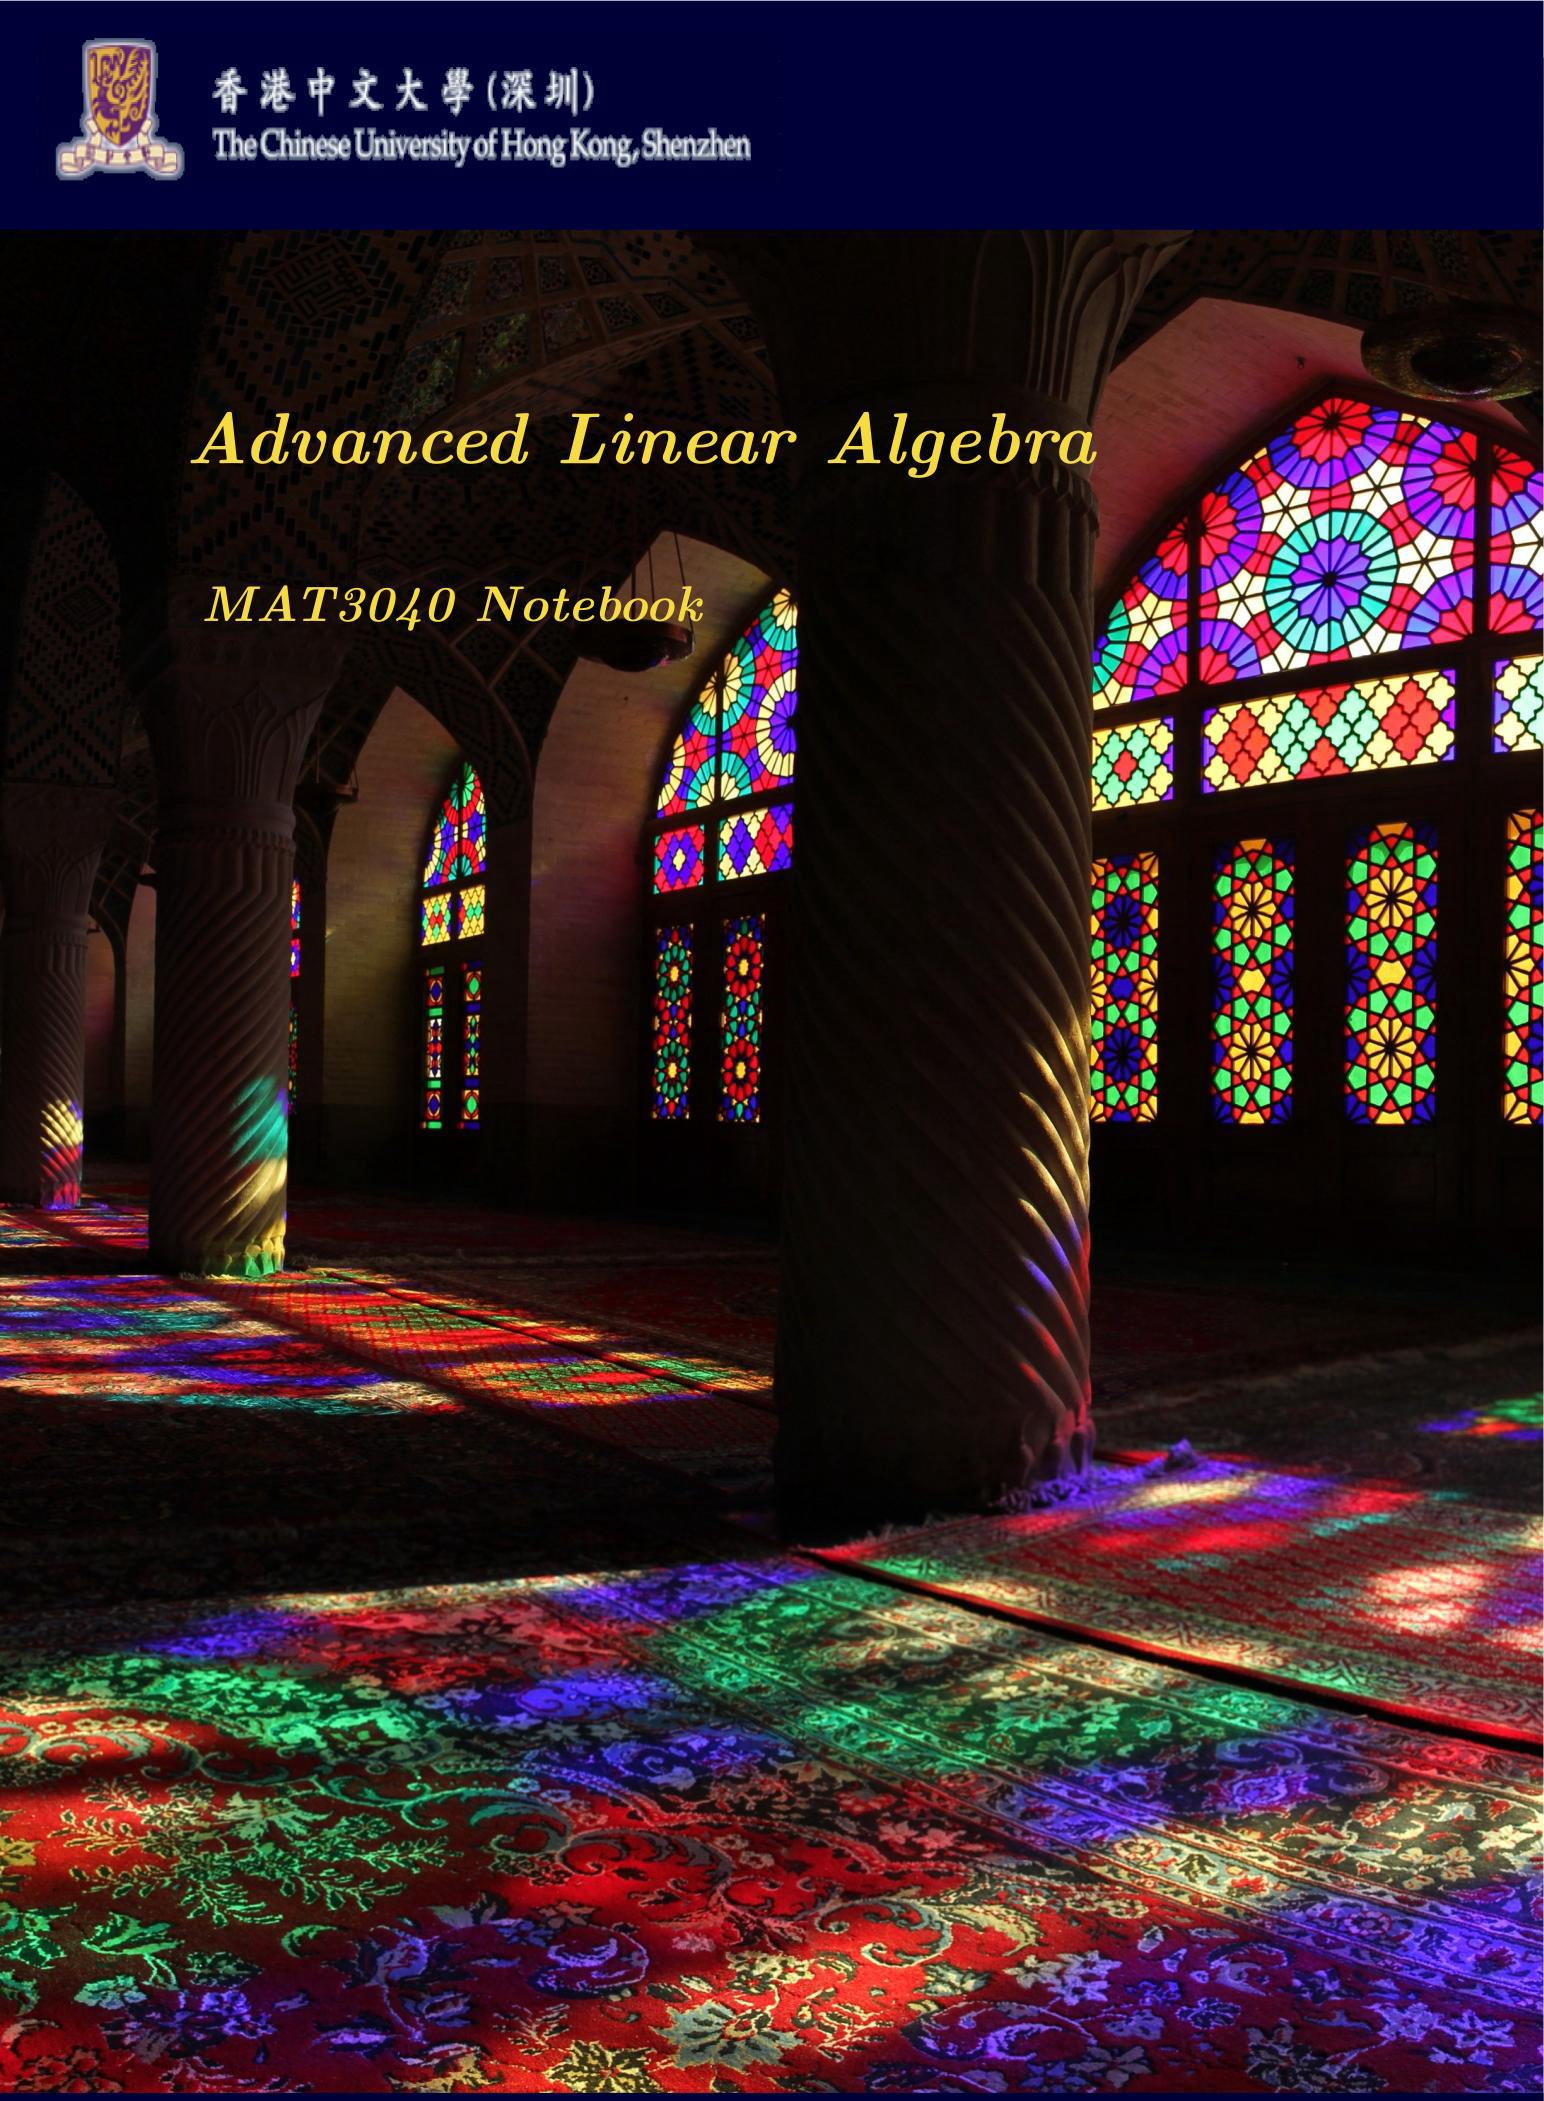
\includegraphics{images/bo_d1h964v7aajc7382l5mg_0_0_0_1544_2101_0.jpg}}
\end{center}


\author{Prof. Daniel Wong and Prof. Jie Wang}

\newpage
\tableofcontents

\newpage
\section*{Foreword}

This book is taken notes from the MAT 3040 in spring semester, 2019. These lecture notes were taken and compiled in \LaTeX\ by Jie Wang, an undergraduate student in spring 2019. The tex writter would like to thank Prof. Daniel Wong and some students for their detailed and valuable comments and suggestions, which significantly improved the quality of this notebook. Students taking this course may use the notes as part of their reading and reference materials. This version of the lecture notes were revised and extended for many times, but may still contain many mistakes and typos, including English grammatical and spelling errors, in the notes. It would be greatly appreciated if those students, who will use the notes as their reading or reference material, tell any mistakes and typos to Jie Wang for improving this notebook.

\newpage
\section*{Notations and Conventions}

\begin{tabular}{rl}
\({\mathbb{F}}^n\) & \(n\)-dimensional \(\mathbb{F}\)-valued space\\

 \({M}_{m \times  n}\left( \mathbb{F}\right)\) &set of all \((m \times  n)\) \(\mathbb{F}\)-valued matrices\\

 \(\oplus  \) & Direct Sum \\

 \(\ker \left( T\right) \) & The null space of \(T\)\\

 \(V \cong  W\) & vector spaces \(V\) and \(W\) are isomorphic\\

 \({\left( T\right) }_{\mathcal{B},\mathcal{A}}\) & Matrix representation of \(T\) w.r.t. \(\mathcal{A}\) and \(\mathcal{B}\)\\

 \(\mathbf{v} + W\) & coset of \(\mathbf{v}\) in $W \leq V$, i.e., \(\{ \mathbf{v} + \mathbf{w} \mid  \mathbf{w} \in  W\}\)\\

 \({A}_{i}^{\mathrm{T}}\)& \(i^{th}\) row of matrix \(A\)\\

  \(V/W\) & Quotient space of \(V\) by the subspace \(W \leq V\)\\

  \(V^*\)& Dual space of \(V\), i.e. the set of linear transformations from \(V\) to \(\mathbb{F}\)\\

  \(\mathrm{Ann}\left( S\right) \) & The annihilator of \(S \subseteq  V\), i.e. \(\left\{  {f \in  {V}^{ * } \mid  f\left( s\right)  = 0,\forall s \in  S}\right\}\)\\

 \({T}^{ * } : {W}^{ * } \rightarrow  {V}^{ * }\) & Adjoint map  for the mapping \(T : V \rightarrow  W\)\\

\(A^t\) & transpose of \(A\), i.e, \(B = A^t\) means \({b}_{ji} = {{a}}_{ij}\) for all \(i,j\)\\

 \(A^{\mathrm{H}}\) & Hermitian transpose of \(A\), i.e, \(B = A^{\mathrm{H}}\) means \({b}_{ji} = {\bar{a}}_{ij}\) for all \(i,j\)\\

 \({\mathcal{X}}_{T}\left( x\right) \) & characteristic polynomial of \(T\)\\

 \({m}_{T}\left( x\right) \) & Minimal polynomial of the linear operator \(T\)\\

 \({T}^{\prime } : V \rightarrow  V\) & Hermitian Adjoint for \(T : V \rightarrow  V\)\\

 \(\langle \mathbf{v},\mathbf{w}\rangle \) & Inner product between vectors \(\mathbf{v}\) and \(\mathbf{w}\)\\

 \(V \otimes  W\) & Tensor product between vector spaces \(V\) and \(W\)\\

 \(V \land  V\) & Wedge product for vector space \(V\)
\end{tabular}


\newpage

\section{Week 1}

\subsection{Introduction}

Advanced Linear Algebra (MAT 3040) is one of the most important courses in MATH major, with prerequisite MAT 2040 and MAT 1001/1011. This course will offer {\bf true} linear algebra knowledge. 

\medskip

{\bf What will be covered?}
\begin{itemize}
\item In MAT 2040 we have studied the space \({\mathbb{R}}^n\) ; while in MAT 3040 we will study the general vector space \(V\).

\item In MAT 2040 we have studied the linear transformation between Euclidean spaces, i.e., \(T : {\mathbb{R}}^n \rightarrow  {\mathbb{R}}^{m}\) ; while in MAT 3040 we will study the linear transformation from vector spaces to vector spaces: \(T : V \rightarrow  W\)

\item In MAT 2040 we have studied the eigenvalues of \(n \times  n\) matrix \(A\) ; while in MAT 3040 we will study the eigenvalues of a linear operator \(T : V \rightarrow  V\).

\item In MAT 2040 we have studied the dot product \(\mathbf{x} \cdot  \mathbf{y} = \mathop{\sum }\limits_{{i = 1}}^n{x}_{i}{y}_{i}\) ; while in MAT 3040 we will study the inner product \(\left\langle  {{\bf v}_1,{\bf v}_2}\right\rangle\).
\end{itemize}

{\bf Why generalize?} In mathematics (and beyond), we come across many other spaces than $\mathbb{R}^n$, for example:
\begin{itemize}
\item \(\mathcal{C}\left( \mathbb{R}\right)\), the space of all functions on \(\mathbb{R}\),
\item \({\mathcal{C}}^{\infty }\left( \mathbb{R}\right)\), the space of all infinitely differentiable functions on \(\mathbb{R}\),
\item \(\mathbb{R}[x]\), the space of polynomials of one real variable.
\end{itemize}

Here are some applications in partial differential equations and physics:
\begin{example}
1. Consider the Laplace equation \({\Delta f} = 0\) with Laplace operator:

\[
\Delta  : {C}^{\infty }\left( {\mathbb{R}}^{3}\right)  \rightarrow  {C}^{\infty }\left( {\mathbb{R}}^{3}\right), \quad \quad f \mapsto  \left( {\frac{{\partial }^2}{\partial {x}^2} + \frac{{\partial }^2}{\partial {y}^2} + \frac{{\partial }^2}{\partial {z}^2}}\right) f
\]
The solution to the partial differential equation \({\Delta f} = 0\) is the $0$-eigenspace of \(\Delta\).

\medskip
2. Consider the Schrödinger equation \(\widehat{H}f = {Ef}\) with the Schrödinger operator
\[
\widehat{H} : {C}^{\infty }\left( {\mathbb{R}}^{3}\right)  \rightarrow  {C}^{\infty }\left( {\mathbb{R}}^{3}\right),\quad \quad f \mapsto  \left(  {\frac{-{\hslash }^2}{2\mu }{\nabla }^2 + V\left( {x,y,z}\right) }\right)  f
\]

Solving the equation \(\widehat{H}f = \lambda f\) is equivalent to finding the $\lambda$-eigenspace of \(\widehat{H}\). In fact, a major observation in quantum mechanics is that the eigenvalues of \(\widehat{H}\) are discrete.    
\end{example}


\subsection{Vector Spaces}

\begin{definition}[Vector Space] A {\bf vector space} over a field \(\mathbb{F}\) (in particular, \(\mathbb{F} = \mathbb{R}\) or \(\mathbb{C}\)) is a set of objects \(V\) equipped with vector addiction $+$ and scalar multiplication $\cdot$ such that the following rules are satisfied:
\begin{itemize}
    \item Commutativity: \({\bf v}_1 + {\bf v}_2 = {\bf v}_2 + {\bf v}_1\).

    \item Associativity: \({\bf v}_1 + \left( {{\bf v}_2 + {\bf v}_{3}}\right)  = \left( {{\bf v}_1 + {\bf v}_2}\right)  + {\bf v}_{3}\).

    \item Zero vector: there exists \(\mathbf{0} \in  V\) such that \(\mathbf{0} + \mathbf{v} = \mathbf{v}\) for all \(\mathbf{v} \in  V\).

    \item Additive inverse: for all ${\bf v} \in V$, there exists \(-{\bf v} \in V\) such that ${\bf v} + (-{\bf v}) = {\bf 0}$.

    \item Distributivity of vectors: \(\alpha \left( {{\bf v}_1 + {\bf v}_2}\right)  = \alpha {\bf v}_1 + \alpha {\bf v}_2\).

    \item Distributivity of scalars: \(\left( {\alpha_1 + \alpha_2}\right) \mathbf{v} = \alpha_1\mathbf{v} + \alpha_2\mathbf{v}\).

    \item Compatibility of scalar multiplication: \(\alpha_1\left( {\alpha_2\mathbf{v}}\right)  = \left( {\alpha_1\alpha_2}\right) \mathbf{v}\).

    \item Multiplicative identity: \(1\mathbf{v} = \mathbf{v}\).
\end{itemize}
\end{definition}

Here we study several examples of vector spaces:

\begin{example} For \(V = {\mathbb{F}}^n\), we can define scalar multiplication:
\[
\alpha \left( \begin{matrix} {x}_1 \\  \vdots \\  {x}_n \end{matrix}\right)  = \left( \begin{matrix} \alpha {x}_1 \\  \vdots \\  \alpha {x}_n \end{matrix}\right)
\]
and vector addition:
\[
\left( \begin{matrix} {x}_1 \\  \vdots \\  {x}_n \end{matrix}\right)  + \left( \begin{matrix} {y}_1 \\  \vdots \\  {y}_n \end{matrix}\right)  = \left( \begin{matrix} {x}_1 + {y}_1 \\  \vdots \\  {x}_n + {y}_n \end{matrix}\right).
\]
In such a case,
\(
\mathbf{0} = \left( \begin{matrix} 0 \\  \vdots \\  0 \end{matrix}\right)
\) is the zero vector.
\end{example}

\begin{example}
It is clear that the set \(V = {M}_{m \times  n}\left( \mathbb{F}\right)\) (the set of all \(m \times  n\) real matrices) is a vector space as well. In such a case, the zero `vector' is the zero matrix ${\bf 0}_{m \times n}$.
\end{example}

\begin{example}
The set \(V = \mathcal{C}\left( \mathbb{R}\right)\) is a vector space with scalar multiplication:
\[
\left( {\alpha f}\right) \left( x\right)  = {\alpha f}\left( x\right) ,\forall \alpha  \in  \mathbb{R},f \in  V
\]    
and vector addition:
\[
\left( {f + g}\right) \left( x\right)  = f\left( x\right)  + g\left( x\right) ,\forall f,g \in  V
\]
Here the zero vector is the zero function, i.e., \(\mathbf{0}\left( x\right)  = 0\) for all \(x \in  \mathbb{R}\).
\end{example}


\begin{definition} A sub-collection \(W \subseteq  V\) of a vector space \(V\) is called a {\bf vector subspace} of \(V\) if \(W\) itself forms a vector space, denoted by \(W \leq  V\).
\end{definition}

\begin{example} 
For \(V = {\mathbb{R}}^{3}\), \(W := \{ \left( {x,y,0}\right)  \mid  x,y \in  \mathbb{R}\}  \leq  V\), but \(W' := \{ \left( {x,y,1}\right)  \mid  x,y \in  \mathbb{R}\}\) is not a vector subspace of \(V\).
\end{example}

\begin{proposition} A subset \(W \subseteq  V\) is a vector subspace of \(V\) iff for all \({\bf w}_1,{\bf w}_2 \in  W\), we have 
\[\alpha \mathbf{\bf w}_1 + \beta {\bf w}_2 \in  W\] 
for all \(\alpha ,\beta  \in  \mathbb{F}\).
\end{proposition}
The proof is identical to that of MAT 2040.


\begin{example} 
We look at a few more examples and non-examples of vector subspaces:
\begin{itemize}
    \item Let \(V = {M}_{n \times  n}\left( \mathbb{F}\right)\), then the subset of all symmetric matrices \(W = \left\{  A \in  V \mid  {A^t = A}\right\}   \leq  V\) is a subspace of $V$.

    \item Let \(V = {C}^{\infty }\left( \mathbb{R}\right)\). Define \(W = \left\{  {f \in  V \mid  \frac{{\mathrm{d}}^2}{\mathrm{\;d}{x}^2}f + f = 0}\right\}   \leq  V\). For \(f,g \in  W\), we have
\[
{\left( \alpha f + \beta g\right) }^{\prime \prime } = \alpha {f}^{\prime \prime } + \beta {g}^{\prime \prime } = \alpha \left( {-f}\right)  + \beta \left( {-g}\right)  =  - \left( {{\alpha f} + {\beta g}}\right) ,
\]

which implies \({\left( \alpha f + \beta g\right) }^{\prime \prime } + \left( {{\alpha f} + {\beta g}}\right)  = 0\). Therefore, $W \leq V$.

\item Let \(V = {\mathbb{R}}^2\). Then the set \( {\mathbb{R}}_{ + }^2 := \{(x,y) \in \mathbb{R}^2\ | x, y > 0\}\) is not a vector subspace, since \(W\) is not closed under scalar multiplication.

\item Moreover, the set \({\mathbb{R}}_{ + }^2 \cup {\mathbb{R}}_{ - }^2 := \{(x,y) \in \mathbb{R}^2\ | xy > 0\} \) is not a vector subspace of $V = \mathbb{R}^2$ since it is not closed under addition.

\item For \(V = {\mathbb{M}}_{3 \times  3}\left( \mathbb{R}\right)\), the set of invertible \(3 \times  3\) matrices is not a vector subspace, since the zero `vector' ${\bf0}_{3 \times 3}$ is not invertible (Exercise: How about the set of all singular matrices?).
\end{itemize}
\end{example}

\subsection{Spanning Set}

\begin{definition} Let \(V\) be a vector space over \(\mathbb{F}\) :

1. A {\bf linear combination} of a subset \(S\) in \(V\) is of the form
\[
\mathop{\sum }\limits_{{i = 1}}^n\alpha_{i}{\mathbf{s}}_{i},\quad \alpha_{i} \in  \mathbb{F},{\mathbf{s}}_{i} \in  S
\]
for $n \in \mathbb{N}$. Note that the summation should be finite.

2. The {\bf span} of a subset \(S \subseteq  V\) is
\[
\operatorname{span}\left( S\right)  = \left\{  {\mathop{\sum }\limits_{{i = 1}}^n\alpha_{i}{\mathbf{s}}_{i} \Big|  \alpha_{i} \in  \mathbb{F},{\mathbf{s}}_{i} \in  S}\right\}
\]

3. \(S\) is a {\bf spanning set} of \(V\), or say \(S\) {\bf spans} \(V\), if
\[
\operatorname{span}\left( S\right)  = V\text{ . }
\]
\end{definition}

\begin{example} 

\begin{enumerate}
    \item For \(V = \mathbb{R}\left\lbrack  x\right\rbrack\), define the set \(S := \left\{  {1,{x}^2,{x}^{4},\ldots ,{x}^{6}}\right\} \subseteq V\). Then \(2 + {x}^{4} + \pi {x}^{106} \in  \operatorname{span}\left( S\right)\), while the series \(1 + {x}^2 + {x}^{4} + \cdots  \notin  \operatorname{span}\left( S\right)\). 

It is clear that \(\operatorname{span}\left( S\right)  \neq  V\), but \(S\) is the spanning set of \(W = \{ p \in  V \mid  p\left( x\right)  = p\left( {-x}\right) \}\).

\item For \(V = {M}_{3 \times  3}\left( \mathbb{R}\right)\), let \({\bf w}_1 = \left\{  {A \in  V \mid  {A}^{\mathrm{T}} = A}\right\}\) and \({\bf w}_2 = \left\{  {B \in  V \mid  {B}^{\mathrm{T}} =  - B}\right\}\) (the set of skew-symmetric matrices) be two vector subspaces. {\bf Exercise:} show that the set \( S := {\bf w}_1\cup {\bf w}_2\) spans \(V\).
\end{enumerate}
\end{example}


\begin{proposition} \label{prop:exchangelem}
Let \(S\) be a subset in a vector space \(V\).

\begin{enumerate}
\item \(S \subseteq  \operatorname{span}\left( S\right)\)

\item \(\operatorname{span}\left( S\right)  = \operatorname{span}\left( {\operatorname{span}\left( S\right) }\right)\)

\item (Exchange Lemma) If \(\mathbf{w} \in  \operatorname{span}\left\{  {{\bf v}_1,\ldots ,{\bf v}_n}\right\}   \smallsetminus  \operatorname{span}\left\{  {{\bf v}_2,\ldots ,{\bf v}_n}\right\}\), then

\[
{\bf v}_1 \in  \operatorname{span}\left\{  {\mathbf{w},{\bf v}_2,\ldots ,{\bf v}_n}\right\}   \smallsetminus  \operatorname{span}\left\{  {{\bf v}_2,\ldots ,{\bf v}_n}\right\}
\]
\end{enumerate}
\end{proposition}

\begin{proof} 
1. For each \(s \in  S\), we have

\[
\mathbf{s} = 1 \cdot  \mathbf{s} \in  \operatorname{span}\left( S\right)
\]

2. From (1), it’s clear that \(\operatorname{span}\left( S\right)  \subseteq  \operatorname{span}\left( {\operatorname{span}\left( S\right) }\right)\), and therefore suffices to show

\(\operatorname{span}\left( {\operatorname{span}\left( S\right) }\right)  \subseteq  \operatorname{span}\left( S\right)\) :

Pick \(\mathbf{v} = \mathop{\sum }\limits_{{i = 1}}^n\alpha_{i}{\bf v}_{i} \in  \operatorname{span}\left( {\operatorname{span}\left( S\right) }\right)\), where \({\bf v}_{i} \in  \operatorname{span}\left( S\right)\). Rewrite

\[
{\bf v}_{i} = \mathop{\sum }\limits_{{j = 1}}^{n_{i}}\beta_{ij}{\mathbf{s}}_{j},\;{\mathbf{s}}_{j} \in  S,
\]

which implies

\[
\mathbf{v} = \mathop{\sum }\limits_{{i = 1}}^n\alpha_{i}\mathop{\sum }\limits_{{j = 1}}^{n_{i}}\beta_{ij}{\mathbf{s}}_{j} = \mathop{\sum }\limits_{{i = 1}}^n\mathop{\sum }\limits_{{j = 1}}^{n_{i}}\left( {\alpha_{i}\beta_{ij}}\right) {\mathbf{s}}_{j},
\]

i.e., \(\bf v\) is a finite linear combination of elements in \(S\), which implies \({\bf v} \in  \operatorname{span}\left( S\right)\).

3. By hypothesis, \(\mathbf{w} = \alpha_1{\bf v}_1 + \cdots  + \alpha_n{\bf v}_n\) with \(\alpha_1 \neq  0\), which implies
\[
{\bf v}_1 =  - \frac{\alpha_2}{\alpha_1}{\bf v}_2 + \cdots  + \left( {-\frac1{\alpha_1}\mathbf{w}}\right)
\]
which implies \({\bf v}_1 \in  \operatorname{span}\left\{  {\mathbf{w},{\bf v}_2,\ldots ,{\bf v}_n}\right\}\). It suffices to show \({\bf v}_1 \notin  \operatorname{span}\left\{  {{\bf v}_2,\ldots ,{\bf v}_n}\right\}\). Suppose on the contrary that \({\bf v}_1 \in  \operatorname{span}\left\{  {{\bf v}_2,\ldots ,{\bf v}_n}\right\}\). It’s clear that \(\operatorname{span}\left\{  {{\bf v}_1,\ldots ,{\bf v}_n}\right\}   =\)  \(\operatorname{span}\left\{  {{\bf v}_2,\ldots ,{\bf v}_n}\right\}\). (left as exercise). Therefore,
\[
\varnothing  = \operatorname{span}\left\{  {{\bf v}_1,\ldots ,{\bf v}_n}\right\}   \smallsetminus  \operatorname{span}\left\{  {{\bf v}_2,\ldots ,{\bf v}_n}\right\}  ,
\]

which is a contradiction.
\end{proof}


\subsection{Linear Independence and Basis}

\begin{definition}[Linear Independence] Let \(S\) be a (not necessarily finite) subset of \(V\). Then \(S\) is {\bf linearly independent} (l.i.) on \(V\) if for any finite subset \(\left\{  {{\mathbf{s}}_1,\ldots ,{\mathbf{s}}_{k}}\right\}\) in \(S\),

\[
\mathop{\sum }\limits_{{i = 1}}^{k}\alpha_{i}{\mathbf{s}}_{i} = 0 \Leftrightarrow  \alpha_{i} = 0\ \forall i.
\]
Otherwise, we say $S$ is {\bf linearly dependent}.
\end{definition}

\begin{example}
\begin{itemize}
\item For \(V = C\left( \mathbb{R}\right)\), \({S}_1 = \{ \sin x,\cos x\}\) is linearly independent, since
\[
\alpha \sin x + \beta \cos x = \mathbf{0}\text{ (means zero function) }
\]
Taking \(x = 0\) both sides leads to \(\beta  = 0\) ; taking \(x = \frac{\pi }2\) both sides leads to \(\alpha  = 0\).

\item For \(V = C\left( \mathbb{R}\right)\), \({S}_2 = \left\{  {{\sin }^2x,{\cos }^2x,1}\right\}\) is linearly dependent, since
\[
1 \cdot  {\sin }^2x + 1 \cdot  {\cos }^2x + \left( {-1}\right)  \cdot  1 = 0,\forall x
\]

\item For \(V = \mathbb{R}\left\lbrack  x\right\rbrack\), \(S = \left\{  {1,x,{x}^2,{x}^{3},\ldots ,}\right\}\) is linearly independent: Pick \({x}^{{k}_1},\ldots ,{x}^{{k}_n} \in  S\) with \({k}_1 < \cdots  < {k}_n\). Consider that the equation

\[
\alpha_1{x}^{{k}_1} + \cdots  + \alpha_n{x}^{{k}_n} = \mathbf{0}
\]

holds for all \(x\), and try to solve for \(\alpha_1,\ldots ,\alpha_n\) (one way is differentation.)
\end{itemize}
\end{example}


\begin{definition}[Basis] A subset \(S\) is a {\bf basis} of \(V\) if

(a) \(S\) spans \(V\); and

(b) \(S\) is linearly independent.
\end{definition}

\begin{example} 
1. For \(V = {\mathbb{R}}^n,S = \left\{  {{\mathbf{e}}_1,\ldots ,{\mathbf{e}}_n}\right\}\) is a basis of \(V\)

2. For \(V = \mathbb{R}\left\lbrack  x\right\rbrack  ,S = \left\{  {1,x,{x}^2,\ldots }\right\}\) is a basis of \(V\)

3. For \(V = {M}_{2 \times  2}\left( \mathbb{R}\right)\),
\[
S = \left\{  {\left( \begin{array}{ll} 1 & 0 \\  0 & 0 \end{array}\right) ,\left( \begin{array}{ll} 0 & 1 \\  0 & 0 \end{array}\right) ,\left( \begin{array}{ll} 0 & 0 \\  1 & 0 \end{array}\right) ,\left( \begin{array}{ll} 0 & 0 \\  0 & 1 \end{array}\right) }\right\}
\]
is a basis of \(V\).
\end{example}

\begin{proposition} Let \(V = \operatorname{span}\left\{  {{\bf v}_1,\ldots ,{\bf v}_{m}}\right\}\). Then there exists a subset of \(\left\{  {{\bf v}_1,\ldots ,{\bf v}_{m}}\right\}\) which is a basis of \(V\).
\end{proposition}

\begin{proof} If \(\left\{  {{\bf v}_1,\ldots ,{\bf v}_{m}}\right\}\) is linearly independent, the proof is complete. Otherwise, \(\alpha_1{\bf v}_1 + \cdots  + \alpha_{m}{\bf v}_{m} = \mathbf{0}\) has a non-trivial solution. w.l.o.g., \(\alpha_1 \neq  0\), which implies

\[
{\bf v}_1 =  - \frac{\alpha_2}{\alpha_1}{\bf v}_2 + \cdots  + \left( \frac{\alpha_{m}}{\alpha_1}\right) {\bf v}_{m} \Rightarrow  {\bf v}_1 \in  \operatorname{span}\left\{  {{\bf v}_2,\ldots ,{\bf v}_{m}}\right\}
\]

By the proof in Proposition \ref{prop:exchangelem} (3),
\[
V =\operatorname{span}\left\{  {{\bf v}_1,\ldots ,{\bf v}_{m}}\right\}   = \operatorname{span}\left\{  {{\bf v}_2,\ldots ,{\bf v}_{m}}\right\}  ,
\]
which implies \(V = \operatorname{span}\left\{  {{\bf v}_2,\ldots ,{\bf v}_{m}}\right\}\).
So one can continue this argument finitely many times until one has \(\left\{  {{\bf v}_{i},{\bf v}_{i + 1},\ldots ,{\bf v}_{m}}\right\}\) is linearly independent, and spans \(V\). The proof is complete.
\end{proof}


\begin{corollary}
Suppose \(V\) is {\bf finite-generated}, i.e. there exists a finite set $\{{\bf v}_1,\ldots ,{\bf v}_{m}\}$ such that $V = \operatorname{span}\left\{{\bf v}_1,\ldots ,{\bf v}_{m}\right\}$.
Then \(V\) has a basis. 
\end{corollary}
The same conclusion holds for non-finitely generated \(V\) if one assumes Zorn's lemma.


\begin{proposition} If \(\left\{  {{\bf v}_1,\ldots ,{\bf v}_n}\right\}\) is a basis of \(V\), then every \(v \in  V\) can be expressed uniquely as

\[
\mathbf{v} = \alpha_1{\bf v}_1 + \cdots  + \alpha_n{\bf v}_n
\]
\end{proposition}

\begin{proof} Since \(\left\{  {{\bf v}_1,\ldots ,{\bf v}_n}\right\}\) spans \(V\), so \(\mathbf{v} \in  V\) can be written as
\[
\mathbf{v} = \alpha_1{\bf v}_1 + \cdots  + \alpha_n{\bf v}_n
\]

Suppose further that
\[
\mathbf{v} = \beta_1{\bf v}_1 + \cdots  + \beta_n{\bf v}_n,
\]
for some $\beta_i \in \mathbb{F}$, it suffices to show that \(\alpha_{i} = \beta_{i}\) for all \(i\): Indeed, by subtracting the above equations, one has
\[
\left( {\alpha_1 - \beta_1}\right) {\bf v}_1 + \cdots  + \left( {\alpha_n - \beta_n}\right) {\bf v}_n = 0.
\]
By the hypothesis of linear independence, we have \(\alpha_{i} - \beta_{i} = 0\) for all \(i\), i.e., \(\alpha_{i} = \beta_{i}\).
\end{proof}

\newpage
\section{Week 2}
\subsection{Basis and Dimension}
We begin by showing that the bases of any finitely generated vector spaces have the same number of vectors:
\begin{theorem} Let \(V\) be a finitely generated vector space. Suppose \(\left\{  {{\bf v}_1,\ldots ,{\bf v}_{m}}\right\}\) and \(\left\{  {{\bf w}_1,\ldots ,{\bf w}_n}\right\}\) are two basis of \(V\). Then \(m = n\). 
\end{theorem}

\begin{proof} Suppose on the contrary that \(m \neq  n\). Without loss of generality, assume that \(m < n\). Let \({\bf v}_1 = \alpha_1{\bf w}_1 + \cdots  + \alpha_n{\bf w}_n\), with some \(\alpha_{i} \neq  0\). By rearranging the terms if necessary, assume \(\alpha_1 \neq  0\). Therefore,
\[
{\bf v}_1 \in  \operatorname{span}\left\{  {{\bf w}_1,{\bf w}_2,\ldots ,{\bf w}_n}\right\}   \smallsetminus  \operatorname{span}\left\{  {{\bf w}_2,\ldots ,{\bf w}_n}\right\}   \tag{2.1}
\]

which implies that \({\bf w}_1 \in  \operatorname{span}\left\{  {{\bf v}_1,{\bf w}_2,\ldots ,{\bf w}_n}\right\}   \smallsetminus  \operatorname{span}\left\{  {{\bf w}_2,\ldots ,{\bf w}_n}\right\}\).

Then we claim that \(\left\{  {{\bf v}_1,{\bf w}_2,\ldots ,{\bf w}_n}\right\}\) is a basis of \(V\) :

1. Note that \(\left\{  {{\bf v}_1,{\bf w}_2,\ldots ,{\bf w}_n}\right\}\) is a spanning set:

\begin{align*}
{\bf w}_1 \in  \operatorname{span}\left\{  {{\bf v}_1,{\bf w}_2,\ldots ,{\bf w}_n}\right\}  &\Rightarrow  \left\{  {{\bf w}_1,{\bf w}_2,\ldots ,{\bf w}_n}\right\}   \subseteq  \operatorname{span}\left\{  {{\bf v}_1,{\bf w}_2,\ldots ,{\bf w}_n}\right\}
\\
&\Rightarrow  \operatorname{span}\left\{  {{\bf w}_1,{\bf w}_2,\ldots ,{\bf w}_n}\right\}   \subseteq  \operatorname{span}\left\{  {\operatorname{span}\left\{  {{\bf v}_1,{\bf w}_2,\ldots ,{\bf w}_n}\right\}  }\right\}   =\operatorname{span}\left\{  {{\bf v}_1,{\bf w}_2,\ldots ,{\bf w}_n}\right\}
\end{align*}

Since \(V = \operatorname{span}\left\{  {{\bf w}_1,{\bf w}_2,\ldots ,{\bf w}_n}\right\}\), we have \(\operatorname{span}\left\{  {{\bf v}_1,{\bf w}_2,\ldots ,{\bf w}_n}\right\}   = V\).

2. Then we show the linear independence of \(\left\{  {{\bf v}_1,{\bf w}_2,\ldots ,{\bf w}_n}\right\}\). Consider the equation

\[
\beta_1{\bf v}_1 + \beta_2{\bf v}_2 + \cdots  + \beta_n{\bf w}_n = \mathbf{0}
\]

(a) When \(\beta_1 \neq  0\), we imply

\[
{\bf v}_1 = \left( {-\frac{\beta_2}{\beta_1}}\right) {\bf w}_2 + \cdots  + \left( {-\frac{\beta_n}{\beta_1}}\right) {\bf w}_n \in  \operatorname{span}\left\{  {{\bf w}_2,\ldots ,{\bf w}_n}\right\}  ,
\]

which contradicts (2.1).

(b) When \(\beta_1 = 0\), then \(\beta_2{\bf w}_2 + \cdots  + \beta_n{\bf w}_n = \mathbf{0}\), which implies \(\beta_2 = \cdots  = \beta_n = 0\), due

to the independence of \(\left\{  {{\bf w}_2,\ldots ,{\bf w}_n}\right\}\).

Therefore, \({\bf v}_2 \in  \operatorname{span}\left\{  {{\bf v}_1,{\bf w}_2,\ldots ,{\bf w}_n}\right\}\), i.e.,

\[
{\bf v}_2 = {\gamma }_1{\bf v}_1 + \cdots  + {\gamma }_n{\bf v}_n
\]

where \({\gamma }_2,\ldots ,{\gamma }_n\) cannot be all zeros, since otherwise \(\left\{  {{\bf v}_1,{\bf v}_2}\right\}\) are linearly dependent, i.e., \(\left\{  {{\bf v}_1,\ldots ,{\bf v}_{m}}\right\}\) cannot form a basis. w.l.o.g., assume \({\gamma }_2 \neq  0\), which implies

\[
{\bf w}_2 \in  \operatorname{span}\left\{  {{\bf v}_1,{\bf v}_2,{\bf w}_{3},\ldots ,{\bf w}_n}\right\}   \smallsetminus  \operatorname{span}\left\{  {{\bf v}_1,{\bf w}_{3},\ldots ,{\bf w}_n}\right\}  .
\]

Following the similar argument above, \(\left\{  {{\bf v}_1,{\bf v}_2,{\bf w}_{3},\ldots ,{\bf w}_n}\right\}\) forms a basis of \(V\).

Continuing the argument above, we imply \(\left\{  {{\bf v}_1,\ldots ,{\bf v}_{m},{\bf w}_{m + 1},\ldots ,{\bf w}_n}\right\}\) is a basis of \(V\).

Since \(\left\{  {{\bf v}_1,\ldots ,{\bf v}_{m}}\right\}\) is a basis as well, we imply

\[
{\bf w}_{m + 1} = {\delta }_1{\bf v}_1 + \cdots  + {\delta }_{m}{\bf v}_{m}
\]

for some \({\delta }_{i} \in  \mathbb{F}\), i.e., \(\left\{  {{\bf v}_1,\ldots ,{\bf v}_{m},{\bf w}_{m + 1}}\right\}\) is linearly dependent, which is a contradiction.
\end{proof}


\begin{itemize}
\item Example 2.1 A vector space may have more than one basis.
\end{itemize}

Suppose \(V = {\mathbb{F}}^n\), it is clear that \(\dim \left( V\right)  = n\), and

\(\left\{  {{\mathbf{e}}_1,\ldots ,{\mathbf{e}}_n}\right\}\) is a basis of \(V\), where \({\mathbf{e}}_{i}\) denotes a unit vector.

There could be other basis of \(V\), such as

\[
\left\{  {\left( \begin{matrix} 1 \\  0 \\  0 \\  \vdots \\  0 \end{matrix}\right) ,\left( \begin{matrix} 1 \\  1 \\  0\\  \vdots \\  0 \end{matrix}\right) ,\cdots ,\left( \begin{matrix} 1 \\  1 \\  1\\  \vdots \\  1 \end{matrix}\right) }\right\}
\]

Actually, the columns of any invertible \(n \times  n\) matrix forms a basis of \(V\).

\begin{itemize}
\item Example 2.2 Suppose \(V = {M}_{m \times  n}\left( \mathbb{R}\right)\), we claim that \(\dim \left( V\right)  = {mn}\) :
\end{itemize}

\[
\left\{  {{E}_{ij}\left| {\;\begin{array}{l} 1 \leq  i \leq  m \\  1 \leq  j \leq  n \end{array}}\right. }\right\}  \text{ is a basis of }V\text{ , }
\]

where \({E}_{ij}\) is \(m \times  n\) matrix with 1 at(i, j)-th entry, and 0 s at the remaining entries.

\begin{itemize}
\item Example 2.3 Suppose \(V = \{\) all polynomials of degree \(\leq  \mathrmn\}\), then \(\dim \left( V\right)  = n + 1\).
\end{itemize}

\begin{itemize}
\item Example 2.4 Supppose \(V = \left\{  {A \in  {M}_{n \times  n}\left( \mathbb{R}\right)  \mid  {A}^{\mathrm{T}} = A}\right\}\), then \(\dim \left( V\right)  = \frac{n\left( {n + 1}\right) }2\).
\end{itemize}

\begin{itemize}
\item Example 2.5 Let \(W = \left\{  {B \in  {M}_{n \times  n}\left( \mathbb{R}\right)  \mid  {B}^{\mathrm{T}} =  - B}\right\}\), then \(\dim \left( V\right)  = \frac{n\left( {n - 1}\right) }2\).
\end{itemize}

Sometimes it should be classified the field \(\mathbb{F}\) for the scalar multiplication to define a vector space. Conside the example below:

1. Let \(V = \mathbb{C}\), then \(\dim \left( \mathbb{C}\right)  = 1\) for the scalar multiplication defined under the field \(\mathbb{C}\).

2. Let \(V = \operatorname{span}\{ 1,i\}  = \mathbb{C}\), then \(\dim \left( \mathbb{C}\right)  = 2\) for the scalar multiplication defined under the field \(\mathbb{R}\), since all \(z \in  V\) can be written as \(z = a + {bi}\), \(\forall a,b \in  \mathbb{R}\).

3. Therefore, to aviod confusion, it is safe to write

\[
{\dim }_{\mathbb{C}}\left( \mathbb{C}\right)  = 1,\;{\dim }_{\mathbb{R}}\left( \mathbb{C}\right)  = 2.
\]

\section*{2.1.2. Operations on a vector space}

Note that the basis for a vector space is characterized as the maximal linearly independent set.

Theorem 2.2 - Basis Extension. Let \(V\) be a finite dimensional vector space, and \(\left\{  {{\bf v}_1,\ldots ,{\bf v}_{k}}\right\}\) be a linearly independent set on \(V\), Then we can extend it to the basis \(\left\{  {{\bf v}_1,\ldots ,{\bf v}_{k},{\bf v}_{k + 1},\ldots ,{\bf v}_n}\right\}\) of \(V\).

Proof. - Suppose \(\dim \left( V\right)  = n > k\), and \(\left\{  {{\bf w}_1,\ldots ,{\bf w}_n}\right\}\) is a basis of \(V\). Consider the set \(\left\{  {{\bf w}_1,\ldots ,{\bf w}_n}\right\}   \cup  \left\{  {{\bf v}_1,\ldots ,{\bf v}_{k}}\right\}\), which is linearly dependent, i.e.,

\[
\alpha_1{\bf w}_1 + \cdots  + \alpha_n{\bf w}_n + \beta_1{\bf v}_1 + \cdots  + \beta_{k}{\bf v}_{k} = \mathbf{0},
\]

with some \(\alpha_{i} \neq  0\), since otherwise this equation will only have trivial solution. w.l.o.g., assume \(\alpha_1 \neq  0\).

\begin{itemize}
\item Therefore, consider the set \(\left\{  {{\bf w}_2,\ldots ,{\bf w}_n}\right\}   \cup  \left\{  {{\bf v}_1,\ldots ,{\bf v}_{k}}\right\}\). We keep removing elements from \(\left\{  {{\bf w}_2,\ldots ,{\bf w}_n}\right\}\) until we first get the set
\end{itemize}

\[
S\bigcup \left\{  {{\bf v}_1,\ldots ,{\bf v}_{k}}\right\}
\]

with \(S \subseteq  \left\{  {{\bf w}_1,{\bf w}_2,\ldots ,{\bf w}_n}\right\}\) and \(S \cup  \left\{  {{\bf v}_1,\ldots ,{\bf v}_{k}}\right\}\) is linearly independent, i.e., \(S\) is a maximal subset of \(\left\{  {{\bf w}_1,\ldots ,{\bf w}_n}\right\}\) such that \(S \cup  \left\{  {{\bf v}_1,\ldots ,{\bf v}_{k}}\right\}\) is linearly independent.

\begin{itemize}
\item Rewrite \(S = \left\{  {{\bf v}_{k + 1},\ldots ,{\bf v}_{m}}\right\}\) and therefore \({S}^{\prime } = \left\{  {{\bf v}_1,\ldots ,{\bf v}_{k},{\bf v}_{k + 1},\ldots ,{\bf v}_{m}}\right\}\) are linearly independent. It suffices to show \({S}^{\prime }\) spans \(V\).
\end{itemize}

\begin{itemize}
\item Indeed, for all \({\bf w}_{i} \in  \left\{  {{\bf w}_1,\ldots ,{\bf w}_n}\right\}  ,{\bf w}_{i} \in  \operatorname{span}\left( {S}^{\prime }\right)\), since otherwise the equation
\end{itemize}

\[
\alpha {\bf w}_{i} + \beta_1{\bf v}_1 + \cdots  + \beta_{m}{\bf v}_{m} = \mathbf{0} \Rightarrow  \alpha  = 0,
\]

which implies that \(\beta_1{\bf v}_1 + \cdots  + \beta_{m}{\bf v}_{m} = \mathbf{0}\) admits only trivial solution, i.e.,

\[
\left\{  {\bf w}_{i}\right\}  \bigcup {S}^{\prime } = \left\{  {\bf w}_{i}\right\}  \bigcup S\bigcup \left\{  {{\bf v}_1,\ldots ,{\bf v}_{k}}\right\}  \text{ is linearly independent, }
\]

which violetes the maximality of \(S\).

Therefore, all \(\left\{  {{\bf w}_1,\ldots ,{\bf w}_n}\right\}   \subseteq  \operatorname{span}\left( {S}^{\prime }\right)\), which implies \(\operatorname{span}\left( {S}^{\prime }\right)  = V\).

Therefore, \({S}^{\prime }\) is a basis of \(V\).

Start with a spanning set, we keep removing something to form a basis; start with independent set, we keep adding something to form a basis.

In other words, the basis is both the minimal spanning set, and the maximal linearly independent set.

Definition 2.1 [Direct Sum] Let \({\bf w}_1,{\bf w}_2\) be two vector subspaces of \(V\), then

1. \({\bf w}_1 \cap  {\bf w}_2 \mathrel{\text{ := }} \left\{  {\mathbf{w} \in  V \mid  \mathbf{w} \in  {\bf w}_1\text{ , and }\mathbf{w} \in  {\bf w}_2}\right\}\)

2. \({\bf w}_1 + {\bf w}_2 \mathrel{\text{ := }} \left\{  {{\bf w}_1 + {\bf w}_2 \mid  {\bf w}_{i} \in  {\bf w}_{i}}\right\}\)

3. If furthermore that \({\bf w}_1 \cap  {\bf w}_2 = \{ \mathbf{0}\}\), then \({\bf w}_1 + {\bf w}_2\) is denoted as \({\bf w}_1 \oplus  {\bf w}_2\), which is called direct sum.

Proposition \({2.1}\;{\bf w}_1 \cap  {\bf w}_2\) and \({\bf w}_1 + {\bf w}_2\) are vector subspaces of \(V\).

\section*{2.4. Wednesday for MAT 3040}

Reviewing.

\begin{itemize}
\item Basis, Dimension
\end{itemize}

\begin{itemize}
\item Basis Extension
\end{itemize}

\begin{itemize}
\item \({\bf w}_1 \cap  {\bf w}_2 = \varnothing\) implies \({\bf w}_1 \oplus  {\bf w}_2 = {\bf w}_1 + {\bf w}_2\) (Direct Sum).
\end{itemize}

\section*{2.4.1. Remark on Direct Sum}

Proposition 2.13 The set \({\bf w}_1 + {\bf w}_2 = {\bf w}_1 \oplus  {\bf w}_2\) iff any \(\mathbf{w} \in  {\bf w}_1 + {\bf w}_2\) can be uniquely expressed as

\[
w = {\bf w}_1 + {\bf w}_2
\]

where \({\bf w}_{i} \in  {\bf w}_{i}\) for \(i = 1,2\).

R) We can also define addiction among finite set of vector spaces \(\left\{  {{\bf w}_1,\ldots ,{\bf w}_{k}}\right\}\).

If \({\bf w}_1 + \cdots  + {\bf w}_{k} = \mathbf{0}\) implies \({\bf w}_{i} = 0,\forall i\), then we can write \({\bf w}_1 + \cdots  + {\bf w}_{k}\) as

\({\bf w}_1 \oplus  \cdots  \oplus  {\bf w}_{k}\)

Proposition 2.14 - Complementation. Let \(W \leq  V\) be a vector subspace of a fintie dimension vector space \(V\). Then there exists \({W}^{\prime } \leq  V\) such that

\[
W \oplus  {W}^{\prime } = V
\]

Proof. It’s clear that \(\dim \left( W\right)  \mathrel{\text{ := }} k \leq  n \mathrel{\text{ := }} \dim \left( V\right)\). Suppose \(\left\{  {{\bf v}_1,\ldots ,{\bf v}_{k}}\right\}\) is a basis of \(W\).

By the basis extension proposition, we can extend it into \(\left\{  {{\bf v}_1,\ldots ,{\bf v}_{k},{\bf v}_{k + 1},\ldots ,{\bf v}_n}\right\}\), which is a basis of \(V\).

Therefore, we take \({W}^{\prime } = \operatorname{span}\left\{  {{\bf v}_{k + 1},\ldots ,{\bf v}_n}\right\}\), which follows that

1. \(W + {W}^{\prime } = V : \forall \mathbf{v} \in  V\) has the form

\[
\mathbf{v} = \left( {\alpha_1{\bf v}_1 + \cdots  + \alpha_{k}{\bf v}_{k}}\right)  + \left( {\alpha_{k + 1}{\bf v}_{k + 1} + \cdots  + \alpha_n{\bf v}_n}\right) ,
\]

where \(\alpha_1{\bf v}_1 + \cdots  + \alpha_{k}{\bf v}_{k} \in  W\) and \(\alpha_{k + 1}{\bf v}_{k + 1} + \cdots  + \alpha_n{\bf v}_n \in  {W}^{\prime }\).

2. \(W \cap  {W}^{\prime } = \{ \mathbf{0}\}\) : Suppose \(v \in  W \cap  {W}^{\prime }\), i.e.,

\[
\mathbf{v} = \left( {\beta_1{\bf v}_1 + \cdots  + \beta_{k}{\bf v}_{k}}\right)  + \left( {0{\bf v}_{k + 1} + \cdots  + 0{\bf v}_n}\right)  \in  W
\]

\[
= \left( {0{\bf v}_1 + \cdots  + 0{\bf v}_{k}}\right)  + \left( {\beta_{k + 1}{\bf v}_{k + 1} + \cdots  + \beta_n{\bf v}_n}\right)  \in  {W}^{\prime }.
\]

By the uniqueness of coordinates, we imply \(\beta_1 = \cdots  = \beta_n = 0\), i.e., \(\mathbf{v} = \mathbf{0}\).

Therefore, we conclude that \(W \oplus  {W}^{\prime } = V\).

\section*{2.4.2. Linear Transformation}

Definition 2.7 [Linear Transformation] Let \(V,W\) be vector spaces. Then \(T : V \rightarrow  W\) is a linear transformation if

\[
T\left( {\alpha {\bf v}_1 + \beta {\bf v}_2}\right)  = {\alpha T}\left( {\bf v}_1\right)  + {\beta T}\left( {\bf v}_2\right) ,
\]

for all \(\alpha ,\beta  \in  \mathbb{F}\) and \({\bf v}_1,{\bf v}_2 \in  V\).

Proposition 2.15 1. Suppose that \(S : V \rightarrow  W\) and \(T : W \rightarrow  U\) are linear transformations, then so is \(T \circ  S : V \rightarrow  U\).

2. For any linear transformation \(T : V \rightarrow  W\), we have

\[
T\left( {\mathbf{0}}_{V}\right)  = {\mathbf{0}}_{W}
\]

Proof. Simply apply the definition of the linear transformation.

Example 2.12 1. The transformation \(T : {\mathbb{R}}^n \rightarrow  {\mathbb{R}}^{m}\) defined as \(\mathbf{x} \mapsto  \mathbf{{Ax}}\) (where \(\left. {A \in  {\mathbb{R}}^{m \times  n}}\right)\) is a linear transformation.

2. The transformation \(T : \mathbb{R}\left\lbrack  x\right\rbrack   \rightarrow  \mathbb{R}\left\lbrack  x\right\rbrack\) defined as

\[
p\left( x\right)  \mapsto  T\left( {p\left( x\right) }\right)  = {p}^{\prime }\left( x\right) ,\;p\left( x\right)  \mapsto  T\left( {p\left( x\right) }\right)  = {\int }_{0}^{x}p\left( t\right) \mathrm{d}t
\]

is a linear transformation

3. The transformation \(T : {M}_{n \times  n}\left( \mathbb{R}\right)  \rightarrow  \mathbb{R}\) defined as

\[
A \mapsto  \operatorname{trace}\left( A\right)  \mathrel{\text{ := }} \mathop{\sum }\limits_{{i = 1}}^n{a}_{ii}
\]

is a linear transformation.

However, the transformation

\[
A \mapsto  \det \left( A\right)
\]

is not a linear transformation.

Definition 2.8 [Kernel/Image] Let \(T : V \rightarrow  W\) be a linear transfomation.

1. The kernel of \(T\) is

\[
\ker \left( T\right)  = {T}^{-1}\left( \mathbf{0}\right)  = \{ \mathbf{v} \in  V \mid  T\left( \mathbf{v}\right)  = \mathbf{0}\}
\]

2. The image (or range) of \(T\) is

\[
\operatorname{Im}\left( T\right)  = T\left( \mathbf{v}\right)  = \{ T\left( \mathbf{v}\right)  \in  W \mid  \mathbf{v} \in  V\}
\]

nple 2.13 1. Let \(T : {\mathbb{R}}^n \rightarrow  {\mathbb{R}}^n\) be a linear transformation with \(T\left( \mathbf{x}\right)  = \mathbf{{Ax}}\), then

\[
\ker \left( T\right)  = \left\{  {\mathbf{x} \in  {\mathbb{R}}^n \mid  \mathbf{{Ax}} = \mathbf{0}}\right\}   = \operatorname{Null}\left( A\right)
\]

and

\[
\operatorname{Im}\left( T\right)  = \left\{  {\mathbf{{Ax}} \mid  \mathbf{x} \in  {\mathbb{R}}^n}\right\}   = \operatorname{Col}\left( A\right)  = \operatorname{span}\{ \text{ columns of }A\} \;\text{ Column Space }
\]

2. For \(T\left( {p\left( x\right) }\right)  = {p}^{\prime }\left( x\right) ,\ker \left( T\right)  = \{\) constant polynomials \(\}\) and \(\operatorname{lm}\left( T\right)  = \mathbb{R}\left\lbrack  x\right\rbrack\).

Proposition 2.16 The kernel or image for a linear transformation \(T : V \rightarrow  W\) also forms a vector subspace:

\[
\ker \left( T\right)  \leq  V,\;\operatorname{Im}\left( T\right)  \leq  W
\]

Proof. For \({\bf v}_1,{\bf v}_2 \in  \ker \left( T\right)\), we imply

\[
T\left( {\alpha {\bf v}_1 + \beta {\bf v}_2}\right)  = \mathbf{0},
\]

which implies \(\alpha {\bf v}_1 + \beta {\bf v}_2 \in  \ker \left( T\right)\).

The remaining proof follows similarly.

Definition 2.9 [Rank/Nullity] Let \(V,W\) be finite dimensional vector spaces and \(T : V \rightarrow  W\) a linear transformation. Then we define

\[
\operatorname{rank}\left( T\right)  = \dim \left( {\operatorname{im}\left( T\right) }\right)
\]

\[
\operatorname{nullity}\left( T\right)  = \dim \left( {\ker \left( T\right) }\right)
\]

Let

\({\operatorname{Hom}}_{\mathbb{F}}\left( {V,W}\right)  = \{\) all linear transformations \(T : V \rightarrow  W\}\),

and we can define the addiction and scalar multiplication to make it a vector space:

1. For \(T,S \in  {\operatorname{Hom}}_{\mathbb{F}}\left( {V,W}\right)\), define

\[
\left( {T + S}\right) \left( \mathbf{v}\right)  = T\left( \mathbf{v}\right)  + S\left( \mathbf{v}\right) ,
\]

which implies \(T + S \in  {\operatorname{Hom}}_{\mathbb{F}}\left( {V,W}\right)\).

2. Also, define

\[
\left( {\gamma T}\right) \left( \mathbf{v}\right)  = {\gamma T}\left( \mathbf{v}\right) ,\;\text{ for }\forall \gamma  \in  \mathbb{F},
\]

which implies \({\gamma T} \in  {\operatorname{Hom}}_{\mathbb{F}}\left( {V,W}\right)\).

In particular, if \(V = {\mathbb{R}}^n,W = {\mathbb{R}}^{m}\), then

\[
{\operatorname{Hom}}_{\mathbb{F}}\left( {V,W}\right)  = {M}_{m \times  n}\left( \mathbb{R}\right) .
\]

Proposition 2.17 If \(\dim \left( V\right)  = n,\dim \left( W\right)  = m\), then \(\dim \left( {{\operatorname{Hom}}_{\mathbb{F}}\left( {V,W}\right) }\right)  = {mn}\).

Proposition 2.18 There are anternative characterizations for the injectivity and surjec-tivity of lienar transformation \(T\) :

1. The linear transformation \(T\) is injective if and only if

\[
\ker \left( T\right)  = 0, \Leftrightarrow  \text{ nullity }\left( T\right)  = 0.
\]

2. The linear transformation \(T\) is surjective if and only if

\[
\operatorname{im}\left( T\right)  = W, \Leftrightarrow  \operatorname{rank}\left( T\right)  = \dim \left( W\right) .
\]

3. If \(T\) is bijective, then \({T}^{-1}\) is a linear transformation.

Proof. 1. (a) For the forward direction of (1),

\[
\mathbf{x} \in  \ker \left( T\right)  \Rightarrow  T\left( \mathbf{x}\right)  = 0 = T\left( \mathbf{0}\right)  \Rightarrow  \mathbf{x} = \mathbf{0}
\]

(b) For the reverse direction of (1),

\[
T\left( \mathbf{x}\right)  = T\left( \mathbf{y}\right)  \Rightarrow  T\left( {\mathbf{x} - \mathbf{y}}\right)  = \mathbf{0} \Rightarrow  \mathbf{x} - \mathbf{y} \in  \ker \left( T\right)  = \mathbf{0} \Rightarrow  \mathbf{x} = \mathbf{y}
\]

2. The proof follows similar idea in (1).

3. Let \({T}^{-1} : W \rightarrow  V\). For all \({\bf w}_1,{\bf w}_2 \in  W\), there exists \({\bf v}_1,{\bf v}_2 \in  V\) such that \(T\left( {\bf v}_{i}\right)  = {\bf w}_{i}\), i.e.,

\({T}^{-1}\left( {\bf w}_{i}\right)  = {\bf v}_{i}i = 1,2.\)

Consider the mapping

\[
T\left( {\alpha {\bf v}_1 + \beta {\bf v}_2}\right)  = {\alpha T}\left( {\bf v}_1\right)  + {\beta T}\left( {\bf v}_2\right)
\]

\[
= \alpha {\bf w}_1 + \beta {\bf w}_2
\]

which implies \(\alpha {\bf v}_1 + \beta {\bf v}_2 = {T}^{-1}\left( {\alpha {\bf w}_1 + \beta {\bf w}_2}\right)\), i.e.,

\[
\alpha {T}^{-1}\left( {\bf w}_1\right)  + \beta {T}^{-1}\left( {\bf w}_2\right)  = {T}^{-1}\left( {\alpha {\bf w}_1 + \beta {\bf w}_2}\right) .
\]

Definition 2.10 [isomorphism] We say that the vector subspaces \(V\) and \(W\) are isomorphic if there exists a bijective linear transfomation \(T : V \rightarrow  W.\left( {V \cong  W}\right)\) This mapping \(T\) is called an isomorphism from \(V\) to \(W\). If \(\dim \left( V\right)  = \dim \left( W\right)  = n < \infty\), then \(V \cong  W\) : Take \(\left\{  {{\bf v}_1,\ldots ,{\bf v}_n}\right\}  ,\left\{  {{\bf w}_1,\ldots ,{\bf w}_n}\right\}\) as basis of \(V\) and \(W\), respectively. Then one can construct \(T : V \rightarrow  W\) satisfying \(T\left( {\bf v}_{i}\right)  = {\bf w}_{i}\) for all \(i\) as follows:

\[
T\left( {\alpha_1{\bf v}_1 + \cdots  + \alpha_n{\bf v}_n}\right)  = \alpha_n{\bf w}_1 + \cdots  + \alpha_n{\bf w}_n\forall \alpha_{i} \in  \mathbb{F}
\]

It’s clear that our constructed \(T\) is a linear transformation.

\(V \cong  W\) doesn’t imply any linear transformations \(T : V \rightarrow  W\) is an isomorphism. e.g., \(T\left( \mathbf{v}\right)  = \mathbf{0}\) is not an isomorphic if \(W \neq  \{ \mathbf{0}\}\).

Theorem 2.3 - Rank-Nullity Theorem. Let \(T : V \rightarrow  W\) be a linear transformation with \(\dim \left( V\right)  < \infty\). Then

\(\operatorname{rank}\left( T\right)  + \operatorname{nullity}\left( T\right)  = \dim \left( V\right) .\) Proof. Since \(\ker \left( T\right)  \leq  V\), by proposition (2.14), there exists \({\bf v}_1 \leq  V\) such that

\[
V = \ker \left( T\right)  \oplus  {\bf v}_1.
\]

1. Consider the transformation \({\left. T\right| }_{{\bf v}_1} : {\bf v}_1 \rightarrow  T\left( {\bf v}_1\right)\), which is an isomorphism, since:

\begin{itemize}
\item Surjectivity is immediate
\end{itemize}

\begin{itemize}
\item For \(v \in  \ker \left( {T{ \mid  }_{{\bf v}_1}}\right)\),
\end{itemize}

\[
T\left( \mathbf{v}\right)  = \mathbf{0} \Rightarrow  \mathbf{v} \in  \ker \left( T\right) ,
\]

which implies \(\mathbf{v} = \mathbf{0}\) since \(\mathbf{v} \in  \ker \left( T\right)  \cap  {\bf v}_1 = 0\), i.e., the injectivity follows.

Therefore, \(\dim \left( {\bf v}_1\right)  = \dim \left( {T\left( {\bf v}_1\right) }\right)\).

2. Secondly, given an isomorphism \(T\) from \(X\) to \(Y\) with \(\dim \left( X\right)  < \infty\), then \(\dim \left( X\right)  =\)  \(\dim \left( {T\left( X\right) }\right)\). The reason follows from assignment 1 questions (8-9):

\(\left\{  {{\bf v}_1,\ldots ,{\bf v}_{k}}\right\}\) is a basis of \(X \Rightarrow  \left\{  {T\left( {\bf v}_1\right) ,\ldots ,T\left( {\bf v}_{k}\right) }\right\}\) is a basis of \(Y\)

3. Note that \(T\left( {\bf v}_1\right)  = T\left( V\right)  = \mathrm{{im}}\left( T\right)\), since:

\begin{itemize}
\item for all \(\mathbf{v} \in  V,\mathbf{v} = {\bf v}_{k} + {\bf v}_1\), where \({\bf v}_{k} \in  \ker \left( T\right) ,{\bf v}_1 \in  {\bf v}_1\), which implies
\end{itemize}

\[
T\left( \mathbf{v}\right)  = T\left( {\bf v}_{k}\right)  + T\left( {\bf v}_1\right)  = \mathbf{0} + T\left( {\bf v}_1\right) ,
\]

i.e., \(T\left( V\right)  \subseteq  T\left( {\bf v}_1\right)  \subseteq  T\left( V\right)\), i.e., \(T\left( V\right)  = T\left( {\bf v}_1\right)\).

4. We can show that \(\dim \left( V\right)  = \dim \left( {\ker \left( T\right) }\right)  + \dim \left( {\bf v}_1\right)  : \operatorname{Let}\left\{  {{\bf v}_1,\ldots ,{\bf v}_{k}}\right\}\) be a basis of \(\ker \left( T\right)\), and \(\left\{  {{\bf v}_{k + 1},\ldots ,{\bf v}_n}\right\}\) be a basis of \({\bf v}_1\), then by the proof of complementation proposition (2.14), we imply \(\left\{  {{\bf v}_1,\ldots ,{\bf v}_n}\right\}\) is a basis of \(V\), i.e., \(\dim \left( V\right)  = n = k + (n -\)  \(k) = \dim \left( {\ker \left( T\right) }\right)  + \dim \left( {\bf v}_1\right) .\)

\section*{Therefore, we imply}

\(\dim \left( V\right)  = \dim \left( {\ker \left( T\right) }\right)  + \dim \left( {\bf v}_1\right)\)

\(= \operatorname{nullity}\left( T\right)  + \dim \left( {T\left( {\bf v}_1\right) }\right)\)

\(= \operatorname{nullity}\left( T\right)  + \dim \left( {T\left( V\right) }\right)\)

\(= \operatorname{nullity}\left( T\right)  + \dim \left( {\operatorname{im}\left( T\right) }\right)\)

\(=\) nullity \(\left( T\right)  + \operatorname{rank}\left( T\right)\).

\section*{Chapter 3}

\section*{Week3}

\section*{3.1. Monday for MAT 3040}

Reviewing.

1. Complementation. Suppose \(\dim \left( V\right)  = n < \infty\), then \(W \leq  V\) implies that there exists \({W}^{\prime }\) such that

\[
W \oplus  {W}^{\prime } = V
\]

2. Given the linear transformation \(T : V \rightarrow  W\), define the set \(\ker \left( T\right)\) and \(\operatorname{Im}\left( T\right)\).

3. Isomorphism of vector spaces: \(T : V \cong  W\)

4. Rank-Nullity Theorem

\section*{3.1.1. Remarks on Isomorphism}

Proposition 3.1 If \(T : V \rightarrow  W\) is an isomorphism, then

1. the set \(\left\{  {{\bf v}_1,\ldots ,{\bf v}_{k}}\right\}\) is linearly independent in \(V\) if and only if \(\left\{  {T{\bf v}_1,\ldots ,T{\bf v}_{k}}\right\}\) is linearly independent.

2. The same goes if we replace the linearly independence by spans.

3. If \(\dim \left( V\right)  = n\), then \(\left\{  {{\bf v}_1,\ldots ,{\bf v}_n}\right\}\) forms a basis of \(V\) if and only if \(\left\{  {T{\bf v}_1,\ldots ,T{\bf v}_n}\right\}\) forms a basis of \(W\). In particular, \(\dim \left( V\right)  = \dim \left( W\right)\).

4. Two vector spaces with finite dimensions are isomorphic if and only if they have the same dimension:

Proof. It suffices to show the reverse direction. Let \(\left\{  {{\bf v}_1,\ldots ,{\bf v}_n}\right\}\) and \(\left\{  {{\bf w}_1,\ldots ,{\bf w}_n}\right\}\) be two

basis of \(V,W\), respectively. Define the linear transformation \(T : V \rightarrow  W\) by

\[
T\left( {{a}_1{\bf v}_1 + \cdots  + {a}_n{\bf v}_n}\right)  = {a}_1{\bf w}_1 + \cdots  + {a}_n{\bf w}_n
\]

Then \(T\) is surjective since \(\left\{  {{\bf w}_1,\ldots ,{\bf w}_n}\right\}\) spans \(W;T\) is injective since \(\left\{  {{\bf w}_1,\ldots ,{\bf w}_n}\right\}\) is linearly independent.

\section*{3.1.2. Change of Basis and Matrix Representation}

Definition 3.1 [Coordinate Vector] Let \(V\) be a finite dimensional vector space and \(B = \left\{  {{\bf v}_1,\ldots ,{\bf v}_n}\right\}\) an ordered basis of \(V\). Any vector \(v \in  V\) can be uniquely written as

\[
\mathbf{v} = \alpha_1{\bf v}_1 + \cdots  + \alpha_n{\bf v}_n
\]

Therefore we define the map \({\left\lbrack  \cdot \right\rbrack  }_{\mathcal{B}} : V \rightarrow  {\mathbb{F}}^n\), which maps any vector in \(\mathbf{v}\) into its coordinate

vector:

\[
{\left\lbrack  \mathbf{v}\right\rbrack  }_{\mathcal{B}} = \left( \begin{matrix} \alpha_1 \\  \vdots \\  \alpha_n \end{matrix}\right)
\]

Note that \(\left\{  {{\bf v}_1,{\bf v}_2,\ldots ,{\bf v}_n}\right\}\) and \(\left\{  {{\bf v}_2,{\bf v}_1,\ldots ,{\bf v}_n}\right\}\) are distinct ordered basis.

\begin{itemize}
\item Example 3.1 Given \(V = {M}_{2 \times  2}\left( \mathbb{F}\right)\) and the ordered basis
\end{itemize}

\[
\mathcal{B} = \left\{  {\left( \begin{array}{ll} 1 & 0 \\  0 & 0 \end{array}\right) ,\left( \begin{array}{ll} 0 & 1 \\  0 & 0 \end{array}\right) ,\left( \begin{array}{ll} 0 & 0 \\  1 & 0 \end{array}\right) ,\left( \begin{array}{ll} 0 & 0 \\  0 & 1 \end{array}\right) ,}\right\}
\]

Any matrix has the coordinate vector w.r.t. \(\mathcal{B}\), i.e.,

\[
{\left\lbrack  \left( \begin{array}{ll} 1 & 4 \\  2 & 3 \end{array}\right) \right\rbrack  }_{\mathcal{B}} = \left( \begin{array}{l} 1 \\  4 \\  2 \\  3 \end{array}\right)
\]

However, if given another ordered basis

\[
{\mathcal{B}}_1 = \left\{  {\left( \begin{array}{ll} 0 & 1 \\  0 & 0 \end{array}\right) ,\left( \begin{array}{ll} 1 & 0 \\  0 & 0 \end{array}\right) ,\left( \begin{array}{ll} 0 & 0 \\  1 & 0 \end{array}\right) ,\left( \begin{array}{ll} 0 & 0 \\  0 & 1 \end{array}\right) ,}\right\}
\]

the matrix may have the different coordinate vector w.r.t. \({\mathcal{B}}_1\) :

\[
{\left\lbrack  \left( \begin{array}{ll} 1 & 4 \\  2 & 3 \end{array}\right) \right\rbrack  }_{{\mathcal{B}}_1} = \left( \begin{array}{l} 4 \\  1 \\  2 \\  3 \end{array}\right)
\]

Theorem 3.1 The mapping \({\left\lbrack  \cdot \right\rbrack  }_{\mathcal{B}} : V \rightarrow  {\mathbb{F}}^n\) is an isomorphism.

Proof. 1. First show the operator \({\left\lbrack  \cdot \right\rbrack  }_{\mathcal{B}}\) is well-defined, i.e., the same input gives the same output. Suppose that

\[
{\left\lbrack  \mathbf{v}\right\rbrack  }_{\mathcal{B}} = \left( \begin{matrix} \alpha_1 \\  \vdots \\  \alpha_n \end{matrix}\right) \;{\left\lbrack  \mathbf{v}\right\rbrack  }_{\mathcal{B}} = \left( \begin{matrix} \alpha_1^{\prime } \\  \vdots \\  \alpha_n^{\prime } \end{matrix}\right)
\]

then we imply

\[
\mathbf{v} = \alpha_1{\bf v}_1 + \cdots  + \alpha_n{\bf v}_n
\]

\[
= \alpha_1^{\prime }{\bf v}_1 + \cdots  + \alpha_n^{\prime }{\bf v}_n.
\]

By the uniqueness of coordinates, we imply \(\alpha_{i} = \alpha_{i}^{\prime }\) for \(i = 1,\ldots ,n\).

2. It’s clear that the operator \({\left\lbrack  \cdot \right\rbrack  }_{\mathcal{B}}\) is a linear transformation, i.e.,

\[
{\left\lbrack  p\mathbf{v} + q\mathbf{w}\right\rbrack  }_{\mathcal{B}} = p{\left\lbrack  \mathbf{v}\right\rbrack  }_{\mathcal{B}} + q{\left\lbrack  \mathbf{w}\right\rbrack  }_{\mathcal{B}}\;\forall p,q \in  \mathbb{F}
\]

3. The operator \({\left\lbrack  \cdot \right\rbrack  }_{B}\) is surjective:

\[
{\left\lbrack  \mathbf{v}\right\rbrack  }_{\mathcal{B}} = \left( \begin{matrix} 0 \\  \vdots \\  0 \end{matrix}\right)  \Rightarrow  \mathbf{v} = 0{\bf v}_1 + \cdots  + 0{\bf v}_n = \mathbf{0}.
\]

4. The injective is clear, i.e., \({\left\lbrack  \mathbf{v}\right\rbrack  }_{\mathcal{B}} = {\left\lbrack  \mathbf{w}\right\rbrack  }_{\mathcal{B}}\) implies \(\mathbf{v} = \mathbf{w}\).

Therefore, \({\left\lbrack  \cdot \right\rbrack  }_{B}\) is an isomorphism.

We can use the Theorem (3.1) to simplify computations in vector spaces:

\begin{itemize}
\item Example 3.2 Given a vector sapce \(V = {P}_{3}\left\lbrack  x\right\rbrack\) and its basis \(B = \left\{  {1,x,{x}^2,{x}^{3}}\right\}\).
\end{itemize}

To check if the set \(\left\{  {1 + {x}^2,3 - {x}^{3},x - {x}^{3}}\right\}\) is linearly independent, by part (1) in Proposition (3.1) and Theorem (3.1), it suffices to check whether the corresponding coordinate vectors

\[
\left\{  {\left( \begin{matrix} 1 \\  0 \\  0 \\  1 \\  0 \end{matrix}\right) ,\left( \begin{matrix} 0 \\  0 \\  0 \\   - 1 \\  0 \end{matrix}\right) ,\left( \begin{matrix} 0 \\  1 \\  0 \\   - 1 \end{matrix}\right) }\right\}
\]

is linearly independent, i.e., do Gaussian Elimination and check the number of pivots.

Here gives rise to the question: if \({\mathcal{B}}_1,{\mathcal{B}}_2\) form two basis of \(V\), then how are \({\left\lbrack  \mathbf{v}\right\rbrack  }_{{\mathcal{B}}_1},{\left\lbrack  \mathbf{v}\right\rbrack  }_{{\mathcal{B}}_2}\) related to each other?

Here we consider an easy example first:

\begin{itemize}
\item Example 3.3 Consider \(V = {\mathbb{R}}^n\) and its basis \({\mathcal{B}}_1 = \left\{  {{\mathbf{e}}_1,\ldots ,{\mathbf{e}}_n}\right\}\). For any \(\mathbf{v} \in  V\),
\end{itemize}

\[
\mathbf{v} = \left( \begin{matrix} \alpha_1 \\  \vdots \\  \alpha_n \end{matrix}\right)  = \alpha_n{\mathbf{e}}_1 + \cdots  + \alpha_n{\mathbf{e}}_n \Rightarrow  {\left\lbrack  \mathbf{v}\right\rbrack  }_{{\mathcal{B}}_1} = \left( \begin{matrix} \alpha_1 \\  \vdots \\  \alpha_n \end{matrix}\right)
\]

Also, we can construct a different basis of \(V\) :

\[
{\mathcal{B}}_2 = \left\{  {\left( \begin{matrix} 1 \\  0 \\  0 \\  \vdots \\  0 \end{matrix}\right) ,\left( \begin{matrix} 1 \\  1 \\  \vdots \\  0 \end{matrix}\right) ,\ldots ,\left( \begin{matrix} 1 \\  1 \\  \vdots \\  1 \end{matrix}\right) }\right\}  ,
\]

which gives a different coordinate vector of \(\mathbf{v}\) :

\[
{\left\lbrack  \mathbf{v}\right\rbrack  }_{{\mathcal{B}}_2} = \left( \begin{matrix} \alpha_1 - \alpha_2 \\  \alpha_2 - \alpha_{3} \\  \vdots \\  \alpha_{n - 1} - \alpha_n \\  \alpha_n \end{matrix}\right)
\]

Proposition 3.2 - Change of Basis. Let \(\mathcal{A} = \left\{  {{\bf v}_1,\ldots ,{\bf v}_n}\right\}\) and \({\mathcal{A}}^{\prime } = \left\{  {{\bf w}_1,\ldots ,{\bf w}_n}\right\}\) be two ordered basis of a vector space \(V\). Define the change of basis matrix from \(\mathcal{A}\) to \({\mathcal{A}}^{\prime }\), say \({C}_{{\mathcal{A}}^{\prime },\mathcal{A}} \mathrel{\text{ := }} \left\lbrack  \alpha_{ij}\right\rbrack\), where

\[
{\bf v}_{j} = \mathop{\sum }\limits_{{i = 1}}^{m}\alpha_{ij}{\bf w}_{i}
\]

Then for any vector \(\mathbf{v} \in  V\), the change of basis amounts to left-multiplying the change of basis matrix:

\[
{C}_{{\mathcal{A}}^{\prime },\mathcal{A}}{\left\lbrack  \mathbf{v}\right\rbrack  }_{A} = {\left\lbrack  \mathbf{v}\right\rbrack  }_{{A}^{\prime }} \tag{3.1}
\]

Define matrix \({C}_{\mathcal{A},{\mathcal{A}}^{\prime }} \mathrel{\text{ := }} \left\lbrack  \beta_{ij}\right\rbrack\), where

\[
{\bf w}_{j} = \mathop{\sum }\limits_{{i = 1}}^n\beta_{ij}{\bf v}_{i}
\]

Then we imply that

\[
{\left( {\mathcal{C}}_{\mathcal{A},{\mathcal{A}}^{\prime }}\right) }^{-1} = {\mathcal{C}}_{{\mathcal{A}}^{\prime },\mathcal{A}}
\]

Proof. 1. First show (3.1) holds for \(\mathbf{v} = {\bf v}_{j},j = 1,\ldots ,n\) :

\[
\text{ LHS of }\left( {3.1}\right)  = \left\lbrack  \alpha_{ij}\right\rbrack  {\mathbf{e}}_{j} = \left( \begin{matrix} \alpha_{1j} \\  \vdots \\  \alpha_{nj} \end{matrix}\right)
\]

\[
\text{ RHS of (3.1) } = {\left\lbrack  {\bf v}_{j}\right\rbrack  }_{{\mathcal{A}}^{\prime }} = {\left\lbrack  \mathop{\sum }\limits_{{i = 1}}^n\alpha_{i}{\bf w}_{i}\right\rbrack  }_{{\mathcal{A}}^{\prime }} = \left( \begin{matrix} \alpha_{1j} \\  \vdots \\  \alpha_{nj} \end{matrix}\right)
\]

Therefore,

\[
{C}_{{\mathcal{A}}^{\prime },\mathcal{A}}{\left\lbrack  {\bf v}_{j}\right\rbrack  }_{\mathcal{A}} = {\left\lbrack  {\bf v}_{j}\right\rbrack  }_{{\mathcal{A}}^{\prime }},\;\forall j = 1,\ldots ,n. \tag{3.2}
\]

2. Then for any \(\mathbf{v} \in  V\), we imply \(\mathbf{v} = {r}_1{\bf v}_1 + \cdots  + {r}_n{\bf v}_n\), which implies that

\[
{C}_{{\mathcal{A}}^{\prime },\mathcal{A}}{\left\lbrack  \mathbf{v}\right\rbrack  }_{\mathcal{A}} = {C}_{{\mathcal{A}}^{\prime },\mathcal{A}}{\left\lbrack  {r}_1{\bf v}_1 + \cdots  + {r}_n{\bf v}_n\right\rbrack  }_{\mathcal{A}} \tag{3.3a}
\]

\[
= {C}_{{\mathcal{A}}^{\prime },\mathcal{A}}\left( {{r}_1{\left\lbrack  {\bf v}_1\right\rbrack  }_{A} + \cdots  + {r}_n{\left\lbrack  {\bf v}_n\right\rbrack  }_{\mathcal{A}}}\right)  \tag{3.3b}
\]

\[
= \mathop{\sum }\limits_{{j = 1}}^n{r}_{j}{C}_{{\mathcal{A}}^{\prime },\mathcal{A}}{\left\lbrack  {\bf v}_{j}\right\rbrack  }_{\mathcal{A}} \tag{3.3c}
\]

\[
= \mathop{\sum }\limits_{{j = 1}}^n{r}_{j}{\left\lbrack  {\bf v}_{j}\right\rbrack  }_{{\mathcal{A}}^{\prime }} \tag{3.3d}
\]

\[
= {\left\lbrack  \mathop{\sum }\limits_{{j = 1}}^n{r}_{j}{\bf v}_{j}\right\rbrack  }_{{\mathcal{A}}^{\prime }} \tag{3.3e}
\]

\[
= {\left\lbrack  v\right\rbrack  }_{{\mathcal{A}}^{\prime }} \tag{3.3f}
\]

where (3.3a) and (3.3e) is by applying the lineaity of \({\left\lbrack  \cdot \right\rbrack  }_{\mathcal{A}}\) and \({\left\lbrack  \cdot \right\rbrack  }_{{\mathcal{A}}^{\prime }}\) ; (3.3d) is by applying the result (3.12). Therefore (3.1) is shown for all \(\mathbf{v} \in  V\).

3. Now we show that \(\left( {{\mathcal{C}}_{\mathcal{A}{\mathcal{A}}^{\prime }}{\mathcal{C}}_{{\mathcal{A}}^{\prime }\mathcal{A}}}\right)  = {\mathbf{I}}_n\). Note that

\[
{\bf v}_{j} = \mathop{\sum }\limits_{{i = 1}}^n\alpha_{ij}{\bf w}_{i}
\]

\[
= \mathop{\sum }\limits_{{i = 1}}^n\alpha_{ij}\mathop{\sum }\limits_{{k = 1}}^n\beta_{ki}{\bf v}_{k}
\]

\[
= \mathop{\sum }\limits_{{k = 1}}^n\left( {\mathop{\sum }\limits_{{i = 1}}^n\beta_{ki}\alpha_{ij}}\right) {\bf v}_{i}
\]

By the uniqueness of coordinates, we imply

\[
\left( {\mathop{\sum }\limits_{{i = 1}}^n\beta_{ki}\alpha_{ij}}\right)  = {\delta }_{jk} \mathrel{\text{ := }} \left\{  \begin{array}{ll} 1, & j = k \\  0, & j \neq  k \end{array}\right.
\]

By the matrix multiplication, the(k, j)-th entry for \({\mathcal{C}}_{\mathcal{A}{\mathcal{A}}^{\prime }}{\mathcal{C}}_{{\mathcal{A}}^{\prime }\mathcal{A}}\) is

\[
{\left\lbrack  {C}_{\mathcal{A}{\mathcal{A}}^{\prime }}{C}_{{\mathcal{A}}^{\prime }\mathcal{A}}\right\rbrack  }_{kj} = \left( {\mathop{\sum }\limits_{{i = 1}}^n\beta_{ki}\alpha_{ij}}\right)  = {\delta }_{jk} \Rightarrow  \left( {{C}_{\mathcal{A}{\mathcal{A}}^{\prime }}{C}_{{\mathcal{A}}^{\prime }\mathcal{A}}}\right)  = {\mathbf{I}}_n
\]

Noew, suppose

\[
{\bf v}_{j} = \mathop{\sum }\limits_{{i = 1}}^n\alpha_{ij}{\bf w}_{i}
\]

\[
= \mathop{\sum }\limits_{{i = 1}}^n\alpha_{ij}\mathop{\sum }\limits_{{k = 1}}^n\beta_{ki}{\bf v}_{k}
\]

\[
= \mathop{\sum }\limits_{{k = 1}}^n\left( {\mathop{\sum }\limits_{{i = 1}}^n\beta_{ki}\alpha_{ij}}\right) {\bf v}_{i}
\]

By the uniqueness of coordinates, we imply

\[
\left( {\mathop{\sum }\limits_{{i = 1}}^n\beta_{ki}\alpha_{ij}}\right)  = \left\{  \begin{array}{ll} 1, & j = k \\  0, & j \neq  k \end{array}\right.
\]

where

\[
\left( {\mathop{\sum }\limits_{{i = 1}}^n\beta_{ki}\alpha_{ij}}\right)  = \left( {{C}_{A{A}^{\prime }}{C}_{{A}^{\prime }A}}\right) .
\]

Therefore, \(\left( {{C}_{A{A}^{\prime }}{C}_{{A}^{\prime }A}}\right)  = {\mathbf{I}}_n\).

\begin{itemize}
\item Example 3.4 Back to Example (3.3), write \({\mathcal{B}}_1,{\mathcal{B}}_2\) as
\end{itemize}

\[
{\mathcal{B}}_1 = \left\{  {{\mathbf{e}}_1,\ldots ,{\mathbf{e}}_n}\right\}  ,\;{\mathcal{B}}_2 = \left\{  {{\bf w}_1,\ldots ,{\bf w}_n}\right\}
\]

and therefore \({\bf w}_{i} = {\mathbf{e}}_1 + \cdots  + {\mathbf{e}}_{i}\). The change of basis matrix is given by

\[
{C}_{{\mathcal{B}}_1,{\mathcal{B}}_2} = \left( \begin{matrix} 1 & 1 & \cdots & 1 \\  0 & 1 & \cdots & 1 \\  \vdots & \vdots &  \ddots  & \vdots \\  0 & 0 & \cdots & 1 \end{matrix}\right)
\]

which implies that for \(\mathbf{v}\) in the example,

\[
{C}_{{\mathcal{B}}_1,{\mathcal{B}}_2}{\left\lbrack  \mathbf{v}\right\rbrack  }_{{\mathcal{B}}_2} = \left( \begin{matrix} 1 & 1 & \cdots & 1 \\  0 & 1 & \cdots & 1 \\  \vdots & \vdots &  \ddots  & \vdots \\  0 & 0 & \cdots & 1 \end{matrix}\right) \left( \begin{matrix} \alpha_1 - \alpha_2 \\  \vdots \\  \alpha_{n - 1} - \alpha_n \\  \alpha_n \end{matrix}\right)  = \left( \begin{matrix} \alpha_1 \\  \vdots \\  \alpha_n \end{matrix}\right)  = {\left\lbrack  \mathbf{v}\right\rbrack  }_{{\mathcal{B}}_1}
\]

Definition 3.2 Let \(T : V \rightarrow  W\) be a linear transformation, and

\[
\mathcal{A} = \left\{  {{\bf v}_1,\ldots ,{\bf v}_{m}}\right\}  ,\;\mathcal{B} = \left\{  {{\bf w}_1,\ldots ,{\bf w}_{m}}\right\}
\]

be basis of \(V\) and \(W\), respectively. The matrix representation of \(T\) with respect to (w.r.t.) \(\mathcal{A}\) and \(\mathcal{B}\) is defined as \({\left( T\right) }_{\mathcal{B}\mathcal{A}} \mathrel{\text{ := }} \left( \alpha_{ij}\right)  \in  {M}_{m \times  m}\left( \mathbb{F}\right)\), where

\[
T\left( {\bf v}_{j}\right)  = \mathop{\sum }\limits_{{i = 1}}^{m}\alpha_{ij}{\bf w}_{i}
\]

\section*{3.4. Wednesday for MAT 3040}

\section*{3.4.1. Remarks for the Change of Basis}

Reviewing.

\begin{itemize}
\item \({\left\lbrack  \cdot \right\rbrack  }_{\mathcal{A}} : V \rightarrow  {\mathbb{F}}^n\) denotes coordinate vector mapping
\end{itemize}

\begin{itemize}
\item Change of Basis matrix: \({\mathcal{C}}_{{\mathcal{A}}^{\prime },\mathcal{A}}\)
\end{itemize}

\begin{itemize}
\item \(T : V \rightarrow  W,\mathcal{A} = \left\{  {{\bf v}_1,\ldots ,{\bf v}_n}\right\}\) and \(B = \left\{  {{\bf w}_1,\ldots ,{\bf w}_{m}}\right\}\).
\end{itemize}

\({\operatorname{Hom}}_{\mathbb{F}}\left( {V,W}\right)  \rightarrow  {M}_{m \times  n}\left( \mathbb{F}\right)\)

\begin{itemize}
\item Example 3.10 Let \(V = {\mathbb{P}}_{3}\left\lbrack  x\right\rbrack\) and \(\mathcal{A} = \left\{  {1,x,{x}^2,{x}^{3}}\right\}\).
\end{itemize}

Let \(T : V \rightarrow  V\) defined as \(p\left( x\right)  \mapsto  {p}^{\prime }\left( x\right)\) :

\[
\left\{  \begin{array}{l} T\left( 1\right)  = 0 \cdot  1 + 0 \cdot  x + 0 \cdot  {x}^2 + 0 \cdot  {x}^{3} \\  T\left( x\right)  = 1 \cdot  1 + 0 \cdot  x + 0 \cdot  {x}^2 + 0 \cdot  {x}^{3} \\  T\left( {x}^2\right)  = 0 \cdot  1 + 2 \cdot  x + 0 \cdot  {x}^2 + 0 \cdot  {x}^{3} \\  T\left( {x}^{3}\right)  = 0 \cdot  1 + 0 \cdot  x + 3 \cdot  {x}^2 + 0 \cdot  {x}^{3} \end{array}\right.
\]

We can define the change of basis matrix for a linear transformation \(T\) as well, w.r.t. \(\mathcal{A}\) and \(\mathcal{A}\) :

\[
{C}_{\mathcal{A},\mathcal{A}} = \left( \begin{array}{llll} 0 & 1 & 0 & 0 \\  0 & 0 & 2 & 0 \\  0 & 0 & 0 & 3 \\  0 & 0 & 0 & 0 \end{array}\right)
\]

Also, we can define a different basis \({\mathcal{A}}^{\prime } = \left\{  {{x}^{3},{x}^2,x,1}\right\}\) for the output space for \(T\), say \(T : {\bf v}_{\mathcal{A}} \rightarrow  {\bf v}_{{\mathcal{A}}^{\prime }}\)

\[
{\left( T\right) }_{\mathcal{A},{\mathcal{A}}^{\prime }} = \left( \begin{array}{llll} 0 & 0 & 0 & 0 \\  0 & 0 & 0 & 3 \\  0 & 0 & 2 & 0 \\  0 & 1 & 0 & 0 \end{array}\right)
\]

Our observation is that the corresponding coordinate vectors before and after linear transformation admits a matrix multiplication:

\[
\left( {2{x}^2 + 4{x}^{3}}\right) \overset{T}{ \rightarrow  }\left( \left( {{4x} + {12}{x}^2}\right) \right)
\]

\[
{\left( 2{x}^2 + 4{x}^{3}\right) }_{\mathcal{A}} = \left( \begin{array}{l} 0 \\  0 \\  2 \\  4 \end{array}\right) \;{\left( 4x + {12}{x}^2\right) }_{\mathcal{A}} = \left( \begin{array}{l} 0 \\  4 \\  {12} \\  0 \end{array}\right)
\]

\[
\left( \begin{array}{llll} 0 & 1 & 0 & 0 \\  0 & 0 & 2 & 0 \\  0 & 0 & 0 & 3 \\  0 & 0 & 0 & 0 \end{array}\right) \left( \begin{array}{l} 0 \\  0 \\  2 \\  4 \end{array}\right)  = \left( \begin{array}{l} 0 \\  4 \\  {12} \\  0 \end{array}\right)
\]

\[
{\mathcal{C}}_{\mathcal{{AA}}} \cdot  {\left( 2{x}^2 + 4{x}^{3}\right) }_{\mathcal{A}} = {\left( 4x + {12}{x}^2\right) }_{\mathcal{A}}
\]

Theorem 3.3 - Matrix Representation. Let \(T : V \rightarrow  W\) be a linear transformation of finite dimensional vector sapces. Let \(\mathcal{A},\mathcal{B}\) the ordered basis of \(V,W\), respectively. Then the following diagram holds:

\begin{center}
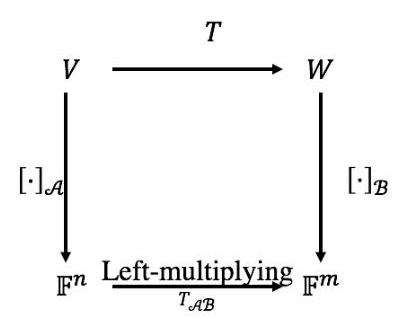
\includegraphics[max width=0.3\textwidth]{images/bo_d1h964v7aajc7382l5mg_45_760_1539_401_319_0.jpg}
\end{center}
\hspace*{3em} 

Figure 3.2: Diagram for the matrix reprentation, where \(n \mathrel{\text{ := }} \dim \left( V\right)\) and \(m \mathrel{\text{ := }} \dim \left( W\right)\)

namely, for any \(v \in  V\),

\[
{\left( T\right) }_{\mathcal{B},\mathcal{A}}{\left( \mathbf{v}\right) }_{\mathcal{A}} = {\left( T\mathbf{v}\right) }_{\mathcal{B}}
\]

Therefore, we can compute \({Tv}\) by matrix multiplication.

Therefore, linear transformation corresponds to coordinate matrix multiplication.

Proof. Suppose \(\mathcal{A} = \left\{  {{\bf v}_1,\ldots ,{\bf v}_n}\right\}\) and \(\mathcal{B} = \left\{  {{\bf w}_1,\ldots ,{\bf w}_n}\right\}\). The proof of this theorem follows the same procedure of that in Theorem (3.1) 1. We show this result for \(\mathbf{v} = {\bf v}_{j}\) first:

\[
\operatorname{LHS} = \left\lbrack  \alpha_{ij}\right\rbrack  {\mathbf{e}}_{j} = \left( \begin{matrix} \alpha_{1j} \\  \vdots \\  \alpha_{nj} \end{matrix}\right)
\]

\[
\mathrm{{RHS}} = {\left( T{\bf v}_{j}\right) }_{\mathcal{B}} = {\left( \mathop{\sum }\limits_{{i = 1}}^{m}\alpha_{ij}{\bf w}_{i}\right) }_{\mathcal{B}} = \left( \begin{matrix} \alpha_{1j} \\  \vdots \\  \alpha_{nj} \end{matrix}\right)
\]

2. Then we show the theorem holds for any \(\mathbf{v} \mathrel{\text{ := }} \mathop{\sum }\limits_{{j = 1}}^n{r}_{j}{\bf v}_{j}\) in \(V\) :

\[
{\left( T\right) }_{\mathcal{B}\mathcal{A}}{\left( \mathbf{v}\right) }_{\mathcal{A}} = {\left( T\right) }_{\mathcal{B}\mathcal{A}}{\left( \mathop{\sum }\limits_{{j = 1}}^n{r}_{j}{\bf v}_{j}\right) }_{\mathcal{A}} \tag{3.8a}
\]

\[
= {\left( T\right) }_{\mathcal{B}\mathcal{A}}\left( {\mathop{\sum }\limits_{{j = 1}}^n{r}_{j}{\left( {\bf v}_{j}\right) }_{\mathcal{A}}}\right)  \tag{3.8b}
\]

\[
= \mathop{\sum }\limits_{{j = 1}}^n{r}_{j}{\left( T\right) }_{\mathcal{B}\mathcal{A}}{\left( {\bf v}_{j}\right) }_{\mathcal{A}} \tag{3.8c}
\]

\[
= \mathop{\sum }\limits_{{j = 1}}^n{r}_{j}{\left( T{\bf v}_{j}\right) }_{\mathcal{B}} \tag{3.8d}
\]

\[
= {\left( \mathop{\sum }\limits_{{j = 1}}^n{r}_{j}\left( T{\bf v}_{j}\right) \right) }_{\mathcal{R}} \tag{3.8e}
\]

\[
= {\left\lbrack  T\left( \mathop{\sum }\limits_{{j = 1}}^n{r}_{j}{\bf v}_{j}\right) \right\rbrack  }_{\mathcal{R}} \tag{3.8f}
\]

\[
= {\left( Tv\right) }_{\mathcal{B}} \tag{3.8g}
\]

The justification for(3.8a)is similar to that shown in Theorem (3.1). The proof is complete.

Consider a special case for Theorem (3.3), i.e., \(T = \mathrm{{id}}\) and \(\mathcal{A},{\mathcal{A}}^{\prime }\) are two ordered basis for the input and output space, respectively. Then the result in Theorem (3.3) implies

\[
{C}_{{\mathcal{A}}^{\prime },\mathcal{A}}{\left( \mathbf{v}\right) }_{\mathcal{A}} = {\left( \mathbf{v}\right) }_{{\mathcal{A}}^{\prime }}
\]

i.e., the matrix representation theorem (3.3) is a general case for the change of basis theorem (3.1)

Proposition 3.6 - Functoriality. Suppose \(V,W,U\) are finite dimensional vector spaces, and let \(\mathcal{A},\mathcal{B},\mathcal{C}\) be the ordered basis for \(V,W,U\), respectively. Suppose that

\[
T : V \rightarrow  W,\;S : W \rightarrow  U
\]

are given two linear transformations, then

\[
{\left( S \circ  T\right) }_{C,\mathcal{A}} = {\left( S\right) }_{C,\mathcal{B}}{\left( T\right) }_{\mathcal{B},\mathcal{A}}
\]

Composition of linear transformation corresponds to the multiplication of change of basis matrices.

Proof. Suppose the ordered basis \(\mathcal{A} = \left\{  {{\bf v}_1,\ldots ,{\bf v}_n}\right\}  ,\mathcal{B} = \left\{  {{\bf w}_1,\ldots ,{\bf w}_{m}}\right\}  ,\mathcal{C} = \left\{  {{\mathbf{u}}_1,\ldots ,{\mathbf{u}}_{p}}\right\}\). By defintion of change of basis matrices,

\[
T\left( {\bf v}_{j}\right)  = \mathop{\sum }\limits_{i}{\left( {T}_{\mathcal{B},\mathcal{A}}\right) }_{ij}{\bf w}_{i}
\]

\[
S\left( {\bf w}_{i}\right)  = \mathop{\sum }\limits_{k}{\left( {S}_{C,\mathcal{B}}\right) }_{ki}{\mathbf{u}}_{k}
\]

\[
{\left( S \circ  T\right) }_{C,\mathcal{A}}{\left( {\bf v}_{j}\right) }_{\mathcal{A}} = {\left( S \circ  T\left( {\bf v}_{j}\right) \right) }_{C} \tag{3.9a}
\]

\[
= {\left\lbrack  S \circ  \left( \mathop{\sum }\limits_{i}{\left( {T}_{\mathcal{B},\mathcal{A}}\right) }_{ij}{\bf w}_{i}\right) \right\rbrack  }_{C} \tag{3.9b}
\]

\[
= \mathop{\sum }\limits_{i}{\left( {T}_{\mathcal{B},\mathcal{A}}\right) }_{ij}{\left( S\left( {\bf w}_{i}\right) \right) }_{\mathcal{C}} \tag{3.9c}
\]

\[
= \mathop{\sum }\limits_{i}{\left( {T}_{\mathcal{B},\mathcal{A}}\right) }_{ij}{\left( \mathop{\sum }\limits_{k}{\left( {S}_{C,\mathcal{B}}\right) }_{ki}{u}_{k}\right) }_{\mathcal{C}} \tag{3.9d}
\]

\[
= \mathop{\sum }\limits_{k}\mathop{\sum }\limits_{i}{\left( {S}_{C,\mathcal{B}}\right) }_{ki}{\left( {T}_{\mathcal{B},\mathcal{A}}\right) }_{ij}{\left( {\mathbf{u}}_{k}\right) }_{\mathcal{C}} \tag{3.9e}
\]

\[
= \mathop{\sum }\limits_{k}{\left( {S}_{C,\mathcal{B}}{T}_{\mathcal{B},\mathcal{A}}\right) }_{kj}{\left( {\mathbf{u}}_{k}\right) }_{C} \tag{3.9f}
\]

\[
= \mathop{\sum }\limits_{k}{\left( {S}_{C,\mathcal{B}}{T}_{\mathcal{B},\mathcal{A}}\right) }_{kj}{\mathbf{e}}_{k} \tag{3.9g}
\]

\[
= j\text{ -th column of }\left\lbrack  {{S}_{C\mathcal{B}}{T}_{\mathcal{B},\mathcal{A}}}\right\rbrack   \tag{3.9h}
\]

where (3.9a) is by the result in theorem (3.3); (3.9b) and (3.9d) follows from definitions of \(T\left( {\bf v}_{j}\right)\) and \(S\left( {\bf w}_{i}\right) ;\left( {{3.9}\mathrm{c}}\right)\) and(3.9e)follows from the linearity of \(C;\left( {{3.9}\mathrm{f}}\right)\) follows from the matrix multiplication definition; (3.9g) is because \({\left( {\mathbf{u}}_{k}\right) }_{C} = {\mathbf{e}}_{k}\).

Therefore, \({\left( S \circ  T\right) }_{C\mathcal{A}}\) and \(\left( {S}_{C,\mathcal{B}}\right) \left( {T}_{\mathcal{B},\mathcal{A}}\right)\) share the same \(j\) -th column, and thus equal to each other.

Corollary 3.2 Suppose that \(S\) and \(T\) are two identity mappings \(V \rightarrow  V\), and consider \({\left( S\right) }_{{\mathcal{A}}^{\prime }\mathcal{A}}\) and \({\left( T\right) }_{\mathcal{A},{\mathcal{A}}^{\prime }}\) in proposition (3.6), then

\[
{\left( S \circ  T\right) }_{{\mathcal{A}}^{\prime },{\mathcal{A}}^{\prime }} = {\left( S\right) }_{{\mathcal{A}}^{\prime }\mathcal{A}}{\left( T\right) }_{\mathcal{A},{\mathcal{A}}^{\prime }}
\]

Therefore,

\[
\text{ Identity matrix } = {C}_{{\mathcal{A}}^{\prime },\mathcal{A}}{C}_{\mathcal{A},{\mathcal{A}}^{\prime }}
\]

Proposition 3.7 Let \(T : V \rightarrow  W\) with \(\dim \left( V\right)  = n,\dim \left( W\right)  = m\), and let

\begin{itemize}
\item \(\mathcal{A},{\mathcal{A}}^{\prime }\) be ordered basis of \(V\)
\end{itemize}

\begin{itemize}
\item \(\mathcal{B},{\mathcal{B}}^{\prime }\) be ordered basis of \(W\)
\end{itemize}

then the change of basis matrices admit the relation

\[
{\left( T\right) }_{{\mathcal{B}}^{\prime },{\mathcal{A}}^{\prime }} = {C}_{{\mathcal{B}}^{\prime },\mathcal{B}}{\left( T\right) }_{\mathcal{B},\mathcal{A}}{C}_{\mathcal{A}{\mathcal{A}}^{\prime }} \tag{3.10}
\]

Here note that \({\left( T\right) }_{{\mathcal{B}}^{\prime },{\mathcal{A}}^{\prime }},{\left( T\right) }_{\mathcal{B},\mathcal{A}} \in  {\mathbb{F}}^{m \times  n};{\mathcal{C}}_{{\mathcal{B}}^{\prime },\mathcal{B}} \in  {\mathbb{F}}^{m \times  m}\) ; and \({\mathcal{C}}_{\mathcal{A}{\mathcal{A}}^{\prime }} \in  {\mathbb{F}}^{n \times  n}\).

Proof. Let \(\mathcal{A} = \left\{  {{\bf v}_1,\ldots ,{\bf v}_n}\right\}  ,{\mathcal{A}}^{\prime } = \left\{  {{\bf v}_1^{\prime },\ldots ,{\bf v}_n^{\prime }}\right\}\). Consider simplifying the \(j\) -th column for the LHS and RHS of (3.10) and showing they are equal:

\[
\text{ LHS } = {\left( T\right) }_{{\mathcal{B}}^{\prime },{\mathcal{A}}^{\prime }}{\mathbf{e}}_{j}
\]

\[
= {\left( T\right) }_{{\mathcal{B}}^{\prime },{\mathcal{A}}^{\prime }}{\left( {\bf v}_{j}^{\prime }\right) }_{{\mathcal{A}}^{\prime }}
\]

\[
= {\left( T{\bf v}_{j}^{\prime }\right) }_{{\mathcal{B}}^{\prime }}
\]

\[
\text{ RHS } = {C}_{{\mathcal{B}}^{\prime },\mathcal{B}}{\left( T\right) }_{\mathcal{B},\mathcal{A}}{C}_{\mathcal{A}{\mathcal{A}}^{\prime }}{\mathbf{e}}_{j}
\]

\[
= {C}_{{\mathcal{B}}^{\prime },\mathcal{B}}{\left( T\right) }_{\mathcal{B},\mathcal{A}}{C}_{\mathcal{A}{\mathcal{A}}^{\prime }}{\left( {\bf v}_{j}^{\prime }\right) }_{{\mathcal{A}}^{\prime }}
\]

\[
= {C}_{{\mathcal{B}}^{\prime },\mathcal{B}}{\left( T\right) }_{\mathcal{B},\mathcal{A}}{\left( {\bf v}_{j}^{\prime }\right) }_{\mathcal{A}}
\]

\[
= {C}_{{\mathcal{B}}^{\prime },\mathcal{B}}{\left( T{\bf v}_{j}^{\prime }\right) }_{\mathcal{B}}
\]

\[
= {\left( T{\bf v}_{j}^{\prime }\right) }_{{\mathcal{B}}^{\prime }}
\]

Let \(T : V \rightarrow  V\) be a linear operator with \(\mathcal{A},{\mathcal{A}}^{\prime }\) being two ordered basisof \(V\), then

\[
{\left( T\right) }_{{\mathcal{A}}^{\prime }{\mathcal{A}}^{\prime }} = {\mathcal{C}}_{{\mathcal{A}}^{\prime },\mathcal{A}}{\left( T\right) }_{\mathcal{A}\mathcal{A}}{\mathcal{C}}_{\mathcal{A},{\mathcal{A}}^{\prime }} = {\left( {\mathcal{C}}_{\mathcal{A},{\mathcal{A}}^{\prime }}\right) }^{-1}{\left( T\right) }_{\mathcal{A}\mathcal{A}}{\mathcal{C}}_{\mathcal{A},{\mathcal{A}}^{\prime }}
\]

Therefore, the change of basis matrices \({\left( T\right) }_{{\mathcal{A}}^{\prime }{\mathcal{A}}^{\prime }}\) and \({\left( T\right) }_{\mathcal{A}\mathcal{A}}\) are similar to each other, which means they share the same eigenvalues, determinant, trace.

Therefore, two similar matrices cooresponds to same linear transformation using different basis.

\section*{Chapter 4}

\section*{Week4}

\section*{4.1. Monday for MAT 3040}

\section*{4.1.1. Quotient Spaces}

Now we aim to divide a big vector space into many pieces of slices.

\begin{itemize}
\item For example, the Cartesian plane can be expressed as union of set of vertical lines
\end{itemize}

as follows:

\[
{\mathbb{R}}^2 = \mathop{\bigcup }\limits_{{m \in  \mathbb{R}}}\left\{  \left( \begin{array}{l} m \\  0 \end{array}\right) \right\}   + \operatorname{span}\{ \left( {0,1}\right) \} \}
\]

\begin{itemize}
\item Another example is that the set of integers can be expressed as union of three sets:
\end{itemize}

\[
\mathbb{Z} = {Z}_1 \cup  {Z}_2 \cup  {Z}_{3}
\]

where \({Z}_{i}\) is the set of integers \(z\) such that \(z{\;\operatorname{mod}\;3} = i\).

Definition 4.1 [Coset] Let \(V\) be a vector space and \(W \leq  V\). For any element \(v \in  V\), the (right) coset determined by \(v\) is the set

\[
\mathbf{v} + W \mathrel{\text{ := }} \{ \mathbf{v} + \mathbf{w} \mid  \mathbf{w} \in  W\}
\]

For example, consider \(V = {\mathbb{R}}^{3}\) and \(W = \operatorname{span}\{ \left( {1,2,0}\right) \}\). Then the coset determined by

\(\mathbf{v} = \left( {5,6, - 3}\right)\) can be written as

\[
v + W = \{ \left( {5 + t,6 + {2t}, - 3}\right)  \mid  t \in  \mathbb{R}\}
\]

It’s interesting that the coset determined by \({\bf v}^{\prime } = \{ \left( {4,4, - 3}\right) \}\) is exactly the same as the coset shown above:

\[
{\bf v}^{\prime } + W = \{ \left( {4 + t,4 + {2t}, - 3}\right)  \mid  t \in  \mathbb{R}\}  = \mathbf{v} + W.
\]

Therefore, write the exact expression of \(\mathbf{v} + W\) may sometimes become tedious and hard to check the equivalence. We say \(v\) is a representative of a coset \(v + W\).

Proposition 4.1 Two cosets are the same iff the subtraction for the corresponding representatives is in \(W\), i.e.,

\[
{\bf v}_1 + W = {\bf v}_2 + W \Leftrightarrow  {\bf v}_1 - {\bf v}_2 \in  W
\]

Proof. Necessity. Suppose that \({\bf v}_1 + W = {\bf v}_2 + W\), then \({\bf v}_1 + {\bf w}_1 = {\bf v}_2 + {\bf w}_2\) for some \({\bf w}_1,{\bf w}_2 \in  W\), which implies

\[
{\bf v}_1 - {\bf v}_2 = {\bf w}_2 - {\bf w}_1 \in  W
\]

Sufficiency. Suppose that \({\bf v}_1 - {\bf v}_2 = \mathbf{w} \in  W\). It suffices to show \({\bf v}_1 + W \subseteq  {\bf v}_2 + W\). For any \({\bf v}_1 + {\bf w}^{\prime } \in  {\bf v}_1 + W\), this element can be expressed as

\[
{\bf v}_1 + {\bf w}^{\prime } = \left( {{\bf v}_2 + \mathbf{w}}\right)  + {\bf w}^{\prime } = {\bf v}_2 + \underset{\text{ belong to }W}{\underbrace{\left( \mathbf{w} + {\bf w}^{\prime }\right) }} \in  {\bf v}_2 + W.
\]

Therefore, \({\bf v}_1 + W \subseteq  {\bf v}_2 + W\). Similarly we can show that \({\bf v}_2 + W \subseteq  {\bf v}_1 + W\).

Exercise: Two cosets with representatives \({\bf v}_1,{\bf v}_2\) have no intersection iff \({\bf v}_1 - {\bf v}_2 \notin  W\).

Definition 4.2 [Quotient Space] The quotient space of \(V\) by the subspace \(W\), is the collection of all cosets \(\mathbf{v} + W\), denoted by \(V/W\).

To make the quotient space a vector space structure, we define the addition and scalar multiplication on \(V/W\) by:

\[
\left( {{\bf v}_1 + W}\right)  + \left( {{\bf v}_2 + W}\right)  \mathrel{\text{ := }} \left( {{\bf v}_1 + {\bf v}_2}\right)  + W
\]

\[
\alpha  \cdot  \left( {\mathbf{v} + W}\right)  \mathrel{\text{ := }} \left( {\alpha  \cdot  \mathbf{v}}\right)  + W
\]

For example, consider \(V = {\mathbb{R}}^2\) and \(W = \operatorname{span}\{ \left( {0,1}\right) \}\). Then note that

\[
\left( {\left( \begin{array}{l} 1 \\  0 \\  0 \end{array}\right)  + W}\right)  + \left( {\left( \begin{array}{l} 2 \\  0 \\  0 \end{array}\right)  + W}\right)  = \left( {\left( \begin{array}{l} 3 \\  0 \\  0 \end{array}\right)  + W}\right)
\]

\[
\pi  \cdot  \left( {\left( \begin{array}{l} 1 \\  0 \end{array}\right)  + W}\right)  = \left( {\left( \begin{array}{l} \pi \\  0 \end{array}\right)  + W}\right)
\]

Proposition 4.2 The addition and scalar multiplication is well-defined.

Proof. 1. Suppose that

\[
\left\{  {\begin{array}{l} {\bf v}_1 + W = {\bf v}_1^{\prime } + W \\  {\bf v}_2 + W = {\bf v}_2^{\prime } + W \end{array},}\right.  \tag{4.1}
\]

and we need to show that \(\left( {{\bf v}_1 + {\bf v}_2}\right)  + W = \left( {{\bf v}_1^{\prime } + {\bf v}_2^{\prime }}\right)  + W\).

From (4.1) and proposition (4.1), we imply

\[
{\bf v}_1 - {\bf v}_1^{\prime } \in  W,\;{\bf v}_2 - {\bf v}_2^{\prime } \in  W
\]

which implies

\[
\left( {{\bf v}_1 - {\bf v}_1^{\prime }}\right)  + \left( {{\bf v}_2 - {\bf v}_2^{\prime }}\right)  = \left( {{\bf v}_1 + {\bf v}_2}\right)  - \left( {{\bf v}_1^{\prime } + {\bf v}_2^{\prime }}\right)  \in  W
\]

By proposition (4.1) again we imply \(\left( {{\bf v}_1 + {\bf v}_2}\right)  + W = \left( {{\bf v}_1^{\prime } + {\bf v}_2^{\prime }}\right)  + W\)

2. For scalar multiplication, similarly, we can show that \({\bf v}_1 + W = {\bf v}_1^{\prime } + W\) implies \(\alpha {\bf v}_1 + W = \alpha {\bf v}_1^{\prime } + W\) for all \(\alpha  \in  \mathbb{F}\).

Proposition 4.3 The canonical projection mapping

\[
{\pi }_{W} : V \rightarrow  V/W
\]

\[
v \mapsto  v + W
\]

is a surjective linear transformation with \(\ker \left( {\pi }_{W}\right)  = W\).

Proof. 1. First we show that \(\ker \left( {\pi }_{W}\right)  = W\) :

\[
{\pi }_{W}\left( \mathbf{v}\right)  = 0 \Rightarrow  \mathbf{v} + W = {\mathbf{0}}_{V/W} \Rightarrow  \mathbf{v} + W = \mathbf{0} + W \Rightarrow  \mathbf{v} = \left( {\mathbf{v} - \mathbf{0}}\right)  \in  W
\]

Here note that the zero element in the quotient space \(V/W\) is the coset with representative 0 .

2. For any \({\bf v}_{0} + W \in  V/W\), we can construct \({\bf v}_{0} \in  V\) such that \({\pi }_{W}\left( {\bf v}_{0}\right)  = {\bf v}_{0} + W\). Therefore the mapping \({\pi }_{W}\) is surjective.

3. To show the mapping \({\pi }_{W}\) is a linear transformation, note that

\[
{\pi }_{W}\left( {\alpha {\bf v}_1 + \beta {\bf v}_2}\right)  = \left( {\alpha {\bf v}_1 + \beta {\bf v}_2}\right)  + W
\]

\[
= \left( {\alpha {\bf v}_1 + W}\right)  + \left( {\beta {\bf v}_2 + W}\right)
\]

\[
= \alpha \left( {{\bf v}_1 + W}\right)  + \beta \left( {{\bf v}_2 + W}\right)
\]

\[
= \alpha {\pi }_{W}\left( {\bf v}_1\right)  + \beta {\pi }_{W}\left( {\bf v}_2\right)
\]

\section*{4.1.2. First Isomorphism Theorem}

The key of linear algebra is to solve the linear system \(\mathbf{{Ax}} = B\) with \(A \in  {\mathbb{R}}^{m \times  n}\). The general step for solving this linear system is as follows:

1. Find the solution set for \(\mathbf{{Ax}} = \mathbf{0}\), i.e., the set \(\ker \left( A\right)\)

2. Find a particular solution \({\mathbf{x}}_{0}\) such that \(A{\mathbf{x}}_{0} = B\).

Then the general solution set to this linear system is \({\mathbf{x}}_{0} + \ker \left( A\right)\), which is a coset in

the space \({\mathbb{R}}^n/\ker \left( A\right)\). Therefore, to solve the linear system \(\mathbf{{Ax}} = B\) suffices to study the quotient space \({\mathbb{R}}^n/\ker \left( A\right)\) :

Proposition 4.4 - Universal Property I. Suppose that \(T : V \rightarrow  W\) is a linear transformation, and that \({V}^{\prime } \leq  \ker \left( T\right)\). Then the mapping

\[
\widetilde{T} : V/{V}^{\prime } \rightarrow  W
\]

\[
\mathbf{v} + {V}^{\prime } \mapsto  T\left( \mathbf{v}\right)
\]

is a well-defined linear transformation. As a result, the diagram below commutes:

\begin{center}
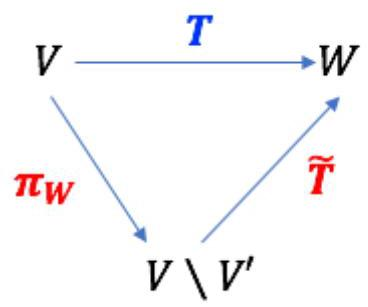
\includegraphics[max width=0.3\textwidth]{images/bo_d1h964v7aajc7382l5mg_55_784_904_368_307_0.jpg}
\end{center}
\hspace*{3em} 

In other words, we have \(T = \widetilde{T} \circ  {\pi }_{W}\).

Proof. First we show the well-definedness. Suppose that \({\bf v}_1 + {V}^{\prime } = {\bf v}_2 + {V}^{\prime }\) and suffices to show \(\widetilde{T}\left( {{\bf v}_1 + {V}^{\prime }}\right)  = \widetilde{T}\left( {{\bf v}_2 + {V}^{\prime }}\right)\), i.e., \(T\left( {\bf v}_1\right)  = T\left( {\bf v}_2\right)\). By proposition (4.1), we imply

\[
{\bf v}_1 - {\bf v}_2 \in  {V}^{\prime } \leq  \ker \left( T\right)  \Rightarrow  T\left( {{\bf v}_1 - {\bf v}_2}\right)  = \mathbf{0} \Rightarrow  T\left( {\bf v}_1\right)  - T\left( {\bf v}_2\right)  = \mathbf{0}.
\]

Then we show \(\widetilde{(}T)\) is a linear transformation:

\[
\widetilde{T}\left( {\alpha \left( {{\bf v}_1 + {V}^{\prime }}\right)  + \beta \left( {{\bf v}_2 + {V}^{\prime }}\right) }\right)  = \widetilde{T}\left( {\left( {\alpha {\bf v}_1 + \beta {\bf v}_2}\right)  + {V}^{\prime }}\right)
\]

\[
= T\left( {\alpha {\bf v}_1 + \beta {\bf v}_2}\right)
\]

\[
= {\alpha T}\left( {\bf v}_1\right)  + {\beta T}\left( {\bf v}_2\right)
\]

\[
= \alpha \widetilde{T}\left( {{\bf v}_1 + {V}^{\prime }}\right)  + \beta \widetilde{T}\left( {{\bf v}_2 + {V}^{\prime }}\right)
\]

Actually, if we let \({V}^{\prime } = \ker \left( T\right)\), the mapping \(\widetilde{T} : V/{V}^{\prime } \rightarrow  T\left( V\right)\) forms an isomorphism, In particular, if further \(T\) is surjective, then \(T\left( V\right)  = W\), i.e., the mapping \(\widetilde{T} : V/{V}^{\prime } \rightarrow  W\) forms an isomorphism.

Theorem 4.1 - First Isomorphism Theorem. Let \(T : V \rightarrow  W\) be a surjective linear transformation. Then the mapping

\[
\widetilde{T} : V/\ker \left( T\right)  \rightarrow  W
\]

\[
v + \ker \left( T\right)  \mapsto  T\left( v\right)
\]

is an isomorphism.

Proof. Injectivity. Suppose that \(\widetilde{T}\left( {{\bf v}_1 + \ker \left( T\right) }\right)  = \widetilde{T}\left( {{\bf v}_2 + \ker \left( T\right) }\right)\), then we imply

\[
T\left( {\bf v}_1\right)  = T\left( {\bf v}_2\right)  \Rightarrow  T\left( {{\bf v}_1 - {\bf v}_2}\right)  = {\mathbf{0}}_{W} \Rightarrow  {\bf v}_1 - {\bf v}_2 \in  \ker \left( T\right) ,
\]

i.e., \({\bf v}_1 + \ker \left( T\right)  = {\bf v}_2 + \ker \left( T\right)\).

Surjectivity. For \(w \in  W\), due to the surjectivity of \(T\), we can find a \({\bf v}_{0}\) such that \(T\left( {\bf v}_{0}\right)  = \mathbf{w}\). Therefore, we can construct a set \({\bf v}_{0} + \ker \left( T\right)\) such that

\[
\widetilde{T}\left( {{\bf v}_{0} + \ker \left( T\right) }\right)  = \mathbf{w}.
\]

\section*{4.4. Wednesday for MAT 3040}

Reviewing.

\begin{itemize}
\item Quotient Space:
\end{itemize}

\[
V/W = \{ \mathbf{v} + W \mid  \mathbf{v} \in  V\}
\]

The elements in \(V/W\) are cosets. Note that \(V/W\) does not mean a subset of \(V\).

\begin{itemize}
\item Define the canonical projection mapping
\end{itemize}

\[
{\pi }_{W} : V \rightarrow  V/W
\]

\[
\text{ with }\mathbf{v} \mapsto  \mathbf{v} + W\text{ , }
\]

then we imply \({\pi }_{W}\) is a surjective linear transformation with \(\ker \left( {\pi }_{W}\right)  = W\).

If \(\dim \left( V\right)  < \infty\), then by Rank-Nullity Theorem (2.3), we imply that

\[
\dim \left( V\right)  = \dim \left( W\right)  + \dim \left( {V/W}\right)
\]

i.e., \(\dim \left( {V/W}\right)  = \dim \left( V\right)  - \dim \left( W\right)\).

\begin{itemize}
\item (Universal Property I) Every linear transformation \(T : V \rightarrow  W\) with \({V}^{\prime } \leq  \ker \left( T\right)\) can be descended to the composition of the canonical projection mapping \({\pi }_{{V}^{\prime }}\) and the mapping
\end{itemize}

\[
\widetilde{T} : V/{V}^{\prime } \rightarrow  W
\]

\[
\text{ with }\mathbf{v} + {V}^{\prime } \mapsto  T\left( \mathbf{v}\right) \text{ . }
\]

In other words, the diagram (2.1) commutes:

\begin{center}
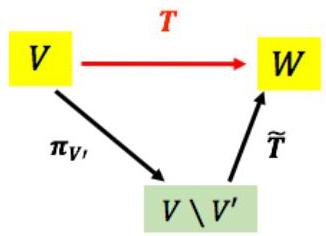
\includegraphics[max width=0.2\textwidth]{images/bo_d1h964v7aajc7382l5mg_57_667_1785_326_236_0.jpg}
\end{center}
\hspace*{3em} 

Diagram (2.1)

In other words, the mapping starting from either the black or red line gives the same result, i.e., \(T\left( \mathbf{v}\right)  = \widetilde{T} \circ  {\pi }_{{V}^{\prime }}\left( \mathbf{v}\right)  = \widetilde{T}\left( {\mathbf{v} + {V}^{\prime }}\right)\) for any \(\mathbf{v} \in  V\).

\begin{itemize}
\item (First Isomorphism Theorem) Under the setting of Universal Property I (UPI), if \(T\) is a surjective linear transformation with \({V}^{\prime } = \ker \left( T\right)\), then the \(\widetilde{T}\) is an isomorphism.
\end{itemize}

\begin{itemize}
\item Example 4.2 Suppose that \(U,W \leq  V\) with \(U \cap  W = \{ \mathbf{0}\}\), then define the mapping
\end{itemize}

\[
\phi  : U \oplus  W \rightarrow  U
\]

\[
\text{ with }\phi \left( {\mathbf{u} + \mathbf{w}}\right)  = \mathbf{u}
\]

Exercise: if \(U,W \leq  V\) but \(U \cap  W \neq  \{ \mathbf{0}\}\), then the mapping

\[
\phi  : U + W \rightarrow  U
\]

is not well-defined:

\[
\text{ with }\mathbf{u} + \mathbf{w} \mapsto  \mathbf{u}
\]

Suppose that \(\mathbf{0} \neq  \mathbf{v} \in  U \cap  W\) and for any \(\mathbf{u} \in  U,\mathbf{w} \in  W\), we construct

\[
{\mathbf{u}}^{\prime } = \mathbf{u} - \mathbf{v} \in  U,\;{\bf w}^{\prime } = \mathbf{w} + \mathbf{v} \in  V \Rightarrow  \phi \left( {{\mathbf{u}}^{\prime } + {\bf w}^{\prime }}\right)  = \mathbf{u} - \mathbf{v}
\]

Therefore we get \(\mathbf{u} + \mathbf{w} = {\mathbf{u}}^{\prime } + {\bf w}^{\prime }\) but \(\phi \left( {\mathbf{u} + \mathbf{w}}\right)  \neq  \phi \left( {{\mathbf{u}}^{\prime } + {\bf w}^{\prime }}\right)\).

Back to the situation \(U \cap  W = \{ \mathbf{0}\}\), then it’s clear that \(\phi  : U \oplus  W \rightarrow  U\) is surjective linear transformation with \(\ker \left( \phi \right)  = W\). Therefore, construct the new mapping

\[
\widetilde{\phi } : U \oplus  W/W \rightarrow  U
\]

\[
\text{ with }\mathbf{u} + \mathbf{w} + W \mapsto  \phi \left( {\mathbf{u} + \mathbf{w}}\right)
\]

We imply \(\widetilde{\phi }\) is an isomorphism by First Isomorphism Theorem.

Now we study the generalized quotients, which is defined to satisfy the generalized version of universal property I.

Definition 4.7 [Universal Property for Quotients] Let \(V\) be a vector space and \({V}^{\prime } \leq  V\). Consider the collection of linear transformations

\[
\mathrm{{Obj}} = \left\{  {T : V \rightarrow  W\left| {\;\begin{array}{l} T\text{ is a linear transformation } \\  {V}^{\prime } \leq  \ker \left( T\right)  \end{array}}\right. }\right\}
\]

(For example, \({\pi }_{{V}^{\prime }} : V \rightarrow  V/{V}^{\prime }\) is an element from the set Obj.)

An element \(\left( {\phi  : V \rightarrow  U}\right)  \in  \mathrm{{Obj}}\) is said to satisfy the universal property if it satisfies the following:

Given any element \(\left( {T : V \rightarrow  W}\right)  \in  \mathrm{{Obj}}\), we can extend the transformation \(\phi\) with a uniquely existing \(\widetilde{T} : U \rightarrow  W\) so that the diagram (2.2) commutes:

\begin{center}
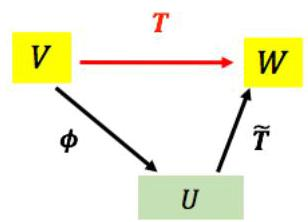
\includegraphics[max width=0.2\textwidth]{images/bo_d1h964v7aajc7382l5mg_59_650_1012_308_222_0.jpg}
\end{center}
\hspace*{3em} 

Diagram (2.2)

Or equivalently, for given \(\left( {T : V \rightarrow  W}\right)  \in  \mathrm{{Obj}}\), there exists the unique mapping \(\widetilde{T} : U \rightarrow  W\) such that \(T = \widetilde{T} \circ  \phi\).

Theorem 4.3 - Universal Property II. 1. The mapping \(\left( {{\pi }_{{V}^{\prime }} : V \rightarrow  V/{V}^{\prime }}\right)  \in\) Obj is a universal object, i.e., it satisfies the universal property.

2. If \(\left( {\phi  : V \rightarrow  U}\right)\) is a universal object, then \(U \cong  V/{V}^{\prime }\), i.e., there is intrinsically "one" element in the set of universal objects.

Proof. 1. Consider any linear transformation \(T : V \rightarrow  W\) such that \({V}^{\prime } \leq  \ker \left( T\right)\), then define (construct) the same \(\widetilde{T} : V/{V}^{\prime } \rightarrow  W\) as that in UPI. Therefore, for given \(T\), applying the result of UPI, we imply \(T = \widetilde{T} \circ  {\pi }_{{V}^{\prime }}\), i.e., \({\pi }_{{V}^{\prime }}\) satisfies the diagram (2.2).

To show the uniqueness of \(\widetilde{T}\), suppose there exists \(\widetilde{S} : V/{V}^{\prime } \rightarrow  W\) such that the diagram (2.3) commutes.

\begin{center}
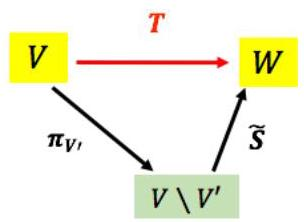
\includegraphics[max width=0.2\textwidth]{images/bo_d1h964v7aajc7382l5mg_60_806_519_304_222_0.jpg}
\end{center}
\hspace*{3em} 

Diagram (2.3)

It suffices to show the mapping \(\widetilde{S} = \widetilde{T}\) : for any \(v + {V}^{\prime } \in  V/{V}^{\prime }\), we have

\[
\widetilde{S}\left( {\mathbf{v} + {V}^{\prime }}\right)  \mathrel{\text{ := }} \widetilde{S} \circ  {\pi }_{{V}^{\prime }}\left( \mathbf{v}\right)  = T\left( \mathbf{v}\right) ,
\]

where the first equality is due to the surjectivity of \({\pi }_{{V}^{\prime }}\). By the result of UPI, \(T\left( \mathbf{v}\right)  = \widetilde{T}\left( {\mathbf{v} + {V}^{\prime }}\right)\). Therefore \(\widetilde{T}\left( {\mathbf{v} + {V}^{\prime }}\right)  = \widetilde{S}\left( {\mathbf{v} + {V}^{\prime }}\right)\) for all \(\mathbf{v} + {V}^{\prime } \in  V/{V}^{\prime }\). The proof is complete.

2. Suppose that \(\left( {\phi  : V \rightarrow  U}\right)\) satisfies the universal property. In particular, the following two diagrams hold:

\begin{center}
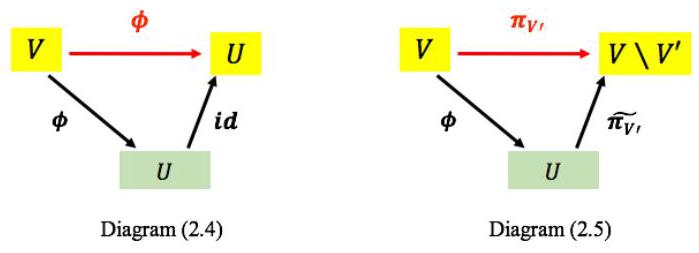
\includegraphics[max width=0.5\textwidth]{images/bo_d1h964v7aajc7382l5mg_60_604_1592_699_253_0.jpg}
\end{center}
\hspace*{3em} 

Since \(\left( {\pi }_{{V}^{\prime }}\right)\) satisfies the universal property, in particular, the following two diagrams hold:

\begin{center}
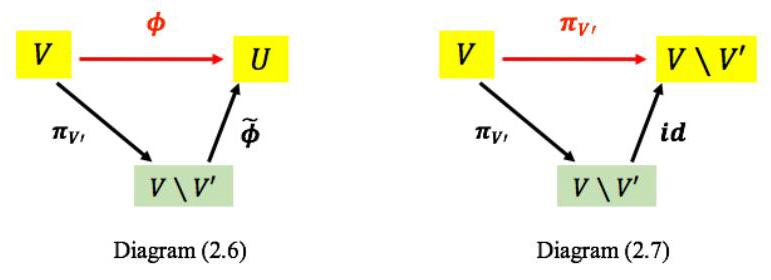
\includegraphics[max width=0.6\textwidth]{images/bo_d1h964v7aajc7382l5mg_61_446_336_771_280_0.jpg}
\end{center}
\hspace*{3em} 

Then we claim that: Combining Diagram (2.5) and (2.6), we imply the diagram (2.8):

\begin{center}
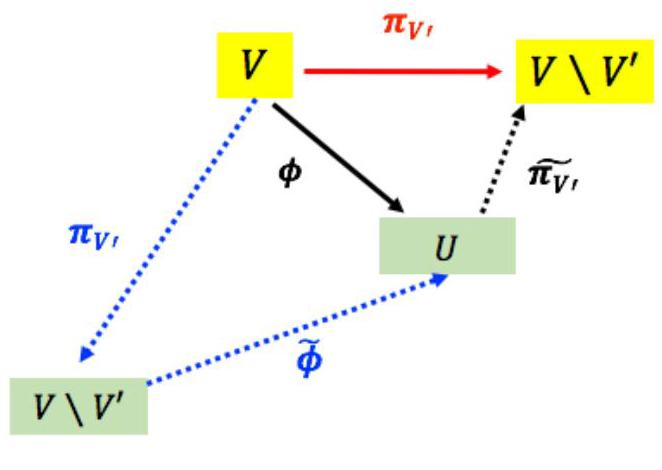
\includegraphics[max width=0.5\textwidth]{images/bo_d1h964v7aajc7382l5mg_61_444_1118_662_470_0.jpg}
\end{center}
\hspace*{3em} 

Diagram (2.8)

Graph Description: Note that this diagram commutes, i.e., the mapping starting from either the red line or the dash line gives the same result, i.e., \({\pi }_{{V}^{\prime }} = {\widetilde{\pi }}_{{V}^{\prime }} \circ  \widetilde{\phi } \circ  {\pi }_{{V}^{\prime }}\). Comparing Diagram (2.7) and Diagram (2.8), we have \({\widetilde{\pi }}_{{V}^{\prime }} \circ  \widetilde{\phi } = {id}\), by the uniqueness of the universal object.

Therefore, \({\widetilde{\pi }}_{{V}^{\prime }} \circ  \widetilde{\phi } = {id}\) implies \({\widetilde{\pi }}_{{V}^{\prime }}\) is surjective and \(\widetilde{\phi }\) is injective.

Also, combining Diagram (2.6) and (2.5), we imply diagram (2.9):

\begin{center}
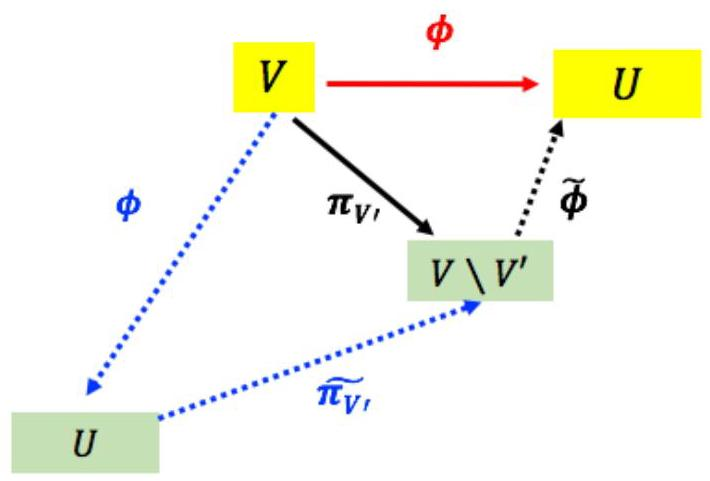
\includegraphics[max width=0.6\textwidth]{images/bo_d1h964v7aajc7382l5mg_62_611_342_710_481_0.jpg}
\end{center}
\hspace*{3em} 

Diagram (2.9)

Graph Description: Note that this diagram commutes, i.e., the mapping starting from either the red line or the dash line gives the same result, i.e., \(\phi  = \widetilde{\phi } \circ  {\widetilde{\pi }}_{{V}^{\prime }} \circ  \phi\). Comparing Diagram (2.9) and Diagram (2.4), we have \(\widetilde{\phi } \circ  {\widetilde{\pi }}_{{V}^{\prime }} = {id}\), by the uniqueness of the universal object

Therefore, \(\widetilde{\phi } \circ  {\widetilde{\pi }}_{{V}^{\prime }} = {id}\) implies \(\widetilde{\phi }\) is surjective and \({\widetilde{\pi }}_{{V}^{\prime }}\) is injective.

Therefore, both \(\widetilde{\phi } : U \rightarrow  V/{V}^{\prime }\) and \({\widetilde{\pi }}_{{V}^{\prime }} : V/{V}^{\prime } \rightarrow  U\) are bijective, i.e., \(U \cong  V/{V}^{\prime }\). The proof is complete.

\section*{4.4.1. Dual Space}

Definition 4.8 Let \(V\) be a vector space over a field \(\mathbb{F}\). The dual vector space \({V}^{ * }\) is defined as

\[
{V}^{ * } = {\operatorname{Hom}}_{\mathbb{F}}\left( {V,\mathbb{F}}\right)
\]

\[
= \{ f : V \rightarrow  \mathbb{F} \mid  f\text{ is a linear transformation }\}
\]

1. Consider \(V = {\mathbb{R}}^n\) and define \({\phi }_{i} : V \rightarrow  \mathbb{R}\) as the \(i\) -th component of

input:

\[
{\phi }_{i}\left( \begin{matrix} {x}_1 \\  \vdots \\  {x}_n \end{matrix}\right)  = {x}_{i}
\]

Then we imply \({\phi }_{i} \in  {V}^{ * }\). On the contrary, \({\phi }_{i}^2\left( \begin{matrix} {x}_1 \\  \vdots \\  {x}_n \end{matrix}\right)  = {x}_{i}^2\) is not in \({V}^{ * }\)

2. Consider \(V = \mathbb{F}\left\lbrack  x\right\rbrack\) and define \(\phi  : V \rightarrow  \mathbb{F}\) as:

\[
\phi \left( {p\left( x\right) }\right)  = p\left( 1\right) ,
\]

It’s clear that \(\phi  \in  {V}^{ * }\) :

\[
\phi \left( {{ap}\left( x\right)  + {bq}\left( x\right) }\right)  = {ap}\left( 1\right)  + {bq}\left( 1\right)
\]

\[
= {a\phi }\left( {p\left( x\right) }\right)  + {b\phi }\left( {q\left( x\right) }\right)
\]

3. Also, \(\psi  : V \rightarrow  \mathbb{F}\) by \(\psi \left( {p\left( x\right) }\right)  = {\int }_{0}^1p\left( x\right) \mathrm{d}x\) is in \({V}^{ * }\).

4. Also, for \(V = {M}_{n \times  n}\left( \mathbb{F}\right)\), the mapping \(\operatorname{tr} : V \rightarrow  \mathbb{F}\) by \(\operatorname{tr}\left( M\right)  = \mathop{\sum }\limits_{{i = 1}}^n{M}_{ii}\) is in \({V}^{ * }\). However, the det : \(V \rightarrow  \mathbb{F}\) is not in \({V}^{ * }\)

Definition 4.9 Let \(V\) be a vector space, with basis \(B = \left\{  {{\bf v}_{i} \mid  i \in  I}\right\}  (I\) can be finite or countable, or uncountable). Define

\[
{B}^{ * } = \left\{  {{f}_{i} : V \rightarrow  \mathbb{F} \mid  i \in  I}\right\}  ,
\]

where \({f}_{i}\) ’s are defined on the basis \(B\) :

\[
{f}_{i}\left( {\bf v}_{j}\right)  = {\delta }_{ij} = \left\{  \begin{array}{ll} 1, & \text{ if }i = j \\  0, & \text{ if }i \neq  j \end{array}\right.
\]

Then we extend \({f}_{i}\) ’s linearly, i.e., for \(\mathop{\sum }\limits_{{j = 1}}^n\alpha_{j}{\bf v}_{j} \in  V\),

\[
{f}_{i}\left( {\mathop{\sum }\limits_{{j = 1}}^n\alpha_{j}{\bf v}_{j}}\right)  = \mathop{\sum }\limits_{{i = 1}}^n\alpha_{j}{f}_{i}\left( {\bf v}_{j}\right) .
\]

It’s clear that \({f}_{i} \in  {V}^{ * }\) is well-defined.

Our question is that whether the \({B}^{ * }\) can be the basis of \({V}^{ * }\) ?

\section*{Chapter 5}

\section*{Week5}

\section*{5.1. Monday for MAT 3040}

Reviewing.

\begin{itemize}
\item Dual space: the set of linear transformations from \(V\) to \(\mathbb{F}\), denoted as \(\operatorname{Hom}\left( {V,\mathbb{F}}\right)\).
\end{itemize}

\begin{itemize}
\item Suppose \(B = \left\{  {{\bf v}_{i} \mid  i \in  I}\right\}\) is the basis of \(V\), define \({B}^{ * } = \left\{  {{f}_{i} \mid  i \in  I}\right\}\) by
\end{itemize}

\[
{f}_{i}\left( {\bf v}_{j}\right)  = {\delta }_{ij} = \left\{  \begin{array}{ll} 1, & i = j \\  0, & i \neq  j \end{array}\right.
\]

Actually, the above recipe uniquely defines a linear transformation \({f}_{i} : V \rightarrow  \mathbb{F}\) : For any \(\mathbf{v} \in  V\), it can be written as \(\mathbf{v} = \mathop{\sum }\limits_{{i \in  I}}\alpha_{i}{\bf v}_{i}\), and therefore

\[
{f}_{i}\left( \mathbf{v}\right)  = {f}_{i}\left( {\mathop{\sum }\limits_{{i \in  I}}\alpha_{i}{\bf v}_{i}}\right)  = \mathop{\sum }\limits_{{i \in  I}}\alpha_{i}{f}_{i}\left( {\bf v}_{i}\right) .
\]

\begin{itemize}
\item Example 5.1 Consider \(V = {\mathbb{R}}^n,B = \left\{  {{\mathbf{e}}_1,\ldots ,{\mathbf{e}}_n}\right\}\). Then we imply \({B}^{ * } = {\left\{  {\phi }_{i}\right\}  }_{i = 1}^n\), where \({\phi }_{i}\) is the mapping \(V \rightarrow  \mathbb{R}\) defined by
\end{itemize}

\[
{\phi }_{i}\left( \begin{matrix} {x}_1 \\  \vdots \\  {x}_n \end{matrix}\right)  = \phi \left( {{x}_1{\mathbf{e}}_1 + \cdots  + {x}_n{\mathbf{e}}_n}\right)  = \mathop{\sum }\limits_{{j = 1}}^n{x}_{j}{\phi }_{i}\left( {\mathbf{e}}_{j}\right)  = {x}_{i}
\]

\section*{5.1.1. Remarks on Dual Space}

Proposition 5.1 1. \({B}^{ * }\) is always lienarly independent, i.e., any finite subset of \({B}^{ * }\) is linearly independent.

2. If \(V\) has finite dimension, then \({B}^{ * }\) is a basis of \({V}^{ * }\).

Proof. 1. Suppose that

\[
\alpha_1{f}_{{i}_1} + \alpha_2{f}_{{i}_2} + \cdots  + \alpha_{k}{f}_{{i}_{k}} = {\mathbf{0}}_{{V}^{ * }}.
\]

In particular, let the input of these linear transformations be \({\bf v}_{{i}_1}\), we imply

\[
\alpha_1{f}_{{i}_1}\left( {\bf v}_{{i}_1}\right)  + \alpha_2{f}_{{i}_2}\left( {\bf v}_{{i}_1}\right)  + \cdots  + \alpha_{k}{f}_{{i}_{k}}\left( {\bf v}_{{i}_1}\right)  = \mathbf{0}\left( {\bf v}_{{i}_1}\right)  \equiv  \mathbf{0}
\]

\[
= \alpha_1 \cdot  1 + \cdots  + 0
\]

\[
= \alpha_1
\]

Applying the same trick, one can show that \(\alpha_2 = \cdots  = \alpha_{k} = 0\). Therefore, \(\left\{  {{f}_{{i}_1},\ldots ,{f}_{{i}_{k}}}\right\}\) is linearly independent.

2. Suppose that \(B = \left\{  {{\bf v}_1,\ldots ,{\bf v}_n}\right\}\) and \({B}^{ * } = \left\{  {{f}_1,\ldots ,{f}_n}\right\}\). For any \(f \in  {V}^{ * }\), construct the linear transformation

\[
g \mathrel{\text{ := }} \mathop{\sum }\limits_{{i = 1}}^nf\left( {\bf v}_{i}\right)  \cdot  {f}_{i} \in  \operatorname{span}\left\{  {B}^{ * }\right\}  .
\]

It follows that for \(j = 1,2,\ldots ,n\),

\[
g\left( {\bf v}_{j}\right)  = \mathop{\sum }\limits_{{i = 1}}^nf\left( {\bf v}_{i}\right)  \cdot  {f}_{i}\left( {\bf v}_{j}\right)  = f\left( {\bf v}_{j}\right) .
\]

It’s clear that \(g\left( \mathbf{v}\right)  = f\left( \mathbf{v}\right)\) for all \(\mathbf{v} \in  V\), i.e., \(f \equiv  g \in  \operatorname{span}\left( {B}^{ * }\right)\). Therefore \({B}^{ * }\) spans \({V}^{ * }\), i.e., forms a basis of \({V}^{ * }\).

Corollary 5.1 If \(\dim \left( V\right)  = n\), then \(\dim \left( {V}^{ * }\right)  = n\).

Proof. It's eay to show the mapping defined as

\[
V \rightarrow  {V}^{ * }
\]

\[
\text{ with }{\bf v}_{i} \mapsto  {f}_{i}
\]

is an isomorphism from \(V \rightarrow  {V}^{ * }\). Note that this constructed isomorphism depends on the choice of basis \(B\) in \(V\). (We say this is not a natural isomorphism.)

R The part 2 for proposition (5.1) does not hold for \(V\) with infinite dimension. The reason is that the spanning set is defined with finite linear combinations. Check the example below for a counter-example.

\begin{itemize}
\item Example 5.2 Suppose that \(V = \mathbb{F}\left\lbrack  x\right\rbrack\), and \({B}^{ * } = \left\{  {1,x,{x}^2,\ldots ,}\right\}\) forms a basis of \(V\). We imply that \({B}^{ * } = \left\{  {{\phi }_{0},{\phi }_1,{\phi }_2,\ldots }\right\}\), where \({\phi }_{i}\) is the mapping defined as
\end{itemize}

\[
{\phi }_{i}\left( {x}^{j}\right)  = \left\{  \begin{array}{ll} 1, & i = j \\  0, & \text{ otherwise } \end{array}\right.
\]

Consider a special element \(\phi  \in  {V}^{ * }\) with \(f\left( {p\left( x\right) }\right)  = p\left( 1\right)\) :

\[
\phi \left( 1\right)  = 1,\;\phi \left( x\right)  = 1,\;\phi \left( {x}^2\right)  = 1,\;\cdots \;\phi \left( {x}^n\right)  = 1,\;\forall n \in  \mathbb{N}.
\]

If following the proof in proposition (5.1), we expect that

\[
g \mathrel{\text{ := }} \mathop{\sum }\limits_{{n = 0}}^{\infty }\phi \left( {x}^n\right) {\phi }_n = \mathop{\sum }\limits_{{n = 0}}^{\infty }{\phi }_n \in  \operatorname{span}\left\{  {B}^{ * }\right\}  ,
\]

which is a contradiction, since \(\operatorname{span}\left\{  {B}^{ * }\right\}\) consists of finite sum of \({\phi }_{i}\) ’s only.

Therefore, if \(V\) is not finite-dimensional, we can say the cardinality of \(V\) is strictly less than the cardinality of \({V}^{ * }\).

Any subspace of a given vector space has some gap. Now we want to describe this gap formally from the perspective of the dual space.

\section*{5.1.2. Annihilators}

Definition 5.1 Let \(V\) be a vector space, \(S \subseteq  V\) be a subset. The annihilator of \(S\) is

defined as

\[
\operatorname{Ann}\left( S\right)  = \left\{  {f \in  {V}^{ * } \mid  f\left( s\right)  = 0,\forall s \in  S}\right\}
\]

\begin{itemize}
\item Example 5.3 Consider \(V = {\mathbb{R}}^{4},B = \left\{  {{\mathbf{e}}_1,\ldots ,{\mathbf{e}}_{4}}\right\}\). Let \({B}^{ * } = \left\{  {{f}_1,\ldots ,{f}_{4}}\right\}  ,S = \left\{  {{\mathbf{e}}_{3},{\mathbf{e}}_{4}}\right\}\).
\end{itemize}

\begin{itemize}
\item Then \({f}_1 \in  \operatorname{Ann}\left( S\right)\), since
\end{itemize}

\[
{f}_1\left( {\mathbf{e}}_{3}\right)  = 0,\;{f}_1\left( {\mathbf{e}}_{4}\right)  = 0
\]

Indeed, any \(a \cdot  {f}_1 + b \cdot  {f}_2 \in  {V}^{ * }\) is in \(\operatorname{Ann}\left( S\right)\).

Proposition 5.2 1. The set \(\operatorname{Ann}\left( S\right)\) is a vector subspace of \({V}^{ * }\)

2. The mapping \(\operatorname{Ann}\left( \cdot \right)\) is inclusion-reversing, i.e., if \({\bf w}_1 \subseteq  {\bf w}_2 \subseteq  V\), then

\[
\operatorname{Ann}\left( {\bf w}_1\right)  \supseteq  \operatorname{Ann}\left( {\bf w}_2\right)
\]

3. The mapping \(\operatorname{Ann}\left( \cdot \right)\) is idempotent, i.e., \(\operatorname{Ann}\left( S\right)  = \operatorname{Ann}\left( {\operatorname{span}\left( S\right) }\right)\).

4. If \(V\) has finite dimension, and \(W \leq  V\), then \(\operatorname{Ann}\left( W\right)\) fills in the gap, i.e.,

\[
\dim \left( W\right)  + \dim \left( {\operatorname{Ann}\left( W\right) }\right)  = \dim \left( V\right)
\]

Proof. 1. Suppose that \(f,g \in  \operatorname{Ann}\left( S\right)\), i.e., \(f\left( s\right)  = g\left( s\right)  = 0,\forall s \in  S\). It’s clear that \(({af} +\)  \({bg}) \in  \operatorname{Ann}\left( S\right)\).

2. Suppose that \(f \in  \operatorname{Ann}\left( {\bf w}_2\right)\), we imply \(f\left( \mathbf{w}\right)  = 0\) for any \(\mathbf{w} \in  {\bf w}_2\). Therefore, \(f\left( {\bf w}_1\right)  = 0\) for any \({\bf w}_1 \in  {\bf w}_1 \subseteq  {\bf w}_2\), i.e., \(f \in  \operatorname{Ann}\left( {\bf w}_1\right)\).

3. Note that \(S \subseteq  \operatorname{span}\left( S\right)\). Therefore we imply \(\operatorname{Ann}\left( S\right)  \supseteq  \operatorname{Ann}\left( {\operatorname{span}\left( S\right) }\right)\) from part(b). It suffices to show \(\operatorname{Ann}\left( S\right)  \subseteq  \operatorname{Ann}\left( {\operatorname{span}\left( S\right) }\right)\) :

For any \(f \in  \operatorname{Ann}\left( S\right)\) and any \(\mathop{\sum }\limits_{{i = 1}}^n{k}_{i}{\mathbf{s}}_{i} \in  \operatorname{span}\left( S\right)\), we imply

\[
f\left( {\mathop{\sum }\limits_{{i = 1}}^n{k}_{i}{\mathbf{s}}_{i}}\right)  = \mathop{\sum }\limits_{{i = 1}}^n{k}_{i}f\left( {\mathbf{s}}_{i}\right)
\]

\[
= \mathop{\sum }\limits_{{i = 1}}^n{k}_{i} \cdot  0
\]

\[
= 0\text{ , }
\]

i.e., \(f \in  \operatorname{Ann}\left( {\operatorname{span}\left( S\right) }\right)\).

4. Let \(\left\{  {{\bf v}_1,\ldots ,{\bf v}_{k}}\right\}\) be a basis of \(W\). By basis extension, we construct a basis of \(V\) :

\[
B = \left\{  {{\bf v}_1,\ldots ,{\bf v}_{k},{\bf v}_{k + 1},\ldots ,{\bf v}_n}\right\}  .
\]

Let \({B}^{ * } = \left\{  {{f}_1,\ldots ,{f}_{k},{f}_{k + 1},\ldots ,{f}_n}\right\}\) be a basis of \({V}^{ * }\). We claim that \(\left\{  {{f}_{k + 1},\ldots ,{f}_n}\right\}\) is a basis of \(\operatorname{Ann}\left( W\right)\) :

\begin{itemize}
\item Firstly, \({f}_{j}\) ’s are the elements in \(\operatorname{Ann}\left( W\right)\) for \(j = k + 1,\ldots ,n\), since for any \(\mathbf{w} = \mathop{\sum }\limits_{{i = 1}}^{k}\alpha_{i}\left( {\bf v}_{i}\right)  \in  W\), we have
\end{itemize}

\[
{f}_{j}\left( \mathbf{w}\right)  = \mathop{\sum }\limits_{{i = 1}}^{k}\alpha_{i}{f}_{j}\left( {\bf v}_{i}\right)
\]

\[
= \mathop{\sum }\limits_{{i = 1}}^{k}\alpha_{i} \cdot  0
\]

\[
= 0,\;j = k + 1,k + 2,\ldots ,n
\]

\begin{itemize}
\item Secondly, the set \(\left\{  {{f}_{k + 1},\ldots ,{f}_n}\right\}\) is linearly independent, since the set \({B}^{ * } =\)  \(\left\{  {{f}_1,\ldots ,{f}_n}\right\}\) is linearly independent.
\end{itemize}

\begin{itemize}
\item Thirdly, \(\left\{  {{f}_{k + 1},\ldots ,{f}_n}\right\}\) spans \(\operatorname{Ann}\left( W\right)\) : for any \(g \in  \operatorname{Ann}\left( W\right)  \subseteq  {V}^{ * }\), it can be
\end{itemize}

expressed as \(g = \mathop{\sum }\limits_{{i = 1}}^n\beta_{i}{f}_{i}\). It follows that

\[
g\left( {\bf v}_1\right)  = \mathop{\sum }\limits_{{i = 1}}^n\beta_{i}{f}_{i}\left( {\bf v}_1\right)  = 0 \Rightarrow  \beta_1 = 0
\]

\[
g\left( {\bf v}_{k}\right)  = \mathop{\sum }\limits_{{i = 1}}^n\beta_{i}{f}_{i}\left( {\bf v}_{k}\right)  = 0 \Rightarrow  \beta_{k} = 0
\]

Substituting \(\beta_1 = \cdots  = \beta_{k} = 0\) into \(g = \mathop{\sum }\limits_{{i = 1}}^n\beta_{i}{f}_{i}\), we imply

\[
g = \beta_{k + 1}{f}_{k + 1} + \cdots  + \beta_n{f}_n \in  \operatorname{span}\left\{  {{f}_{k + 1},\ldots ,{f}_n}\right\}  .
\]

Therefore, \(\left\{  {{f}_{k + 1},\ldots ,{f}_n}\right\}\) forms a basis for \(\operatorname{Ann}\left( W\right)\), i.e., \(\dim \left( {\operatorname{Ann}\left( W\right) }\right)  = n - k\).

Let \(W \leq  V\), where \(V\) has finite dimension, recall that we have obtained two relations below:

\[
\dim \left( {\operatorname{Ann}\left( W\right) }\right)  = \dim \left( V\right)  - \dim \left( W\right)
\]

\[
\dim \left( {\left( V/W\right) }^{ * }\right)  = \dim \left( {V/W}\right)  = \dim \left( V\right)  - \dim \left( W\right)
\]

Therefore, \(\dim \left( {\left( V/W\right) }^{ * }\right)  = \dim \left( {\operatorname{Ann}\left( W\right) }\right)\), i.e.,

\[
{\left( V/W\right) }^{ * } \cong  \operatorname{Ann}\left( W\right) \text{ . }
\]

The question is that can we construct an isomorphism explicitly? We claim that the mapping defined below is an isomorphism:

\[
\operatorname{Ann}\left( W\right)  \rightarrow  {\left( V/W\right) }^{ * }
\]

\[
\text{ with }f \mapsto  \widetilde{f}\text{ , }
\]

where \(\widetilde{f} : V/W \rightarrow  \mathbb{F}\) is constructed from the universal property I, i.e., given

the mapping \(f \in  \operatorname{Ann}\left( W\right)\), since \(W \leq  \ker \left( f\right)\), there exists \(\widetilde{f} : V/W \rightarrow  \mathbb{F}\) such that the diagram below commutes:

\begin{center}
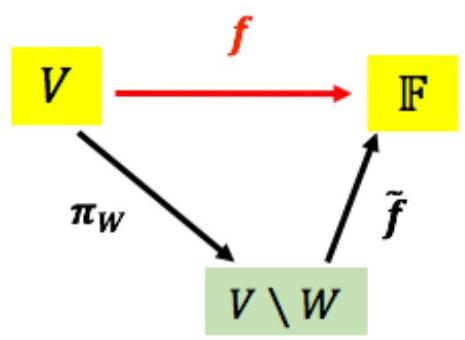
\includegraphics[max width=0.3\textwidth]{images/bo_d1h964v7aajc7382l5mg_71_705_475_465_340_0.jpg}
\end{center}
\hspace*{3em} 

i.e., \(\widetilde{f}\left( {\mathbf{v} + W}\right)  = f\left( \mathbf{v}\right)\).

\section*{5.4. Wednesday for MAT 3040}

There will be a quiz on next Monday.

Scope: From Week 1 up to (including) the definition of \({B}^{ * }\).

\section*{Reviewing.}

1. If \(V\) is finite dimensional, and \(B\) a basis of \(V\), then \({B}^{ * }\) is a basis of the dual space \({V}^{ * }\).

2. Define the Annihilator \(\operatorname{Ann}\left( S\right)  \leq  {V}^{ * }\) :

\[
\operatorname{Ann}\left( S\right)  = \left\{  {f \in  {V}^{ * } \mid  f\left( s\right)  = 0,\forall s \in  S}\right\}
\]

3. If \(V\) is finite dimensional, and \(W \leq  V\), then \(\operatorname{Ann}\left( W\right)\) fills the gap, i.e.,

\[
\dim \left( {\operatorname{Ann}\left( W\right) }\right)  = \dim \left( V\right)  - \dim \left( W\right)
\]

4. Define a map

\[
\Phi  : \operatorname{Ann}\left( W\right)  \rightarrow  {\left( V/W\right) }^{ * }
\]

\[
f \mapsto  \widetilde{f}
\]

where \(\widetilde{f}\) is defined such that the diagram (5.1) below commutes

\begin{center}
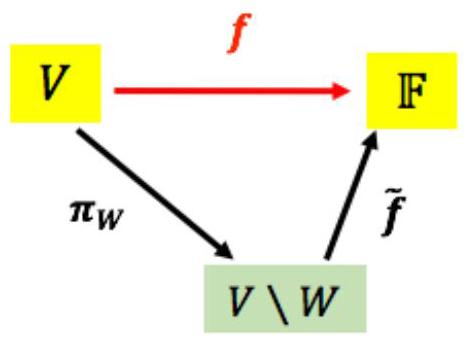
\includegraphics[max width=0.3\textwidth]{images/bo_d1h964v7aajc7382l5mg_72_558_1557_464_337_0.jpg}
\end{center}
\hspace*{3em} 

Figure 5.1: Construction of \(\widetilde{f}\)

Or equivalently, \(\widetilde{f} : V/W \rightarrow  \mathbb{F}\) is such that \(\widetilde{f}\left( {\mathbf{v} + W}\right)  = f\left( \mathbf{v}\right)\).

\section*{5.4.1. Adjoint Map}

The natural question is that whether \(\Phi\) is the isomorphism between \(\operatorname{Ann}\left( W\right)\) and \({\left( V/W\right) }^{ * }\) :

Proposition \({5.4}\;\Phi\) is a linear transformation, i.e.,

\[
\Phi \left( {{af} + {bg}}\right)  = a \cdot  \Phi \left( f\right)  + b \cdot  \Phi \left( g\right) .
\]

Proof. Itt suffices to show that

\[
\overline{{af} + {bg}} = a\bar{f} + b\bar{g}
\]

Therefore, we need to answer whether \(\Phi\) a bijective map. We will show this conjucture at the end of this lecture. The definition of \(\Phi\) is natural, i.e., we do not need to specify any basis to define this \(\Phi\). However, as studied in Monday, the constructed isomorphism \(V \rightarrow  {V}^{ * }\) with \({\bf v}_{i} \mapsto  {f}_{i}\) is not natural.

Definition 5.3 [Adjoint Map] Let \(T : V \rightarrow  W\) be a linear transformation. Define the adjoint of \(T\) by

\[
{T}^{ * } : \;{W}^{ * } \rightarrow  {V}^{ * }
\]

such that for any \(f \in  {W}^{ * }\),

\[
\left\lbrack  {{T}^{ * }\left( f\right) }\right\rbrack  \left( \mathbf{v}\right)  \mathrel{\text{ := }} f\left( {T\left( \mathbf{v}\right) }\right) ,\forall \mathbf{v} \in  V.
\]

1. In other words, \({T}^{ * }\left( f\right)  = f \circ  T\), i.e., a linear transformation from \(V\) to \(\mathbb{F}\), i.e., belongs to \({V}^{ * }\).

2. Moreover, the mapping \({T}^{ * }\) itself is a linear transformation: For \(f,g \in  {W}^{ * }\),

and \(\forall v \in  V\),

\[
\left\lbrack  {{T}^{ * }\left( {{af} + {bg}}\right) }\right\rbrack  \left( \mathbf{v}\right)  = \left( {{af} + {bg}}\right) \left\lbrack  {T\left( \mathbf{v}\right) }\right\rbrack
\]

\[
= {af}\left( {T\left( \mathbf{v}\right) }\right)  + {bg}\left( {T\left( \mathbf{v}\right) }\right)
\]

\[
= a\left\lbrack  {{T}^{ * }\left( f\right) }\right\rbrack  \left( \mathbf{v}\right)  + b\left\lbrack  {{T}^{ * }\left( g\right) }\right\rbrack  \left( \mathbf{v}\right)
\]

\[
= \left\lbrack  {a{T}^{ * }\left( f\right)  + b{T}^{ * }\left( g\right) }\right\rbrack  \left( \mathbf{v}\right)
\]

definition of \({V}^{ * }\) as a vector space

Proposition 5.5 Let \(T : V \rightarrow  W\) be a linear transformation.

1. If \(T\) is injective, then \({T}^{ * }\) is surjective.

2. If \(T\) is surjetive, then \({T}^{ * }\) is injective.

This statement is quite intuitive, since \({T}^{ * }\) reverses the dual of output into the dual of input:

\[
T : V \rightarrow  W
\]

\[
{T}^{ * } : {W}^{ * } \rightarrow  {V}^{ * }
\]

Proof. We only give a proof of (2), i.e., suffices to show \(\ker \left( T\right)  = \{ \mathbf{0}\}\).

Consider any \(g \in  {W}^{ * }\) such that \({T}^{ * }\left( g\right)  = {\mathbf{0}}_{{V}^{ * }}\). It follows that

\[
\left\lbrack  {{T}^{ * }\left( g\right) }\right\rbrack  \left( \mathbf{v}\right)  = {\mathbf{0}}_{{V}^{ * }}\left( \mathbf{v}\right) ,\;\forall \mathbf{v} \in  V. \Leftrightarrow  g\left( {T\left( \mathbf{v}\right) }\right)  = \mathbf{0},\;\forall \mathbf{v} \in  V. \tag{5.4}
\]

To show \(g = {\mathbf{0}}_{{W}^{ * }}\), it suffices to show \(g\left( \mathbf{w}\right)  = \mathbf{0}\) for all \(\mathbf{w} \in  W\). For all \(\mathbf{w} \in  W\), by the surjectivity of \(T\), there exists \({\bf v}^{\prime } \in  V\) such that

\[
\mathbf{w} = T\left( {\bf v}^{\prime }\right) .
\]

By substituting \(\mathbf{w}\) with \(T\left( {\bf v}^{\prime }\right)\) and (5.4), we imply

\[
g\left( \mathbf{w}\right)  = g\left( {T\left( {\bf v}^{\prime }\right) }\right)  = \mathbf{0}.
\]

The proof is complete.

Proposition 5.6 Let \(T : V \rightarrow  W\) be a linear transformation, and \(\mathcal{A} = \left\{  {{\bf v}_1,\ldots ,{\bf v}_n}\right\}  ,\mathcal{B} =\)  \(\left\{  {{\bf w}_1,\ldots ,{\bf w}_{m}}\right\}\) be the bases of \(V\) and \(W\), respectively. Let \({\mathcal{A}}^{ * } = \left\{  {{f}_1,\ldots ,{f}_n}\right\}  ,{\mathcal{B}}^{ * } = \left\{  {{g}_1,\ldots ,{g}_{m}}\right\}\)

be bases of dual spaces \({V}^{ * }\) and \({W}^{ * }\), respectively. Then \({T}^{ * } : {W}^{ * } \rightarrow  {V}^{ * }\) admits a matrix representation

\[
{\left( {T}^{ * }\right) }_{{\mathcal{A}}^{ * }{\mathcal{B}}^{ * }} = \operatorname{transpose}\left( {\left( T\right) }_{\mathcal{B}\mathcal{A}}\right)
\]

where \({\left( {T}^{ * }\right) }_{{\mathcal{A}}^{ * }{\mathcal{B}}^{ * }} \in  {\mathbb{F}}^{n \times  m}\) and \({\left( T\right) }_{\mathcal{B}\mathcal{A}} \in  {\mathbb{F}}^{m \times  n}\)

Proof. Let \({\left( T\right) }_{\mathcal{{BA}}} = \left( \alpha_{ij}\right)\) and \({\left( {T}^{ * }\right) }_{{\mathcal{A}}^{ * }{\mathcal{B}}^{ * }} = \left( \beta_{ij}\right)\). By definition of matrix representation,

\[
T\left( {\bf v}_{j}\right)  = \mathop{\sum }\limits_{{i = 1}}^{m}\alpha_{ij}{\bf w}_{i},\;{T}^{ * }\left( {g}_{i}\right)  = \mathop{\sum }\limits_{{k = 1}}^n\beta_{ki}{f}_{k} \in  {V}^{ * }
\]

As a result,

\[
\left\lbrack  {{T}^{ * }\left( {g}_{i}\right) }\right\rbrack  \left( {\bf v}_{j}\right)  = {g}_{i}\left( {T\left( {\bf v}_{j}\right) }\right)
\]

\[
= {g}_{i}\left( {\mathop{\sum }\limits_{{\ell  = 1}}^{m}\alpha_{\ell j}{\bf w}_{\ell }}\right)
\]

\[
= \mathop{\sum }\limits_{{\ell  = 1}}^{m}\alpha_{\ell j}{g}_{i}\left( {\bf w}_{\ell }\right)
\]

\[
= \alpha_{ij}
\]

and

\[
\left\lbrack  {{T}^{ * }\left( {g}_{i}\right) }\right\rbrack  \left( {\bf v}_{j}\right)  = \left( {\mathop{\sum }\limits_{{k = 1}}^n\beta_{ki}{f}_{k}}\right) \left( {\bf v}_{j}\right)
\]

\[
= \mathop{\sum }\limits_{{k = 1}}^n\beta_{ki}{f}_{k}\left( {\bf v}_{j}\right)
\]

\[
= \beta_{ji}
\]

Therefore, \(\beta_{ji} = \alpha_{ij}\). The proof is complete.

\section*{5.4.2. Relationship between Annihilator and dual}

of quotient spaces


\begin{itemize}
\item Example 5.5 Consider the canonical projection mapping \({\pi }_{W} : V \rightarrow  V/W\) with its adjoint
\end{itemize}

mapping:

\[
{\left( {\pi }_{W}\right) }^{ * } : {\left( V/W\right) }^{ * } \rightarrow  {V}^{ * }
\]

The understanding of \({\left( {\pi }_{W}\right) }^{ * }\) is as follows:

\hspace*{2em} 1. Take \(h \in  {\left( V/W\right) }^{ * }\) and study \({\left( {\pi }_{W}\right) }^{ * }\left( h\right)  \in  {V}^{ * }\)

\hspace*{2em} 2. Take \(v \in  V\) and understand

\[
\left\lbrack  {{\left( {\pi }_{W}\right) }^{ * }\left( h\right) }\right\rbrack  \left( \mathbf{v}\right)  = h\left( {{\pi }_{W}\left( \mathbf{v}\right) }\right)  = h\left( {\mathbf{v} + W}\right)
\]

\hspace*{1em} (a) In particular, for all \(w \in  W \leq  V\), we have

\[
\left\lbrack  {{\left( {\pi }_{W}\right) }^{ * }\left( h\right) }\right\rbrack  \left( \mathbf{w}\right)  = h\left( {\mathbf{w} + W}\right)  = h\left( {\mathbf{0}}_{V/W}\right)  = {\mathbf{0}}_{\mathbb{F}}
\]

\hspace*{3em} Therefore,

\[
{\left( {\pi }_{W}\right) }^{ * }\left( h\right)  \in  \operatorname{Ann}\left( W\right) \text{ . }
\]

\hspace*{3em} i.e., \({\left( {\pi }_{W}\right) }^{ * }\) is a mapping from \({\left( V/W\right) }^{ * }\) to \(\operatorname{Ann}\left( W\right)\).

\hspace*{1em} (b) By proposition (5.5), \({\pi }_{W}\) is surjective implies \({\left( {\pi }_{W}\right) }^{ * }\) is injective.

Combining (a) and (b), it's clear that (i.e., left as homework problem)

\[
\Phi  \circ  {\pi }_{W}^{ * } = {\operatorname{id}}_{{\left( V/W\right) }^{ * }}\text{ and }{\pi }_{W}^{ * } \circ  \Phi  = {\operatorname{id}}_{\operatorname{Ann}\left( W\right) }
\]

This relationship implies \(\Phi\) is an isomorphism.

\HRule

\section*{Chapter 6}

\section*{Week6}

\section*{6.1. Monday for MAT 3040}

\section*{6.1.1. Polynomials}

We recall some useful properties of polynomial before studying eigenvalues/eigenvectors.

Definition 6.1 [Polynomial]

1. A polynomial over \(\mathbb{F}\) has the form

\[
p\left( z\right)  = {a}_{m}{z}^{m} + \cdots  + {a}_1z + {a}_{0},\;\left( {{a}_{m} \neq  0}\right) .
\]

Here \({a}_{m}{z}^{m}\) is called the leading term of \(p\left( z\right) ;m\) is called the degree; \({a}_{m}\) is called the leading coefficient; \({a}_{m},\cdots ,{a}_{0}\) are called the coefficients of this polynomial.

2. A polynomial over \(\mathbb{F}\) is monic if its leading coefficient is \(1_{\mathbb{F}}\).

3. A polynomial \(p\left( z\right)  \in  \mathbb{F}\left\lbrack  z\right\rbrack\) is irreducible if for any \(a\left( z\right) ,b\left( z\right)  \in  \mathbb{F}\left\lbrack  z\right\rbrack\),

\[
p\left( z\right)  = a\left( z\right) b\left( z\right)  \Rightarrow  \text{ either }a\left( z\right) \text{ or }b\left( z\right) \text{ is a constant polynomial. }
\]

Otherwise \(p\left( z\right)\) is reducible.

\begin{itemize}
\item Example 6.1 For example, the polynomial \(p\left( x\right)  = {x}^2 + 1\) is irreducible over \(\mathbb{R}\) ; but \(p\left( x\right)  = \left( {x - i}\right) \left( {x + i}\right)\) is reducible over \(\mathbb{C}\).
\end{itemize}

Theorem 6.1 - Division Theorem. For all \(p,q \in  \mathbb{F}\left\lbrack  z\right\rbrack\) such that \(p \neq  0\), there exists unique \(s,r \in  \mathbb{F}\left\lbrack  x\right\rbrack\) satisfying \(\deg \left( r\right)  < \deg \left( f\right)\), such that

\[
p\left( z\right)  = s\left( z\right)  \cdot  q\left( z\right)  + r\left( z\right) .
\]

Here \(r\left( z\right)\) is called the remainder.

\begin{itemize}
\item Example 6.2 Given \(p\left( x\right)  = {x}^{4} + 1\) and \(q\left( x\right)  = {x}^2 + 1\), the junior school knowledge tells us that uniquely
\end{itemize}

\[
{x}^{4} + 1 = \left( {{x}^2 - 1}\right) \left( {{x}^2 + 1}\right)  + 2.
\]

Theorem 6.2 - Root Theorem. For \(p\left( x\right)  \in  \mathbb{F}\left\lbrack  x\right\rbrack\), and \(\lambda  \in  \mathbb{F},x - \lambda\) divides \(p\) if and only if \(p\left( \lambda \right)  = 0\).

Proof. 1. If \(\left( {x - \lambda }\right)\) divides \(p\), then \(p = \left( {x - \lambda }\right) q\) for some \(q \in  \mathbb{F}\left\lbrack  x\right\rbrack\). Thus clearly \(p\left( \lambda \right)  = 0\).

2. For the other direction, suppose that \(p\left( \lambda \right)  = 0\). By division theorem, there exists \(s,r \in  \mathbb{F}\left\lbrack  x\right\rbrack\) such that

\[
p = \left( {x - \lambda }\right) s + r\;\text{ with }\deg \left( r\right)  < \deg \left( {x - \lambda }\right)  = 1. \tag{6.1}
\]

Therefore, the polynomial \(r\) must be constant.

Substituting \(\lambda\) into \(x\) both sides in (6.1), we have

\[
0 = p\left( \lambda \right)  = 0 \cdot  s + r \Rightarrow  r = 0.
\]

Therefore, \(p = \left( {x - \lambda }\right)  \cdot  s\), i.e., \(\left( {x - \lambda }\right)\) divides \(p\).

\section*{6.4. Wednesday for MAT 3040}

Reviewing: Root Theorem: \(p\left( \lambda \right)  = 0\) iff \(\left( {x - \lambda }\right)\) divdes \(p\left( x\right)\).

Corollary 6.2 A polynomial with degree \(n\) has at most \(n\) roots counting multiplicity.

For example, the polynomial \({\left( x - 3\right) }^2\) has one root \(x = 3\) with multiplicity 2 . When counting multiplicity, we say the polynomial \({\left( x - 3\right) }^2\) has two roots.

Definition 6.5 [Algebraically Closed] A field \(\mathbb{F}\) is called algebraically closed if every non-constant polynomial \(p\left( x\right)  \in  \mathbb{F}\left\lbrack  x\right\rbrack\) has a root \(\lambda  \in  \mathbb{F}\).

Theorem 6.5 - Fundamental Theroem of Algebra. The set of complex numbers \(\mathbb{C}\) is algebraically closed.

Proof. One way is by complex analysis; Another way is by the topology on \(\mathbb{C} \smallsetminus  \{ 0\}\).

By induction, we can show that every polynomial with degree \(n\) on algebraically closed field \(\mathbb{F}\) has exactly \(n\) roots, counting multiplicity. Therefore, for any \(p\left( x\right)\) on algebraically closed field \(\mathbb{F}\),

\[
p\left( x\right)  = c\left( {x - {\lambda }_1}\right) \cdots \left( {x - {\lambda }_n}\right)  \tag{6.3}
\]

for \(c,{\lambda }_1,\ldots ,{\lambda }_n \in  \mathbb{F}\).

The polynomials on general field \(\mathbb{F}\) may not necessarily be factorized as in (6.3), but still admit unique factorization property:

Theorem 6.6 - Unique Factorization. Every \(f\left( x\right)  = {a}_n{x}^n + \cdots  + {a}_{0}\) in \(\mathbb{F}\left\lbrack  x\right\rbrack\) can be factorized as

\[
f\left( x\right)  = {a}_n{\left\lbrack  {p}_1\left( x\right) \right\rbrack  }^{{e}_1}\cdots {\left\lbrack  {p}_{k}\left( x\right) \right\rbrack  }^{{e}_{k}}
\]

where \({p}_{i}\) ’s are monic, irreducible, distinct. Furthermore, this expression is unique up to the permutation of factors. Definition 6.6 [Factor] If \(p\left( x\right)  = q\left( x\right) s\left( x\right)\) with \(p,q,s \in  \mathbb{F}\left\lbrack  x\right\rbrack\), then we say

\begin{itemize}
\item \(p\left( x\right)\) is divisible by \(s\left( x\right)\) ;
\end{itemize}

\begin{itemize}
\item \(s\left( x\right)\) is a factor of \(p\left( x\right)\) ;
\end{itemize}

\begin{itemize}
\item \(s\left( x\right)  \mid  p\left( x\right)\)
\end{itemize}

\begin{itemize}
\item \(s\left( x\right)\) divides \(p\left( x\right)\)
\end{itemize}

\begin{itemize}
\item \(p\left( x\right)\) is multiple of \(s\left( x\right)\)
\end{itemize}

\section*{Definition 6.7 [Common Factor]}

1. The polynomial \(g\left( x\right)\) is said to be a common factor of \({f}_1,\ldots ,{f}_{k} \in  \mathbb{F}\left\lbrack  x\right\rbrack\) if

\[
g \mid  {f}_{i},i = 1,\ldots ,k
\]

2. The polynomial \(g\left( x\right)\) is said to be a greatest common divisor of \({f}_1,\ldots ,{f}_{k}\) if

\begin{itemize}
\item \(g\) is monic.
\end{itemize}

\begin{itemize}
\item \(g\) is common factor of \({f}_1,\ldots ,{f}_{k}\)
\end{itemize}

\begin{itemize}
\item \(g\) is of largest possible (maximal) degree.
\end{itemize}

\begin{itemize}
\item \(\gcd \left( {{f}_1,\ldots ,{f}_{k}}\right)  = \gcd \left( {\gcd \left( {{f}_1,{f}_2}\right) ,{f}_{3},\ldots ,{f}_{k}}\right)  = \gcd \left( {\gcd \left( {{f}_1,{f}_2,{f}_{3}}\right) ,\ldots ,{f}_{k}}\right)\)
\end{itemize}

\begin{itemize}
\item \(\gcd \left( {{f}_1,\ldots ,{f}_{k}}\right)\) is unique.
\end{itemize}

\begin{itemize}
\item If \(\gcd \left( {{f}_1,\ldots ,{f}_{k}}\right)  = 1\), we say \({f}_1,\ldots ,{f}_{k}\) is relatively prime
\end{itemize}

\begin{itemize}
\item Polynomials \({f}_1,\ldots ,{f}_{k}\) are relatively prime does not necessarily mean \(\gcd \left( {{f}_{i},{f}_{j}}\right)  = 1\) for any \(i \neq  j\).
\end{itemize}

Counter-example: Let \({a}_1,\ldots ,{a}_n\) distinct irreducible polynomials, and

\[
{f}_{i}\left( x\right)  = {a}_1\left( x\right) \cdots {\widehat{a}}_{i}\left( x\right) \cdots {a}_n\left( x\right)  \mathrel{\text{ := }} {a}_1\cdots {a}_{i - 1}{a}_{i + 1}\cdots {a}_n,
\]

then \(\gcd \left( {{f}_1,\ldots ,{f}_n}\right)  = 1\), but \(\gcd \left( {{f}_{i},{f}_{j}}\right)  = {a}_1\cdots {\widehat{a}}_{i}\cdots {\widehat{a}}_{j}\cdots {a}_n\), which does not necessarily equal to 1 .

\begin{itemize}
\item Example 6.6 The \(\gcd \left( {{f}_1,{f}_2}\right)\) is easy to compute for factorized polynomials. For example, let \({f}_1\left( x\right)  = {\left( {x}^2 + x + 1\right) }^{3}{\left( x - 3\right) }^2{x}^{4}\) and \({f}_2\left( x\right)  = \left( {{x}^2 + 1}\right) {\left( x - 3\right) }^{4}{x}^2\) in \(\mathbb{R}\left\lbrack  x\right\rbrack\), then
\end{itemize}

\[
\gcd \left( {{f}_1,{f}_2}\right)  = {\left( x - 3\right) }^2{x}^2
\]

The question is how to find \(\gcd \left( {{f}_1,{f}_2}\right)\) for given un-factorized polynomials?

Theorem 6.7 - Bezout. Let \(g = \gcd \left( {{f}_1,{f}_2}\right)\), then there exists \({r}_1,{r}_2 \in  \mathbb{F}\left\lbrack  x\right\rbrack\) such that

\[
g\left( x\right)  = {r}_1\left( x\right) {f}_1\left( x\right)  + {r}_2\left( x\right) {f}_2\left( x\right)
\]

More generally, \(g = \gcd \left( {{f}_1,\ldots ,{f}_{k}}\right)\) implies there exists \({r}_1,\ldots ,{r}_{k}\) such that

\[
g = {r}_1{f}_1 + \cdots  + {r}_{k}{f}_{k}
\]

The derivation of \({r}_{i}\) ’s is by applying Euclidean algorithm. For example, given \({x}^{3} +\)  \({6x} + 7\) and \({x}^2 + {3x} + 2\), we imply

\[
{x}^{3} + {6x} + 7 - \left( {x - 3}\right) \left( {{x}^2 + {3x} + 2}\right)  = {13x} + {13}
\]

and

\[
{x}^2 + {3x} + 2 - \frac{x + 2}{13}\left( {{13x} + {13}}\right)  = 0
\]

Therefore, \(\gcd \left( {{x}^{3} + {6x} + 7,{x}^2 + {3x} + 2}\right)  = \gcd \left( {{x}^2 + {3x} + 2,{13x} + {13}}\right)  = x + 2\).

\section*{6.4.1. Eigenvalues \& Eigenvectors}

Definition 6.8 [Eigenvalues] Let \(T : V \rightarrow  V\) be a linear operator.

1. We say \(v \in  V \smallsetminus  \{ \mathbf{0}\}\) is an eigenvector of \(T\) with eigenvalue \(\lambda\) if \(T\left( v\right)  = {\lambda v}\) ;

2. Or equivalently, \(v \in  \ker \left( {T - {\lambda I}}\right)\), the \(\lambda\) -eigenspace of \(T\). Here the mapping \(I : V \rightarrow  V\) denotes identity map, i.e., \(I\left( \mathbf{v}\right)  = \mathbf{v},\forall \mathbf{v} \in  V\).

Definition 6.9 A vector \(v \in  V \smallsetminus  \{ \mathbf{0}\}\) is a generalized eigenvector of \(T\) with generalized eigenvalue \(\lambda\) if \(v \in  \ker \left( {\left( T - \lambda I\right) }^{k}\right)\) for some \(k \in  {\mathbb{N}}^{ + }\).

Note that an eigenvector is a generalized eigenvector of \(T\) ; while the converse does not necessarily hold.

\begin{itemize}
\item Example 6.7 Consider the linear transformation \(A : {\mathbb{R}}^2 \rightarrow  {\mathbb{R}}^2\) with
\end{itemize}

\[
A : \;{\mathbb{R}}^2 \rightarrow  {\mathbb{R}}^2
\]

\[
\text{ with }\mathbf{x} \rightarrow  \mathbf{{Ax}}
\]

\[
\text{ where }A = \left( \begin{array}{ll} 1 & 1 \\  0 & 1 \end{array}\right)
\]

1. Note that \({\left\lbrack  1,0\right\rbrack  }^{\mathrm{T}}\) is an eigenvector with eigenvalue 1, since

\[
A\left( \begin{array}{l} 1 \\  0 \end{array}\right)  = \left( \begin{array}{l} 1 \\  0 \end{array}\right)
\]

2. However, \({\left\lbrack  0,1\right\rbrack  }^{\mathrm{T}}\) is not an eigenvector, since

\[
A\left( \begin{array}{l} 0 \\  1 \end{array}\right)  = \left( \begin{array}{l} 1 \\  0 \end{array}\right) .
\]

Note that

\[
{\left( A - I\right) }^2 = \left( \begin{array}{ll} 0 & 1 \\  0 & 0 \end{array}\right) ,\;{\left( A - I\right) }^{3} = \left( \begin{array}{ll} 0 & 0 \\  0 & 0 \end{array}\right)
\]

and therefore

\[
\left( \begin{array}{l} 0 \\  1 \end{array}\right)  \in  \ker {\left( A - I\right) }^2
\]

i.e., a generalized eigenvector with generalized eigenvalue 1 .

\begin{itemize}
\item Example 6.8 Consider \(V = {C}^{\infty }\left( \mathbb{R}\right)\), which is a set of all infinitely differentiable functions.
\end{itemize}

Define the linear operator \(T : V \rightarrow  V\) as \(T\left( f\right)  = {f}^{\prime \prime }\). Then the(-1)-eigenspace of \(T\) has \(f \in  V\) satisfying

\[
{f}^{\prime \prime } =  - f
\]

From ODE course, we imply \(\{ \sin x,\cos x\}\) forms a basis of (-1)-eigenspace.

Assumption. From now on, we assume \(V\) has finite dimension by default.

Definition 6.10 [Determinant] Let \(T : V \rightarrow  V\) be a linear operator. The determinant of \(T\) is given by

\[
\det \left( T\right)  = \det \left( {\left( T\right) }_{\mathcal{A},\mathcal{A}}\right)
\]

where \(\mathcal{A}\) is some basis of \(V\).

Assume we have complete knowledge about \(\det \left( M\right)\) for matrices for now. The determinant is well-defined, i.e., independent of the choice of basis \(\mathcal{A}\). For another basis \(\mathcal{B}\), we imply

\(\det \left( {T}_{\mathcal{B},\mathcal{B}}\right)  = \det \left( {{C}_{\mathcal{B},\mathcal{A}}{T}_{\mathcal{A},\mathcal{A}}{C}_{\mathcal{A},\mathcal{B}}}\right)  = \det \left( {C}_{\mathcal{B},\mathcal{A}}\right) \det \left( {T}_{\mathcal{A},\mathcal{A}}\right) \det \left( {C}_{\mathcal{A},\mathcal{B}}\right)  = \det \left( {T}_{\mathcal{A},\mathcal{A}}\right)\)

Definition 6.11 [characteristic polynomial] The characteristic polynomial \({X}_{T}\left( x\right)\) of \(T : V \rightarrow  V\) is defined as

\[
{\mathcal{X}}_{T}\left( x\right)  = \det \left( {{\left( T\right) }_{\mathcal{A},\mathcal{A}} - {xI}}\right)
\]

for any basis \(\mathcal{A}\)

In the next few lectures, we will study

\begin{itemize}
\item Cayley-Hamilton Theorem
\end{itemize}

\begin{itemize}
\item Jordan Canonical Form
\end{itemize}

These theorems can be stated using matrices, and they both hold up to change of basis. We have a unified statement of these theorem using vecotor space rather than \({\mathbb{R}}^n\).


\section*{Chapter 7 Week7}

\section*{7.1. Monday for MAT 3040}

Reviewing. Define the characteristic polynomial for an linear operator \(T\) :

\[
{\mathcal{X}}_{T}\left( x\right)  = \det \left( {{\left( T\right) }_{\mathcal{A},\mathcal{A}} - x\mathbf{I}}\right)
\]

We will use the notation " \(I/{I}^{\prime \prime }\) in two different occasions:

1. I denotes the identity transformation from \(V\) to \(V\) with \(I\left( \mathbf{v}\right)  = \mathbf{v},\forall \mathbf{v} \in  V\)

2. \(\mathbf{I}\) denotes the identity matrix \({\left( I\right) }_{\mathcal{A},\mathcal{A}}\), defined based on any basis \(\mathcal{A}\).

\section*{7.1.1. Minimal Polynomial}

Definition 7.1 [Linear Operator Induced From Polynomial] Let \(f\left( x\right)  \mathrel{\text{ := }} {a}_{m}{x}^{m} + \cdots  + {a}_{0}\) be a polynomial in \(\mathbb{F}\left\lbrack  x\right\rbrack\), and \(T : V \rightarrow  V\) be a linear operator. Then the mapping

\[
f\left( T\right)  = {a}_{m}{T}^{m} + \cdots  + {a}_1T + {a}_{0}I : \;V \rightarrow  V,
\]

is called a linear operator induced from the polynomial \(f\left( x\right)\).

1. The composition of linear operators is not abelian, e.g., in general \(S \circ  T =\)  \(T \circ  S\) does not hold. The reason follows similarly from the fact that square-matrix multiplication is not abelian in general.

2. However, we always have \(f\left( T\right) T = {Tf}\left( T\right)\), where \(f\left( T\right)\) is a linear operator induced from the polynomial \(f\left( x\right)\) :

Proof. We can show that \({T}^nT = T{T}^n,\forall n\) by induction. Suppose that \(f\left( x\right)  =\)  \(\mathop{\sum }\limits_{i}{a}_{i}{x}^{i}\), which follows that

\[
f\left( T\right) T = \mathop{\sum }\limits_{i}{a}_{i}{T}^{i}T = \mathop{\sum }\limits_{i}{a}_{i}T{T}^{i} = T\mathop{\sum }\limits_{i}{a}_{i}{T}^{i} = {Tf}\left( T\right) .
\]

3. We can generalize the statement in (2) into the fact that the composition of linear operators induced from polynomials is abelian, i.e.,

\[
f\left( T\right) g\left( T\right)  = g\left( T\right) f\left( T\right)
\]

for any polynomials \(f\left( x\right) ,g\left( x\right)\). Definition 7.2 [Minimal Polynomial] Let \(T : V \rightarrow  V\) be a linear operator. The minimal polynomial \({m}_{T}\left( x\right)\) is a nonzero monic polynomial of least (minimal) degree such that

\[
{m}_{T}\left( T\right)  = {\mathbf{0}}_{V \rightarrow  V}.
\]

where \({\mathbf{0}}_{V \rightarrow  V}\) denotes the zero vector in \(\operatorname{Hom}\left( {V,V}\right)\).

cample 7.1 1. Let \(A = \left( \begin{array}{ll} 1 & 0 \\  0 & 1 \end{array}\right)\), then \(A\) defines a linear operator:

\[
A : \;{\mathbb{F}}^2 \rightarrow  {\mathbb{F}}^2
\]

\[
\text{ with }\mathbf{x} \mapsto  \mathbf{{Ax}}
\]

Here \({\mathcal{X}}_{A}\left( x\right)  = {\left( x - 1\right) }^2\) and \(A - \mathbf{I} = \mathbf{0}\), which gives \({m}_{A}\left( x\right)  = x - 1\).

2. Let \(B = \left( \begin{array}{ll} 1 & 1 \\  0 & 1 \end{array}\right)\), which implies

\[
{\mathcal{X}}_{B}\left( x\right)  = {\left( x - 1\right) }^2,
\]

The question is that can we get the minimal polynomial with degree 1 ?

The answer is no, since \(B - k\mathbf{I} = \left( \begin{matrix} 1 - k & 1 \\  0 & 1 - k \end{matrix}\right)  \neq  \mathbf{0}\).

In fact, \({m}_{B}\left( x\right)  = {\left( x - 1\right) }^2\), since

\[
{\left( B - \mathbf{I}\right) }^2 = {\left( \begin{array}{ll} 0 & 1 \\  0 & 0 \end{array}\right) }^2 = \left( \begin{array}{ll} 0 & 0 \\  0 & 0 \end{array}\right) .
\]

Two questions naturally arises:

1. Does \({m}_{T}\left( x\right)\) exist? If exists, is it unique?

2. What’s the relationship between \({m}_{T}\left( x\right)\) and \({\mathcal{X}}_{T}\left( x\right)\) ?

Regarding to the first question, the minimal polynomial \({m}_{T}\left( x\right)\) may not exist, if \(V\) has infinite dimension:

\begin{itemize}
\item Example 7.2 Consider \(V = \mathbb{R}\left\lbrack  x\right\rbrack\) and the mapping
\end{itemize}

\[
T : \;V \rightarrow  V
\]

\[
p\left( x\right)  \mapsto  {\int }_{0}^{x}p\left( t\right) \mathrm{d}t
\]

In particular, \(T\left( {x}^n\right)  = \frac1{n + 1}{x}^{n + 1}\). Suppose \({m}_{T}\left( x\right)\) is with degree \(n\), i.e.,

\[
{m}_{T}\left( x\right)  = {x}^n + \cdots  + {a}_1x + {a}_{0},
\]

then

\[
{m}_{T}\left( T\right)  = {T}^n + \cdots  + {a}_{0}I\text{ is a zero linear transformation }
\]

It follows that

\[
\left\lbrack  {{m}_{T}\left( T\right) }\right\rbrack  \left( x\right)  = \frac1{n!}{x}^n + {a}_{n - 1}\frac1{\left( {n - 1}\right) !}{x}^{n - 1} + \cdots  + {a}_1x + {a}_{0} = {0}_{\mathbb{F}},
\]

which is a contradiction since the coefficients of \({x}^{k}\) is nonzero on LHS for \(k = 1,\ldots ,n\), but zero on the RHS.

Proposition 7.1 The minimal polynomial \({m}_{T}\left( x\right)\) always exists for \(\dim \left( V\right)  = n < \infty\).

Proof. It’s clear that \(\left\{  {I,T,\ldots ,{T}^n,{T}^{n + 1},\cdots ,{T}^{n^2}}\right\}   \subseteq  \operatorname{Hom}\left( {V,V}\right)\). Since \(\dim \left( {\operatorname{Hom}\left( {V,V}\right) }\right)  = n^2\), we imply \(\left\{  {I,T,\ldots ,{T}^n,{T}^{n + 1},\cdots ,{T}^{n^2}}\right\}\) is linearly dependent, i.e., there exists \({a}_{i}\) ’s that are not all zero such that

\[
{a}_{0}I + {a}_1T + \cdots  + {a}_{n^2}{T}^{n^2} = 0
\]

i.e., there is a polynomial \(g\left( x\right)\) of degree less than \(n^2\) such that \(g\left( T\right)  = 0\).

The proof is complete.

Proposition 7.2 The minimal polynomial \({m}_{T}\left( x\right)\), if exists, then it exists uniquely.

Proof. Suppose \({f}_1,{f}_2\) are two distinct minimal polynomials with \(\deg \left( {f}_1\right)  = \deg \left( {f}_2\right)\). It follows that

\begin{itemize}
\item \(\deg \left( {{f}_1 - {f}_2}\right)  < \deg \left( {f}_1\right)\).
\end{itemize}

\begin{itemize}
\item \({f}_1 - {f}_2 \neq  0\)
\end{itemize}

\begin{itemize}
\item \(\left( {{f}_1 - {f}_2}\right) \left( T\right)  = {f}_1\left( T\right)  - {f}_2\left( T\right)  = {0}_{V \rightarrow  V}\)
\end{itemize}

By scaling \({f}_1 - {f}_2\), there is a monic polynomial \(g\) with lower degree satisfying \(g\left( T\right)  = 0\), which contradicts the definition for minimal polynomial.

Proposition 7.3 Suppose \(f\left( x\right)  \in  \mathbb{F}\left\lbrack  x\right\rbrack\) satisfying \(f\left( T\right)  = 0\), then

\[
{m}_{T}\left( x\right)  \mid  f\left( x\right) \text{ . }
\]

Proof. It’s clear that \(\deg \left( f\right)  \geq  \deg \left( {m}_{T}\right)\). The division algorithm gives

\[
f\left( x\right)  = q\left( x\right) {m}_{T}\left( x\right)  + r\left( x\right) .
\]

Therefore, for any \(\mathbf{v} \in  V\)

\[
\left\lbrack  {r\left( T\right) }\right\rbrack  \left( \mathbf{v}\right)  = \left\lbrack  {f\left( T\right) }\right\rbrack  \left( \mathbf{v}\right)  - \left\lbrack  {q\left( T\right) {m}_{T}\left( T\right) }\right\rbrack  \left( \mathbf{v}\right)  = {\mathbf{0}}_{V} - q\left( T\right) {\mathbf{0}}_{V} = {\mathbf{0}}_{V} - {\mathbf{0}}_{V} = {\mathbf{0}}_{V}
\]

Therefore, \(r\left( T\right)  = {\mathbf{0}}_{V \rightarrow  V}\). By definition of minimal polynomial, we imply \(r\left( x\right)  \equiv  0\).

Proposition 7.4 If \(A,B \in  {\mathbb{F}}^{n \times  n}\) are similar to each other, then \({m}_{A}\left( x\right)  = {m}_{B}\left( x\right)\).

Proof. Suppose that \(B = {\mathbf{P}}^{-1}\mathbf{{AP}}\), and that

\[
{m}_{A}\left( x\right)  = {x}^{k} + \cdots  + {a}_1x + {a}_{0},\;{m}_{B}\left( x\right)  = {x}^{\ell } + \cdots  + {b}_{0}.
\]

It follows that

\[
{m}_{A}\left( B\right)  = {B}^{k} + \cdots  + {a}_{0}I
\]

\[
= {\mathbf{P}}^{-1}{A}^{k}\mathbf{P} + \cdots  + {a}_{0}{\mathbf{P}}^{-1}\mathbf{P}
\]

\[
= {\mathbf{P}}^{-1}\left( {{A}^{k} + \cdots  + {a}_{0}\mathbf{I}}\right) \mathbf{P}
\]

\[
= {\mathbf{P}}^{-1}\left( {{m}_{A}\left( A\right) }\right) \mathbf{P}
\]

Therefore, \({m}_{A}\left( B\right)  = \mathbf{0}\) since \({m}_{A}\left( A\right)  = \mathbf{0}\). By proposition (7.3), we imply \({m}_{B}\left( x\right)  \mid  {m}_{A}\left( x\right)\). Similarly, \({m}_{A}\left( x\right)  \mid  {m}_{B}\left( x\right)\). Since \({m}_{A}\left( x\right)\) and \({m}_{B}\left( x\right)\) are monic, we imply \({m}_{A}\left( x\right)  = {m}_{B}\left( x\right)\).

R Proposition (7.4) claims that the minimal polynomial is similarity-invariant; actually, the characteristic polynomial is similarity-invariant as well.

Assumption. We will asssume \(V\) has finite dimension from now on. Now we study the vanishing of a single vector \(\mathbf{v} \in  V\).

Notation. The \({m}_{T}\left( x\right)\) is a nonzero monic poylnomial of least degree such that

\[
{m}_{T}\left( T\right)  = {\mathbf{0}}_{V \rightarrow  V}\text{ . }
\]

\section*{7.1.2. Minimal Polynomial of a vector}

Definition 7.3 [Minimal Polynomial of a vector] Similar to the minimal polynomial, we define the minimal polynomial of a vector \(v\) relative to \(T\), say \({m}_{T,v}\left( x\right)\), as the monic polynomial of least degree such that

\[
{m}_{T,v}\left( T\right) \left( v\right)  = 0
\]

The existence of minimal polynomial of a vector is due to the existence of minimal polynomial; the uniqueness follows similarly as in proposition (7.2).

Proposition 7.5 Let \(T : V \rightarrow  V\) be a linear operator and \(v \in  V\). The degree of the minimal polynomial of a vector is upper bounded by:

\[
\deg \left( {{m}_{T,v}\left( x\right) }\right)  \leq  \dim \left( V\right) \text{ . }
\]

Proof. It’s clear that \(\left\{  {\mathbf{v},T\mathbf{v},\ldots ,{T}^n\mathbf{v}}\right\}   \subseteq  V\) and the proof follows similarly as in proposition (7.1).

Similar to the division property in proposition (7.3), we have the division proprty for minimal polynomial of a vector:

Proposition 7.6 Suppose \(f\left( x\right)  \in  \mathbb{F}\left\lbrack  x\right\rbrack\) satisfying \(f\left( T\right) \left( v\right)  = {\mathbf{0}}_{V}\), then

\[
{m}_{T,v}\left( x\right)  \mid  f\left( x\right) \text{ . }
\]

In particular, \({m}_{T,v} \mid  {m}_{T}\left( x\right)\).

Proof. The proof follows similarly as in proposition (7.3).

Proposition 7.7 Suppose that \({m}_{T,v}\left( x\right)  = {f}_1\left( x\right) {f}_2\left( x\right)\), where \({f}_1,{f}_2\) are both monic. Let \(\mathbf{w} = {f}_1\left( T\right) \mathbf{v}\), then

\[
{m}_{T,\mathbf{w}}\left( x\right)  = {f}_2\left( x\right)
\]

Proof. 1.

\[
{f}_2\left( T\right) \mathbf{w} = {f}_2\left( T\right) {f}_1\left( T\right) \mathbf{v} = {m}_{T,\mathbf{v}}\left( T\right) \mathbf{v} = \mathbf{0}
\]

By the proposition (7.3), we imply \({m}_{T,\mathbf{w}} \mid  {f}_2\).

2. On the other hand,

\[
\mathbf{0} = {m}_{T,\mathbf{w}}\left( T\right) \left( \mathbf{w}\right)  = {m}_{T,\mathbf{w}}\left( T\right) {f}_1\left( T\right) \mathbf{v} = {f}_1\left( T\right) {m}_{T,\mathbf{w}}\left( T\right) \mathbf{v},
\]

which implies that \({m}_{T,\mathbf{v}}\left( x\right)  \mid  {f}_1\left( x\right) {m}_{T,\mathbf{w}}\left( x\right)\),, i.e.,

\[
{f}_1 \cdot  {f}_2 \mid  {f}_1 \cdot  {m}_{T,\mathbf{w}} \Rightarrow  {f}_2 \mid  {m}_{T,\mathbf{w}}.
\]

The proof is complete.

\section*{7.4. Wednesday for MAT 3040}

Reviewing.

\begin{itemize}
\item Given the polynomial \(f\left( x\right)  \in  \mathbb{F}\left\lbrack  x\right\rbrack\), we extend it into the linear operator \(f\left( T\right)  : V \rightarrow\)  \(V\).
\end{itemize}

\begin{itemize}
\item The minimal polynomial \({m}_{T}\left( x\right)\) is defined to be the polynomial with least degree such that
\end{itemize}

\[
{m}_{T}\left( T\right)  = {\mathbf{0}}_{V \rightarrow  V},
\]

i.e., \(\left\lbrack  {{m}_{T}\left( T\right) }\right\rbrack  \mathbf{v} = {0}_{V},\forall \mathbf{v} \in  V\).

\begin{itemize}
\item The minimial polynomial of a vector \(v\) relative to \(T\) is defined to be the polynomial \({m}_{T,v}\left( x\right)\) with the least degree such that
\end{itemize}

\[
{m}_{T,v}\left( T\right) \left( v\right)  = 0
\]

\begin{itemize}
\item If \(f\left( T\right)  = {\mathbf{0}}_{V \rightarrow  V}\), then we imply \({m}_{T}\left( x\right)  \mid  f\left( x\right)\). If \(\left\lbrack  {g\left( T\right) }\right\rbrack  \left( \mathbf{w}\right)  = {0}_{V}\), following the similar argument, we imply \({m}_{T,\mathbf{w}}\left( x\right)  \mid  g\left( x\right)\).
\end{itemize}

\begin{itemize}
\item In particular, \({m}_{T}\left( T\right) \mathbf{w} = \mathbf{0}\), which implies \({m}_{T,\mathbf{w}}\left( x\right)  \mid  {m}_{T}\left( x\right)\).
\end{itemize}

\section*{7.4.1. Cayley-Hamiton Theorem}

Let's raise an motivative example first:

\begin{itemize}
\item Example 7.8 Consider the matrix and its induced mapping \(A = \left( \begin{array}{ll} 1 & 0 \\  0 & 2 \end{array}\right)\). It has the characteristic polynomial
\end{itemize}

\[
{\chi }_{A} = \left( {x - 1}\right) \left( {x - 2}\right) .
\]

\begin{itemize}
\item Note that \({m}_{A}\left( x\right)\) cannot be with degree one, since otherwise \({m}_{A}\left( x\right)  = x - k\) with
\end{itemize}

some \(k\), and

\[
{m}_{A}\left( A\right)  = A - k\mathbf{I} = \left( \begin{matrix} 1 - k & 0 \\  0 & 2 - k \end{matrix}\right)  \neq  \mathbf{0},\;\forall k,
\]

which is a contradiction.

\begin{itemize}
\item However, one can verify that the \({m}_{A}\left( x\right)\) is with degree 2 :
\end{itemize}

\[
{m}_{A}\left( x\right)  = \left( {x - 1}\right) \left( {x - 2}\right) \text{ . }
\]

\begin{itemize}
\item The minimial polynomial with eigenvectors can be with degree 1:
\end{itemize}

\[
\mathbf{w} = {\left\lbrack  0,1\right\rbrack  }^{\mathrm{T}} \Rightarrow  \left( {A - {2I}}\right) \mathbf{w} = \mathbf{0} \Rightarrow  {m}_{A,\mathbf{w}}\left( x\right)  = x - 2
\]

More generally, given an eigen-pair \(\left( {\lambda ,\mathbf{v}}\right)\), the minimal polynomial of an \(\mathbf{v}\) has the explicit form

\[
{m}_{T,v}\left( x\right)  = \left( {x - \lambda }\right)  \Rightarrow  \left( {x - \lambda }\right)  \mid  {m}_{T}\left( x\right)
\]

Now we want to relate the characterstic polynomial \({m}_{T}\left( x\right)\) with \({\mathcal{X}}_{T}\left( x\right)\). Suppose that

\[
{\mathcal{X}}_{T}\left( x\right)  = {\left( x - {\lambda }_1\right) }^{{e}_1}\cdots {\left( x - {\lambda }_{k}\right) }^{{e}_{k}} \in  \mathbb{F}\left\lbrack  x\right\rbrack  . \tag{7.1}
\]

Then we imply

\begin{itemize}
\item \({\lambda }_{i}\) is an eigenvalue of \(T\) ;
\end{itemize}

\begin{itemize}
\item \(\left( {x - {\lambda }_{i}}\right)  \mid  {m}_{T}\left( x\right)\) ;
\end{itemize}

which implies that \(\left( {x - {\lambda }_1}\right) \cdots \left( {x - {\lambda }_{k}}\right)  \mid  {m}_{T}\left( x\right)\).

Furthermore,(a). does \({m}_{T}\left( x\right)\) possess other factors, e.g., does there exist \(\mu  \neq  {\lambda }_{i},i = 1,\ldots ,k\) such that \(\left( {x - \mu }\right)  \mid  {m}_{T}\left( x\right)\) ? (b). does \({\left( x - {\lambda }_{i}\right) }^{{f}_{i}} \mid  {m}_{T}\left( x\right)\) when \({f}_{i} > {e}_{i}\) ?

The answer is no for both question (a) and (b).

Theorem 7.1 - Cayley-Hamilton. \({m}_{T}\left( x\right)  \mid  {\mathcal{X}}_{T}\left( x\right)\). In particular, \({\mathcal{X}}_{T}\left( T\right)  = \mathbf{0}\).

The nice equality in (7.1) does not necessarily hold. Sometimes \({\mathcal{X}}_{T}\left( x\right)\) cannot be factorized into linear factors in \(\mathbb{F}\left\lbrack  x\right\rbrack\), e.g., \(A = \left( \begin{matrix} 0 &  - 1 \\  1 & 0 \end{matrix}\right)\) in \(\mathbb{R}\).

However, for every \(f\left( x\right)  \in  \mathbb{F}\left\lbrack  x\right\rbrack\), we can extend \(\mathbb{F}\) into the algebraically closed set \(\bar{F} \supseteq  \mathbb{F}\) such that

\[
f\left( x\right)  = {\left( x - {\lambda }_1\right) }^{{e}_1}\cdots {\left( x - {\lambda }_{k}\right) }^{{e}_{k}}
\]

where \({\lambda }_{i} \in  \overline{\mathbb{F}}\).

For example, for \(f\left( x\right)  = {x}^2 + 1 \in  \mathbb{R}\left\lbrack  x\right\rbrack\), we can extend \(\mathbb{R}\) into \(\mathbb{C}\) to obtain

\[
f\left( x\right)  = \left( {x + i}\right) \left( {x - i}\right) .
\]

Therefore, the general proof outline for the Cayley-Hamilton Theorem is as follows:

\begin{itemize}
\item Consider the case where \({m}_{T}\left( x\right) ,{\mathcal{X}}_{T}\left( x\right)\) are both in \(\bar{F}\left\lbrack  x\right\rbrack\)
\end{itemize}

\begin{itemize}
\item Show that \({m}_{T}\left( x\right)  \mid  {\mathcal{X}}_{T}\left( x\right)\) under \(\bar{F}\left\lbrack  x\right\rbrack\).
\end{itemize}

Before the proof, let's study the invariant subspaces, which leads to the decomposition of charactersitc polynomial:

Assumption. From now on, we assume that \(V\) is finite dimensional by default.

Definition 7.12 [Invariant Subspace] An invariant subspace of a linear operator \(T\) : \(V \rightarrow  V\) is a subspace \(W \leq  V\) that is preserved by T, i.e., \(T\left( W\right)  \subseteq  W\). We also call \(W\) as \(T\) -invariant.

\(\mathbb{R}\) If \(W \leq  V\) is \(T\) -invariant, then the restriction of the linear operator \(T : V \rightarrow  V\) induces the linear operator

\[
{\left. T\right| }_{W} : W \rightarrow  W
\]

\begin{itemize}
\item Example 7.9 1. \(V\) itself is \(T\) -invariant.
\end{itemize}

2. For the eigenvalue \(\lambda\), the associated \(\lambda\) -eigenspace \(U = \ker \left( {T - {\lambda I}}\right)\) is \(T\) -invariant.

3. More generally, \(U = \ker \left( {g\left( T\right) }\right)\) is \(T\) -invariant for any polynomial \(g\) :

If \(\mathbf{v} \in  \ker \left( {g\left( T\right) }\right)\), i.e., \(g\left( T\right) \mathbf{v} = \mathbf{0}\), it suffices to show \(T\left( \mathbf{v}\right)  \in  \ker \left( {g\left( T\right) }\right)\) :

\[
g\left( T\right) \left\lbrack  {T\left( \mathbf{v}\right) }\right\rbrack   = \left( {{a}_{m}{T}^{m} + \cdots  + {a}_{0}I}\right) \left\lbrack  {T\left( \mathbf{v}\right) }\right\rbrack
\]

\[
= \left( {{a}_{m}T \circ  {T}^{m} + \cdots  + {a}_1T \circ  T + {a}_{0}T \circ  I}\right) \left( \mathbf{v}\right)
\]

\[
= T\left\lbrack  {g\left( T\right) \mathbf{v}}\right\rbrack   = T\left( \mathbf{0}\right)  = \mathbf{0}
\]

4. For \(v \in  \ker \left( {T - {\lambda I}}\right) ,U = \operatorname{span}\{ v\}\) is \(T\) -invariant.

Proposition 7.10 Suppose that \(T : V \rightarrow  V\) is a linear transformation and \(W \leq  V\) is \(T\) -invariant, then we construct the subspace mapping and the recipe mapping

\[
{\left. T\right| }_{W} : \;W \rightarrow  W \tag{7.2a}
\]

\[
\text{ with }\mathbf{w} \mapsto  T\left( \mathbf{w}\right)
\]

\[
\widetilde{T} : \;V/W \rightarrow  V/W \tag{7.2b}
\]

\[
\text{ with }\mathbf{v} + W \mapsto  T\left( \mathbf{v}\right)  + W
\]

(Here the well-definedness of the recipe mapping \(\widetilde{T}\) is shown in Hw2, Exercise 4),

which leads to the decomposition of the charactersitic polynomial:

\[
{\mathcal{X}}_{T}\left( x\right)  = {\mathcal{X}}_{T{ \mid  }_{W}}\left( x\right) {\mathcal{X}}_{\widetilde{T}}\left( x\right) .
\]

Proof. Suppose \(\mathcal{C} = \left\{  {{\bf v}_1,\ldots ,{\bf v}_{k}}\right\}\) is a basis of \(W\), and extend it into the basis of \(V\), denoted as

\[
\mathcal{B} = \left\{  {{\bf v}_1,\ldots ,{\bf v}_{k},{\bf v}_{k + 1},\ldots ,{\bf v}_n}\right\}
\]

Therefore, \(\overline{\mathcal{B}} = \left\{  {{\bf v}_{k + 1} + W,\ldots ,{\bf v}_n + W}\right\}\) is a basis of \(V/W\). By Homework 2, Question 5,

the representation \({\left( T\right) }_{\mathcal{B},\mathcal{B}}\) can be written as the block matrix

\[
{\left( T\right) }_{\mathcal{B},\mathcal{B}} = {\left( \begin{matrix} {\left( {\left. T\right| }_{W}\right) }_{C,C} &  \times  \\  \mathbf{0} & {\left( \widetilde{T}\right) }_{\overline{\mathcal{B}},\overline{\mathcal{B}}} \end{matrix}\right) }_{\left( {k + \left( {n - k}\right) }\right)  \times  \left( {k + \left( {n - k}\right) }\right) }
\]

Therefore, the characteristic polynomial of \(T\) can be calculated as:

\[
{\mathcal{X}}_{T}\left( x\right)  = \det \left( {{\left( T\right) }_{\mathcal{B},\mathcal{B}} - {xI}}\right)
\]

\[
= \det \left( {{\left( {\left. T\right| }_{U}\right) }_{C,C} - {xI}}\right)  \cdot  \det \left( {{\left( \widetilde{T}\right) }_{\overline{\mathcal{B}},\overline{\mathcal{B}}} - {xI}}\right)
\]

Proposition 7.11 Suppose that

\[
{\mathcal{X}}_{T}\left( x\right)  = \left( {x - {\lambda }_1}\right) \cdots \left( {x - {\lambda }_n}\right)
\]

where \({\lambda }_{i}\) ’s are not necessarily distinct. Then there exists a basis of \(V\), say \(\mathcal{A}\), such that

\[
{\left( T\right) }_{\mathcal{A},\mathcal{A}} = \left( \begin{matrix} {\lambda }_1 &  \times  &  \times  &  \times  \\  0 & {\lambda }_2 & \cdots &  \times  \\  0 & \cdots &  \ddots  &  \times  \\  0 & 0 & \cdots & {\lambda }_n \end{matrix}\right)
\]

Proof. The proof is by induction on \(n\), i.e., suppose the results hold for all vector spaces with dimension no more than \(n - 1\), and we aim to show this result holds for dimension \(n\).

1. Step 1: Argue that there exists the associated eigenvector \(\mathbf{v}\) of \({\lambda }_1\) under the linear operator \(T\).

Consider any basis \(\mathcal{M}\), by MAT 2040, there exists associated eigenvector of \({\lambda }_1\), say \(y \in  {\mathbb{C}}^n\) such that

\[
{\left( T\right) }_{\mathcal{M},\mathcal{M}} \cdot  \mathbf{y} = {\lambda }_1\mathbf{y}
\]

Since the operator \({\left( \cdot \right) }_{\mathcal{M}} : V \rightarrow  {\mathbb{C}}^n\) is an isomorphism, there exists \(\mathbf{v} \in  V \smallsetminus  \{ \mathbf{0}\}\) such

that \({\left( \mathbf{v}\right) }_{\mathcal{M}} = \mathbf{y}\). It follows that

\[
{\left( T\right) }_{\mathcal{M},\mathcal{M}}{\left( \mathbf{v}\right) }_{\mathcal{M}} = {\lambda }_1{\left( \mathbf{v}\right) }_{\mathcal{M}} \Rightarrow  {\left( T\mathbf{v}\right) }_{\mathcal{M}} = {\left( {\lambda }_1\mathbf{v}\right) }_{\mathcal{M}} \Rightarrow  T\mathbf{v} = {\lambda }_1\mathbf{v}
\]

2. Step 2: Dimensionality reduction of \({X}_{T}\left( x\right)\) : Construct \(W = \operatorname{span}\{ \mathbf{v}\}\), which is \(T\) - invariant. By the proof of proposition (7.11), we have \(\widetilde{T} : V/W \rightarrow  V/W\) admits the characteristic polynomial

\[
{\mathcal{X}}_{\widetilde{T}}\left( x\right)  = \left( {x - {\lambda }_2}\right) \cdots \left( {x - {\lambda }_n}\right)
\]

3. Step 3: Applying the induction, there exists basis \(\overline{\mathcal{C}}\) of \(V/W\), i.e.,

\[
\bar{C} = \left\{  {{\bf w}_2 + W,\ldots ,{\bf w}_n + W}\right\}
\]

such that

\[
{\left( \widetilde{T}\right) }_{\bar{C},\bar{C}} = \left( \begin{matrix} {\lambda }_2 &  \times  &  \times  &  \times  \\  0 & {\lambda }_{3} & \cdots &  \times  \\  0 & \cdots &  \ddots  &  \times  \\  0 & 0 & \cdots & {\lambda }_n \end{matrix}\right)
\]

4. Step 4: Therefore, we construct the set \(\mathcal{A} \mathrel{\text{ := }} \left\{  {\mathbf{v},{\bf w}_2,\ldots ,{\bf w}_n}\right\}\). We claim that

\begin{itemize}
\item \(\mathcal{A}\) is a basis of \(V\) (left as exercise in Hw2, Question 2)
\end{itemize}

-

\[
{\left( T\right) }_{\mathcal{A},\mathcal{A}} = \left( \begin{matrix} {\lambda }_1 &  \times  \\  \mathbf{0} & {\left( \widetilde{T}\right) }_{\bar{C},\bar{C}} \end{matrix}\right)  = \left( \begin{matrix} {\lambda }_1 &  \times  &  \times  &  \times  \\  0 & {\lambda }_2 & \cdots &  \times  \\  0 & \cdots &  \ddots  &  \times  \\  0 & 0 & \cdots & {\lambda }_n \end{matrix}\right)
\]

(This statement is also left as exercise in Hw2, Question 5.)

Proposition 7.12 Suppose that \({\mathcal{X}}_{T}\left( x\right)  = \left( {x - {\lambda }_1}\right) \cdots \left( {x - {\lambda }_n}\right)\), then \({\mathcal{X}}_{T}\left( T\right)  = \mathbf{0}\).

One special case is that \(A = \operatorname{diag}\left( {{\lambda }_1,\ldots ,{\lambda }_n}\right)\). The results for proposition (7.12)

gives

\(\left( {A - {\lambda }_1\mathbf{I}}\right) \cdots \left( {A - {\lambda }_n\mathbf{I}}\right)\) is a zero matrix

\section*{Chapter 8}

\section*{Week8}

\section*{8.1. Monday for MAT 3040}

Reviewing.

\begin{itemize}
\item If \({\mathcal{X}}_{T}\left( x\right)  = \left( {x - {\lambda }_1}\right) \cdots \left( {x - {\lambda }_n}\right)\), then
\end{itemize}

\[
{\left( T\right) }_{\mathcal{A},\mathcal{A}} = \left( \begin{matrix} {\lambda }_1 &  \times  &  \times  &  \times  \\  0 & {\lambda }_2 & \cdots &  \times  \\  0 & \cdots &  \ddots  &  \times  \\  0 & 0 & \cdots & {\lambda }_n \end{matrix}\right)
\]

for some basis \(\mathcal{A}\). In other words, \(T\) is triangularizable with the diagonal entries \({\lambda }_1,\ldots ,{\lambda }_n\).

I hope you appreciate this result. Consider the example below: In linear algebra we have studied that the matrix \(A = \left( \begin{array}{ll} 1 & 1 \\  0 & 1 \end{array}\right)\) is not diagonalizable, and the characteristic polynomial is given by

\[
{\chi }_{A}\left( x\right)  = {\left( x - 1\right) }^2.
\]

However, the theorem above claims that \(A\) is triangularizable, with diagonal entries 1 and 1 . The diagonalization of \(A\) only uses the eigenvector of \(A\), but the 1-eigenspace has only 1 dimension. Fortunately, the triangularization gives a rescue such that we can make use of the generalized eigenvector

\({\left( 0,1\right) }^{\mathrm{T}}\) (but not an eigenvector) of \(A\) by considering the mapping below:

\[
U = \operatorname{span}\{ \left( \begin{array}{l} 1 \\  0 \\  0 \end{array}\right) \}
\]

\[
\bar{A} : \;V/U \rightarrow  V/U
\]

Here \({\left( 0,1\right) }^{\mathrm{T}} + U\) is an eigenvector of \(\bar{A}\), with eigenvalue 1 .

Theorem 8.1 The linear operator \(T\) is triangularizable with diagonal entries \(\left( {{\lambda }_1,\ldots ,{\lambda }_n}\right)\) if and only if

\[
{\mathcal{X}}_{T} = \left( {x - {\lambda }_1}\right) \cdots \left( {x - {\lambda }_n}\right)
\]

Proof. It suffices to show only the sufficiency. Suppose that there exists basis \(\mathcal{A}\) such

that

\[
{\left( T\right) }_{\mathcal{A},\mathcal{A}} = \left( \begin{matrix} {\lambda }_1 &  \times  &  \times  &  \times  \\  0 & {\lambda }_2 & \cdots &  \times  \\  0 & \cdots &  \ddots  &  \times  \\  0 & 0 & \cdots & {\lambda }_n \end{matrix}\right)
\]

Then we compute the characteristic polynomial directly:

\[
{\mathcal{X}}_{T}\left( x\right)  = \det \left\lbrack  {\left( xI - T\right) }_{\mathcal{A},\mathcal{A}}\right\rbrack
\]

\[
= \det \left( \begin{matrix} x - {\lambda }_1 &  \times  &  \times  &  \times  \\  0 & x - {\lambda }_2 & \cdots &  \times  \\  0 & \cdots &  \ddots  &  \times  \\  0 & 0 & \cdots & x - {\lambda }_n \end{matrix}\right)
\]

\[
= \left( {x - {\lambda }_1}\right) \cdots \left( {x - {\lambda }_n}\right)
\]

\section*{8.1.1. Cayley-Hamiton Theorem}

Proposition 8.1 - A Useful Lemma. Suppose that \({X}_{T}\left( x\right)  = \left( {x - {\lambda }_1}\right) \cdots \left( {x - {\lambda }_n}\right)\), then \({X}_{T}\left( T\right)  = 0\).

Proof. Since \({\mathcal{X}}_{T}\left( x\right)  = \left( {x - {\lambda }_1}\right) \cdots \left( {x - {\lambda }_n}\right)\), we imply \(T\) is triangularizable under some basis

\(\mathcal{A}\). Note that

\begin{itemize}
\item \(T \mapsto  {\left( T\right) }_{\mathcal{A},\mathcal{A}}\) is an isomorphism between \(\operatorname{Hom}\left( {V,V}\right)\) and \({M}_{n \times  n}\left( \mathbb{F}\right)\),
\end{itemize}

\begin{itemize}
\item \({\left( \underset{m\text{ times }}{\underbrace{T \circ  T \circ  \cdots  \circ  T}}\right) }_{\mathcal{A},\mathcal{A}} = {\left\lbrack  {\left( T\right) }_{\mathcal{A},\mathcal{A}}\right\rbrack  }^{m}\), for any \(m\),
\end{itemize}

It suffices to show \({\mathcal{X}}_{T}\left( {\left( T\right) }_{\mathcal{A},\mathcal{A}}\right)\) is the zero matrix (why?):

\[
{\mathcal{X}}_{T}\left( {\left( T\right) }_{\mathcal{A},\mathcal{A}}\right)  = \left( {{\left( T\right) }_{\mathcal{A},\mathcal{A}} - {\lambda }_1\mathbf{I}}\right) \cdots \left( {{\left( T\right) }_{\mathcal{A},\mathcal{A}} - {\lambda }_n\mathbf{I}}\right) .
\]

Observe the matrix multiplication

\[
\left( {{\left( T\right) }_{\mathcal{A},\mathcal{A}} - {\lambda }_{i}I}\right) \left( \begin{matrix} {x}_1 \\  \vdots \\  {x}_{i} \\  0 \\  \vdots \\  0 \end{matrix}\right)  = \left( \begin{matrix} {\lambda }_1 - {\lambda }_{i} &  \times  &  \times  &  \times  \\  0 & {\lambda }_2 - {\lambda }_{i} & \cdots &  \times  \\  0 & \cdots &  \ddots  &  \times  \\  0 & 0 & \cdots & {\lambda }_n - {\lambda }_{i} \end{matrix}\right) \left( \begin{matrix} {x}_1 \\  \vdots \\  {x}_{i} \\  0 \\  \vdots \\  0 \end{matrix}\right)  \in  \operatorname{span}\left\{  {{\mathbf{e}}_1,\ldots ,{\mathbf{e}}_{i - 1}}\right\}
\]

Therefore, for any \(v \in  V\),

\[
\left( {{\left( T\right) }_{\mathcal{A},\mathcal{A}} - {\lambda }_n\mathbf{I}}\right) \mathbf{v} \in  \operatorname{span}\left\{  {{\mathbf{e}}_1,\ldots ,{\mathbf{e}}_{n - 1}}\right\}  .
\]

Applying the same trick, we conclude that

\[
\left( {{\left( T\right) }_{\mathcal{A},\mathcal{A}} - {\lambda }_1\mathbf{I}}\right) \cdots \left( {{\left( T\right) }_{\mathcal{A},\mathcal{A}} - {\lambda }_n\mathbf{I}}\right) \mathbf{v} = \mathbf{0},\;\forall \mathbf{v} \in  V,
\]

i.e., \({\mathcal{X}}_{T}\left( {\left( T\right) }_{\mathcal{A},\mathcal{A}}\right)  = \left( {{\left( T\right) }_{\mathcal{A},\mathcal{A}} - {\lambda }_1\mathbf{I}}\right) \cdots \left( {{\left( T\right) }_{\mathcal{A},\mathcal{A}} - {\lambda }_n\mathbf{I}}\right)\) is a zero matrix.

Now we are ready to give a proof for the Cayley-Hamiton Theorem:

Proof. Suppose that \({\mathcal{X}}_{T}\left( x\right)  = {x}^n + {a}_{n - 1}{x}^{n - 1} + \cdots  + {a}_{0} \in  \mathbb{F}\left\lbrack  x\right\rbrack\). By considering algebrically closed field \(\overline{\mathbb{F}} \supseteq  \mathbb{F}\), we imply

\[
{\mathcal{X}}_{T}\left( x\right)  = {x}^n + {a}_{n - 1}{x}^{n - 1} + \cdots  + {a}_{0} \tag{8.1a}
\]

\[
= \left( {x - {\lambda }_1}\right) \cdots \left( {x - {\lambda }_n}\right) ,\;{\lambda }_{i} \in  \overline{\mathbb{F}} \tag{8.1b}
\]

By applying proposition (8.1), we imply \({\mathcal{X}}_{T}\left( T\right)  = 0\), where the coefficients in the formula \({\mathcal{X}}_{T}\left( T\right)  = 0\) w.r.t. \(T\) are in \(\overline{\mathbb{F}}\).

Then we argue that these coefficients are essentially in \(\mathbb{F}\). Expand the whole map of \({X}_{T}\left( T\right)\) :

\[
{\mathcal{X}}_{T}\left( T\right)  = \left( {T - {\lambda }_1I}\right) \cdots \left( {T - {\lambda }_nI}\right)  \tag{8.2a}
\]

\[
= {T}^n - \left( {{\lambda }_1 + \cdots  + {\lambda }_n}\right) {T}^{n - 1} + \cdots  + {\left( -1\right) }^n{\lambda }_1\cdots {\lambda }_nI \tag{8.2b}
\]

\[
= {T}^n + {a}_{n - 1}{T}^{n - 1} + \cdots  + {a}_{0}I \tag{8.2c}
\]

where the derivation of (8.2c) is because that the polynomial coefficients for (8.1a) and (8.1b) are all identical.

Therefore, we conclude that \({\mathcal{X}}_{T}\left( T\right)  = 0\), under the field \(\mathbb{F}\). Corollary \({8.1}\;{m}_{T}\left( x\right)  \mid  {\mathcal{X}}_{T}\left( x\right)\). More precisely, if

\[
{\mathcal{X}}_{T}\left( x\right)  = {\left\lbrack  {p}_1\left( x\right) \right\rbrack  }^{{e}_1}\cdots {\left\lbrack  {p}_{k}\left( x\right) \right\rbrack  }^{{e}_{k}},{e}_{i} > 0,\forall i
\]

where \({p}_{i}\) ’s are distinct, monic, and irreducible polynomials. Then

\[
{m}_{T}\left( x\right)  = {\left\lbrack  {p}_1\left( x\right) \right\rbrack  }^{{f}_1}\cdots {\left\lbrack  {p}_{k}\left( x\right) \right\rbrack  }^{{f}_{k}}\text{ , for some }0 < {f}_{i} \leq  {e}_{i},\forall i
\]

Proof. The statement \({m}_{T}\left( x\right)  \mid  {\mathcal{X}}_{T}\left( x\right)\) is from Cayley-Hamiton Theorem. Therefore, \(0 \leq\)  \({f}_{i} \leq  {e}_{i},\forall i\). Suppose on the contrary that \({f}_{i} = 0\) for some \(i\). w.l.o.g., \(i = 1\).

It’s clear that \(\gcd \left( {{p}_1,{p}_{j}}\right)  = 1\) for all \(j \neq  1\), which implies

\[
a\left( x\right) {p}_1\left( x\right)  + b\left( x\right) {p}_{j}\left( x\right)  = 1\text{ , for some }a\left( x\right) ,b\left( x\right)  \in  \mathbb{F}\left\lbrack  x\right\rbrack  \text{ . }
\]

Considering the field extension \(\overline{\mathbb{F}} \supseteq  \mathbb{F}\), we have \({p}_1\left( x\right)  = \left( {x - {\mu }_1}\right) \cdots \left( {x - {\mu }_{\ell }}\right)\). For any root \({\mu }_{m}\) of \({p}_1,m = 1,\ldots ,\ell\), we have

\[
a\left( {\mu }_{m}\right) {p}_1\left( {\mu }_{m}\right)  + b\left( {\mu }_{m}\right) {p}_{j}\left( {\mu }_{m}\right)  = 1 \Rightarrow  b\left( {\mu }_{m}\right) {p}_{j}\left( {\mu }_{m}\right)  = 1 \Rightarrow  {p}_{j}\left( {\mu }_{m}\right)  \neq  0,
\]

i.e., \({\mu }_{m}\) is not a root of \({p}_{j},\forall j \neq  1\).

Therefore, \({\mu }_{m}\) is a root of \({\mathcal{X}}_{T}\left( x\right)\), but not a root of \({m}_{T}\left( x\right)\). Then \({\mu }_{m}\) is an eigenvalue of \(T\), e.g., \(T\mathbf{v} = {\mu }_{m}\mathbf{v}\) for some \(\mathbf{v} \neq  \mathbf{0}\). Recall that \({m}_{T,\mathbf{v}} = x - {\mu }_{m}\), we imply \({m}_{T,\mathbf{v}} = x - {\mu }_{m} \mid  {m}_{T}\left( x\right)\), which is a contradiction.

\begin{itemize}
\item Example 8.1 We can use Corollary (8.1), a stronger version of Cayley-Hamiltion Theorem to determine the minimal polynomials:
\end{itemize}

1. For matrix \(A = \left( \begin{matrix} 0 &  - 1 \\  1 & 1 \end{matrix}\right)\), we imply \({\mathcal{X}}_{A}\left( x\right)  = {\left( {x}^2 + x + 1\right) }^1\). Since \({x}^2 + x + 1\) is irreducible in \(\mathbb{R}\), we have \({m}_{A}\left( x\right)  = {x}^2 + x + 1\).

2. For matrix

\[
A = \left( \begin{array}{llll} 1 & 1 & 0 & 0 \\  0 & 1 & 0 & 0 \\  0 & 0 & 2 & 0 \\  0 & 0 & 0 & 2 \end{array}\right) ,
\]

we imply \({\mathcal{X}}_{A}\left( x\right)  = {\left( x - 1\right) }^2{\left( x - 2\right) }^2\).

By Corollary (8.1), we imply both(x - 1)and(x - 2)should be roots of \({m}_{T}\left( x\right)\), i.e., \({m}_{A}\left( x\right)\) may have the four options:

\[
{\left( x - 1\right) }^2{\left( x - 2\right) }^2\text{ , or }
\]

\[
\left( {x - 1}\right) {\left( x - 2\right) }^2\text{ , or }
\]

\[
{\left( x - 1\right) }^2\left( {x - 2}\right) \text{ , or }
\]

\[
\left( {x - 1}\right) \left( {x - 2}\right) \text{ . }
\]

By trial and error, one sees that \({m}_{A}\left( x\right)  = {\left( x - 1\right) }^2\left( {x - 2}\right)\).

\section*{8.1.2. Primary Decomposition Theorem}

We know that not every linear operator is diagonalizable, but diagonalization has some nice properties:

Definition 8.1 [diagonalizable] The linear operator \(T : V \rightarrow  V\) is diagonalizable over \(\mathbb{F}\) if and only if there exists a basis \(\mathcal{A}\) of \(V\) such that

\[
{\left( T\right) }_{\mathcal{A},\mathcal{A}} = \operatorname{diag}\left( {{\lambda }_1,\ldots ,{\lambda }_n}\right) ,
\]

where \({\lambda }_{i}\) ’s are not necessarily distinct.

Proposition 8.2 If the linear operator \(T : V \rightarrow  V\) is diagonalizable, then

\[
{m}_{T}\left( x\right)  = \left( {x - {\mu }_1}\right) \cdots \left( {x - {\mu }_{k}}\right) ,
\]

where \({\mu }_{i}\) ’s are distinct.

Proof. Suppose \(T\) is diagonalizable, then there exists a basis \(\mathcal{A}\) of \(V\) such that

\[
{\left( T\right) }_{\mathcal{A},\mathcal{A}} = \operatorname{diag}\left( {{\mu }_1,\ldots ,{\mu }_1,{\mu }_2,\ldots ,{\mu }_2,\ldots ,{\mu }_{k},\ldots ,{\mu }_{k}}\right)
\]

It’s clear that \(\left( {{\left( T\right) }_{\mathcal{A},\mathcal{A}} - {\mu }_1\mathbf{I}}\right) \cdots \left( {{\left( T\right) }_{\mathcal{A},\mathcal{A}} - {\mu }_{k}\mathbf{I}}\right)  = \mathbf{0}\), i.e., \({m}_{T}\left( x\right)  \mid  \left( {x - {\mu }_1}\right) \cdots \left( {x - {\mu }_{k}}\right)\).

Then we show the minimality of \(\left( {x - {\mu }_1}\right) \cdots \left( {x - {\mu }_{k}}\right)\). In particular, if \(\left( {x - {\mu }_{i}}\right)\) is omitted for any \(1 \leq  i \leq  k\), then it’s easy to show

\[
\left( {{T}_{\mathcal{A},\mathcal{A}} - {\mu }_1\mathbf{I}}\right) \cdots \left( {{T}_{\mathcal{A},\mathcal{A}} - {\mu }_{i - 1}\mathbf{I}}\right) \left( {{T}_{\mathcal{A},\mathcal{A}} - {\mu }_{i + 1}\mathbf{I}}\right) \cdots \left( {{T}_{\mathcal{A},\mathcal{A}} - {\mu }_{k}\mathbf{I}}\right)  \neq  \mathbf{0},
\]

since all \({\mu }_{i}\) ’s are distinct. Therefore, \({m}_{T}\left( x\right)\) will not divide \(\left( {x - {\mu }_1}\right) \cdots \left( {x - {\mu }_{i - 1}}\right) (x -\)  \(\left. {\mu }_{i + 1}\right) \cdots \left( {x - {\mu }_{k}}\right)\) for any \(i\), i.e.,

\[
{m}_{T}\left( x\right)  = \left( {x - {\mu }_1}\right) \cdots \left( {x - {\mu }_{k}}\right)
\]

The converse of proposition (8.2) is also true, which is a special case for the Primary Decomposition Theorem.

Theorem 8.2 - Primary Decomposition Theorem. Let \(T : V \rightarrow  V\) be a linear operator with

\[
{m}_{T}\left( x\right)  = {\left\lbrack  {p}_1\left( x\right) \right\rbrack  }^{{e}_1}\cdots {\left\lbrack  {p}_{k}\left( x\right) \right\rbrack  }^{{e}_{k}},
\]

where \({p}_{i}\) ’s are distinct, monic, and irreducible polynomials. Let \({\bf v}_{i} = \ker \left( {\left\lbrack  {p}_{i}\left( x\right) \right\rbrack  }^{{e}_{i}}\right)  \leq\)  \(V,i = 1,\ldots ,k\), then

1. Each \({\bf v}_{i}\) is \(T\) -invariant \(\left( {T\left( {\bf v}_{i}\right)  \leq  {\bf v}_{i}}\right)\)

2. \(V = {\bf v}_1 \oplus  {\bf v}_2 \oplus  \cdots  \oplus  {\bf v}_{k}\)

3. Consider \({\left. T\right| }_{{\bf v}_{i}} : {\bf v}_{i} \rightarrow  {\bf v}_{i}\), then

\[
{m}_{T \mid  {\bf v}_{i}}\left( x\right)  = {\left\lbrack  {p}_{i}\left( x\right) \right\rbrack  }^{{e}_{i}}
\]

\section*{Chapter 9}

\section*{Week9}

\section*{9.1. Monday for MAT 3040}

Reviewing.

\begin{itemize}
\item \({\mathcal{X}}_{T}\left( x\right)  = \left( {x - {\lambda }_1}\right) \cdots \left( {x - {\lambda }_n}\right)\) over \(\mathbb{F}\) if and only if \(T\) is triangularizable over \(\mathbb{F}\).
\end{itemize}

\begin{itemize}
\item \({m}_{T}\left( x\right)  = \left( {x - {\mu }_1}\right) \cdots \left( {x - {\mu }_{k}}\right)\), where \({\mu }_{i}\) ’s are distinct over \(\mathbb{F}\) if and only if \(T\) is diagonalizable over \(\mathbb{F}\).
\end{itemize}

The converse for this statement is the proposition (8.2). Let's focus on the proof for the forward direction.

\section*{9.1.1. Remarks on Primary Decomposition Theo- rem}

Theorem 9.1 - Primary Decomposition Theorem. Let \(T : V \rightarrow  V\) be a linear operator with \(\dim \left( V\right)  < \infty\), and

\[
{m}_{T}\left( x\right)  = {\left\lbrack  {p}_1\left( x\right) \right\rbrack  }^{{e}_1}\cdots {\left\lbrack  {p}_{k}\left( x\right) \right\rbrack  }^{{e}_{k}}
\]

where \({p}_{i}\) ’s are distinct, monic, irreducible polynomials. Let \({\bf v}_{i} = \ker \left( {{p}_{i}{\left( T\right) }^{{e}_{i}}}\right)\), then

1. each \({\bf v}_{i}\) is \(T\) -invariant (i.e., \(T\left( {\bf v}_{i}\right)  \leq  {\bf v}_{i}\))

2. \(V = {\bf v}_1 \oplus  \cdots  \oplus  {\bf v}_{k}\)

3. \({\left. T\right| }_{{\bf v}_{i}}\) has the minimal polynomial \({p}_{i}{\left( x\right) }^{{e}_{i}}\).

Proof. 1. (1) follows from part (2) for example (??).

2. Let \({q}_{i}\left( x\right)  = {\left\lbrack  {p}_1\left( x\right) \right\rbrack  }^{{e}_1}\cdots {\left\lbrack  {p}_{i}\left( x\right) \right\rbrack  }^{{e}_{i}}\cdots {\left\lbrack  {p}_{k}\left( x\right) \right\rbrack  }^{{e}_{k}} \mathrel{\text{ := }} {m}_{T}\left( x\right) /{\left\lbrack  {p}_{i}\left( x\right) \right\rbrack  }^{{e}_{i}}\), then it is clear that

(a) \(\gcd \left( {{q}_1,\ldots ,{q}_{k}}\right)  = 1\)

(b) \(\gcd \left( {{q}_{i},{p}_{i}^{{e}_{i}}}\right)  = 1\)

(c) \({q}_{i} \cdot  {p}_{i}^{{e}_{i}} = {m}_{T}\)

(d) If \(i \neq  j\), then \({m}_{T}\left( x\right)  \mid  {q}_{i}\left( x\right) {q}_{j}\left( x\right)\)

\begin{itemize}
\item By (a) and Bezout’s Theorem (6.7), there exists polynomials \({a}_1,\ldots ,{a}_{k}\) such
\end{itemize}

that

\[
{a}_1\left( x\right) {q}_1\left( x\right)  + \cdots  + {a}_{k}\left( x\right) {q}_{k}\left( x\right)  = 1,
\]

which implies

\[
\underset{{\bf v}_1}{\underbrace{{a}_1\left( T\right) {q}_1\left( T\right) \mathbf{v}}} + \cdots  + \underset{{\bf v}_{k}}{\underbrace{{a}_{k}\left( T\right) {q}_{k}\left( T\right) \mathbf{v}}} = \mathbf{v}
\]

Therefore, \(\mathbf{v} = {\bf v}_1 + \cdots  + {\bf v}_{k}\) for our constructed \({\bf v}_1,\ldots ,{\bf v}_{k}\).

\begin{itemize}
\item Note that
\end{itemize}

\[
{p}_{i}{\left( T\right) }^{{e}_{i}}{\bf v}_{i} = {p}_{i}{\left( T\right) }^{{e}_{i}}{a}_{i}\left( T\right) {q}_{i}\left( T\right) \mathbf{v} = {a}_{i}\left( T\right) \left\lbrack  {{q}_{i}\left( T\right) {p}_{i}{\left( T\right) }^{{e}_{i}}}\right\rbrack  \mathbf{v} = {a}_{i}\left( T\right) {m}_{T}\left( T\right) \mathbf{v} = \mathbf{0},
\]

whcih implies \({\bf v}_{i} \in  \ker \left( {\left\lbrack  {p}_{i}\left( T\right) \right\rbrack  }^{{e}_{i}}\right)  \mathrel{\text{ := }} {\bf v}_{i}\), and therefore

\[
V = {\bf v}_1 + \cdots  + {\bf v}_{k} \tag{9.1}
\]

\begin{itemize}
\item To show that the summation in (9.3) is essentially the direct sum, consider
\end{itemize}

\[
\mathbf{0} = {\bf v}_1^{\prime } + \cdots  + {\bf v}_{k}^{\prime },\;\forall {\bf v}_{i}^{\prime } \in  {\bf v}_{i}. \tag{9.2}
\]

By (a) and Bezout’s Theorem (6.7), there exists \({b}_{i}\left( x\right) ,{c}_{i}\left( x\right)\) such that

\[
{b}_{i}\left( x\right) {q}_{i}\left( x\right)  + {c}_{i}\left( x\right) {p}_{i}{\left( x\right) }^{{e}_{i}} = 1 \Rightarrow  {b}_{i}\left( T\right) {q}_{i}\left( T\right)  + {c}_{i}\left( T\right) {p}_{i}{\left( T\right) }^{{e}_{i}} = I,
\]

i.e.,

\[
{b}_{i}\left( T\right) {q}_{i}\left( T\right) {\bf v}_{i}^{\prime } + {c}_{i}\left( T\right) {p}_{i}{\left( T\right) }^{{e}_{i}}{\bf v}_{i}^{\prime } = {b}_{i}\left( T\right) {q}_{i}\left( T\right) {\bf v}_{i}^{\prime } = {\bf v}_{i}^{\prime }.
\]

Appying the mapping \({b}_{i}\left( T\right) {q}_{i}\left( T\right)\) into equality (9.4) both sides, \(i = 1,\ldots ,k\), we obtain

\[
\mathbf{0} = {b}_{i}\left( T\right) {q}_{i}\left( T\right) \mathbf{0} = {b}_{i}\left( T\right) {q}_{i}\left( T\right) {\bf v}_1^{\prime } + \cdots  + {b}_{i}\left( T\right) {q}_{i}\left( T\right) {\bf v}_{k}^{\prime }
\]

Note that all terms on RHS vanish except for \({b}_{i}\left( T\right) {q}_{i}\left( T\right) {\bf v}_{i}^{\prime } = {\bf v}_{i}^{\prime }\), since \({q}_{i}\left( x\right)  =\)  \({\left\lbrack  {p}_1\left( x\right) \right\rbrack  }^{{e}_1}\cdots {\left\lbrack  \overline{{p}_{i}\left( x\right) }\right\rbrack  }^{{e}_{i}}\cdots {\left\lbrack  {p}_{k}\left( x\right) \right\rbrack  }^{{e}_{k}}\) and \({\bf v}_{j}^{\prime } \in  \ker \left( {\left\lbrack  {p}_{j}\left( x\right) \right\rbrack  }^{{e}_{j}}\right)\). Therefore, \({\bf v}_{i}^{\prime } = 0\) for \(i = 1,\ldots ,k\), i.e., \(V = {\bf v}_1 \oplus  \cdots  \oplus  {\bf v}_{k}\).

3. For any \({\bf v}_{i} \in  {\bf v}_{i}\), we have \({p}_{i}{\left( T\right) }^{{e}_{i}}{\bf v}_{i} = \mathbf{0}\), which implies \({m}_{T \mid  {\bf v}_{i}}\left( x\right)  \mid  {p}_{i}{\left( x\right) }^{{e}_{i}}\). Together with Corollary (8.1), \({m}_{T \mid  {\bf v}_{i}}\left( x\right)  = {p}_{i}{\left( x\right) }^{{f}_{i}}\) for some \(1 \leq  {f}_{i} \leq  {e}_{i}\).

Suppose on the contrary that there exists \({f}_{i} < {e}_{i}\) for some \(i\), consider any \(\mathbf{v} \mathrel{\text{ := }}\)  \({\bf v}_1 + \cdots  + {\bf v}_{k} \in  V\), and

\[
{p}_1{\left( T\right) }^{{f}_1}\cdots {p}_{k}{\left( T\right) }^{{f}_{k}}\mathbf{v} = {p}_1{\left( T\right) }^{{f}_1}\cdots {p}_{k}{\left( T\right) }^{{f}_{k}}\left( {{\bf v}_1 + \cdots  + {\bf v}_{k}}\right)
\]

The term on the RHS vanishes since \({p}_{j}{\left( T\right) }^{{f}_{j}}{\bf v}_{j} = \mathbf{0}\), which implies

\[
{m}_{T} \mid  {p}_1^{{f}_1}\cdots {p}_{k}^{{f}_{k}}
\]

but there exists \(i\) such that \({e}_{i} > {f}_{i}\), which is a contradiction.

Corollary 9.1 If \({m}_{i}\left( x\right)  = \left( {x - {\mu }_1}\right) \cdots \left( {x - {\mu }_{k}}\right)\) over \(\mathbb{F}\), where \({\mu }_{i}\) ’s are distinct, then \(T\) is diagonalizable over \(\mathbb{F}\). (the converse actually also holds, see proposition (8.2))

Proof. By primary decomposition theorem,

\[
V = \underset{{\bf v}_1}{\underbrace{\ker \left( {T - {\mu }_1I}\right) }} \oplus  \cdots \underset{{\bf v}_{k}}{\underbrace{\oplus \ker \left( {T - {\mu }_{k}I}\right) }}
\]

Take \({B}_{i}\) as a basis of \({\bf v}_{i}\), an \({\mu }_{i}\) -eigenspace of \(T\). Then \(B \mathrel{\text{ := }} { \cup  }_{i = 1}^{k}{B}_{i}\) is a basis consisting of eigenvectors of \(T\).

It’s clear that \({\left( {\left. T\right| }_{{\bf v}_{i}}\right) }_{\mathcal{B},\mathcal{B}} = \operatorname{diag}\left( {{\mu }_{i},\ldots ,{\mu }_{i}}\right)\), and \(T\) is diagonalizable with

\[
{\left( T\right) }_{\mathcal{B},\mathcal{B}} = \operatorname{diag}\left( {{\left( {\left. T\right| }_{{\bf v}_1}\right) }_{\mathcal{B},\mathcal{B}},\cdots ,{\left( {\left. T\right| }_{{\bf v}_{k}}\right) }_{\mathcal{B},\mathcal{B}}}\right) .
\]

Corollary 9.2 [Spectral Decomposition] Suppose \(T : V \rightarrow  V\) is diagonalizable, then there exists a linear operator \({p}_{i} : V \rightarrow  V\) for \(1 \leq  i \leq  k\) such that

\begin{itemize}
\item \({p}_{i}^2 = {p}_{i}\) (idempotent)
\end{itemize}

\begin{itemize}
\item \({p}_{i}{p}_{j} = 0,\forall i \neq  j\)
\end{itemize}

\begin{itemize}
\item \(\mathop{\sum }\limits_{{i = 1}}^{k}{p}_{i} = I\)
\end{itemize}

\begin{itemize}
\item \({p}_{i}T = T{p}_{i},\forall i\)
\end{itemize}

and scalars \({\mu }_1,\ldots ,{\mu }_{k}\) such that

\[
T = {\mu }_1{p}_1 + \cdots  + {\mu }_{k}{p}_{k}
\]

Proof. Diagonlization of \(T\) is equivalent to say that \({m}_{T}\left( x\right)  = \left( {x - {\mu }_1}\right) \cdots \left( {x - {\mu }_{k}}\right)\), where \({\mu }_{i}\) ’s are distinct. Construct

\begin{itemize}
\item \({\bf v}_{i} \mathrel{\text{ := }} \ker \left( {T - {\mu }_{i}I}\right)\)
\end{itemize}

\begin{itemize}
\item \({p}_{i} : V \rightarrow  V\) given by \({p}_{i} = {a}_{i}\left( T\right) {q}_{i}\left( T\right)\) as in the proof of primary decomposition theorem
\end{itemize}

Then:

\begin{itemize}
\item \({p}_{i}T = T{p}_{i}\) is obvious
\end{itemize}

\begin{itemize}
\item \(\mathop{\sum }\limits_{{i = 1}}^{k}{p}_{i} = \mathop{\sum }\limits_{{i = 1}}^{k}{a}_{i}\left( T\right) {q}_{i}\left( T\right)  = I\)
\end{itemize}

\begin{itemize}
\item \({p}_{i}{p}_{j} = {a}_{i}\left( T\right) {a}_{j}\left( T\right) {q}_{i}\left( T\right) {q}_{j}\left( T\right)  \mathrel{\text{ := }} {a}_{i}\left( T\right) {a}_{j}\left( T\right) s\left( T\right) {m}_{T}\left( T\right)  = \mathbf{0}\)
\end{itemize}

\begin{itemize}
\item \({p}_{i}^2 = {p}_{i}\left( {{p}_1 + \cdots  + {p}_{k}}\right)  = {p}_{i} \cdot  I = {p}_{i}\)
\end{itemize}

For the last part, note that

\begin{itemize}
\item \({p}_{i}V \leq  {\bf v}_{i},\forall i\) : for all \(\mathbf{v} \in  V\),
\end{itemize}

\[
\left( {T - {\mu }_{i}I}\right) {p}_{i}\mathbf{v} = \left( {T - {\mu }_{i}I}\right) {a}_{i}\left( T\right) {q}_{i}\left( T\right) \mathbf{v} = {a}_{i}\left( T\right) {m}_{T}\left( x\right) \mathbf{v} = \mathbf{0}
\]

Therefore, \({p}_{i}V \leq  \ker \left( {T - {\mu }_{i}I}\right)  = {\bf v}_{i}\)

\begin{itemize}
\item Now, for all \(w \in  V\),
\end{itemize}

\[
T\mathbf{w} = T\left( {{p}_1 + \cdots  + {p}_{k}}\right) \mathbf{w}
\]

\[
= T{p}_1\mathbf{w} + \cdots  + T{p}_{k}\mathbf{w}
\]

\[
= \left( {{\mu }_1{p}_1}\right) \mathbf{w} + \cdots  + \left( {{\mu }_{k}{p}_{k}}\right) \mathbf{w}
\]

and therefore \(T = {\mu }_1{p}_1 + \cdots  + {\mu }_{k}{p}_{k}\)

Organization of future two weeks. We are interested in under which condition does the \(T\) is diagonalizable. One special case is \(T = A\), where \(A\) is a symmetric matrix. We will study normal operators, which includes the case for symmetric matrices.

Question: what happens if \({m}_{T}\left( x\right)\) contains repeated linear factors? We will spend the next whole class to show the Jordan Normal Form:

Theorem 9.2 - Jordan Normal Form. Let \(\mathbb{F}\) be algebraically closed field such that every linear operator \(T : V \rightarrow  V\) has the form

\[
{m}_{T}\left( x\right)  = \mathop{\prod }\limits_{{i = 1}}^{k}{\left( x - {\lambda }_{i}\right) }^{{e}_{i}}
\]

where \({\lambda }_{i}\) ’s are distinct.

Then there exists basis \(\mathcal{A}\) of \(V\) such that

\[
{\left( T\right) }_{\mathcal{A},\mathcal{A}} = \operatorname{diag}\left( {{\mathbf{J}}_1,\ldots ,{\mathbf{J}}_{k}}\right)
\]

where

\[
{\mathbf{J}}_{i} = \left( \begin{matrix} \mu & 1 & 0 & 0 \\  0 & \mu & 1 & 0 \\  0 & \vdots &  \ddots  & \vdots \\  0 & 0 & \cdots & \mu  \end{matrix}\right)
\]

for some \(\mu  \in  \left\{  {{\lambda }_1,\ldots ,{\lambda }_{k}}\right\}\)

\section*{9.4. Wednesday for MAT 3040}

\section*{9.4.1. Jordan Normal Form}

Theorem 9.3 - Jordan Normal Form. Suppose that \(T : V \rightarrow  V\) has minimial polyno-

mial

\[
{m}_{T}\left( x\right)  = \mathop{\prod }\limits_{{i = 1}}^{k}{\left( x - {\lambda }_{i}\right) }^{{e}_{i}},
\]

then there exists a basis \(\mathcal{A}\) such that

\[
{\left( T\right) }_{\mathcal{A},\mathcal{A}} = \operatorname{diag}\left( {{J}_1,\ldots ,{J}_{\ell }}\right) ,
\]

where each block \({J}_{i}\) is a square matrix of the form

\[
{J}_{i} = \left\lbrack  \begin{matrix} {\mu }_{i} & 1 & & \\   & {\mu }_{i} &  \ddots  & \\   & &  \ddots  & 1 \\   & & & {\mu }_{i} \end{matrix}\right\rbrack  .
\]

By primary decomposition theorem,

\[
V = {\bf v}_1 \oplus  \cdots  \oplus  {\bf v}_{k},\;\text{ where }{\bf v}_{i} = \ker \left( {\left( T - {\lambda }_{i}I\right) }^{{e}_{i}}\right) ,i = 1,\ldots ,k,
\]

and each \({\bf v}_{i}\) is \(T\) -invariant.

We pick basis \({\mathcal{B}}_{i}\) for each subspace \({\bf v}_{i}\), then \(\mathcal{B} \mathrel{\text{ := }} { \cup  }_{i = 1}^{k}{\mathcal{B}}_{i}\) is a basis of \(V\), and

\[
{\left( T\right) }_{\mathcal{B},\mathcal{B}} = \left( \begin{matrix} {\left( {\left. T\right| }_{{\bf v}_1}\right) }_{{\mathcal{B}}_1,{\mathcal{B}}_1} & 0 & \cdots & 0 \\  0 & {\left( {\left. T\right| }_{{\bf v}_2}\right) }_{{\mathcal{B}}_2,{\mathcal{B}}_2} & \vdots & 0 \\  \vdots &  \ddots  & \vdots & \vdots \\  0 & \cdots & \vdots & {\left( {\left. T\right| }_{{\bf v}_{k}}\right) }_{{\mathcal{B}}_{k},{\mathcal{B}}_{k}} \end{matrix}\right)
\]

with \({\left. {m}_{T}\right| }_{{\bf v}_{i}}\left( x\right)  = {\left( x - {\lambda }_{i}\right) }^{{e}_{i}}\).

Therefore, it suffices to show the Jordan normal form holds for the linear operator

\(T\) with minimal polynomial \({m}_{T}\left( x\right)  = {\left( x - \lambda \right) }^{e}\).

Firstly, we consider the case where the minimal polynomial has the form \({x}^{m}\) :

Proposition 9.6 Suppose \(T : V \rightarrow  V\) is such that \({m}_{T}\left( x\right)  = {x}^{m}\), then the theorem (9.3) holds, i.e., there exists a basis \(\mathcal{A}\) such that

\[
{\left( T\right) }_{\mathcal{A},\mathcal{A}} = \operatorname{diag}\left( {{\mathbf{J}}_1,\ldots ,{\mathbf{J}}_{\ell }}\right) ,
\]

where each block \({J}_{i}\) is a square matrix of the form

\[
{J}_{i} = \left\lbrack  \begin{matrix} 0 & 1 & & \\   & 0 &  \ddots  & \\   & &  \ddots  & 1 \\   & & & 0 \end{matrix}\right\rbrack  .
\]

Proof. - Suppose that \({m}_{T}\left( x\right)  = {x}^{m}\), then it is clear that

\[
\{ 0\}  \mathrel{\text{ := }} \ker \left( {T}^{0}\right)  \leq  \ker \left( T\right)  \leq  \ker \left( {T}^2\right)  \leq  \cdots  \leq  \ker \left( {T}^{m}\right)  \mathrel{\text{ := }} V
\]

Furthermore, we have \(\ker \left( {T}^{i - 1}\right)  \subsetneq  \ker \left( {T}^{i}\right)\) for \(i = 1,\ldots ,m\) : Note that \(\ker \left( {T}^{m - 1}\right)  \subsetneq\)  \(\ker \left( {T}^{m}\right)  \mathrel{\text{ := }} V\) due to the minimality of \({m}_{T}\left( x\right)\) ; and \(\ker \left( {T}^{m - 2}\right)  \subsetneqq  \ker \left( {T}^{m - 1}\right)\) since otherwise for any \(\mathbf{x} \in  \ker \left( {T}^{m}\right)\),

\[
{T}^{m - 1}\left( {T\mathbf{x}}\right)  = \mathbf{0} \Rightarrow  T\mathbf{x} \in  \ker \left( {T}^{m - 1}\right)  = \ker \left( {T}^{m - 2}\right)  \Rightarrow  {T}^{m - 2}\left( {T\mathbf{x}}\right)  = {T}^{m - 1}\left( \mathbf{x}\right)  = \mathbf{0},
\]

i.e., \(x \in  \ker \left( {T}^{m - 1}\right)\), which contradicts to the fact that \(\ker \left( {T}^{m - 1}\right)  \subsetneqq  \ker \left( {T}^{m}\right)\). Proceeding this trick sequentially for \(i = m,m - 1,\ldots ,1\), we proved the disired result.

\begin{itemize}
\item Then construct the quotient space \({\bf w}_{i} = \ker \left( {T}^{i}\right) /\ker \left( {T}^{i - 1}\right)\) and define \({\mathcal{B}}_{i}^{\prime }\) to be a basis of \({\bf w}_{i}\) :
\end{itemize}

\[
{\mathcal{B}}_{i}^{\prime } = \left\{  {{a}_1^{i} + \ker \left( {T}^{i - 1}\right) ,\ldots ,{a}_{{\ell }_{i}}^{i} + \ker \left( {T}^{i - 1}\right) }\right\}
\]

Construct \({\mathcal{B}}_{i} = \left\{  {{a}_1^{i},\ldots ,{a}_{{\ell }_{i}}^{i}}\right\}\), then we claim that \(B \mathrel{\text{ := }} { \cup  }_{i = 1}^{m}{\mathcal{B}}_{i}\) forms a basis of \(V\) :

\begin{itemize}
\item First proof the case \(m = 2\) first: let \(U \leq  V\left( {\dim \left( V\right)  < \infty }\right)\), and \({\mathcal{B}}_1 = \left\{  {{a}_1^1,\ldots ,{a}_{{k}_1}^1}\right\}\) be a basis of \(U\), and
\end{itemize}

\[
{\mathcal{B}}_2^{\prime } = \left\{  {{a}_1^2 + U,\ldots ,{a}_{{k}_2}^2 + U}\right\}
\]

be a basis of \(V/U\). Then to show the statement suffices to show that

\[
\mathop{\bigcup }\limits_{{i = 1}}^2\left\{  {{a}_1^{i},\ldots ,{a}_{{k}_{i}}^{i}}\right\}  \text{ forms a basis of }V\text{ . }
\]

It’s clear that \({ \cup  }_{i = 1}^2\left\{  {{a}_1^{i},\ldots ,{a}_{{k}_{i}}^{i}}\right\}\) spans \(V\). Furthermore, \(\dim \left( V\right)  = \dim \left( U\right)  +\)  \(\dim \left( {V/U}\right)  = {k}_1 + {k}_2\), i.e., \({ \cup  }_{i = 1}^2\left\{  {{a}_1^{i},\ldots ,{a}_{{k}_{i}}^{i}}\right\}\) contains correct amount of vectors. The proof is complete.

\begin{itemize}
\item This result can be extended from 2 to general \(m\), thus the claim is shown.
\end{itemize}

\begin{itemize}
\item For \(i < m\), consider the set \({S}_{i} = \left\{  {T\left( {\bf w}_{j}\right)  + \ker \left( {T}^{i - 1}\right)  \mid  {\bf w}_{j} \in  {B}_{i + 1}}\right\}\). Note that
\end{itemize}

\begin{itemize}
\item Since \({T}^{i + 1}\left( {\bf w}_{j}\right)  = \mathbf{0},{T}^{i}\left( {T\left( {\bf w}_{j}\right) }\right)  = \mathbf{0}\), we imply \(T\left( {\bf w}_{j}\right)  \in  \ker \left( {T}^{i}\right)\), i.e., \({S}_{i} \subseteq  {\bf w}_{i}\).
\end{itemize}

\begin{itemize}
\item The set \({S}_{i}\) is linearly independent: consider the equation
\end{itemize}

\[
\mathop{\sum }\limits_{j}{k}_{j}\left( {T\left( {\bf w}_{j}\right)  + \ker \left( {T}^{i - 1}\right) }\right)  = {\mathbf{0}}_{{\bf w}_{i}} \Leftrightarrow  T\left( {\mathop{\sum }\limits_{j}{k}_{j}{\bf w}_{j}}\right)  + \ker \left( {T}^{i - 1}\right)  = {\mathbf{0}}_{{\bf w}_{i}}
\]

i.e.,

\[
T\left( {\mathop{\sum }\limits_{j}{k}_{j}{\bf w}_{j}}\right)  \in  \ker \left( {T}^{i - 1}\right)  \Leftrightarrow  {T}^{i - 1}\left( {T\left( {\mathop{\sum }\limits_{j}{k}_{j}{\bf w}_{j}}\right) }\right)  = {\mathbf{0}}_{V},
\]

i.e., \(\mathop{\sum }\limits_{j}{k}_{j}{\bf w}_{j} \in  \ker \left( {T}^{i}\right)\), i.e.,

\[
\mathop{\sum }\limits_{j}{k}_{j}{\bf w}_{j} + \ker \left( {T}^{i}\right)  = {\mathbf{0}}_{{\bf w}_{i + 1}} \Leftrightarrow  \mathop{\sum }\limits_{j}{k}_{j}\left( {{\bf w}_{j} + \ker \left( {T}^{i}\right) }\right)  = {\mathbf{0}}_{{\bf w}_{i + 1}}.
\]

Since \(\left\{  {{\bf w}_{j} + \ker \left( {T}^{i}\right) ,\forall j}\right\}\) fomrs a basis of \({\bf w}_{i + 1}\), we imply \({k}_{j} = 0,\forall j\). From \({\mathcal{B}}_{i + 1}\) we construct \({S}_{i}\), which is linearly independent in \({\bf w}_{i}\). Therefore, we imply \(\left| {T\left( {\mathcal{B}}_{i + 1}\right) }\right|  \leq  \left| {\mathcal{B}}_{i}\right|\) for all \(i < m\) (why?).

\begin{itemize}
\item Now we start to construct a basis \(\mathcal{A}\) of \(V\) :
\end{itemize}

\begin{itemize}
\item Start with \({\mathcal{B}}_{m}^{\prime } \mathrel{\text{ := }} \left\{  {{u}_1^{m} + \ker \left( {T}^{m - 1}\right) ,\ldots ,{u}_{{\ell }_{m}}^{m} + \ker \left( {T}^{m - 1}\right) }\right\}\), and \({\mathcal{B}}_{m} = \left\{  {{u}_1^{m},\ldots ,{u}_{{\ell }_{m}}^{m}}\right\}\).
\end{itemize}

\begin{itemize}
\item By the previous result,
\end{itemize}

\[
\left\{  {T\left( {u}_1^{m}\right)  + \ker \left( {T}^{m - 2}\right) ,\ldots ,T\left( {u}_{{\ell }_{m}}^{m}\right)  + \ker \left( {T}^{m - 2}\right) }\right\}
\]

is linear independent in \({\bf w}_{m - 1}\). By basis extension, we get a basis \({\mathcal{B}}_{m - 1}^{\prime }\) of \({\bf w}_{m - 1}\), and let

\[
{\mathcal{B}}_{m - 1} = \left\{  {T\left( {u}_1^{m}\right) ,\ldots ,T\left( {u}_{{\ell }_{m}}^{m}\right) }\right\}   \cup  {\xi }_{m - 1}
\]

where \({\xi }_{m - 1} \mathrel{\text{ := }} \left\{  {{u}_1^{m - 1},\ldots ,{u}_{{\ell }_{m - 1}}^{m - 1}}\right\}\)

\begin{itemize}
\item Continue the process above to obtain \({\mathcal{B}}_{m - 2},\ldots ,{\mathcal{B}}_1\), and \({ \cup  }_{i = 1}^{m}{\mathcal{B}}_{i}\) forms a basis of \(V\) :
\end{itemize}

\begin{center}
{
\begin{tabular}{|c|c|c|c|c|}
\hline
\({\mathcal{B}}_1\) & \({B}_2\) & ... & \({\mathcal{B}}_{m - 1}\) & \({\mathcal{B}}_{m}\) \\
\cline{1-5}
\(\left\{  {{T}^{m - 1}\left( {u}_1^{m}\right) ,\ldots ,{T}^{m - 1}\left( {u}_{{\ell }_{m}}^{m}\right) }\right\}\)  \(\{ {T}^{m - 2}\left( {u}_1^{m - 1}\right) ,\ldots ,{T}^{m - 2}\left( {u}_{{\ell }_{m - 1}}^{m - 1}\right) \}\)  \(\left\{  {T\left( {u}_1^2\right) ,\ldots ,T\left( {u}_{{\ell }_2}^2\right) }\right\}\)  \(\left\{  {{u}_1^1,\ldots ,{u}_{{\ell }_1}^1)}\right\}\) & \(\{ {T}^{m - 2}({u}_1^{m}),\ldots ,{T}^{m - 2}({u}_{{\ell }_{m}}^{m})\}\)  \(\{ {T}^{m - 3}({u}_1^{m - 1}),\ldots ,{T}^{m - 3}({u}_{{\ell }_{m - 1}}^{m - 1})\}\)  \(\left\{  {{u}_1^2,\ldots ,{u}_{{\ell }_2}^2)}\right\}\) & ... ... ... & \(\{ T\left( {u}_1^{m}\right) ,\ldots ,T\left( {u}_{{\ell }_{m}}^{m}\right) \}\)  \(\left\{  {{u}_1^{m - 1},\ldots ,{u}_{{\ell }_{m - 1}}^{m - 1}}\right\}\) & \(\left\{  {{u}_1^{m},\ldots ,{u}_{{\ell }_{m}}^{m}}\right\}\) \\
\cline{1-5}
\hline
\end{tabular}
}
\end{center}

\begin{itemize}
\item Now construct the ordered basis \(\mathcal{A}\) :
\end{itemize}

\[
\mathcal{A} = \left( \begin{matrix} {T}^{m - 1}\left( {u}_1^{m}\right) & \ldots & {T}^2\left( {u}_1^{m}\right) & T\left( {u}_1^{m}\right) & {u}_1^{m} \\  \vdots & \vdots &  \ddots  & \vdots & \vdots \\  {T}^{m - 1}\left( {u}_{{\ell }_{m}}^{m}\right) & \ldots & {T}^2\left( {u}_{{\ell }_{m}}^{m}\right) & T\left( {u}_{{\ell }_{m}}^{m}\right) & {u}_{{\ell }_{m}}^{m} \\  {T}^{m - 2}\left( {u}_{{\ell }_{m}}^{m - 1}\right) & \ldots & T\left( {u}_{{\ell }_{m}}^{m - 1}\right) & {u}_{{\ell }_{m}}^{m - 1} & \\  \vdots & \vdots &  \ddots  & \vdots & \\  {T}^{m - 2}\left( {u}_{{\ell }_{m}}^{m - 1}\right) & \ldots & T\left( {u}_{{\ell }_{m}}^{m - 1}\right) & {u}_{{\ell }_{m}}^{m - 1} & \\  \vdots & \vdots &  \ddots  & \vdots & \\  {u}_{{\ell }_{m}}^{m} & {u}_{{\ell }_{m}}^{m - 1} & \ldots & {u}_{{\ell }_{m}}^{m} &  \end{matrix}\right)
\]

\begin{itemize}
\item Then the diagonal entries of \({\left( T\right) }_{\mathcal{A},\mathcal{A}}\) should be all zero, since
\end{itemize}

\[
T\left( {{T}^{i - 1}\left( {u}_{j}^{i}\right) }\right)  = {T}^{i}\left( {u}_{j}^{i}\right)  = 0,\forall i = 1,\ldots ,m,j = 1,\ldots ,{\ell }_{i},
\]

and every entry on the superdiagonal is 1 :

\begin{center}
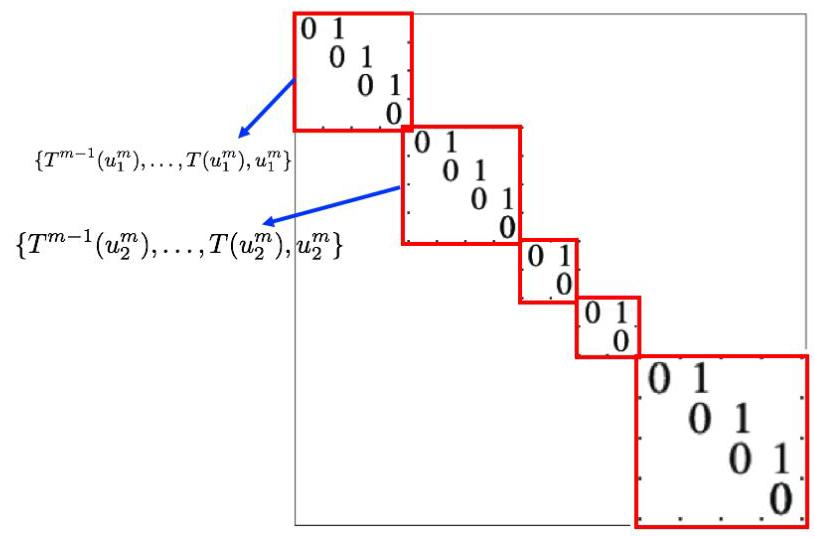
\includegraphics[max width=0.6\textwidth]{images/bo_d1h964v7aajc7382l5mg_118_410_600_815_537_0.jpg}
\end{center}
\hspace*{3em} 

Figure 9.2: Illustration for \({\left( T\right) }_{\mathcal{A},\mathcal{A}}\)

Then we consider the case where \({m}_{T}\left( x\right)  = {\left( x - \lambda \right) }^{e}\) :

Corollary 9.3 Suppose \(T : V \rightarrow  V\) is such that \({m}_{T}\left( x\right)  = {\left( x - \lambda \right) }^{e}\), then the theorem (9.3) holds, i.e., there exists a basis \(\mathcal{A}\) such that

\[
{\left( T\right) }_{\mathcal{A},\mathcal{A}} = \operatorname{diag}\left( {{J}_1,\ldots ,{J}_{\ell }}\right) ,
\]

where each block \({J}_{i}\) is a square matrix of the form

\[
{J}_{i} = \left\lbrack  \begin{matrix} \lambda & 1 & & \\   & \lambda &  \ddots  & \\   & &  \ddots  & 1 \\   & & & \lambda  \end{matrix}\right\rbrack  .
\]

Proof. Suppose that \({m}_{T}\left( x\right)  = {\left( x - \lambda \right) }^{e}\). Consider the operator \(U \mathrel{\text{ := }} T - {\lambda I}\), then \({m}_{U}\left( x\right)  = {x}^{e}\).

By applying proposition (9.6),

\[
{\left( U\right) }_{\mathcal{A},\mathcal{A}} = \operatorname{diag}\left( {{\mathbf{J}}_1,\ldots ,{\mathbf{J}}_{\ell }}\right) ,
\]

where

\[
{J}_{i} = \left\lbrack  \begin{matrix} 0 & 1 & & \\   & 0 &  \ddots  & \\   & &  \ddots  & 1 \\   & & & 0 \end{matrix}\right\rbrack  .
\]

Or equivalently,

\[
{\left( T\right) }_{\mathcal{A},\mathcal{A}} - \lambda {\left( I\right) }_{\mathcal{A},\mathcal{A}} = \operatorname{diag}\left( {{\mathbf{J}}_1,\ldots ,{\mathbf{J}}_{\ell }}\right)
\]

i.e.,

\[
{\left( T\right) }_{\mathcal{A},\mathcal{A}} = \operatorname{diag}\left( {{\mathbf{K}}_1,\ldots ,{\mathbf{K}}_{\ell }}\right) ,
\]

where

\[
{\mathbf{K}}_{i} = \left\lbrack  \begin{matrix} \lambda & 1 & & \\   & \lambda &  \ddots  & \\   & &  \ddots  & 1 \\   & & & \lambda  \end{matrix}\right\rbrack
\]

\(\mathbb{R}\) The Jordan Normal Form Theorem (9.3) follows from our arguments using the primary decomposition.

Corollary 9.4 Any matrix \(A \in  {M}_{n \times  n}\left( \mathbb{C}\right)\) is similar to a matrix of the Jordan normal form

\[
\operatorname{diag}\left( {{\mathbf{J}}_1,\ldots ,{\mathbf{J}}_{\ell }}\right) \text{ . }
\]

\section*{9.4.2. Inner Product Spaces}

Definition 9.8 [Bilinear] Let \(V\) be a vector space over \(\mathbb{R}\). A bilinear form on \(V\) is a mapping

\[
F : V \times  V \rightarrow  \mathbb{R}
\]

satisfying

1. \(F\left( {\mathbf{u} + \mathbf{v},\mathbf{w}}\right)  = F\left( {\mathbf{u},\mathbf{w}}\right)  + F\left( {\mathbf{v},\mathbf{w}}\right)\)

2. \(F\left( {\mathbf{u},\mathbf{v} + \mathbf{w}}\right)  = F\left( {\mathbf{u},\mathbf{v}}\right)  + F\left( {\mathbf{u},\mathbf{w}}\right)\)

3. \(F\left( {\lambda \mathbf{u},\mathbf{v}}\right)  = {\lambda F}\left( {\mathbf{u},\mathbf{v}}\right)  = F\left( {\mathbf{u},\lambda \mathbf{v}}\right)\)

We say

\begin{itemize}
\item \(F\) is symmetric if \(F\left( {\mathbf{u},\mathbf{v}}\right)  = F\left( {\mathbf{v},\mathbf{u}}\right)\)
\end{itemize}

\begin{itemize}
\item \(F\) is non-degenerate if \(F\left( {\mathbf{u},\mathbf{w}}\right)  = \mathbf{0}\) for all \(\mathbf{u} \in  V\) implies \(\mathbf{w} = 0\)
\end{itemize}

\begin{itemize}
\item \(F\) is positive definite if \(F\left( {\mathbf{v},\mathbf{v}}\right)  > 0\) for all \(\mathbf{v} \neq  \mathbf{0}\)
\end{itemize}

If \(F\) is positive-definite, then \(F\) is non-degenerate: Suppose that \(F\left( {\mathbf{v},\mathbf{v}}\right)  >\)  \(0,\forall \mathbf{v} \neq  \mathbf{0}\). If we have \(F\left( {\mathbf{u},\mathbf{w}}\right)  = 0\) for any \(\mathbf{u} \in  V\), then in particular, when \(\mathbf{u} = \mathbf{w}\), we imply \(F\left( {\mathbf{w},\mathbf{w}}\right)  = 0\). By positive-definiteness, \(\mathbf{w} = \mathbf{0}\), i.e., \(F\) is non-degenerate.

\section*{Chapter 10}

\section*{Week10}

\section*{10.1. Monday for MAT 3040}

\section*{10.1.1. Inner Product Space}

\begin{itemize}
\item Symmetric: \(F\left( {\mathbf{u},\mathbf{w}}\right)  = F\left( {\mathbf{w},\mathbf{u}}\right) ,\forall \mathbf{u},\mathbf{w}\)
\end{itemize}

\begin{itemize}
\item Non-degenerate: \(F\left( {\mathbf{u},\mathbf{w}}\right)  = 0,\forall \mathbf{w}\) implies \(\mathbf{u} = \mathbf{0}\)
\end{itemize}

\begin{itemize}
\item Positive definite: \(F\left( {\mathbf{v},\mathbf{v}}\right)  > 0,\forall \mathbf{v} \neq  \mathbf{0}\)
\end{itemize}

Classification. When we say \(V\) be a vector space over \(\mathbb{F}\), we treat \(\alpha  \in  \mathbb{F}\) as a scalar.

Definition 10.1 [Sesqui-linear Form] Let \(V\) be a vector space over \(\mathbb{C}\). A sesquilinear form on \(V\) is a function \(F : V \times  V \rightarrow  \mathbb{C}\) such that

1. \(F\left( {\mathbf{u} + \mathbf{v},\mathbf{w}}\right)  = F\left( {\mathbf{u},\mathbf{w}}\right)  + F\left( {\mathbf{v},\mathbf{w}}\right)\)

2. \(F\left( {\mathbf{u},\mathbf{v} + \mathbf{w}}\right)  = F\left( {\mathbf{u},\mathbf{v}}\right)  + F\left( {\mathbf{u},\mathbf{w}}\right)\)

3. \(F\left( {\bar{\lambda }\mathbf{v},\mathbf{w}}\right)  = F\left( {\mathbf{v},\lambda \mathbf{w}}\right)  = {\lambda F}\left( {\mathbf{v},\mathbf{w}}\right) ,\forall \lambda  \in  \mathbb{C}\)

In this case, we say \(F\) is conjugate symmetric if

\[
F\left( {\mathbf{v},\mathbf{w}}\right)  = \overline{F\left( {\mathbf{w},\mathbf{v}}\right) },\;\forall \mathbf{v},\mathbf{w} \in  V.
\]

The definition for non-degenerateness, and positve definiteness is the same as that in bilinear form.

In the sesquilinear form, why there is a \(\bar{\lambda }\) shown in condition (3)? Partial Answer: We want our \(F\) to be positive definite in many cases:

\begin{itemize}
\item Suppose that \(F\left( {\mathbf{v},\mathbf{v}}\right)  > 0\) and we do not have \(\bar{\lambda }\) in sesquilinear form \(F\), it follows that
\end{itemize}

\[
F\left( {i\mathbf{v},i\mathbf{v}}\right)  = {i}^2F\left( {\mathbf{v},\mathbf{v}}\right)  =  - F\left( {\mathbf{v},\mathbf{v}}\right)  < 0
\]

As a result, there will be no positive bilinear form for vector space over C.

Therefore, \(\bar{\lambda }\) is essential to guarantee that we have a positive definite form on vector space over \(\mathbb{C}\), i.e.,

\[
F\left( {i\mathbf{v},i\mathbf{v}}\right)  = \bar{i}{iF}\left( {\mathbf{v},\mathbf{v}}\right)  = F\left( {\mathbf{v},\mathbf{v}}\right)
\]

\begin{itemize}
\item Example 10.1 Consider \(V = {\mathbb{C}}^n\), and a basic sesquilinear form is the Hermitian inner product:
\end{itemize}

\[
F\left( {\mathbf{v},\mathbf{u}}\right)  = {\bf v}^{\mathrm{H}}\mathbf{u} = \left( \begin{array}{lll} \overline{{\bf v}_1} & \cdots & \overline{{\bf v}_n} \end{array}\right) \left( \begin{matrix} {\bf w}_1 \\  \vdots \\  {\bf w}_n \end{matrix}\right)  = \mathop{\sum }\limits_{{i = 1}}^n\overline{{\bf v}_{i}}{\bf w}_{i}
\]

In this case, we do not have symmetric property \(F\left( {\mathbf{v},\mathbf{w}}\right)  = F\left( {\mathbf{w},\mathbf{v}}\right)\) any more, instead, we have the conjugate symmetric property \(F\left( {\mathbf{v},\mathbf{w}}\right)  = \overline{F\left( {\mathbf{w},\mathbf{v}}\right) }\).

Definition 10.2 [Inner Product] A real (complex) vector space \(V\) with a bilinear (sesquilin-ear) form with symmetric (conjugate symmetric) and positive definite property is called an inner product on \(V\). Any vector space equipped with inner product is called an inner product space.

Notation. We write \(\langle  \cdot  , \cdot  \rangle\) instead of \(F\left( {\cdot , \cdot  }\right)\) to denote inner product.

Definition 10.3 [Norm] The norm of a vector \(\mathbf{v}\) is \(\parallel \mathbf{v}\parallel  = \sqrt{\langle \mathbf{v},\mathbf{v}\rangle }\).

As a result, \(\parallel \alpha \mathbf{v}\parallel  = \sqrt{\langle \alpha \mathbf{v},\alpha \mathbf{v}\rangle } = \sqrt{\bar\alpha\alpha \langle \mathbf{v},\mathbf{v}\rangle } = \sqrt{{\left| \alpha \right| }^2\langle \mathbf{v},\mathbf{v}\rangle } = \left| \alpha \right| \parallel \mathbf{v}\parallel\).

The norm is well-defined since \(\langle \mathbf{v},\mathbf{v}\rangle  \geq  0\) (positive definiteness of inner product).

Definition 10.4 [Orthogonal] We say a family of vectors \(S = \left\{  {{\bf v}_{i} \mid  i \in  I}\right\}\) is orthogonal if

\[
\left\langle  {{\bf v}_{i},{\bf v}_{j}}\right\rangle   = 0,\forall i \neq  j
\]

If furthermore \(\left\langle  {{\bf v}_{i},{\bf v}_{i}}\right\rangle   = 1,\forall i\), then we say \(S\) is an orthonormal set.

1. The Cauchy-Scharwz inequality holds for inner product space:

\[
\left| {\langle \mathbf{u},\mathbf{v}\rangle }\right|  \leq  \parallel \mathbf{u}\parallel \parallel \mathbf{v}\parallel ,\forall \mathbf{u},\mathbf{v} \in  V.
\]

Proof. The proof for \(\langle \mathbf{u},\mathbf{v}\rangle  \in  \mathbb{R}\) is the same as in MAT 2040 course. Check

Theorem (6.1) in the note

https://walterbabyrudin.github.io/information/Notes/MAT 2040.pdf

However, for \(\langle \mathbf{u},\mathbf{v}\rangle  \in  \mathbb{C} \smallsetminus  \mathbb{R}\), we need the re-scaling technique:

Let \(\mathbf{w} = \frac1{\langle \mathbf{u},\mathbf{v}\rangle }\mathbf{u}\), then \(\langle \mathbf{w},\mathbf{v}\rangle  \in  \mathbb{R}\) :

\[
\langle \mathbf{w},\mathbf{v}\rangle  = \left\langle  {\frac1{\langle \mathbf{u},\mathbf{v}\rangle }\mathbf{u},\mathbf{v}}\right\rangle   = \overline{\left( \frac1{\overline{\langle \mathbf{u},\mathbf{v}\rangle }}\right) }\langle \mathbf{u},\mathbf{v}\rangle  = \frac1{\langle \mathbf{u},\mathbf{v}\rangle }\langle \mathbf{u},\mathbf{v}\rangle  = 1.
\]

Applying the Cauchy-Scharwz inequality for \(\langle \mathbf{w},\mathbf{v}\rangle  \in  \mathbb{R}\) gives

\[
\left| \left\langle  {\frac1{\langle \mathbf{u},\mathbf{v}\rangle }\mathbf{u},\mathbf{v}}\right\rangle  \right|  = \left| {\langle \mathbf{w},\mathbf{v}\rangle }\right|
\]

\[
\leq  \parallel \mathbf{w}\parallel \parallel \mathbf{v}\parallel  = \begin{Vmatrix}{\frac1{\overline{\langle \mathbf{u},\mathbf{v}\rangle }}\mathbf{u}}\end{Vmatrix}\parallel \mathbf{v}\parallel
\]

Or equivalently,

\[
\left| \frac1{\langle \mathbf{u},\mathbf{v}\rangle }\right| \left| {\langle \mathbf{u},\mathbf{v}\rangle }\right|  \leq  \left| \frac1{\overline{\langle \mathbf{u},\mathbf{v}\rangle }}\right| \parallel \mathbf{u}\parallel \parallel \mathbf{v}\parallel
\]

Since \(\left| \frac1{\langle \mathbf{u},\mathbf{v}\rangle }\right|  = \left| \frac1{\langle \mathbf{u},\mathbf{v}\rangle }\right|\), we imply

\[
\left| {\langle \mathbf{u},\mathbf{v}\rangle }\right|  \leq  \parallel \mathbf{u}\parallel \parallel \mathbf{v}\parallel
\]

2. The triangle inequality also holds for inner product process:

\[
\parallel \mathbf{u} + \mathbf{v}\parallel  \leq  \parallel \mathbf{u}\parallel  + \parallel \mathbf{v}\parallel
\]

3. The Gram-Schmidt process holds for finite set of vectors: let \(S = \left\{  {{\bf v}_1,\ldots ,{\bf v}_n}\right\}\) be (finite) linearly independent. Then we can construct an orthonormal set from \(S\) :

\[
{\bf w}_1 = {\bf v}_1,\;{\bf w}_{i + 1} = {\bf v}_{i + 1} - \frac{\left\langle  {\bf v}_{i + 1},{\bf w}_1\right\rangle  }{{\begin{Vmatrix}{\bf w}_1\end{Vmatrix}}^2} - \frac{\left\langle  {\bf v}_{i + 1},{\bf w}_2\right\rangle  }{{\begin{Vmatrix}{\bf w}_2\end{Vmatrix}}^2} - \cdots  - \frac{\left\langle  {\bf v}_{i + 1},{\bf w}_{i}\right\rangle  }{{\begin{Vmatrix}{\bf w}_{i}\end{Vmatrix}}^2},i = 1,\ldots ,n - 1
\]

Then after normalization, we obtain the constructed orthonormal set. Consequently, every finite dimensional inner product space has an orthonormal basis.

\section*{10.1.2. Dual spaces}

Theorem 10.1 - Riesz Representation. Consider the mapping

\[
\phi  : \;V \rightarrow  {V}^{ * }
\]

\[
\text{ with }\mathbf{v} \mapsto  {\phi }_{\bf v}
\]

\[
\text{ where }{\phi }_{v}\left( w\right)  = \langle v,w\rangle ,\forall w \in  V
\]

Then the mapping \(\phi\) is well-defined and it is an \(\mathbb{R}\) -linear transformation.

Moreover, if \(V\) is finite dimensional, then \(\phi\) is an isomorphism.

The \(\mathbb{R}\) -linear transformation \(V \rightarrow  {V}^{ * }\) means that, when \(V,{V}^{ * }\) are vector space over \(\mathbb{R}\), the \(\mathbb{R}\) -linear transformation deduces into exactly the linear transformation.

The \(\mathbb{R}\) -linear transformation \(V \rightarrow  {V}^{ * }\) is not necessarily linear if \(V,{V}^{ * }\) are vector spaces over \(\mathbb{C}\).

However, we can transform a vector space over \(\mathbb{C}\) into a vector space over \(\mathbb{R}\) :

\begin{itemize}
\item For example, suppose that \(\left\{  {{\bf v}_1,\ldots ,{\bf v}_n}\right\}\) is a basis of \(V\) over \(\mathbb{C}\), i.e.,
\end{itemize}

\[
\mathbf{v} = \mathop{\sum }\limits_{{j = 1}}^n\alpha_{j}{\bf v}_{j}
\]

where \(\alpha_{j} = {p}_{j} + i{q}_{j},\forall {p}_{j},{q}_{j} \in  \mathbb{R}\), then

\[
\mathbf{v} = \mathop{\sum }\limits_{j}{p}_{j}{\bf v}_{j} + \mathop{\sum }\limits_{j}{q}_{j}\left( {i{\bf v}_{j}}\right) ,{p}_{j},{q}_{j} \in  \mathbb{R}
\]

Therefore, \(\left\{  {{\bf v}_1,\ldots ,{\bf v}_n,i{\bf v}_1,\ldots ,i{\bf v}_n}\right\}\) forms a basis of \(V\) over \(\mathbb{R}\).

Note that \(i{\bf v}_1\) cannot be considered as a linear combination of \({\bf v}_1\) over \(\mathbb{R}\), but a linear combination of \({\bf v}_1\) over \(\mathbb{C}\). In particular, if \(\phi  : V \rightarrow  {V}^{ * }\) is a \(\mathbb{R}\) -linear transformation, then

\[
\phi \left( {i\mathbf{v}}\right)  \neq  {i\phi }\left( \mathbf{v}\right) \text{ , but }\phi \left( {2\mathbf{v}}\right)  = {2\phi }\left( \mathbf{v}\right) \text{ . }
\]

Proof. 1. Well-definedness: We need to show \({\phi }_{v} \in  {V}^{ * }\), i.e., for scalars \(a,b\),

\[
{\phi }_{\bf v}\left( {a{\bf w}_1 + b{\bf w}_2}\right)  = \left\langle  {\mathbf{v},a{\bf w}_1 + b{\bf w}_2}\right\rangle   = a\left\langle  {\mathbf{v},{\bf w}_1}\right\rangle   + b\left\langle  {\mathbf{v},{\bf w}_2}\right\rangle   = a{\phi }_{\bf v}\left( {\bf w}_1\right)  + b{\phi }_{\bf v}\left( {\bf w}_2\right)
\]

Therefore, \({\phi }_{v} \in  {V}^{ * }\). 2. \(\mathbb{R}\) -linearity of \(\phi\) : it suffices to show

\[
\phi \left( {c{\bf v}_1 + d{\bf v}_2}\right)  = {c\phi }\left( {\bf v}_1\right)  + {d\phi }\left( {\bf v}_2\right) ,\;\forall c,d \in  \mathbb{R},{\bf v}_1,{\bf v}_2 \in  V.
\]

For all \(w \in  V\), we have

\[
{\phi }_{c{\bf v}_1 + d{\bf v}_2}\left( \mathbf{w}\right)  = \left\langle  {c{\bf v}_1 + d{\bf v}_2,\mathbf{w}}\right\rangle   = c\left\langle  {{\bf v}_1,\mathbf{w}}\right\rangle   + d\left\langle  {{\bf v}_2,\mathbf{w}}\right\rangle   = c{\phi }_{{\bf v}_1}\left( \mathbf{w}\right)  + d{\phi }_{{\bf v}_2}\left( \mathbf{w}\right)
\]

where the second equality holds because \(c,d \in  \mathbb{R}\).

Therefore,

\[
\phi \left( {c{\bf v}_1 + d{\bf v}_2}\right)  = {c\phi }\left( {\bf v}_1\right)  + {d\phi }\left( {\bf v}_2\right) .
\]

\section*{10.4. Wednesday for MAT 3040}

Reviewing. Consider the mapping

\[
\phi  : \;V \rightarrow  {V}^{ * }
\]

\[
\text{ with }\phi \left( \mathbf{v}\right)  = {\phi }_{\bf v}
\]

\[
\text{ where }{\phi }_{\bf v}\left( \mathbf{w}\right)  = \langle \mathbf{v},\mathbf{w}\rangle
\]

The Riesz Representation Theorem claims that

1. \(\phi\) is a \(\mathbb{R}\) -linear transformation.

2. \(\phi\) is injective.

3. If \(\dim \left( V\right)  < \infty\), then \(\phi\) is an isomorphism.

Proof for Claim (2). Consider the equality \(\phi \left( \mathbf{v}\right)  = {\phi }_{\bf v} = {0}_{{V}^{ * }}\), which implies

\[
{\phi }_{\bf v}\left( \mathbf{w}\right)  = \langle \mathbf{v},\mathbf{w}\rangle  = 0,\forall \mathbf{w} \in  V
\]

By the non-degenercy property, \(v = {0}_{v}\), i.e., \(\phi\) is injective.

Proof for Claim (3). Since \({\dim }_{\mathbb{R}}\left( V\right)  = {\dim }_{\mathbb{R}}\left( {V}^{ * }\right)\), and \(\phi\) is injective as a \(\mathbb{R}\) -linear transformation, we imply \(\phi\) is an isomorphism from \(V\) to \({V}^{ * }\), where \(V,{V}^{ * }\) are treated as vector spaces over \(\mathbb{R}\).

\section*{10.4.1. Orthogonal Complement}

Definition 10.5 [Orthogonal Complement] Let \(U \leq  V\) be a subspace of an inner product space. Then the orthogonal complement of \(U\) is

\[
{U}^{ \bot  } = \{ \mathbf{v} \in  V \mid  \langle \mathbf{v},\mathbf{u}\rangle  = 0,\forall \mathbf{u} \in  U\}
\]

The analysis for orthogonal complement for vector spaces over \(\mathbb{C}\) is quite similar as what we have studied in MAT 2040.

Proposition \({10.7}\;1.{U}^{ \bot  }\) is a subspace of \(V\)

2. \(U \cap  {U}^{ \bot  } = \{ 0\}\)

3. \({U}_1 \subseteq  {U}_2\) implies \({U}_2^{ \bot  } \leq  {U}_1^{ \bot  }\).

Proof. 1. Suppose that \({\bf v}_1,{\bf v}_2 \in  {U}^{ \bot  }\), where \(a,b \in  K\left( {K = \mathbb{C}\text{ or }\mathbb{R}}\right)\), then for all \(\mathbf{u} \in  U\),

\[
\left\langle  {a{\bf v}_1 + b{\bf v}_2,\mathbf{u}}\right\rangle   = \bar{a}\left\langle  {{\bf v}_1,\mathbf{u}}\right\rangle   + \bar{b}\left\langle  {{\bf v}_2,\mathbf{u}}\right\rangle
\]

\[
= \bar{a} \cdot  0 + \bar{b} \cdot  0 = 0
\]

Therefore, \(a{\bf v}_1 + b{\bf v}_2 \in  {U}^{ \bot  }\).

2. Suppose that \(\mathbf{u} \in  U \cap  {U}^{ \bot  }\), then we imply \(\langle \mathbf{u},\mathbf{u}\rangle  = 0\). By the positive-definiteness of inner product, \(\mathbf{u} = \mathbf{0}\).

3. The statement (3) is easy.

Proposition 10.8 1. If \(\dim \left( V\right)  < \infty\) and \(U \leq  V\), then \(V = U \oplus  {U}^{ \bot  }\)

2. If \(U,W \leq  V\), then

\[
{\left( U + W\right) }^{ \bot  } = {U}^{ \bot  } \cap  {W}^{ \bot  }
\]

\[
{\left( U \cap  W\right) }^{ \bot  } \supseteq  {U}^{ \bot  } + {W}^{ \bot  }
\]

\[
{\left( {U}^{ \bot  }\right) }^{ \bot  } \supseteq  U
\]

Moreover, if \(\dim \left( V\right)  < \infty\), then these are equalities.

Proof. 1. Suppose that \(\left\{  {{\bf v}_1,\ldots ,{\bf v}_{k}}\right\}\) forms a basis for \(U\), and by basis extension, we obtain \(\left\{  {{\bf v}_1,\ldots ,{\bf v}_{k},{\bf v}_{k + 1},\ldots ,{\bf v}_n}\right\}\) is a basis for \(V\).

By Gram-Schmidt Process, any finite basis induces an orthonormal basis. Therefore, suppose that \(\left\{  {{\mathbf{e}}_1,\ldots ,{\mathbf{e}}_{k}}\right\}\) forms an orthonormal basis for \(U\), and \(\left\{  {{\mathbf{e}}_{k + 1},\ldots ,{\mathbf{e}}_n}\right\}\) forms an orthonormal basis for \({U}^{ \bot  }\).

It’s easy to show \(V = U + {U}^{ \bot  }\) using orthonormal basis.

2. (a) The reverse part \({\left( U + W\right) }^{ \bot  } \supseteq  {U}^{ \bot  } \cap  {W}^{ \bot  }\) is trivial; for the forward part, suppose

\(v \in  {\left( U + W\right) }^{ \bot  }\), then

\[
\langle \mathbf{v},\mathbf{u} + \mathbf{w}\rangle  = 0,\forall \mathbf{u} \in  U,\mathbf{w} \in  W
\]

Taking \(\mathbf{u} \equiv  \mathbf{0}\) in the equality above gives \(\langle \mathbf{v},\mathbf{w}\rangle  = 0\), i.e., \(\mathbf{v} \in  {U}^{ \bot  }\). Similarly, \(v \in  {W}^{ \bot  }\).

(b) Follow the similar argument as in (2a). If \(\dim \left( V\right)  < \infty\), then write down the orthonormal basis for \({U}^{ \bot  } + {W}^{ \bot  }\) and \({\left( U \cap  W\right) }^{ \bot  }\).

(c) Follow the similar argument as in (2a). If \(\dim \left( V\right)  < \infty\), then

\[
V = {U}^{ \bot  } \oplus  {\left( {U}^{ \bot  }\right) }^{ \bot  } = U \oplus  {U}^{ \bot  }.
\]

Therefore, \({\left( {U}^{ \bot  }\right) }^{ \bot  } = U\).

Proposition 10.9 The mapping \(\phi  : V \rightarrow  {V}^{ * }\) maps \({U}^{ \bot  } \leq  V\) injectively to \(\operatorname{Ann}\left( U\right)  \leq  {V}^{ * }\). If \(\dim \left( V\right)  < \infty\), then \({U}^{ \bot  } \cong  \operatorname{Ann}\left( U\right)\) as \(\mathbb{R}\) -vector spaces

Proof. The injectivity of \(\phi\) has been shown at the beginning of this lecture. For any \(\mathbf{v} \in  {U}^{ \bot  }\), we imply \({\phi }_{\bf v}\left( \mathbf{u}\right)  = 0,\forall \mathbf{u} \in  U\), i.e., \({\phi }_{\bf v} \in  \operatorname{Ann}\left( U\right)\).

Therefore, \(\phi \left( {U}^{ \bot  }\right)  \leq  \operatorname{Ann}\left( U\right)\).

Provided that \(\dim \left( V\right)  < \infty\), by (1) in proposition (10.8),

\[
\dim \left( U\right)  + \dim \left( {U}^{ \bot  }\right)  = \dim \left( V\right)
\]

Since \(\dim \left( U\right)  + \dim \left( {\operatorname{Ann}\left( U\right) }\right)  = \dim \left( V\right)\), we imply \(\dim \left( {U}^{ \bot  }\right)  = \dim \left( {\operatorname{Ann}\left( U\right) }\right)\).

Moreover,

\[
\phi  : {U}^{ \bot  } \rightarrow  \operatorname{Ann}\left( U\right)
\]

is an isomorphism between \(\mathbb{R}\) -vector spaces \({U}^{ \bot  }\) and \(\operatorname{Ann}\left( U\right)\).

\section*{10.4.2. Adjoint Map}

Motivation. Then we study the induced mapping based on a given linear operator \(T\), denoted as \({T}^{\prime }\). This induced mapping essentially plays the similar role as taking the Hermitian for a complex matrix.

Notation. Previously we have studied the adjoint of \(T : V \rightarrow  W\), denoted as \({T}^{ * } : {W}^{ * } \rightarrow\)  \({V}^{ * }\). However, from now on, we use the same terminalogy but with different meaning. If \(T : V \rightarrow  V\) is a linear operator, then the adjoint of \(T\) is the linear operator \({T}^{\prime } : V \rightarrow  V\) defined as follows.

Definition 10.6 [Adjoint] Let \(T : V \rightarrow  V\) be a linear operator between inner product spaces. The adjoint of \(T\) is defined as \({T}^{\prime } : V \rightarrow  V\) satisfying

\[
\left\langle  {{T}^{\prime }\left( \mathbf{v}\right) ,\mathbf{w}}\right\rangle   = \langle \mathbf{v},T\left( \mathbf{w}\right) \rangle ,\forall \mathbf{w} \in  V \tag{10.1}
\]

Proposition 10.10 If \(\dim \left( V\right)  < \infty\), then \({T}^{\prime }\) exists, and it is unique. Moreove, \({T}^{\prime }\) is a linear map.

Proof. Fix any \(v \in  V\). Consider the mapping

\[
\alpha_{\bf v} : \mathbf{w}\overset{T}{ \rightarrow  }T\left( \mathbf{w}\right) \overset{{\phi }_{\bf v}}{ \rightarrow  }\langle \mathbf{v},T\left( \mathbf{w}\right) \rangle
\]

This is a linear transformation from \(V\) to \(\mathbb{F}\), i.e., \(\alpha_{v} \in  {V}^{ * }\)

By Riesz representation theorem, \(\phi\) is an isomorphism from \(V\) to \({V}^{ * }\). Therefore, for any \(\alpha_{v} \in  {V}^{ * }\), there exists a vector \({T}^{\prime }\left( v\right)  \in  V\) such that

\[
\phi \left( {{T}^{\prime }\left( \mathbf{v}\right) }\right)  = \alpha_{\bf v} \in  {V}^{ * }
\]

Or equivalently, \({\phi }_{{T}^{\prime }\left( \mathbf{v}\right) }\left( \mathbf{w}\right)  = \alpha_{\bf v}\left( \mathbf{w}\right) ,\forall \mathbf{w} \in  V\), i.e., \(\left\langle  {{T}^{\prime }\left( \mathbf{v}\right) ,\mathbf{w}}\right\rangle   = \langle \mathbf{v},T\left( \mathbf{w}\right) \rangle\).

Therefore, from \(v\) we have constructed \({T}^{\prime }\left( v\right)\) satisfying (10.1). Now define \({T}^{\prime } : V \rightarrow  V\) by \(v \mapsto  {T}^{\prime }\left( v\right)\).

\begin{itemize}
\item Since the choice of \({T}^{\prime }\left( v\right)\) is unique by the injectivity of \(\phi ,{T}^{\prime }\) is well-defined.
\end{itemize}

\begin{itemize}
\item Now we show \({T}^{\prime }\) is a linear transformation: Let \({\bf v}_1,{\bf v}_2 \in  V,a,b \in  K\). For all \(\mathbf{w} \in  V\),
\end{itemize}

we have

\[
\left\langle  {{T}^{\prime }\left( {a{\bf v}_1 + b{\bf v}_2}\right) ,\mathbf{w}}\right\rangle   = \left\langle  {a{\bf v}_1 + b{\bf v}_2,T\left( \mathbf{w}\right) }\right\rangle
\]

\[
= \bar{a}\left\langle  {{\bf v}_1,T\left( \mathbf{w}\right) }\right\rangle   + \bar{b}\left\langle  {{\bf v}_2,T\left( \mathbf{w}\right) }\right\rangle
\]

\[
= \bar{a}\left\langle  {{T}^{\prime }\left( {\bf v}_1\right) ,\mathbf{w}}\right\rangle   + \bar{b}\left\langle  {{T}^{\prime }\left( {\bf v}_2\right) ,\mathbf{w}}\right\rangle
\]

\[
= \left\langle  {a{T}^{\prime }\left( {\bf v}_1\right)  + b{T}^{\prime }\left( {\bf v}_2\right) ,\mathbf{w}}\right\rangle
\]

Therfore,

\[
\left\langle  {{T}^{\prime }\left( {a{\bf v}_1 + b{\bf v}_2}\right)  - \left\lbrack  {a{T}^{\prime }\left( {\bf v}_1\right)  + b{T}^{\prime }\left( {\bf v}_2\right) }\right\rbrack  ,\mathbf{w}}\right\rangle   = 0,\forall \mathbf{w} \in  V
\]

By the non-degeneracy of inner product,

\[
{T}^{\prime }\left( {a{\bf v}_1 + b{\bf v}_2}\right)  - \left\lbrack  {a{T}^{\prime }\left( {\bf v}_1\right)  + b{T}^{\prime }\left( {\bf v}_2\right) }\right\rbrack   = \mathbf{0},
\]

i.e., \({T}^{\prime }\left( {a{\bf v}_1 + b{\bf v}_2}\right)  = a{T}^{\prime }\left( {\bf v}_1\right)  + b{T}^{\prime }\left( {\bf v}_2\right)\)

\begin{itemize}
\item Example 10.2 Let \(V = {\mathbb{R}}^n,\langle  \cdot  , \cdot  \rangle\) as the usual inner product. Consider the matrix-multiplication mapping
\end{itemize}

\[
T : \;V \rightarrow  V
\]

\[
T\left( \mathbf{v}\right)  = A\mathbf{v}
\]

Then \(\left\langle  {{T}^{\prime }\left( \mathbf{v}\right) ,\mathbf{w}}\right\rangle   = \langle \mathbf{v},T\left( \mathbf{w}\right) \rangle\) implies

\[
{\left( {T}^{\prime }\left( \mathbf{v}\right) \right) }^{\mathrm{T}}\mathbf{w} = \langle \mathbf{v},A\mathbf{w}\rangle
\]

\[
= {v}^{\mathrm{T}}{Aw}
\]

\[
= {\left( {A}^{\mathrm{T}}\mathbf{v}\right) }^{\mathrm{T}}\mathbf{w}
\]

Therfore, \({T}^{\prime }\left( \mathbf{v}\right)  = {A}^{\mathrm{T}}\mathbf{v}\). Proposition 10.11 Let \(T : V \rightarrow  V\) be a linear transformation, \(V\) a inner product space.

Suppose that \(\mathcal{B} = \left\{  {{\mathbf{e}}_1,\ldots ,{\mathbf{e}}_n}\right\}\) is an orthonormal basis of \(V\), then

\[
{\left( {T}^{\prime }\right) }_{\mathcal{B},\mathcal{B}} = \overline{{\left( {\left( T\right) }_{\mathcal{B},\mathcal{B}}\right) }^{\mathrm{T}}}
\]

Proof. Suppose that \({\left( T\right) }_{\mathcal{B},\mathcal{B}} = \left( {a}_{ij}\right)\), where \(T\left( {\mathbf{e}}_{j}\right)  = \mathop{\sum }\limits_{{k = 1}}^n{a}_{kj}{\mathbf{e}}_{k}\), then

\[
\left\langle  {{\mathbf{e}}_{i},T\left( {\mathbf{e}}_{j}\right) }\right\rangle   = \left\langle  {{\mathbf{e}}_{i},\mathop{\sum }\limits_{{k = 1}}^n{a}_{kj}{\mathbf{e}}_{k}}\right\rangle
\]

\[
= \mathop{\sum }\limits_{{k = 1}}^n{a}_{kj}\left\langle  {{\mathbf{e}}_{i},{\mathbf{e}}_{k}}\right\rangle
\]

\[
= {a}_{ij}
\]

Also, suppose \({\left( {T}^{\prime }\right) }_{\mathcal{B},\mathcal{B}} = \left( {b}_{ij}\right)\), we imply \({T}^{\prime }\left( {\mathbf{e}}_{j}\right)  = \mathop{\sum }\limits_{{k = 1}}^n{b}_{ij}{\mathbf{e}}_{k}\), which follows that

\[
\left\langle  {{\mathbf{e}}_{i},{T}^{\prime }\left( {\mathbf{e}}_{j}\right) }\right\rangle   = {b}_{ij} \Rightarrow  \overline{\left\langle  {T}^{\prime }\left( {\mathbf{e}}_{j}\right) ,{\mathbf{e}}_{i}\right\rangle  } = {b}_{ij} \Rightarrow  \overline{\left\langle  {\mathbf{e}}_{j},T\left( {\mathbf{e}}_{i}\right) \right\rangle  } = {b}_{ij},
\]

i.e., \(\overline{{a}_{ji}} = {b}_{ij}\).

Proposition (10.11) does not hold if \(\mathcal{B}\) is not an orthonormal basis.

\newpage
\section{Week 11}

\subsection{Self-Adjoint Operator}

\begin{definition}[Self-Adjoint Operator] Let \(V\) be an inner product space and \(T : V \rightarrow  V\) be a linear operator. Then \(T\) is {\bf self-adjoint} if \({T}^{\prime } = T\).
\end{definition}

\begin{example} 11.1 Let \(V = {\mathbb{C}}^n\), and \(\mathcal{B} = \left\{  {{\mathbf{e}}_1,\ldots ,{\mathbf{e}}_n}\right\}\) be an orthonormal basis of $V$. Let \(T : V \rightarrow  V\) be defined by
\[
T\left( \mathbf{v}_j\right)  = \sum_{i=1}^n A_{ij}\mathbf{v}_i,\;\text{ where }A \in  {M}_{n \times  n}\left( \mathbb{C}\right) .
\]
(equivalently, the matrix representation satisfies \({\left( T\right) }_{\mathcal{B},\mathcal{B}}  = A\)).
Then \(T\) is self-adjoint if and only if \({\left( {T}^{\prime }\right) }_{\mathcal{B},\mathcal{B}} = {\left( T\right) }_{\mathcal{B},\mathcal{B}}\), i.e., \(\overline{{\left( T\right) }_{\mathcal{B},\mathcal{B}}^{t}} = {\left( T\right) }_{\mathcal{B},\mathcal{B}}\), which is equivalent to 
\[A^{\mathrm{H}} = A,\]
i.e. $A$ is a Hermitian matrix (as in MAT 2040). Moreover, if \(\mathbb{C}\) is replaced by \(\mathbb{R}\), then \(T\) is self-adjoint if and only if \(A^t =A\) is a symmetric matrix. 
\end{example}

As we saw in the previous example, self-adjointness for linear operators is the generalization of Hermitian matrices in MAT 2040. Under such perspective, we would expect self-adjoint have similar nice properties as in the case of Hermitian matrices.

\begin{proposition} If \(\lambda\) is an eigenvalue of a self-adjoint operator \(T\), then \(\lambda  \in  \mathbb{R}\).
\end{proposition}

\begin{proof} Suppose there is an eigen-pair \(\left( {\lambda ,\mathbf{w}}\right)\) for \(\mathbf{w} \neq  \mathbf{0}\), then
\[
\lambda \langle \mathbf{w},\mathbf{w}\rangle  = \langle \mathbf{w},\lambda \mathbf{w}\rangle = \langle \mathbf{w},T\left( \mathbf{w}\right) \rangle  = \left\langle  {{T}^{\prime }\left( \mathbf{w}\right) ,\mathbf{w}}\right\rangle = \langle T\left( \mathbf{w}\right) ,\mathbf{w}\rangle  = \langle \lambda \mathbf{w},\mathbf{w}\rangle = \bar{\lambda }\langle \mathbf{w},\mathbf{w}\rangle
\]
Since \(\langle \mathbf{w},\mathbf{w}\rangle  \neq  0\) by non-degeneracy, we have \(\lambda  = \bar{\lambda }\), i.e., \(\lambda  \in  \mathbb{R}\).
\end{proof}


\begin{proposition} If \(U \leq  V\) is \(T\) -invariant over the self-adjoint operator \(T\), then so is \({U}^{ \bot  }\).
\end{proposition}

\begin{proof} It suffices to show \(T\left( \mathbf{v}\right)  \in  {U}^{ \bot  },\forall \mathbf{v} \in  {U}^{ \bot  }\), i.e., for any \(\mathbf{u} \in  U\), check that
\[
\langle \mathbf{u},T\left( \mathbf{v}\right) \rangle  = \left\langle  {{T}^{\prime }\left( \mathbf{u}\right) ,\mathbf{v}}\right\rangle   = \langle T\left( \mathbf{u}\right) ,\mathbf{v}\rangle  = 0,
\]
where the last equality is due to the fact that \(T\left( \mathbf{u}\right)  \in  U\) and \(\mathbf{v} \in  {U}^{ \bot  }\). Therefore, \(T\left( \mathbf{v}\right)  \in  {U}^{ \bot  }\).
\end{proof}

\begin{theorem} If \(T : V \rightarrow  V\) is self-adjoint, and \(\dim \left( V\right)  < \infty\), then there exists an orthonormal basis of eigenvectors of \(T\), i.e., an orthonormal basis of \(V\) such that any element from this basis is an eigenvector of \(T\).
\end{theorem}

\begin{proof} We use induction on \(\dim \left( V\right)\) :

\begin{itemize}
\item The result is trival for \(\dim \left( V\right)  = 1\).
\end{itemize}

\begin{itemize}
\item Suppose that this theorem holds for all vector spaces \(V\) with \(\dim \left( V\right)  \leq  k\), then we want to show the theorem holds when \(\dim \left( V\right)  = k + 1\) :
\end{itemize}

Suppose that \(T : V \rightarrow  V\) is self-adjoint with \(\dim \left( V\right)  = k + 1\), then consider

\[
{\mathcal{X}}_{T}\left( x\right)  = {x}^{k + 1} + \cdots  + {a}_1x + {a}_{0},\;{a}_{i} \in  \mathbb{K}\text{ , where }\mathbb{K}\text{ denotes }\mathbb{R}\text{ or }\mathbb{C}\text{ . }
\]

\begin{itemize}
\item If \(\mathbb{K} = \mathbb{C}\), then \({\mathcal{X}}_{T}\left( x\right)\) can be decomposed as
\end{itemize}

\[
{\mathcal{X}}_{T}\left( x\right)  = \left( {x - {\lambda }_1}\right) \cdots \left( {x - {\lambda }_{k + 1}}\right)
\]

In paricular, we obtain the eigen-pair \(\left( {{\lambda }_1,\mathbf{v}}\right)\)

\begin{itemize}
\item If \(\mathbb{K} = \mathbb{R}\), i.e., we treat real number as scalars, then
\end{itemize}

\[
{\mathcal{X}}_{T}\left( x\right)  = \left( {x - {\lambda }_1}\right) \cdots \left( {x - {\lambda }_{k + 1}}\right) \text{ , where }{\lambda }_{i} \in  \mathbb{C}\text{ . }
\]

By proposition (11.1), we imply all \({\lambda }_{i}\) ’s are in \(\mathbb{R}\). Moreover, we also obtain

the eigen-pair \(\left( {{\lambda }_1,\mathbf{v}}\right)\)

Consider \(U = \operatorname{span}\{ \mathbf{v}\}\), then

\begin{itemize}
\item \(U\) is \(T\) -invariant
\end{itemize}

\(- V = U \oplus  {U}^{ \bot  }\), since \(V\) is finite dimensional

\begin{itemize}
\item \({U}^{ \bot  }\) is \(T\) -invariant.
\end{itemize}

Consider \({\left. T\right| }_{{U}^{ \bot  }}\), which is a self-adjoint operator on \({U}^{ \bot  }\), with \(\dim \left( {U}^{ \bot  }\right)  = k\).

By induction, there exists an orthonormal basis \(\left\{  {{\mathbf{e}}_2,\ldots ,{\mathbf{e}}_{k + 1}}\right\}\) of eigenvectors of

\(T{ \mid  }_{{U}^{ \bot  }}\).

Consider the basis \(\mathcal{B} = \left\{  {{\bf v}^{\prime } = \mathbf{v}/\parallel \mathbf{v}\parallel ,{\mathbf{e}}_2,\ldots ,{\mathbf{e}}_{k + 1}}\right\}\). As a result,

1. \(\mathcal{B}\) forms a basis of \(V\)

2. All \({\bf v}^{\prime },{\mathbf{e}}_{i}\) are of norm 1 eigenvectors of \(T\).

3. \(\mathcal{B}\) is an orthonormal set, e.g., \(\left\langle  {{\bf v}^{\prime },{\mathbf{e}}_{i}}\right\rangle   = 0\), where \({\bf v}^{\prime } \in  U\) and \({\mathbf{e}}_{i} \in  {U}^{ \bot  }\).

Therefore, \(\mathcal{B}\) is a basis of orthonormal eigenvectors of \(V\).
\end{proof}

\begin{corollary} If \(\dim \left( V\right)  < \infty\), and \(T : V \rightarrow  V\) is self-adjoint, then there exists orthonormal basis \(\mathcal{B}\) such that
\[
{\left( T\right) }_{\mathcal{B},\mathcal{B}} = \operatorname{diag}\left( {{\lambda }_1,\ldots ,{\lambda }_n}\right)
\]
In particular, for all real symmetric matrix \(A \in  {\mathbb{S}}^n\), there exists orthogonal matrix \(P\left( {{P}^{\mathrm{T}}P = {\mathbf{I}}_n}\right)\) such that
\[
{P}^{-1}{AP} = \operatorname{diag}\left( {{\lambda }_1,\ldots ,{\lambda }_n}\right)
\]
\end{corollary}
\begin{proof} 1. By applying theorem (11.1), there exists orthonormal basis of \(V\), say \(\mathcal{B} =\)  \(\left\{  {{\bf v}_1,\ldots ,{\bf v}_n}\right\}\) such that \(T\left( {\bf v}_{i}\right)  = {\lambda }_{i}{\bf v}_{i}\). Directly writing the basis representation gives

\[
{\left( T\right) }_{\mathcal{B},\mathcal{B}} = \operatorname{diag}\left( {{\lambda }_1,\ldots ,{\lambda }_n}\right) .
\]

2. For the second part, consider \(T : {\mathbb{R}}^n \rightarrow  {\mathbb{R}}^n\) by \(T\left( \mathbf{v}\right)  = \mathbf{{Av}}\). Since \({A}^{\mathrm{T}} = A\), we imply \(T\) is self-adjoint. There exists orthonormal basis \(\mathcal{B} = \left\{  {{\bf v}_1,\ldots ,{\bf v}_n}\right\}\) such that

\[
{\left( T\right) }_{\mathcal{B},\mathcal{B}} = \operatorname{diag}\left( {{\lambda }_1,\ldots ,{\lambda }_n}\right) .
\]

In particular, if \(\mathcal{A} = \left\{  {{\mathbf{e}}_1,\ldots ,{\mathbf{e}}_n}\right\}\), then \({\left( T\right) }_{\mathcal{A},\mathcal{A}} = A\). We construct \(P \mathrel{\text{ := }} {\mathcal{C}}_{\mathcal{A},\mathcal{B}}\), which is the change of basis matrix from \(\mathcal{B}\) to \(\mathcal{A}\), then

\[
P = \left( \begin{array}{lll} {\bf v}_1 & \cdots & {\bf v}_n \end{array}\right)
\]

and

\[
{P}^{-1}{\left( T\right) }_{\mathcal{A},\mathcal{A}}P = {\left( T\right) }_{\mathcal{B},\mathcal{B}}
\]

Or equivalently, \({P}^{-1}{AP} = \operatorname{diag}\left( {{\lambda }_1,\ldots ,{\lambda }_n}\right)\), with

\[
{P}^{\mathrm{T}}P = \left( \begin{matrix} {\bf v}_1^{\mathrm{T}} \\  \vdots \\  {\bf v}_n^{\mathrm{T}} \end{matrix}\right) \left( \begin{array}{lll} {\bf v}_1 & \cdots & {\bf v}_n \end{array}\right)  = \mathbf{I}
\]
\end{proof}

\subsection{Orthogonal and Unitary Operators}
\begin{definition} Let \(T : V \rightarrow  V\) be a linear operator over \(\mathbb{K}\). Suppose 
\[\langle T\left( \mathbf{w}\right) ,T\left( \mathbf{v}\right) \rangle  = \langle \mathbf{w},\mathbf{v}\rangle \quad \quad \forall\ \mathbf{v},\mathbf{w} \in  V,\] 
then $T$ is called 
\begin{itemize}
    \item Orthogonal if \(\mathbb{K} = \mathbb{R}\);
    \item Unitary if \(\mathbb{K} = \mathbb{C}\).
\end{itemize}
\end{definition}

It is easy to see that \(T: V \to V\) is orthogonal or unitary if and only if \({T}^{\prime } \circ  T = I\). Namely, the reverse direction is by directly checking that
\[
\langle T\left( \mathbf{w}\right) ,T\left( \mathbf{v}\right) \rangle  = \left\langle  {{T}^{\prime } \circ  T\left( \mathbf{w}\right) ,\mathbf{v}}\right\rangle   = \langle \mathbf{w},\mathbf{v}\rangle,
\]
and the forward direction is by checking \({T}^{\prime } \circ  T\left( \mathbf{w}\right)  = \mathbf{w},\forall \mathbf{w} \in  V\) :
\[
\left\langle  {{T}^{\prime } \circ  T\left( \mathbf{w}\right) ,\mathbf{v}}\right\rangle   = \langle T\left( \mathbf{w}\right) ,T\left( \mathbf{v}\right) \rangle  = \langle \mathbf{w},\mathbf{v}\rangle  \Rightarrow  \left\langle  {{T}^{\prime } \circ  T\left( \mathbf{w}\right)  - \mathbf{w},\mathbf{v}}\right\rangle   = 0,\forall \mathbf{v} \in  V
\]
By non-degeneracy, \({T}^{\prime } \circ  T\left( \mathbf{w}\right)  - \mathbf{w} = 0\), i.e., \({T}^{\prime } \circ  T\left( \mathbf{w}\right)  = \mathbf{w},\forall \mathbf{w} \in  V\).

\begin{example} Let \(T : {\mathbb{K}}^n \rightarrow  {\mathbb{K}}^n\) be given by \(T\left( \bf v\right)  = {A\bf v}\) for some matrix $A \in M_{n \times n}(\mathbb{K})$. Then 
\begin{itemize}
\item For $\mathbb{K} = \mathbb{R}$, \(T\) is orthogonal if and only if \({A}^{\mathrm{T}}A = I\) 
\item For $\mathbb{K} = \mathbb{C}$, \(T\) is unitary if and only if \({A}^{\mathrm{H}}A = I\).
\end{itemize}
\end{example}

\begin{definition}[Orthogonal/Unitary Group]
\[
\text{ Orthognoal Group : }O\left( {n,\mathbb{R}}\right)  = \left\{  {A \in  {M}_{n \times  n}\left( \mathbb{R}\right)  \mid  {A}^{\mathrm{T}}A = I}\right\}
\]
\[
\text{ Unitary Group : }U\left( {n,\mathbb{C}}\right)  = \left\{  {A \in  {M}_{n \times  n}\left( \mathbb{C}\right)  \mid  {A}^{\mathrm{H}}A = I}\right\}
\]
\end{definition}


\begin{proposition} Let \(T : V \rightarrow  V\) be a linear operator on a vector space over \(\mathbb{K}\) satisfying \({T}^{\prime }T = I\). Then for all eigenvalues \(\lambda\) of \(T\), we have \(\left| \lambda \right|  = 1\).
\end{proposition}

\begin{proof} Suppose we have the eigen-pair \(\left( {\lambda ,\mathbf{v}}\right)\), then
\[
\langle T\mathbf{v},T\mathbf{v}\rangle  = \langle \mathbf{v},\mathbf{v}\rangle \Leftrightarrow  \langle \lambda \mathbf{v},\lambda \mathbf{v}\rangle  = \langle \mathbf{v},\mathbf{v}\rangle
\Leftrightarrow  \bar{\lambda }\lambda \langle \mathbf{v},\mathbf{v}\rangle  = \langle \mathbf{v},\mathbf{v}\rangle
\]

Since \(\langle \mathbf{v},\mathbf{v}\rangle  \neq  0\left( {\mathbf{v} \neq  \mathbf{0}}\right)\), we imply \({\left| \lambda \right| }^2 = 1\), i.e., \(\left| \lambda \right|  = 1\).
\end{proof}

\begin{proposition} Let \(T : V \rightarrow  V\) be an operator on a finite dimension \(V\) over \(\mathbb{K}\) satisfying \({T}^{\prime }T = I\). If \(U \leq  V\) is \(T\)-invariant, then \(U\) is also \({T}^{-1}\) -invariant.
\end{proposition}

\begin{proof} Since \({T}^{\prime }T = I\), i.e., \(T\) is invertible, we imply 0 is not a root of \({X}_{T}\left( x\right)\), i.e.,0 is not a root of \({m}_{T}\left( x\right)\). Since \({m}_{T}\left( 0\right)  \neq  0,{m}_{T}\left( x\right)\) has the form

\[
{m}_{T}\left( x\right)  = {x}^{m} + \cdots  + {a}_1x + {a}_{0},{a}_{0} \neq  0,
\]

which follows that

\[
{m}_{T}\left( T\right)  = {T}^{m} + \cdots  + {a}_{0}I = 0 \Rightarrow  T\left( {{T}^{m - 1} + \cdots  + {a}_1I}\right)  =  - {a}_{0}I
\]

Or equivalently,

\[
T\left( {-\frac1{{a}_{0}}\left( {{T}^{m - 1} + \cdots  + {a}_1I}\right) }\right)  = I
\]

Therefore,

\[
{T}^{-1} =  - \frac1{{a}_{0}}{T}^{m - 1} - \cdots  - \frac{{a}_2}{{a}_{0}}T - \frac{{a}_1}{{a}_{0}}I,
\]

i.e., the inverse \({T}^{-1}\) can be expressed as a polynomial involving \(T\) only.

Since \(U\) is \(T\) -invariant, we imply \(U\) is \({T}^{m}\) -invariant for \(m \in  \mathbb{N}\), and therefore \(U\) is \({T}^{-1}\) -invariant since \({T}^{-1}\) is a polynomial of \(T\).
\end{proof}

\begin{proposition} Let \(T : V \rightarrow  V\) satisfies \({T}^{\prime }T = I\left( {\dim \left( V\right)  < \infty }\right)\), then \(U \leq  V\) is \(T\) -invariant implies \({U}^{ \bot  }\) is \(T\) -invariant.
\end{proposition}

\begin{proof} Let \(v \in  {U}^{ \bot  }\), it suffices to show \(T\left( v\right)  \in  {U}^{ \bot  }\).

For all \(u \in  U\), we have

\[
\langle u,T\left( v\right) \rangle  = \left\langle  {{T}^{\prime }\left( u\right) ,v}\right\rangle   = \left\langle  {{T}^{-1}\left( u\right) ,v}\right\rangle
\]

Since \(U\) is \({T}^{-1}\) -invaraint, we imply \({T}^{-1}\left( u\right)  \in  U\), and therefore

\[
\langle u,T\left( v\right) \rangle  = \left\langle  {{T}^{-1}\left( u\right) ,v}\right\rangle   = 0 \Rightarrow  T\left( v\right)  \in  {U}^{ \bot  }.
\]
\end{proof}

\begin{theorem} Let \(T : V \rightarrow  V\) be a unitary operator on finite dimension \(V\) (over \(\mathbb{C}\)),

then there exists an orthonormal basis \(\mathcal{A}\) such that

\[
{\left( T\right) }_{\mathcal{A},\mathcal{A}} = \operatorname{diag}\left( {{\lambda }_1,\ldots ,{\lambda }_n}\right) ,\left| {\lambda }_{i}\right|  = 1,\forall i.
\]
\end{theorem}

\begin{proof} Note that \({\mathcal{X}}_{T}\left( x\right)\) always admits a root in \(\mathbb{C}\), so we can always find an eigenvector \(v \in  V\) of \(T\).

Then the theorem follows by the same argument before on seld-adjoint operators.

\begin{itemize}
\item Consider \(U = \operatorname{span}\{ \mathbf{v}\}\)
\end{itemize}

\begin{itemize}
\item \(V = U \oplus  {U}^{ \bot  }\) and \({U}^{ \bot  }\) is \(T\) -invariant
\end{itemize}

\begin{itemize}
\item Use induction on the unitary operator \({\left. T\right| }_{{U}^{ \bot  }} : {U}^{ \bot  } \rightarrow  {U}^{ \bot  }\)
\end{itemize}
\end{proof}

The argument above fails for orthogonal operators. For instance, let \(
T : \mathbb{R} \rightarrow  {\mathbb{R}}^2
\) be given by 
\[
T\left( \mathbf{v}\right)  = \left( \begin{matrix} \cos \theta &  - \sin \theta \\  \sin \theta & \cos \theta  \end{matrix}\right) \mathbf{v}
\]
The matrix \(A\) is not diagonalizable over \(\mathbb{R}\). It has no real eigenvalues. However, if we treat \(A\) as \(T : {\mathbb{C}}^2 \rightarrow  {\mathbb{C}}^2\) with \(T\left( \mathbf{v}\right)  = \mathbf{{Av}}\), then \({A}^{\mathrm{H}}A = \mathbf{I}\), and therefore \(T\) is unitary. Then \(A\) is diagonalizable over \(\mathbb{C}\) with eigenvalues \({e}^{i\theta },{e}^{-{i\theta }}\)

\begin{itemize}
\item As a corollary of the theorem, for all \(A \in  {M}_{n \times  n}\left( \mathbb{C}\right)\) satisfying \({A}^{\mathrm{H}}A = \mathbf{I}\), there exists \(P \in  {M}_{n \times  n}\left( \mathbb{C}\right)\) such that
\end{itemize}

\[
{P}^{-1}{AP} = \operatorname{diag}\left( {{\lambda }_1,\ldots ,{\lambda }_n}\right) ,\;\left| {\lambda }_{i}\right|  = 1,
\]

where \(P = \left( {{\mathbf{u}}_1,\ldots ,{\mathbf{u}}_n}\right)\), with \(\left\{  {{\mathbf{u}}_1,\ldots ,{\mathbf{u}}_n}\right\}\) forming orthonormal basis of \({\mathbb{C}}^n\). In fact,

\[
{P}^{\mathrm{H}}P = \left( \begin{matrix} {\mathbf{u}}_1^{\mathrm{H}} \\  \vdots \\  {\mathbf{u}}_n^{\mathrm{H}} \end{matrix}\right) \left( {{\mathbf{u}}_1\cdots {\mathbf{u}}_n}\right)  = \left( \begin{matrix} \left\langle  {{\mathbf{u}}_1,{\mathbf{u}}_1}\right\rangle  & \cdots & \left\langle  {{\mathbf{u}}_1,{\mathbf{u}}_n}\right\rangle  \\  \vdots &  \ddots  & \vdots \\  \left\langle  {{\mathbf{u}}_n,{\mathbf{u}}_1}\right\rangle  & \cdots & \left\langle  {{\mathbf{u}}_n,{\mathbf{u}}_n}\right\rangle   \end{matrix}\right)
\]

Conclusion: all matrices \(A \in  {M}_{n \times  n}\left( \mathbb{C}\right)\) with \({A}^{\mathrm{H}}A = \mathbf{I}\) can be written as

\[
A = {\mathbf{P}}^{-1}\operatorname{diag}\left( {{\lambda }_1,\ldots ,{\lambda }_n}\right) \mathbf{P},
\]

with some \(\mathbf{P}\) satisfying \({\mathbf{P}}^{\mathrm{H}}\mathbf{P} = \mathbf{I}\).

Notation. Let \(U\left( n\right)  = \left\{  {A \in  {M}_{n \times  n}\left( \mathbb{C}\right)  \mid  {A}^{\mathrm{H}}A = \mathbf{I})}\right\}\) be the unitary group, then all \(A \in  U\left( n\right)\) can be diagonalized by

\[
A = {P}^{-1}\operatorname{diag}\left( {{\lambda }_1,\ldots ,{\lambda }_n}\right) P,\;P \in  U\left( n\right) .
\]

\subsection{Normal Operators}
Definition 11.10 [Normal] Let \(T : V \rightarrow  V\) be a linear operator over a \(\mathbb{C}\) inner product vector space \(V\). We say \(T\) is normal, if

\[
{T}^{\prime }T = T{T}^{\prime }
\]

\begin{itemize}
\item Example 11.9 - All self-adjoint operators are normal:
\end{itemize}

\[
T = {T}^{\prime } \Rightarrow  T{T}^{\prime } = {T}^{\prime }T = {T}^2
\]

\begin{itemize}
\item All (finite-dimensional) unitary operators are normal:
\end{itemize}

\[
{T}^{\prime }T = T{T}^{\prime } = I
\]

Proposition 11.11 Let \(T\) be a normal operator on \(V\). Then

1. \(\parallel T\left( \mathbf{v}\right) \parallel  = \begin{Vmatrix}{{T}^{\prime }\left( \mathbf{v}\right) }\end{Vmatrix},\forall \mathbf{v} \in  V\).

In particular, \(T\left( \mathbf{v}\right)  = 0\) if and only if \({T}^{\prime }\left( \mathbf{v}\right)  = 0\)

2. \(\left( {T - {\lambda I}}\right)\) is also a normal operator, for any \(\lambda  \in  \mathbb{C}\)

3. \(T\left( \mathbf{v}\right)  = \lambda \mathbf{v}\) if and only if \({T}^{\prime }\left( \mathbf{v}\right)  = \bar{\lambda }\mathbf{v}\).

\begin{proof} 1.
\[
\langle T\mathbf{v},T\mathbf{v}\rangle  = \left\langle  {{T}^{\prime }T\mathbf{v},\mathbf{v}}\right\rangle
= \left\langle  {T{T}^{\prime }\mathbf{v},\mathbf{v}}\right\rangle
= \overline{\left\langle  v,T{T}^{\prime }v\right\rangle  }
= \overline{\left\langle  {T}^{\prime }\mathbf{v},{T}^{\prime }\mathbf{v}\right\rangle  }
= \left\langle  {{T}^{\prime }\mathbf{v},{T}^{\prime }\mathbf{v}}\right\rangle
\]

Therefore, \(\parallel T\left( \mathbf{v}\right) {\parallel }^2 = {\begin{Vmatrix}{T}^{\prime }\left( \mathbf{v}\right) \end{Vmatrix}}^2\), i.e., \(\parallel T\left( \mathbf{v}\right) \parallel  = \begin{Vmatrix}{{T}^{\prime }\left( \mathbf{v}\right) }\end{Vmatrix}\).

2. By hw4, \({\left( T - \lambda I\right) }^{\prime } = {T}^{\prime } - \bar{\lambda }I\). It suffices to check

\[
{\left( T - \lambda I\right) }^{\prime }\left( {T - {\lambda I}}\right)  = \left( {T - {\lambda I}}\right) {\left( T - \lambda I\right) }^{\prime },
\]

Expanding both sides out gives the desired result, i.e.,

\[
{\left( T - \lambda I\right) }^{\prime }\left( {T - {\lambda I}}\right)  = \left( {{T}^{\prime } - \bar{\lambda }I}\right) \left( {T - {\lambda I}}\right)  = {T}^{\prime }T - \bar{\lambda }T - \lambda {T}^{\prime } + \lambda \bar{\lambda }I
\]

and

\[
\left( {T - {\lambda I}}\right) {\left( T - \lambda I\right) }^{\prime } = \left( {T - {\lambda I}}\right) \left( {{T}^{\prime } - \bar{\lambda }I}\right)  = T{T}^{\prime } - \bar{\lambda }T - \lambda {T}^{\prime } + \lambda \bar{\lambda }I
\]

(3) \(\; \bullet\) For the forward direction, if \(\left( {T - {\lambda I}}\right) \mathbf{v} = 0\), then by part (2), \(\left( {T - {\lambda I}}\right)\) is normal, which follows that

\[
\begin{Vmatrix}{{\left( T - \lambda I\right) }^{\prime }\left( \mathbf{v}\right) }\end{Vmatrix} = 0 \Rightarrow  {\left( T - \lambda I\right) }^{\prime }\left( \mathbf{v}\right)  = 0 \Rightarrow  {T}^{\prime }\mathbf{v} = \bar{\lambda }\mathbf{v}.
\]

\begin{itemize}
\item For the reverse direction, suppose that \(\left( {{T}^{\prime } - \bar{\lambda }I}\right) \mathbf{v} = 0\). Since \(T\) is normal, we imply \({T}^{\prime }\) is normal. Then by part (2), \(\left( {{T}^{\prime } - \bar{\lambda }I}\right)\) is normal. By applying the same trick,
\end{itemize}

\[
{\left( {T}^{\prime } - \bar{\lambda }I\right) }^{\prime }\mathbf{v} = 0 \Rightarrow  \left( {{\left( {T}^{\prime }\right) }^{\prime } - \overline{\bar{\lambda }}I}\right) \mathbf{v} = 0.
\]

By hw \(4,{\left( {T}^{\prime }\right) }^{\prime } = T\). Therefore, \(\left( {T - {\lambda I}}\right) v = 0\).

(4) Observe that

\[
\lambda \langle \mathbf{v},\mathbf{w}\rangle  = \langle \bar{\lambda }\mathbf{v},\mathbf{w}\rangle \overset{\text{ by }\left( 3\right) }{ \Rightarrow  }\lambda \langle \mathbf{v},\mathbf{w}\rangle  = \left\langle  {{T}^{\prime }\left( \mathbf{v}\right) ,\mathbf{w}}\right\rangle   = \langle \mathbf{v},T\left( \mathbf{w}\right) \rangle  = \langle \mathbf{v},\mu \mathbf{w}\rangle  = \mu \langle \mathbf{v},\mathbf{w}\rangle
\]

Since \(\lambda  \neq  \mu\), we imply \(\langle \mathbf{v},\mathbf{w}\rangle  = 0\). The proof is complete.
\end{proof}

\begin{theorem} Let \(T\) be an operator on a finite dimensional \(\left( {\dim \left( V\right)  = n}\right) \mathbb{C}\) -inner product vector space \(V\) satisfying \({T}^{\prime }T = T{T}^{\prime }\). Then there is an orthonormal basis of eigenvectors of \(V\), i.e., an orthonormal basis of \(V\) such that any element from this basis is an eigenvector of \(T\).
\end{theorem}
\begin{proof} Since \({\mathcal{X}}_{T}\left( x\right)\) must have a root in \(\mathbb{C}\), there must exist an eigen-pair \(\left( {v,\lambda }\right)\) of \(T\).

\begin{itemize}
\item Construct \(U = \operatorname{span}\{ \mathbf{v}\}\), and it follows that
\end{itemize}

\[
T\mathbf{v} = \lambda \mathbf{v} \Rightarrow  U\text{ is }T\text{ -invariant. }
\]

\[
{T}^{\prime }\mathbf{v} = \bar{\lambda }\mathbf{v} \Rightarrow  U\text{ is }{T}^{\prime }\text{ -invariant. }
\]

\begin{itemize}
\item Moreover, we claim that \({U}^{ \bot  }\) is \(T\) and \({T}^{\prime }\) invariant: let \(\mathbf{w} \in  {U}^{ \bot  }\), and for all \(\mathbf{u} \in  U\),
\end{itemize}

we have

\[
\langle \mathbf{u},T\left( \mathbf{w}\right) \rangle  = \left\langle  {{T}^{\prime }\left( \mathbf{u}\right) ,\mathbf{w}}\right\rangle   = \langle \bar{\lambda }\mathbf{u},\mathbf{w}\rangle  = \lambda \langle \mathbf{u},\mathbf{w}\rangle  = 0,
\]

i.e., \({U}^{ \bot  }\) is \(T\) invariant.

\[
\left\langle  {\mathbf{u},{T}^{\prime }\left( \mathbf{w}\right) }\right\rangle   = \langle T\left( \mathbf{u}\right) ,\mathbf{w}\rangle  = \langle \lambda \mathbf{u},\mathbf{w}\rangle  = \bar{\lambda }\langle \mathbf{u},\mathbf{w}\rangle  = 0,
\]

which implies \({U}^{ \bot  }\) is \({T}^{\prime }\) invariant.

\begin{itemize}
\item Therefore, we construct the operator \({\left. T\right| }_{{U}^{ \bot  }} : {U}^{ \bot  } \rightarrow  {U}^{ \bot  }\), and
\end{itemize}

\[
T{T}^{\prime } = {T}^{\prime }T \Rightarrow  \left( {\left. T\right| }_{{U}^{ \bot  }}\right) \left( {{T}^{\prime }{\left. \right| }_{{U}^{ \bot  }}}\right)  = \left( {\left. {T}^{\prime }\right| }_{{U}^{ \bot  }}\right) \left( {\left. T\right| }_{{U}^{ \bot  }}\right) ,
\]

i.e., \(\left( {\left. T\right| }_{{U}^{ \bot  }}\right)\) is normal on \({U}^{ \bot  }\). Moreover, \(\dim \left( {U}^{ \bot  }\right)  = n - 1\).

Applying the same trick as in Theorem (11.1), we imply there exists an orthonormal basis \(\left\{  {{\mathbf{e}}_2,\ldots ,{\mathbf{e}}_n}\right\}\) of eigenvectors of \(\left( {\left. T\right| }_{{U}^{ \bot  }}\right)\). Then we can argue that
\[
\mathcal{B} = \left\{  {{\bf v}^{\prime } = \mathbf{v}/\parallel \mathbf{v}\parallel ,{\mathbf{e}}_2,\ldots ,{\mathbf{e}}_{k + 1}}\right\}
\]
is a basis of orthonormal eigenvectors of \(V\).
\end{proof}

\begin{corollary}[Spectral Theorem for Normal Operator] Let \(T : V \rightarrow  V\) be a normal operator on a \(\mathbb{C}\) -inner product space with \(\dim \left( V\right)  < \infty\). Then there exists self-adjoint operators \({P}_1,\ldots ,{P}_{k}\) such that
\[
{P}_{i}^2 = {P}_{i},\;{P}_{i}{P}_{j} = 0,i \neq  j,\;\mathop{\sum }\limits_{{i = 1}}^{k}{P}_{i} = I,
\]
and \(T = \mathop{\sum }\limits_{{i = 1}}^{k}{\lambda }_{i}{P}_{i}\), where \({\lambda }_{i}\) ’s are the eigenvalues of \(T\).

These \({P}_{i}\) ’s are the orthogonal projections from \(V\) to the \({\lambda }_{i}\) -eigenspace \(\ker (T -\)  \({\lambda }_{i}I)\) of \(T\), i.e., we have

\[
v = {P}_{i}\left( v\right)  + \left( {v - {P}_{i}\left( v\right) }\right)
\]

where \({P}_{i}\left( v\right)  \in  \ker \left( {T - {\lambda }_{i}I}\right)\), and \(v - {P}_{i}\left( v\right)  \in  {\left( \ker \left( T - {\lambda }_{i}I\right) \right) }^{ \bot  }\).
\end{corollary}

You should know how to compute \({P}_{i}\) ’s when \(T\left( \mathbf{v}\right)  = \mathbf{{Av}}\) in the course MAT 2040.

Proof. Since \(T\) has a basis of eigenvectors, by definition, \(T\) is diagonalizable. By proposition (8.2),

\[
{m}_{T}\left( x\right)  = \left( {x - {\lambda }_1}\right) \cdots \left( {x - {\lambda }_{k}}\right) ,
\]

where \({\lambda }_{i}\) ’s are distinct. By spectral decomposition corollary (9.2), it suffices to show \({P}_{i}\) ’s are self-disjoint.

\begin{itemize}
\item Recall that \({P}_{i} = {a}_{i}\left( T\right) {q}_{i}\left( T\right)  \mathrel{\text{ := }} {b}_{m}{T}^{m} + \cdots  + {b}_1T + {b}_{0}T\), i.e., a polynomial of \(T\), and therefore
\end{itemize}

\[
{P}_{i}^{\prime } = {\bar{b}}_{m}{\left( {T}^{\prime }\right) }^{m} + \cdots  + {\bar{b}}_1\left( {T}^{\prime }\right)  + {\bar{b}}_{0}I.
\]

We claim that \({P}_{i}\) is normal: Since \({T}^{\prime }T = T{T}^{\prime }\), we imply

\[
{\left( {T}^{\prime }\right) }^{p}{T}^{q} = {T}^{q}{\left( {T}^{\prime }\right) }^{p},\forall p,q \in  \mathbb{N}
\]

which follows that

\[
{P}_{i}{P}_{i}^{\prime } = \left( {{b}_{m}{T}^{m} + \cdots  + {b}_{0}I}\right) \left( {{\bar{b}}_{m}{\left( {T}^{\prime }\right) }^{m} + \cdots  + {\bar{b}}_1\left( {T}^{\prime }\right)  + {\bar{b}}_{0}I}\right)
\]

\[
= \mathop{\sum }\limits_{{1 \leq  x,y \leq  m}}{b}_{x}{\bar{b}}_{y}{\left( {T}^{x}\right) }^{x}{\left( {T}^{\prime }\right) }^{y}
\]

\[
= \mathop{\sum }\limits_{{1 \leq  x,y \leq  m}}{\bar{b}}_{y}{b}_{x}{\left( {T}^{\prime }\right) }^{y}{\left( T\right) }^{x}
\]

\[
= \left( {{\bar{b}}_{m}{\left( {T}^{\prime }\right) }^{m} + \cdots  + {\bar{b}}_1\left( {T}^{\prime }\right)  + {\bar{b}}_{0}I}\right) \left( {{b}_{m}{T}^{m} + \cdots  + {b}_{0}I}\right)
\]

\[
= {P}_{i}^{\prime }{P}_{i}
\]

\begin{itemize}
\item In general, \(S\) is self-adjoint, which implies \(S\) is normal, but not vice versa. However, the converse holds if further all eigenvalues of \(S\) are real numbers:
\end{itemize}

By Theorem (12.1), we imply \(S\) is orthonormally diagonalizable, and its diagonal representation is of the form

\[
{\left( S\right) }_{\mathcal{B},\mathcal{B}} = \operatorname{diag}\left( {{\lambda }_1,\ldots ,{\lambda }_{k}}\right) .
\]

Note that \(\mathcal{B}\) is also a basis for \({S}^{\prime }\) and elements of \(\mathcal{B}\) are eigenvalues of \({S}^{\prime }\), by part (3) in proposition (12.1). Therefore,

\[
{\left( {S}^{\prime }\right) }_{\mathcal{B},\mathcal{B}} = \operatorname{diag}\left( {{\lambda }_1,\ldots ,{\lambda }_{k}}\right) .
\]

Therefore, \(S = {S}^{\prime }\).

In particular, for \(S = {P}_{i}\), we can easily show all eigenvalues of \({P}_{i}\) are 0 or 1, which are real. Therefore, \({P}_{i}\) ’s are self-adjoint.

Corollary 12.2 Let \(T : V \rightarrow  V\) be a linear operator on \(\mathbb{C}\) -inner product space with

\(\dim \left( V\right)  < \infty\). Then \(T\) is normal if and only if \({T}^{\prime } = f\left( T\right)\) for some polynomial \(f\left( x\right)  \in  \mathbb{C}\left\lbrack  x\right\rbrack\).

Proof. - For the reverse direction, if \({T}^{\prime } = f\left( T\right)\), then \({T}^{\prime }T = f\left( T\right) T = {Tf}\left( T\right)  = T{T}^{\prime }\).

\begin{itemize}
\item For the forward direction, suppose that \(T\) is normal, then by corollary (12.1),
\end{itemize}

\[
T = \mathop{\sum }\limits_{{i = 1}}^{k}{\lambda }_{i}{P}_{i},{P}_{i} = {f}_{i}\left( T\right) \text{ , where }{P}_{i}\text{ ’s are self-adjoint, }
\]

which follows that

\[
{T}^{\prime } = {\left( \mathop{\sum }\limits_{{i = 1}}^{k}{\lambda }_{i}{P}_{i}\right) }^{\prime } = \mathop{\sum }\limits_{{i = 1}}^{k}{\bar{\lambda }}_{i}{P}_{i}^{\prime } = \mathop{\sum }\limits_{{i = 1}}^{k}{\bar{\lambda }}_{i}{P}_{i} = \mathop{\sum }\limits_{{i = 1}}^{k}{\bar{\lambda }}_{i}{f}_{i}\left( T\right)
\]

R) The normal operator is a generalization of Hermitian matrices, and it inherits many nice properties of Hermitian.

\newpage
\section{Week 12}

\subsection{Tensor Product - Motivation}

Motivation: Let \(U,V,W\) be vector spaces. We want to study bilinear maps \(f : U \times  W \rightarrow\)  \(U\), i.e. for all $v,v_1, v_2 \in V$, $w, w_1,w_2 \in W$, $a,b,c,d \in \mathbb{F}$, one has
\begin{align*}
f\left( {a{\bf v}_1 + b{\bf v}_2,w}\right) &= {af}\left( {{\bf v}_1,w}\right)  + {bf}\left( {{\bf v}_2,w}\right)\\
f\left( {v,c{\bf w}_1 + d{\bf w}_2}\right) &= {cf}\left( {v,{\bf w}_1}\right)  + {df}\left( {v,{\bf w}_2}\right)
\end{align*}


\begin{example} Let \(f : {\mathbb{R}}^n \times  {\mathbb{R}}^n \rightarrow  \mathbb{R}\) be with \(\left( {u,v}\right)  \mapsto  \langle u,v\rangle\).

\begin{itemize}
\item Let \(f : {M}_{n \times  n}\left( \mathbb{F}\right)  \times  {M}_{n \times  n}\left( \mathbb{F}\right)  \rightarrow  {M}_{n \times  n}\left( \mathbb{F}\right)\) be with \(f\left( {A,B}\right)  = {AB}\).
\end{itemize}

\begin{itemize}
\item Let \(f : \mathbb{F}\left\lbrack  x\right\rbrack   \times  \mathbb{F}\left\lbrack  x\right\rbrack   \rightarrow  \mathbb{F}\) be with \(f\left( {p\left( x\right) ,q\left( x\right) }\right)  = p\left( 1\right) q\left( 2\right)\)
\end{itemize}

\begin{itemize}
\item Let \(f : \mathbb{F}\left\lbrack  x\right\rbrack   \times  \mathbb{F}\left\lbrack  x\right\rbrack   \rightarrow  \mathbb{F}\left\lbrack  x\right\rbrack\) be with \(f\left( {p\left( x\right) ,q\left( x\right) }\right)  = p\left( x\right) q\left( x\right)\).
\item \(
f : {\mathbb{R}}^{3} \times  {\mathbb{R}}^{3}
\)
with \(f\left( {u,v}\right)  = u \times  v\) (the `cross product' in $\mathbb{R}^3$).
\end{itemize}
\end{example}

Unfortunately, bilinear maps are almost always {\bf not a linear transformation}. For instance, in the last example, one has:
\[
f\left( {3\left( {\mathbf{v},\mathbf{w}}\right) }\right)  = f\left( {3\mathbf{v},3\mathbf{w}}\right)  = \left( {3\mathbf{v}}\right)  \times  \left( {3\mathbf{w}}\right)  = 9\mathbf{v} \times  \mathbf{w} \neq  {3f}\left( {\mathbf{v},\mathbf{w}}\right) .
\]

Since $f$ is not a linear transformation, one cannot apply any of the tools (e.g. matrix representations, rank-nullity theorem, etc.) we developed in this course so far to study $f$. Indeed, the fundamental issue is that the vector space structure of \(V \times  W\) is not suited to studying bilinear maps. 

As a consequence, we begin by giving an abstract, category-theoretic definition of tensor product $V \otimes W$:

\begin{definition}[Universal Property of Tensor Product]  \label{def:univtensor} Let \(V,W\) be vector spaces. Consider the set
\[
\text{Obj} :=  \{ \phi  : V \times  W \rightarrow  U \mid  \phi \text{ is a bilinear map }\}.
\]
We say the {\bf tensor product space} \(\mathcal{T}\), or the bilinear map \(\left( {i : V \times  W \rightarrow  \mathcal{T}}\right)  \in Obj\) satisfies the {\bf universal property of tensor product} if for any \((\phi  : V \times  W \rightarrow U) \in  \mathrm{{Obj}}\), there exists an unique linear transformation \(\color{red} T_{\phi } : \mathcal{T} \rightarrow  U\) such that the diagram below commutes:


\begin{center}
\begin{tikzcd}[row sep=large, column sep=large]
V \times W \arrow[r, "i"] \arrow[rd, "\phi"']  & \mathcal{T}  \arrow[d, "T_{\phi}"', dashed, red]\\
& U 
\end{tikzcd} \quad \quad \quad i.e. \(\phi  = {\color{red} T_{\phi}} \circ  i\).
\end{center} 

\end{definition}


In other words, rather than studying the {\bf bilinear map} \(\phi\), it is better to study the {\bf linear transformation} \(T_{\phi }\). Since $\phi = T_{\phi} \circ i$, $T_{\phi}$ contains all the information about $\phi$, and one can apply all the theorems we know about linear algebra to study $T_{\phi}$!

\medskip
{\bf The question is: Does the tensor product space \(\mathcal{T}\) exist? }

\medskip
In the next section, we will construct $\mathcal{T}$ explicitly, and show that it satisfies the properties we mentioned above.

\subsection{Construction of Tensor Product Space}
We begin with defining the tensor product $\mathcal{T} = V \otimes W$ of two vector spaces $V$ and $W$. This can be generalized into any (countable) number of vector spaces.

\begin{definition} Let \(V,W\) be vector spaces. Let \(S = \{ \left( {\mathbf{v},\mathbf{w}}\right)  \mid  \mathbf{v} \in  V,\mathbf{w} \in  W\}\), we define

\[
\mathfrak{X} = \operatorname{span}\left( S\right).
\]
\end{definition}

\begin{remark}
    Note that we assume no relations on the elements \(\left( {\mathbf{v},\mathbf{w}}\right)  \in  \mathcal{S}\). In other words, $1\cdot ({\bf v}, {\bf w})$ and $1 \cdot ({\bf v}', {\bf w}') \in \mathfrak{X}$ are linearly independent unless ${\bf v} = {\bf v}'$ and ${\bf w} = {\bf w}'$ 
    
    For example, if ${\bf w} \neq {\bf 0}$, then ${\bf w} \neq 2{\bf w}$. Therefore, $(0,{\bf w})$ and $(0, 2{\bf w})$ are linearly independent and hence:
    \begin{align*} 
    2\cdot \left( {0,\mathbf{w}}\right)  &\neq  \left( {0,2\mathbf{w}}\right)\\
3\cdot \left( {0,\mathbf{w}}\right) &\neq 1\cdot \left( {0,\mathbf{w}}\right)  + 1\cdot\left( {0,{2\bf w}}\right)  \end{align*}
Similarly, if ${\bf v}, {\bf w} \neq {\bf 0}$:
\begin{align*}
\left(\mathbf{v},\mathbf{w}\right) &\neq \left( \mathbf{v},0\right)  +  \left( 0,\mathbf{w}\right). \end{align*}
The only legitimate relationship in $\mathfrak{X}$ is
\[
2\cdot \left( \mathbf{v},{\bf w}\right)  + 3\cdot \left(\mathbf{v},\mathbf{w}\right)  = 5\left( {\mathbf{v},\mathbf{w}}\right) ,
\]
yet it is not equal to $(5{\bf v},5{\bf w})$.

\medskip
In other words, \(\mathcal{S}\) is a basis of \(\mathfrak{X}\), and consequently \(\mathfrak{X}\) is of uncountable dimension.
\end{remark}


\begin{definition}[Tensor Product of $V$ and $W$] Let \(\mathfrak{Y} \leq  \mathfrak{X}\) be a vector subspace spanned by vectors of the form
\[
\left\{  {1\left( {{\bf v}_1+{\bf v}_2,\mathbf{w}}\right)  - 1\left( {{\bf v}_1,\mathbf{w}}\right)  - 1\left( {{\bf v}_2,\mathbf{w}}\right) }\right\}  ,\quad \left\{  {1\left( {\mathbf{v},{\bf w}_1 + {\bf w}_2}\right)  - 1\left( {\mathbf{v},{\bf w}_1}\right)  - 1\left( {\mathbf{v},{\bf w}_2}\right) }\right\}
\]
and
\[
\{ 1\left( {k\mathbf{v},\mathbf{w}}\right)  - k\left( {\mathbf{v},\mathbf{w}}\right)  \mid  k \in  \mathbb{F}\},
\quad
\{ 1\left( {\mathbf{v},k\mathbf{w}}\right)  - k\left( {\mathbf{v},\mathbf{w}}\right)  \mid  k \in  \mathbb{F}\}
\]
for all ${\bf v}, {\bf v}_1, {\bf v}_2 \in V$, ${\bf w}, {\bf w}_1, {\bf w}_2 \in W$. Then the {\bf tensor product} \(V \otimes  W\) is defined by

\[
V \otimes  W := \mathfrak{X}/\mathfrak{Y}
\]

Also, for ${\bf v} \in V$ and ${\bf w} \in W$, we define 
\[\mathbf{v} \otimes  \mathbf{w} := \left( {\mathbf{v},\mathbf{w}}\right)  + \mathfrak{Y} \quad \in  \mathfrak{X}/\mathfrak{Y} = V \otimes W.\]
\end{definition}

Using our definition of $V \otimes W$, the expression ${\bf v} \otimes {\bf w} \in V \otimes W$ is `bilinear', for instance:
\begin{equation} \label{eq:tensorrule1}
\begin{aligned}
\left( {{\bf v}_1 + {\bf v}_2}\right)  \otimes  \mathbf{w} &= \left( {{\bf v}_1 + {\bf v}_2,\mathbf{w}}\right)  + \mathfrak{Y} \\
&= \left( {{\bf v}_1 + {\bf v}_2,\mathbf{w}}\right)  - \left\lbrack  {\left( {{\bf v}_1 + {\bf v}_2,\mathbf{w}}\right)  - \left( {{\bf v}_1,\mathbf{w}}\right)  - \left( {{\bf v}_2,\mathbf{w}}\right) }\right\rbrack   + \mathfrak{Y}
\\
&= 0\left( {{\bf v}_1 + {\bf v}_2,\mathbf{w}}\right)  + \left( {{\bf v}_1,\mathbf{w}}\right)  + \left( {{\bf v}_2,\mathbf{w}}\right)  + \mathfrak{Y}
\\
&= \left\lbrack  {\left( {{\bf v}_1,\mathbf{w}}\right)  + \mathfrak{Y}}\right\rbrack   + \left\lbrack  {\left( {{\bf v}_2,\mathbf{w}}\right)  + \mathfrak{Y}}\right\rbrack
\\
&= {\bf v}_1 \otimes  {\bf w} + {\bf v}_2 \otimes  {\bf w}
\end{aligned}
\end{equation}
where we use the fact that $\left( {{\bf v}_1 + {\bf v}_2,\mathbf{w}}\right)  - \left( {{\bf v}_1,\mathbf{w}}\right)  - \left( {{\bf v}_2,\mathbf{w}}\right) \in \mathfrak{Y}$. Similarly, one can check that
\begin{equation} \label{eq:tensorrule2}
\begin{aligned}
\mathbf{v} \otimes  \left( {{\bf w}_1 + {\bf w}_2}\right)  &= \left( {\mathbf{v} \otimes  {\bf w}_1}\right)  + \left( {\mathbf{v} \otimes  {\bf w}_2}\right)
\\
\left( {k\mathbf{v}}\right)  \otimes  \mathbf{w} &= k\left( {\mathbf{v} \otimes  \mathbf{w}}\right)
\\
\mathbf{v} \otimes  \left( {k\mathbf{w}}\right)  &= k\left( {\mathbf{v} \otimes  \mathbf{w}}\right)
\end{aligned}
\end{equation}
Making use of the rules above, we present an example of arithmetic on tensor product spaces:
\begin{example} 
Let \(V = W = {\mathbb{R}}^2\), with
\({\mathbf{e}}_1 = \left( \begin{array}{l} 1 \\  0 \end{array}\right) ,\;{\mathbf{e}}_2 = \left( \begin{array}{l} 0 \\  1 \end{array}\right) .
\)
Then
\begin{align*}
\left( \begin{array}{l} 3 \\  1 \end{array}\right)  \otimes  \left( \begin{matrix}  - 4 \\  2 \end{matrix}\right)  &= \left( {3{\mathbf{e}}_1 + 2{\mathbf{e}}_2}\right)  \otimes  \left( {-4{\mathbf{e}}_1 + 2{\mathbf{e}}_2}\right)
\\
&= \left( {3{\mathbf{e}}_1}\right)  \otimes  \left( {-4{\mathbf{e}}_1 + 2{\mathbf{e}}_2}\right)  + \left( {\mathbf{e}}_2\right)  \otimes  \left( {-4{\mathbf{e}}_1 + 2{\mathbf{e}}_2}\right)
\\
&= \left( {3{\mathbf{e}}_1}\right)  \otimes  \left( {-4{\mathbf{e}}_1}\right)  + \left( {3{\mathbf{e}}_1}\right)  \otimes  \left( {2{\mathbf{e}}_2}\right)  + \left( {\mathbf{e}}_2\right)  \otimes  \left( {-4{\mathbf{e}}_1}\right)  + {\mathbf{e}}_2 \otimes  \left( {2{\mathbf{e}}_2}\right)
\\
&=  - {12}\left( {{\mathbf{e}}_1 \otimes  {\mathbf{e}}_1}\right)  + 6\left( {{\mathbf{e}}_1 \otimes  {\mathbf{e}}_2}\right)  - 4\left( {{\mathbf{e}}_2 \otimes  {\mathbf{e}}_1}\right)  + 2\left( {{\mathbf{e}}_2 \otimes  {\mathbf{e}}_2}\right)
\end{align*}
Exercise: Check that \({\mathbf{e}}_1 \otimes  {\mathbf{e}}_2 + {\mathbf{e}}_2 \otimes  {\mathbf{e}}_1\) cannot be re-written as
\[
\left( {a{\mathbf{e}}_1 + b{\mathbf{e}}_2}\right)  \otimes  \left( {c{\mathbf{e}}_1 + d{\mathbf{e}}_2}\right).
\]
for any $a,b,c,d \in  \mathbb{R}$.
\end{example}




\begin{remark}
The product space \(V \times  W\) is different from the tensor product space \(V \otimes  W\) in the following sense:

(a) \(\left( {\mathbf{v},\mathbf{0}}\right)  \neq  {\mathbf{0}}_{V \times  W}\) in \(V \times  W\) ; but \(\mathbf{v} \otimes  {\bf 0} \in  {\bf 0}_{V \otimes  W}\), since

\[
{\bf v} \otimes  0 = {\bf v} \otimes  \left( {0\mathbf{w}}\right)
= 0\left( {\bf v} \otimes  {\bf w}\right) = {\bf 0}_{V \otimes  W}
\]


(b) \(\left( {{\bf v}_1,{\bf w}_1}\right)  + \left( {{\bf v}_2,{\bf w}_2}\right)  = \left( {{\bf v}_1 + {\bf v}_2,{\bf w}_1 + {\bf w}_2}\right)\) ; but \({\bf v}_1 \otimes  {\bf w}_1 + {\bf v}_2 \otimes  {\bf w}_2\) cannot be

simplified further in general, unless (for instance) \({\bf v}_1 = {\bf v}_2\), so that:

\[
\mathbf{v} \otimes  {\bf w}_1 + \mathbf{v} \otimes  {\bf w}_2 = \mathbf{v} \otimes  \left( {{\bf w}_1 + {\bf w}_2}\right)
\]

As we saw in the exercise above, a general element in $V \otimes W$ {\bf cannot} is not necessarily of the form $v \otimes w$.
How does a general element in $V \otimes W$ look like?

We begin with a general element in \(\mathfrak{X}\) :
\[
{a}_1\left( {{\bf v}_1,{\bf w}_1}\right)  + \cdots  + {a}_n\left( {{\bf v}_n,{\bf w}_n}\right) ,
\]

where \(\left( {{\bf v}_{i},{\bf w}_{i}}\right)\) are distinct. Then a general element in \(\mathfrak{X}/\mathfrak{Y} \mathrel{\text{ := }} V \otimes  W\) looks like:
\begin{align*}
{a}_1\left( {{\bf v}_1,{\bf w}_1}\right)  + \cdots  + {a}_n\left( {{\bf v}_n,{\bf w}_n}\right)  + \mathfrak{Y} &= {a}_1\left( {\left( {{\bf v}_1,{\bf w}_1}\right)  + \mathfrak{Y}}\right)  + \cdots  + {a}_n\left( {\left( {{\bf v}_n,{\bf w}_n}\right)  + \mathfrak{Y}}\right)
\\
&= {a}_1\left( {{\bf v}_1 \otimes  {\bf w}_1}\right)  + \cdots  + {a}_n\left( {{\bf v}_n \otimes  {\bf w}_n}\right)
\\
&= \left( {{a}_1{\bf v}_1}\right)  \otimes  {\bf w}_1 + \cdots  + \left( {{a}_n{\bf v}_n}\right)  \otimes  {\bf w}_n
\end{align*}
Therefore, a general element in \(V \otimes  W\) is of the form
\[
{\bf v}_1^{\prime } \otimes  {\bf w}_1 + \cdots  + {\bf v}_n^{\prime } \otimes  {\bf w}_n \quad \quad ({\bf v}_{i}^{\prime } \in  V, \quad {\bf w}_{i} \in  W).
\]
\end{remark}

\begin{theorem} The bilinear map
$$i : V \times W \rightarrow V \otimes W$$ 
defined by 
$$i({\bf v}, {\bf w}) := {\bf v} \otimes {\bf w}$$ 
is in $Obj$ in Definition \ref{def:univtensor} (i.e. $i$ is a bilinear map). Moreover, by taking $\mathcal{T} := V \otimes W$ in Definition \ref{def:univtensor}, it satisfies the universal property of tensor products.
\end{theorem}
\begin{proof}
    To be filled in...
\end{proof}

\newpage
\section{Week 13}
\subsection{Basis of \(V \otimes  W\)}
Given that \(\left\{  {{\bf v}_1,\ldots ,{\bf v}_n}\right\}\) is a basis of \(V\), and \(\left\{  {{\bf w}_1,\ldots ,{\bf w}_{m}}\right\}\) a basis of \(W\), we aim to find a basis of \(V \otimes  W\) using \({\bf v}_{i}\) ’s and \({\bf w}_{i}\) ’s.

Proposition 13.1 The set \(\left\{  {{\bf v}_{i} \otimes  {\bf w}_{j} \mid  1 \leq  i \leq  n,1 \leq  j \leq  m}\right\}\) spans the tensor product space \(V \otimes  W\).

Proof. Consider any \(\mathbf{v} \in  V\) and \(\mathbf{w} \in  W\), and we want to express \(\mathbf{v} \otimes  \mathbf{w}\) in terms of \({\bf v}_{i},{\bf w}_{j}\). Suppose that \(\mathbf{v} = \alpha_1{\bf v}_1 + \cdots  + \alpha_n{\bf v}_n\) and \(\mathbf{w} = \beta_1{\bf w}_1 + \cdots  + \beta_{m}{\bf w}_{m}\).

Substituting \(\mathbf{v} = \alpha_1{\bf v}_1 + \cdots  + \alpha_n{\bf v}_n\) into the expression \(\mathbf{v} \otimes  \mathbf{w}\), we imply

\[
\mathbf{v} \otimes  \mathbf{w} = \left( {\alpha_1{\bf v}_1 + \cdots  + \alpha_n{\bf v}_n}\right)  \otimes  \mathbf{w}
\]

\[
= \left( {\alpha_1{\bf v}_1}\right)  \otimes  {\bf w}_1 + \cdots  + \left( {\alpha_n{\bf v}_n}\right)  \otimes  {\bf w}_n
\]

\[
= \alpha_1\left( {{\bf v}_1 \otimes  \mathbf{w}}\right)  + \cdots  + \alpha_n\left( {{\bf v}_n \otimes  \mathbf{w}}\right)
\]

For each \({\bf v}_{i} \otimes  \mathbf{w},i = 1,\ldots ,n\), similarly,

\[
{\bf v}_{i} \otimes  \mathbf{w} = \beta_1\left( {{\bf v}_{i} \otimes  {\bf w}_1}\right)  + \cdots  + \beta_{m}\left( {{\bf v}_{i} \otimes  {\bf w}_{m}}\right) .
\]

Therefore,

\[
\mathbf{v} \otimes  \mathbf{w} = \mathop{\sum }\limits_{{i = 1}}^n\mathop{\sum }\limits_{{j = 1}}^{m}\alpha_{i}\beta_{j}\left( {{\bf v}_{i} \otimes  {\bf w}_{j}}\right)  \tag{13.2}
\]

By (13.4), any vector in \(V \otimes  W\) is of the form

\[
{\bf v}^{\left( 1\right) } \otimes  {\bf w}^{\left( 1\right) } + \cdots  + {\bf v}^{\left( \ell \right) } \otimes  {\bf w}^{\left( \ell \right) }
\]

By (13.5), each \({\bf v}^{\left( k\right) } \otimes  {\bf w}^{\left( k\right) },k = 1,\ldots ,\ell\), can be expressed as

\[
{\bf v}^{\left( k\right) } \otimes  {\bf w}^{\left( k\right) } = \mathop{\sum }\limits_{{i = 1}}^n\mathop{\sum }\limits_{{j = 1}}^{m}\alpha_{i}^{\left( k\right) }\beta_{j}^{\left( k\right) }\left( {{\bf v}_{i} \otimes  {\bf w}_{j}}\right)
\]

Therefore,

\[
{\bf v}^{\left( 1\right) } \otimes  {\bf w}^{\left( 1\right) } + \cdots  + {\bf v}^{\left( \ell \right) } \otimes  {\bf w}^{\left( \ell \right) } = \mathop{\sum }\limits_{{k = 1}}^{\ell }\mathop{\sum }\limits_{{i = 1}}^n\mathop{\sum }\limits_{{j = 1}}^{m}\alpha_{i}^{\left( k\right) }\beta_{j}^{\left( k\right) }\left( {{\bf v}_{i} \otimes  {\bf w}_{j}}\right)
\]

In other words, \(\left\{  {{\bf v}_{i} \otimes  {\bf w}_{j} \mid  1 \leq  i \leq  n,1 \leq  j \leq  m}\right\}\) spans \(V \otimes  W\).

Theorem 13.1 A basis of \(V \otimes  W\) is \(\left\{  {{\bf v}_{i} \otimes  {\bf w}_{j} \mid  1 \leq  i \leq  n,1 \leq  j \leq  m}\right\}\)

Proof. By proposition (13.1), it suffices to show that the set \(\left\{  {{\bf v}_{i} \otimes  {\bf w}_{j} \mid  1 \leq  i \leq  n,1 \leq  j \leq  m}\right\}\) is linear independent. Suppose that

\[
\mathop{\sum }\limits_{{i = 1}}^n\mathop{\sum }\limits_{{j = 1}}^n\alpha_{ij}\left( {{\bf v}_{i} \otimes  {\bf w}_{j}}\right)  = \mathbf{0} \tag{13.3}
\]

Suppose that \(\left\{  {{\phi }_1,\ldots ,{\phi }_n}\right\}\) is a dual basis of \({V}^{ * }\), and \(\left\{  {{\psi }_1,\ldots ,{\psi }_{m}}\right\}\) is a dual basis of \({W}^{ * }\). Construct the mapping

\[
{\pi }_{p,q} : \;V \times  W \rightarrow  \mathbb{F}
\]

\[
\text{ with }{\pi }_{p,q} = {\phi }_{p}\left( \mathbf{v}\right) {\psi }_{q}\left( \mathbf{w}\right)
\]

\begin{itemize}
\item The mapping \({\pi }_{p,q}\) is actually bilinear: for instance,
\end{itemize}

\[
{\pi }_{p,q}\left( {a{\bf v}_1 + b{\bf v}_2,\mathbf{w}}\right)  = {\phi }_{p}\left( {a{\bf v}_1 + b{\bf v}_2}\right) {\psi }_{q}\left( \mathbf{w}\right)
\]

\[
= \left( {a{\phi }_{p}\left( {\bf v}_1\right)  + b{\phi }_{p}\left( {\bf v}_2\right) }\right) {\psi }_{q}\left( \mathbf{w}\right)
\]

\[
= a{\phi }_{p}\left( {\bf v}_1\right) {\psi }_{q}\left( \mathbf{w}\right)  + b{\phi }_{p}\left( {\bf v}_2\right) {\psi }_{q}\left( \mathbf{w}\right)
\]

\[
= a{\pi }_{p,q}\left( {{\bf v}_1,\mathbf{w}}\right)  + b{\pi }_{p,q}\left( {{\bf v}_2,\mathbf{w}}\right) .
\]

Following the similar ideas, we can check that \({\pi }_{p,q}\left( {\mathbf{v},a{\bf w}_1 + b{\bf w}_2}\right)  = a{\pi }_{p,q}\left( {\mathbf{v},{\bf w}_1}\right)  +\)  \(b{\pi }_{p,q}\left( {v,{\bf w}_2}\right)\).

\begin{itemize}
\item Therefore, \({\pi }_{p,q} \in\) Obj. By the universal property of the tensor product, \({\pi }_{p,q}\) induces the unique linear transformation
\end{itemize}
\[
\mathop{\prod }\limits_{{p,q}} : \;V \otimes  W \rightarrow  \mathbb{F}
\quad \text{ with }\;\mathop{\prod }\limits_{{p,q}}\left( {\mathbf{v} \otimes  \mathbf{w}}\right)  = {\pi }_{p,q}\left( {\mathbf{v},\mathbf{w}}\right)
\]

In other words, \(\mathop{\prod }\limits_{{p,q}}\left( {\mathbf{v} \otimes  \mathbf{w}}\right)  = {\phi }_{p}\left( \mathbf{v}\right) {\psi }_{q}\left( \mathbf{w}\right)\).

\begin{itemize}
\item Applying the mapping \({\Pi }_{p,q}\) on both sides of (13.3), we imply
\end{itemize}

\[
{\Pi }_{p,q}\left( {\mathop{\sum }\limits_{{i = 1}}^n\mathop{\sum }\limits_{{j = 1}}^n\alpha_{ij}\left( {{\bf v}_{i} \otimes  {\bf w}_{j}}\right) }\right)  = {\Pi }_{p,q}\left( \mathbf{0}\right)
\]

Or equivalently,

\[
\mathop{\sum }\limits_{{i = 1}}^n\mathop{\sum }\limits_{{j = 1}}^n\alpha_{ij}{\Pi }_{p,q}\left( {{\bf v}_{i} \otimes  {\bf w}_{j}}\right)  = 0,
\]

i.e.,

\[
\mathop{\sum }\limits_{{i = 1}}^n\mathop{\sum }\limits_{{j = 1}}^n\alpha_{ij}{\phi }_{p}\left( {\bf v}_{i}\right) {\psi }_{q}\left( {\bf w}_{j}\right)  = \alpha_{p,q} = 0
\]

Following this procedure, we can argue that \(\alpha_{ij} = 0,\forall i,\forall j\).

\begin{corollary} If \(\dim \left( V\right) ,\dim \left( W\right)  < \infty\), then \(\dim \left( {V \otimes  W}\right)  = \dim \left( V\right) \dim \left( W\right)\)
\end{corollary}

\begin{proof} Check dimension of the basis of \(V \otimes  W\).
\end{proof}

\subsection{An Application of Universal Property}
The universal property can be very helpful. In particular, given a bilinear mapping, say \(\phi  : V \times  W \rightarrow  U\), we imply \(\phi  \in  \mathrm{{Obj}}\). By theorem (12.3), since \(i\) satisfies the universal property of tensor product, we can induce an unique linear transformation \(\psi  : V \otimes  W \rightarrow  U\). Let's try another example for making use of the universal property: Theorem 13.2 For finite dimension \(U\) and \(V\),

\[
V \otimes  U \cong  U \otimes  V
\]

Proof. Construct the mapping

\[
\phi  : \;V \times  U \rightarrow  U \otimes  V
\]

\[
\text{ with }\phi \left( {\mathbf{v},\mathbf{u}}\right)  = \mathbf{u} \otimes  \mathbf{v}
\]

Indeed, \(\phi\) is bilinear: for instance,

\[
\phi \left( {a{\bf v}_1 + b{\bf v}_2,\mathbf{u}}\right)  = u \otimes  \left( {a{\bf v}_1 + b{\bf v}_2}\right)
\]

\[
= a\left( {\mathbf{u} \otimes  {\bf v}_1}\right)  + b\left( {u \otimes  {\bf v}_2}\right)
\]

\[
= {a\phi }\left( {{\bf v}_1,\mathbf{u}}\right)  + {b\phi }\left( {{\bf v}_2,\mathbf{u}}\right)
\]

Therefore, \(\phi  \in  \mathrm{{Obj}}\). By the universal property of tensor product, we induce an unique linear transformation

\[
\Phi  : \;V \otimes  U \rightarrow  U \otimes  V
\]

\[
\text{ with }\Phi \left( {\mathbf{v} \otimes  \mathbf{u}}\right)  = \mathbf{u} \otimes  \mathbf{v}
\]

Similarly, we may induce the linear transformation

\[
\Psi  : \;U \otimes  V \rightarrow  V \otimes  U
\]

with \(\Psi \left( {\mathbf{u} \otimes  \mathbf{v}}\right)  = \mathbf{v} \otimes  \mathbf{u}\)

Given any \(\mathop{\sum }\limits_{i}{\mathbf{u}}_{i} \otimes  {\bf v}_{i} \in  U \otimes  V\), observe that

\[
\left( {\Phi  \circ  \Psi }\right) \left( {\mathop{\sum }\limits_{i}{\mathbf{u}}_{i} \otimes  {\bf v}_{i}}\right)  = \Phi \left( {\mathop{\sum }\limits_{i}\Psi \left( {{\mathbf{u}}_{i} \otimes  {\bf v}_{i}}\right) }\right)
\]

\[
= \Phi \left( {\mathop{\sum }\limits_{i}{\bf v}_{i} \otimes  {\mathbf{u}}_{i}}\right)
\]

\[
= \mathop{\sum }\limits_{i}\Phi \left( {{\bf v}_{i} \otimes  {\mathbf{u}}_{i}}\right)
\]

\[
= \mathop{\sum }\limits_{i}{\mathbf{u}}_{i} \otimes  {\bf v}_{i}
\]

Therefore, \(\Phi  \circ  \Psi  = {\operatorname{id}}_{U \otimes  V}\). Similarly, \(\Psi  \circ  \Phi  = {\operatorname{id}}_{V \otimes  U}\). Therefore,

\[
U \otimes  V \cong  V \otimes  U
\]

\subsection{Tensor Product of Linear Transformation}

Given two linear transformations \(T : V \rightarrow  {V}^{\prime }\) and \(S : W \rightarrow  {W}^{\prime }\), we want to construct the tensor product

\[
T \otimes  S : V \otimes  W \rightarrow  {V}^{\prime } \otimes  {W}^{\prime }
\]

using universal property.

Proposition 13.5 Suppose that \(T : V \rightarrow  {V}^{\prime }\) and \(S : W \rightarrow  {W}^{\prime }\) are linear transformations, then there exists an unique linear transformation

\[
T \otimes  S : \;V \otimes  W \rightarrow  {V}^{\prime } \otimes  {W}^{\prime }
\]

\[
\text{ satisfying }\left( {T \otimes  S}\right) \left( {v \otimes  w}\right)  = T\left( v\right)  \otimes  S\left( w\right)
\]

Proof. We construct the mapping

\[
T \times  S : \;V \times  W \rightarrow  {V}^{\prime } \otimes  {W}^{\prime }
\]

\[
\text{ with }\left( {T \times  S}\right) \left( {v,w}\right)  = T\left( v\right)  \otimes  S\left( w\right)
\]

This mapping is indeed bilinear: for instance, we can show that

\[
\left( {T \times  S}\right) \left( {a{\bf v}_1 + b{\bf v}_2,w}\right)  = a\left( {T \times  S}\right) \left( {{\bf v}_1,w}\right)  + b\left( {T \times  S}\right) \left( {{\bf v}_2,w}\right)
\]

Therefore, \(T \times  S \in\) Obj. Since the tensor product satisfies the universal property, we imply there exists an unique linear transformation

\[
T \otimes  S\;V \otimes  W \rightarrow  {V}^{\prime } \otimes  {W}^{\prime }
\]

\[
\text{ satisfying }\left( {T \otimes  S}\right) \left( {v \otimes  w}\right)  = T\left( v\right)  \otimes  S\left( w\right)
\]

Notation Warning. Does the notion \(T \otimes  S\) really form a tensor product, i.e., do we obtain the additive rules for tensor product such as

\[
\left( {a{T}_1 + b{T}_2}\right)  \otimes  S = a\left( {{T}_1 \otimes  S}\right)  + b\left( {{T}_2 \otimes  S}\right) ?
\]

\begin{itemize}
\item Example 13.2 Let \(V = {V}^{\prime } = {\mathbb{F}}^2\) and \(W = {W}^{\prime } = {\mathbb{F}}^{3}\). Define the matrix-multiply mappings:
\end{itemize}

\[
\left\{  {\begin{array}{ll} T : & V \rightarrow  V \\  \text{ with } & v \mapsto  \mathbf{{Av}} \\   & A = \left( \begin{array}{ll} a & b \\  c & d \end{array}\right)  \end{array}\left\{  \begin{array}{ll} S : & W \rightarrow  W \\  \text{ with } & w \mapsto  Bw \\   & B = \left( \begin{array}{lll} p & q & r \\  s & t & u \\  v & w & x \end{array}\right)  \end{array}\right. }\right.
\]

How does \(T \otimes  S : V \otimes  W \rightarrow  V \otimes  W\) look like?

\begin{itemize}
\item Suppose \(\left\{  {{e}_1,{e}_2}\right\}  ,\left\{  {{f}_1,{f}_2,{f}_{3}}\right\}\) are usual basis of \(V,W\), respectively. Then the basis of
\end{itemize}

\(V \otimes  W\) is given by:

\[
\mathcal{C} = \left\{  {{e}_1 \otimes  {f}_1,{e}_1 \otimes  {f}_2,{e}_1 \otimes  {f}_{3},{e}_2 \otimes  {f}_1,{e}_2 \otimes  {f}_2,{e}_2 \otimes  {f}_{3}}\right\}  .
\]

\begin{itemize}
\item As a result, we can compute \(\left( {T \otimes  S}\right) \left( {{e}_{i} \otimes  {f}_{j}}\right)\) for \(i = 1,2\) and \(j = 1,2,3\). For instance,
\end{itemize}

\[
\left( {T \otimes  S}\right) \left( {{e}_1 \otimes  {e}_1}\right)  = T\left( {e}_1\right)  \otimes  S\left( {e}_1\right)
\]

\[
= \left( {a{e}_1 + c{e}_2}\right)  \otimes  \left( {p{e}_1 + s{e}_2 + v{e}_{3}}\right)
\]

\[
= \left( {ap}\right) {e}_1 \otimes  {e}_1 + \left( {as}\right) {e}_1 \otimes  {e}_2 + \left( {av}\right) {e}_1 \otimes  {e}_{3} + \left( {cp}\right) {e}_2 \otimes  {e}_1 + \left( {cs}\right) {e}_2 \otimes  {e}_2 + \left( {cv}\right) {e}_2 \otimes  {e}_{3}
\]

\begin{itemize}
\item Therefore, we obtain a matrix representation for the linear transformation \(\left( {T \otimes  S}\right)\) :
\end{itemize}

We want a matrix representation for \(\left( {T \otimes  S}\right)\) :

\[
{\left( T \otimes  S\right) }_{C,C} = \left( \begin{array}{ll} {aB} & {bB} \\  {cB} & {dB} \end{array}\right) ,
\]

which is a large matrix formed by taking all possible products between the elements of \(A\) and those of \(B\). This operation is called the Kronecker Tensor Product, see the command kron in MATLAB for detail.

Proposition 13.6 More generally, given the linear operator \(T : V \rightarrow  V\) and \(S : W \rightarrow  W\), let \(\mathcal{A} = \left\{  {{\bf v}_1,\ldots ,{\bf v}_n}\right\}  ,\mathcal{B} = \left\{  {{\bf w}_1,\ldots ,{\bf w}_{m}}\right\}\) be a basis of \(V,W\) respectively, with

\[
{\left( T\right) }_{\mathcal{A},\mathcal{A}} = \left( {a}_{ij}\right) \;\left( {S}_{\mathcal{B},\mathcal{B}}\right)  = \left( {b}_{ij}\right)  \mathrel{\text{ := }} B
\]

As a result, \({\left( T \otimes  S\right) }_{C,C} = A \otimes  B\), where \(C = \left\{  {{\bf v}_1 \otimes  {\bf w}_1,\ldots ,{\bf v}_n \otimes  {\bf w}_{m}}\right\}\), and \(A \otimes  B\) denotes the Kronecker tensor product, defined as the matrix

\[
\left( \begin{matrix} {a}_{1,1}B & \cdots & {a}_{1,n}B \\  \vdots &  \ddots  & \vdots \\  {a}_{n,1}B & \cdots & {a}_{n,n}B \end{matrix}\right) .
\]

Proof. Following the similar procedure as in Example (13.2) and applying the relation

\[
\left( {T \otimes  S}\right) \left( {{\bf v}_{i} \otimes  {\bf w}_{j}}\right)  = T\left( {\bf v}_{i}\right)  \otimes  S\left( {\bf w}_{j}\right)
\]

\[
= \left( {\mathop{\sum }\limits_{{k = 1}}^n{a}_{ki}{\bf v}_{k}}\right)  \otimes  \left( {\mathop{\sum }\limits_{{\ell  = 1}}^{m}{b}_{\ell j}{\bf w}_{\ell }}\right)
\]

\[
= \mathop{\sum }\limits_{{k = 1}}^n\mathop{\sum }\limits_{{\ell  = 1}}^{m}\left( {{a}_{ki}{b}_{\ell j}}\right) {\bf v}_{k} \otimes  {\bf w}_{\ell }
\]

Proposition 13.7 The operation \(T \otimes  S\) satisfies all the properties of tensor product. For example,

\[
\left( {a{T}_1 + b{T}_2}\right)  \otimes  S = a\left( {{T}_1 \otimes  S}\right)  + b\left( {{T}_2 \otimes  S}\right)
\]

\[
T \otimes  \left( {c{S}_1 + d{S}_2}\right)  = c\left( {T \otimes  {S}_1}\right)  + d\left( {T \otimes  {S}_2}\right)
\]

Therefore, the usage of the notion " \(\otimes\) " is justified for the definition of \(T \otimes  S\).

Proof using matrix multiplication. For instance, consider the operation \(\left( {T + {T}^{\prime }}\right)  \otimes  S\), with

\({\left( T\right) }_{\mathcal{A},\mathcal{A}} = \left( {a}_{ij}\right) ,{\left( {T}^{\prime }\right) }_{\mathcal{A},\mathcal{A}} = \left( {c}_{ij}\right) ,{\left( S\right) }_{\mathcal{B},\mathcal{B}} = B.\)

We compute its matrix representation directly:

\[
{\left( \left( T + {T}^{\prime }\right)  \otimes  S\right) }_{C,C} = {\left( T + {T}^{\prime }\right) }_{\mathcal{A},\mathcal{A}} \otimes  {\left( S\right) }_{\mathcal{B},\mathcal{B}}
\]

\[
= \left\lbrack  {{\left( T\right) }_{\mathcal{A},\mathcal{A}} + {\left( {T}^{\prime }\right) }_{\mathcal{A},\mathcal{A}}}\right\rbrack   \otimes  {\left( S\right) }_{\mathcal{B},\mathcal{B}}
\]

\[
= {\left( T\right) }_{\mathcal{A},\mathcal{A}} \otimes  {\left( S\right) }_{\mathcal{B},\mathcal{B}} + {\left( {T}^{\prime }\right) }_{\mathcal{A},\mathcal{A}} \otimes  {\left( S\right) }_{\mathcal{B},\mathcal{B}}
\]

where the last equality is by the additive rule for kronecker product for matrices. Therefore,

\[
{\left( \left( T + {T}^{\prime }\right)  \otimes  S\right) }_{C,C} = {\left( T \otimes  S\right) }_{C,C} + {\left( {T}^{\prime } \otimes  S\right) }_{C,C} \Rightarrow  \left( {T + {T}^{\prime }}\right)  \otimes  S = T \otimes  S + {T}^{\prime } \otimes  S
\]

Proof using basis of \(T \otimes  S\). Another way of the proof is by computing

\[
\left( {\left( {T + {T}^{\prime }}\right)  \otimes  S}\right) \left( {{\bf v}_{i} \otimes  {\bf w}_{j}}\right) ,
\]

where \(\left\{  {{\bf v}_{i} \otimes  {\bf w}_{j} \mid  1 \leq  i \leq  n,1 \leq  j \leq  m}\right\}\) forms a basis of \(\left( {T + {T}^{\prime }}\right)  \otimes  S\) :

\[
\left( {\left( {T + {T}^{\prime }}\right)  \otimes  S}\right) \left( {{\bf v}_{i} \otimes  {\bf w}_{j}}\right)  = \left( {T + {T}^{\prime }}\right) \left( {\bf v}_{i}\right)  \otimes  S\left( {\bf w}_{j}\right)
\]

\[
= \left( {T\left( {\bf v}_{i}\right)  + {T}^{\prime }\left( {\bf v}_{i}\right) }\right)  \otimes  S\left( {\bf w}_{j}\right)
\]

\[
= T\left( {\bf v}_{i}\right)  \otimes  S\left( {\bf w}_{j}\right)  + {T}^{\prime }\left( {\bf v}_{i}\right)  \otimes  S\left( {\bf w}_{j}\right)
\]

\[
= \left( {T \otimes  S}\right) \left( {{\bf v}_{i} \otimes  {\bf w}_{j}}\right)  + \left( {{T}^{\prime } \otimes  S}\right) \left( {{\bf v}_{i} \otimes  {\bf w}_{j}}\right)
\]

Since \(\left( {\left( {T + {T}^{\prime }}\right)  \otimes  S}\right) \left( {{\bf v}_{i} \otimes  {\bf w}_{j}}\right)\) coincides with \(\left( {T \otimes  S + {T}^{\prime } \otimes  S}\right) \left( {{\bf v}_{i} \otimes  {\bf w}_{j}}\right)\) for all basis vectors \({\bf v}_{i} \otimes  {\bf w}_{j} \in  C\), we imply

\[
\left( {T + {T}^{\prime }}\right)  \otimes  S = T \otimes  S + {T}^{\prime } \otimes  S
\]

Proposition 13.8 Let \(A,C\) be linear operators from \(V\) to \(V\), and \(B,D\) be linear operators

from \(W\) to \(W\), then

\[
\left( {A \otimes  B}\right)  \circ  \left( {C \otimes  D}\right)  = \left( {AC}\right)  \otimes  \left( {BD}\right)
\]

Proposition 13.9 Define linear operators \(A : V \rightarrow  V\) and \(B : W \rightarrow  W\) with \(\dim \left( V\right) ,\dim \left( W\right)  <\)  \(\infty\). Then

\[
\det \left( {A \otimes  B}\right)  = {\left( \det \left( A\right) \right) }^{\dim \left( W\right) }{\left( \det \left( B\right) \right) }^{\dim \left( V\right) }
\]

Corollary 13.3 There exists a linear transformation

\[
\Phi  : \;\operatorname{Hom}\left( {V,V}\right)  \otimes  \operatorname{Hom}\left( {W,W}\right)  \rightarrow  \operatorname{Hom}\left( {V \otimes  W,V \otimes  W}\right)
\]

with \(A \otimes  B \mapsto  A \otimes  B\)

where the input of \(\Phi\) is the tensor product of linear transformations, and the output is the

linear transformation.

Proof. Construct the mapping

\[
\Phi  : \operatorname{Hom}\left( {V,V}\right)  \times  \operatorname{Hom}\left( {W,W}\right)  \rightarrow  \operatorname{Hom}\left( {V \otimes  W,V \otimes  W}\right)
\]

\[
\text{ with }\Phi \left( {A,B}\right)  = A \otimes  B
\]

The \(\Phi\) is indeed bilinear: for instance,

\[
\Phi \left( {{pA} + {qC},B}\right)  = \left( {{pA} + {qC}}\right)  \otimes  B
\]

\[
= p\left( {A \otimes  B}\right)  + q\left( {C \otimes  B}\right)
\]

\[
= {p\Phi }\left( {A,B}\right)  + {q\Phi }\left( {C,B}\right)
\]

This corollary follows from the universal property of tensor product.

R If assuming that \(\dim \left( V\right) ,\dim \left( W\right)  < \infty\), we imply

\(\dim \left( {\text{ Input space of }\Phi }\right)  = \dim \left( {\operatorname{Hom}\left( {V,V}\right) }\right) \dim \left( {\operatorname{Hom}\left( {W,W}\right) }\right)\)

\[
= \left\lbrack  {\dim \left( V\right) \dim \left( V\right) }\right\rbrack   \cdot  \left\lbrack  {\dim \left( W\right) \dim \left( W\right) }\right\rbrack   = {\left\lbrack  \dim \left( V\right) \dim \left( W\right) \right\rbrack  }^2
\]

\[
= {\left\lbrack  \dim \left( V \otimes  W\right) \right\rbrack  }^2
\]

\[
= \dim \left( {\operatorname{Hom}\left( {V \otimes  W,V \otimes  W}\right) }\right)
\]

\[
= \dim \left( {\text{ Output space of }\Phi }\right)
\]

Therefore, is \(\Phi\) is an isomorphism? If so, then every linear operator \(\alpha  : V \otimes  W \rightarrow\)

\(V \otimes  W\) can be expressed as

\[
\alpha  = {A}_1 \otimes  {B}_1 + \cdots  + {A}_{k} \otimes  {B}_{k}
\]

where \({A}_{i} : V \rightarrow  V\) and \({B}_{j} : W \rightarrow  W\).

\newpage
\section{Week 14}
\subsection{Multilinear Tensor Product}

Definition 14.1 [Tensor Product among multiple vector spaces] Let \({\bf v}_1,\ldots ,{\bf v}_{p}\) be vector spaces over \(\mathbb{F}\). Let \(S = \left\{  {\left( {{\bf v}_1,\ldots ,{\bf v}_{p}}\right)  \mid  {\bf v}_{i} \in  {\bf v}_{i}}\right\}\) (We assume no relations among distinct elements in \(S)\), and define \(\mathfrak{X} = \operatorname{span}\left( S\right)\).

1. Then define the tensor product space \({\bf v}_1 \otimes  \cdots  \otimes  {\bf v}_{p} = \mathfrak{X}/\mathfrak{Y}\), where \(y\) is the vector subspace of \(\mathfrak{X}\) spanned by vectors of the form

\[
\left( {{\bf v}_1,\ldots ,{\bf v}_{i} + {\bf v}_{i}^{\prime },\ldots ,{\bf v}_{p}}\right)  - \left( {{\bf v}_1,\ldots ,{\bf v}_{i},\ldots ,{\bf v}_{p}}\right)  - \left( {{\bf v}_1,\ldots ,{\bf v}_{i}^{\prime },\ldots ,{\bf v}_{p}}\right) ,
\]

and

\[
\left( {{\bf v}_1,\ldots ,\alpha {\bf v}_{i},\ldots ,{\bf v}_{p}}\right)  - \alpha \left( {{\bf v}_1,\ldots ,{\bf v}_{i},\ldots ,{\bf v}_{p}}\right)
\]

where \(i = 1,2,\ldots ,p\).

2. The tensor product for vectors is defined as

\[
{\bf v}_1 \otimes  \cdots  \otimes  {\bf v}_{p} \mathrel{\text{ := }} \left\{  {\left( {{\bf v}_1,\ldots ,{\bf v}_{p}}\right)  + \mathfrak{Y}}\right\}   \in  {\bf v}_1 \otimes  \cdots  \otimes  {\bf v}_{p}
\]

Similar as in tensor product among two space, 1. We have

\[
{\bf v}_1 \otimes  \cdots  \otimes  \left( {\alpha {\bf v}_{i} + \beta {\bf v}_{i}^{\prime }}\right)  \otimes  \cdots  \otimes  {\bf v}_{p} = \alpha \left( {{\bf v}_1 \otimes  \cdots  \otimes  {\bf v}_{i} \otimes  \cdots  \otimes  {\bf v}_{p}}\right)  + \beta \left( {{\bf v}_1 \otimes  \cdots  \otimes  {\bf v}_{i}^{\prime } \otimes  \cdots  \otimes  {\bf v}_{p}}\right)
\]

2. A general vector in \({\bf v}_1 \otimes  \cdots  \otimes  {\bf v}_{p}\) is

\[
\mathop{\sum }\limits_{{i = 1}}^n\left( {{\bf w}_1^{\left( i\right) } \otimes  \cdots  \otimes  {\bf w}_{p}^{\left( i\right) }}\right) ,\;\text{ where }{\bf w}_{j}^{\left( i\right) } \in  {\bf v}_{j},j = 1,\ldots ,p
\]

3. Let \({\mathcal{B}}_{i} = \left\{  {{\bf v}_{i}^{\left( 1\right) },\ldots ,{\bf v}_{i}^{\left( \dim \left( {\bf v}_{i}\right) \right) }}\right\}\) be a basis of \({\bf v}_{i},i = 1,\ldots ,p\), then

\[
\mathcal{B} = \left\{  {{\bf v}_1^{\left( \alpha_1\right) } \otimes  \cdots  \otimes  {\bf v}_{p}^{\left( \alpha_{p}\right) } \mid  1 \leq  \alpha_{i} \leq  \dim \left( {\bf v}_{i}\right) }\right\}
\]

is a basis of \({\bf v}_1 \otimes  \cdots  \otimes  {\bf v}_{p}\). As a result,

\[
\dim \left( {{\bf v}_1 \otimes  \cdots  \otimes  {\bf v}_{p}}\right)  = \left( {\dim \left( {\bf v}_1\right) }\right)  \times  \cdots  \times  \left( {\dim \left( {\bf v}_{p}\right) }\right)
\]

Theorem 14.1 - Universal Property of multi-linear tensor. Let \(\mathrm{{Obj}} = \left\{  {\phi  : {\bf v}_1 \times  \cdots  \times  {\bf v}_{p} \rightarrow  }\right.\)  \(W \mid  \phi\) is a \(p\) -linear map \(\}\), i.e.,

\[
\phi \left( {{\bf v}_1,\ldots ,\alpha {\bf v}_{i} + \beta {\bf v}_{i}^{\prime },\ldots ,{\bf v}_{o}}\right)  = {\alpha \phi }\left( {{\bf v}_1,\ldots ,{\bf v}_{i},\ldots ,{\bf v}_{p}}\right)  + {\beta \phi }\left( {{\bf v}_1,\ldots ,{\bf v}_{i}^{\prime },\ldots ,{\bf v}_{p}}\right) ,
\]

\[
\forall {\bf v}_{i},{\bf v}_{i}^{\prime } \in  {\bf v}_{i},i = 1,\ldots ,p,\forall \alpha ,\beta  \in  \mathbb{F}\text{ . }
\]

For instance, the multiplication of \(p\) matrices is a \(p\) -linear map.

Then the mapping in the Obj,

\[
i : \;{\bf v}_1 \times  {\bf v}_{p} \rightarrow  {\bf v}_1 \otimes  \cdots  \otimes  {\bf v}_{p}
\]

\[
\text{ with }\left( {{\bf v}_1,\ldots ,{\bf v}_{p}}\right)  \mapsto  {\bf v}_1 \otimes  \cdots  \otimes  {\bf v}_{p}
\]

satisfies the universal property. In other words, for any \(\phi  : {\bf v}_1 \times  \cdots  \times  {\bf v}_{p} \in  \mathrm{{Obj}}\), there

exists the unqiue linear transformation

\[
\bar{\phi } : {\bf v}_1 \otimes  \cdots  \otimes  {\bf v}_{p} \rightarrow  W
\]

such that the diagram below commutes:

\begin{center}
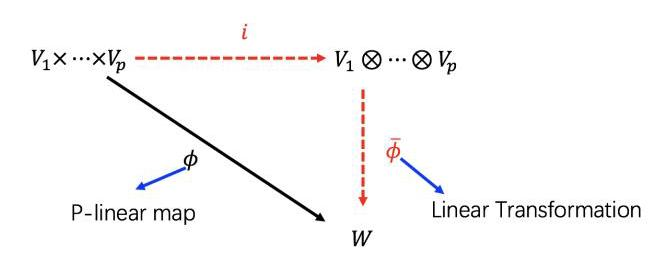
\includegraphics[max width=0.5\textwidth]{images/bo_d1h964v7aajc7382l5mg_169_640_601_665_269_0.jpg}
\end{center}
\hspace*{3em} 

In other words, \(\phi  = \bar{\phi } \circ  i\).

Corollary 14.1 Let \({T}_{i} : {\bf v}_{i} \rightarrow  {\bf v}_{i}^{\prime }\) be a linear transformation, \(1 \leq  i \leq  p\). There is a unique linear transformation

\(\left( {{T}_1 \otimes  \cdots  \otimes  {T}_{p}}\right)  : \;{\bf v}_1 \otimes  \cdots  \otimes  {\bf v}_{p} \rightarrow  {\bf v}_1^{\prime } \otimes  \cdots  \otimes  {\bf v}_{p}^{\prime }\)

atisfying \(\;\left( {{T}_1 \otimes  \cdots  \otimes  {T}_{p}}\right) \left( {{\bf v}_1 \otimes  \cdots  \otimes  {\bf v}_{p}}\right)  = {T}_1\left( {\bf v}_1\right)  \otimes  \cdots  \otimes  {T}_{p}\left( {\bf v}_{p}\right)\)

Proof. Construct the mapping

\[
\phi  : \;{\bf v}_1 \times  \cdots  \times  {\bf v}_{p} \rightarrow  {\bf v}_1^{\prime } \otimes  \cdots  \otimes  {\bf v}_{p}^{\prime }
\]

\[
\text{ with }\left( {{\bf v}_1,\ldots ,{\bf v}_{p}}\right)  \mapsto  {T}_1\left( {\bf v}_1\right)  \otimes  \cdots  \otimes  {T}_{p}\left( {\bf v}_{p}\right)
\]

which is indeed \(p\) -linear.

By the universal property, we induce the unique linear transformation

\[
\bar{\phi } : {\bf v}_1 \otimes  \cdots  \otimes  {\bf v}_{p} \rightarrow  {\bf v}_1^{\prime } \otimes  \cdots  \otimes  {\bf v}_{p}^{\prime }
\]

Notation. To make life easier, from now on, we only consider \({\bf v}_1 = \cdots  = {\bf v}_{p} = V\). Then for any linear transformation \(T : V \rightarrow  W\), we have

\[
{T}^{\otimes p} : V \otimes  \cdots  \otimes  V \rightarrow  W \otimes  \cdots  \otimes  W
\]

We use the short-hand notation \({V}^{\otimes p}\) to denote \(\underset{p\text{ terms in total }}{\underbrace{V \otimes  \cdots  \otimes  V}}\)

Final Exam Ends Here.

\subsection{Exterior Product}

Definition 14.2 A \(p\) -linear map \(\phi  : V \times  \cdots  \times  V \rightarrow  W\) is called alternating if

\(\phi \left( {{\bf v}_1,\ldots ,{\bf v}_{i},\ldots ,{\bf v}_{j},\ldots ,{\bf v}_{p}}\right)  = {\mathbf{0}}_{W}\), provided that there exists some \({\bf v}_{i} = {\bf v}_{j}\) for \(i \neq  j\).

Also, we say \(\phi\) is \(p\) -alternating

\begin{itemize}
\item Example 14.1 1. The cross product mapping
\end{itemize}

\[
\phi  : \;{\mathbb{R}}^{3} \times  {\mathbb{R}}^{3} \rightarrow  {\mathbb{R}}^{3}
\]

\[
\text{ with }\left( {v,w}\right)  \mapsto  v \times  w
\]

is alternating:

\begin{itemize}
\item \(\phi\) is bilinear
\end{itemize}

\begin{itemize}
\item \(\phi \left( {\mathbf{v},\mathbf{v}}\right)  = \mathbf{v} \times  \mathbf{v} = \mathbf{0}\).
\end{itemize}

2. The determinant mapping

\[
\phi  : \underset{n\text{ terms in total }}{\underbrace{{\mathbb{F}}^n \times  \cdots  \times  {\mathbb{F}}^n}} \rightarrow  \mathbb{F}
\]

\[
\text{ with }\left( {{\bf v}_1,\ldots ,{\bf v}_n}\right)  \mapsto  \det \left( \left\lbrack  {{\bf v}_1,{\bf v}_2,\cdots ,{\bf v}_n}\right\rbrack  \right)
\]

is alternating:

\begin{itemize}
\item \(\phi\) is \(n\) -linear by MAT 2040 knowledge
\end{itemize}

\begin{itemize}
\item \(\phi\) is alternating by MAT 2040 knowledge
\end{itemize}

Theorem 14.2 - Universal Property for exterior power. Let \(\mathrm{{Obj}} \mathrel{\text{ := }} \{ \phi  : \underset{p\text{ terms }}{\underbrace{V \times  \cdots V}} \rightarrow  W \mid\)

\(\phi\) is \(p\) -alternating map \(\}\). Then there exists \(\{ \Lambda  : V \times  \cdots  \times  V \rightarrow  E\}  \in\) Obj satisfying the following:

\begin{itemize}
\item For all \(\phi  : V \times  \cdots  \times  V \rightarrow  W \in  \mathrm{{Obj}}\), there exists unique linear transformation \(\bar{\phi } : E \rightarrow  W\) satisfying
\end{itemize}

\begin{center}
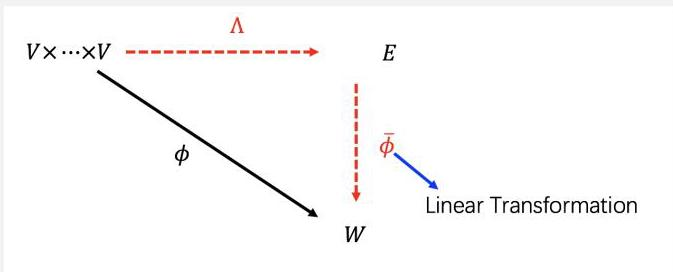
\includegraphics[max width=0.5\textwidth]{images/bo_d1h964v7aajc7382l5mg_171_635_916_673_272_0.jpg}
\end{center}
\hspace*{3em} 

In other words, \(\phi  = \bar{\phi } \circ  \Lambda\).

\section{Week 15}
\subsection{More on Exterior Product}

Reviewing. Let \(\mathrm{{Obj}} \mathrel{\text{ := }} \{ \phi  : V \times  \cdots  \times  V \rightarrow  W \mid  \phi\) is alternating \(\}\), then there exists

\[
\{ \Lambda  : V \times  \cdots  \times  V \rightarrow  E\}  \in  \mathrm{{Obj}}
\]

such that

\(\phi  = \bar{\phi } \circ  \Lambda\), where \(\bar{\phi } : E \rightarrow  W\) is the unique linear transformation

Here we give one way for constructing \(E\) :

\[
E = {V}^{\otimes p}/U,
\]

where \(U\) is spanned by vectors of the form

\[
{\bf v}_1 \otimes  \cdots  \otimes  {\bf v}_{p} \in  {V}^{\otimes p},\;{\bf v}_{i} = {\bf v}_{j}\text{ where for some }i \neq  j.
\]

For instance, \(v \otimes  v \otimes  \cdots  \otimes  {\bf v}_{p} \in  U\).

Definition 15.1 [Wedge Product] Define the wedge product space

\[
{ \land  }^{p}V \mathrel{\text{ := }} {V}^{\otimes p}/U = E,
\]

with the wedge product among vectors

\[
{\bf v}_1 \land  \cdots  \land  {\bf v}_{p} = {\bf v}_1 \otimes  \cdots  \otimes  {\bf v}_{p} + U \in  { \land  }^{p}V
\]

As a result, the mapping

\[
\land   : V \times  \cdots  \times  V \rightarrow  E \mathrel{\text{ := }} { \land  }^{p}V
\]

\[
\left( {{\bf v}_1,\ldots ,{\bf v}_{p}}\right)  \mapsto  {\bf v}_1 \land  \cdots  \land  {\bf v}_{p}
\]

will satisfy the universal property of exterior power.

Proposition 15.1 1. We have the \(p\) -linearity for \({ \land  }^{p}V\), i.e.,

\[
{\bf v}_1 \land  \cdots  \land  \left( {a{\bf v}_{i} + b{\bf v}_{i}^{\prime }}\right)  \land  \cdots  \land  {\bf v}_{p} = a\left( {{\bf v}_1 \land  \cdots  \land  {\bf v}_{i} \land  \cdots  \land  {\bf v}_{p}}\right)  + b\left( {{\bf v}_1 \land  \cdots  \land  {\bf v}_{i}^{\prime } \land  \cdots  \land  {\bf v}_{p}}\right)
\]

for \(i = 1,\ldots ,p\).

2. The wedge product is alternating:

\[
{\bf v}_1 \land  \cdots  \land  v \land  \cdots  \land  v \land  \cdots  \land  {\bf v}_{p} \mathrel{\text{ := }} {\bf v}_1 \otimes  \cdots  \otimes  v \otimes  \cdots  \otimes  v \otimes  \cdots  \otimes  {\bf v}_{p} + U
\]

\[
= 0 + U
\]

\[
= {0}_{\land {PV}}
\]

3. The wedge product reverses sign reversal property:

\[
{\bf v}_1 \land  \cdots  \land  v \land  \cdots  \land  w \land  \cdots  \land  {\bf v}_{p} =  - {\bf v}_1 \land  \cdots  \land  w \land  \cdots  \land  v \land  \cdots  \land  {\bf v}_{p}
\]

Reason: \(\left( {v + w}\right)  \land  \left( {v + w}\right)  = 0\), which implies \(v \land  w + w \land  v = 0\).

Proposition 15.2 1. If \(\dim \left( V\right)  = n\), and \(0 \leq  p \leq  n\), then

\[
\dim \left( {{ \land  }^{p}V}\right)  = \left( \begin{array}{l} n \\  p \end{array}\right)
\]

2. For all linear operators \(T : V \rightarrow  V\), there is an unique linear operator from \({ \land  }^{p}V\) to \(\land  {PV} :\)

\[
{T}^{{ \land  }^{p}} : \;{ \land  }^{p}V \rightarrow  { \land  }^{p}V
\]

\[
\text{ with }{\bf v}_1 \land  \cdots  \land  {\bf v}_{p} \mapsto  T\left( {\bf v}_1\right)  \land  \cdots  \land  T\left( {\bf v}_{p}\right)
\]

Proof. 1. Let \(\left\{  {{\bf v}_1,\ldots ,{\bf v}_n}\right\}\) be basis of \(V\), then \(\left\{  {{\bf v}_{{i}_1} \otimes  \cdots  \otimes  {\bf v}_{{i}_{p}} \mid  1 \leq  {i}_{k} \leq  n}\right\}\) forms basis of \({V}^{\otimes p}\). Note that \(\left\{  {{\bf v}_{{i}_1} \land  \cdots  \land  {\bf v}_{{i}_{p}} \mid  1 \leq  {i}_{k} \leq  n}\right\}\) spans \({ \land  }^{p}V\), since \({\pi }_{V} : V \rightarrow  V/U\) is surjective. We claim that

\[
\mathcal{B} = \left\{  {{\bf v}_{{i}_1} \land  \cdots  \land  {\bf v}_{{i}_{p}} \mid  1 \leq  {i}_1 < {i}_2 < \cdots  < {i}_{p} \leq  n}\right\}
\]

is a basis of \({ \land  }^{p}V\)

\begin{itemize}
\item \(\mathcal{B}\) spans \({ \land  }^{p}V\) : we can use (3) in proposition (15.1) to "rearrange" the indices \({j}_1,\ldots ,{j}_{p}\) into ascending order, and \(\operatorname{span}\left( \mathcal{B}\right)  = \operatorname{span}\left\{  {{\bf v}_{{i}_1} \land  \cdots  \land  {\bf v}_{{i}_{p}} \mid  1 \leq  {i}_{k} \leq  n}\right\}\).
\end{itemize}

\begin{itemize}
\item We omit the proof that \(\mathcal{B}\) is linear independent due to time limit.
\end{itemize}

The numbre of vectors in \(\mathcal{B}\) is equal to \(\left( \begin{array}{l} n \\  p \end{array}\right)\).

\subsection{The Determinant}

Previous Approach for defining determinant. We define the determinant for \(A = {M}_{n \times  n}\left( \mathbb{F}\right)\) directly. From such complicated definition, we come up with \(\det \left( \mathbf{{AB}}\right)  =\)  \(\det \left( A\right) \det \left( B\right)\), which implies that the similar matrices share with the same determinant, then we define the determinant for any linear operator \(T : V \rightarrow  V\) as

\[
\det \left( T\right)  = \det \left( {\left( T\right) }_{\mathcal{B},\mathcal{B}}\right) ,\;\text{ for some basis }\mathcal{B}\text{ of }T
\]

New Approach. We will define \(\det \left( T\right)\) for linear operators without fixing a basis, and then we will imply \(\det \left( {T \circ  S}\right)  = \det \left( T\right) \det \left( S\right)\) easily. Then \(\det \left( A\right)\) for \(A \in  {M}_{n \times  n}\left( \mathbb{F}\right)\) belongs to our special case.

Definition 15.2 [Determinant for Linear Operators]

1. Suppose that \(\dim \left( V\right)  = n\), then

\[
\dim \left( {{ \land  }^nV}\right)  = \left( \begin{array}{l} n \\  n \end{array}\right)  = 1
\]

More precisely, for any basis \(\left\{  {{\bf v}_1,\ldots ,{\bf v}_n}\right\}\) of \(V\), we have \({ \land  }^n\left( V\right)  = \operatorname{span}\left\{  {{\bf v}_1 \land  \cdots  \land  {\bf v}_n}\right\}\). 2. Note tht \({T}^{{ \land  }^n} : { \land  }^nV \rightarrow  { \land  }^nV\) is a linear operator on \({ \land  }^nV \cong  \mathbb{F}\). Therefore, for all \(\tau  \in  { \land  }^nV\), there exists \(\alpha_{T} \in  \mathbb{F}\) such that

\[
{T}^{{ \land  }^n}\left( \tau \right)  = \alpha_{T}\tau
\]

3. Now we define

\[
\det \left( T\right)  = \alpha_{T}
\]

This definition of determinant does not depend on any choice of basis of \(V\).

1. Suppose that \(T = I : V \rightarrow  V\) be identity. Take a basis \(\left\{  {{\bf v}_1,\ldots ,{\bf v}_n}\right\}\)

of \(V\), then

\[
{T}^{{ \land  }^n}\left( {{\bf v}_1 \land  \cdots  \land  {\bf v}_n}\right)  = T\left( {\bf v}_1\right)  \land  \cdots  \land  T\left( {\bf v}_n\right)
\]

Or equivalently,

\[
\det \left( T\right)  \cdot  \left( {{\bf v}_1 \land  \cdots  \land  {\bf v}_n}\right)  = {\bf v}_1 \land  \cdots  \land  {\bf v}_n
\]

Therefore, \(\det \left( T\right)  = 1\).

2. Suppose that \(T : V \rightarrow  V\) is diagonalizable with \(\left\{  {{\bf w}_1,\ldots ,{\bf w}_n}\right\}\) forming eigen-basis of \(T\).

As a result,

\[
{T}^{{ \land  }^n}\left( {{\bf w}_1 \land  \cdots  \land  {\bf w}_n}\right)  = T\left( {\bf w}_1\right)  \land  T\left( {\bf w}_2\right) \cdots  \land  T\left( {\bf w}_n\right) ,
\]

which implies

\[
\det \left( T\right) \left( {{\bf w}_1 \land  \cdots  \land  {\bf w}_n}\right)  = \left( {{\lambda }_1{\bf w}_1}\right)  \land  \cdots  \land  \left( {{\lambda }_n{\bf w}_n}\right) ,
\]

which implies

\[
\det \left( T\right) {\bf w}_1 \land  \cdots  \land  {\bf w}_n = \left( {{\lambda }_1\cdots {\lambda }_n}\right) {\bf w}_1 \land  \cdots  \land  {\bf w}_n,
\]

i.e., \(\det \left( T\right)  = {\lambda }_1\cdots {\lambda }_n\).

Proposition 15.3 Let \(T,S : V \rightarrow  V\) be linear transformations, then

\[
{\left( T \circ  S\right) }^{{ \land  }^{p}} : \;{ \land  }^{p}V \rightarrow  { \land  }^{p}V
\]

\[
\text{ with }{T}^{{ \land  }^{p}},{S}^{{ \land  }^{p}} : { \land  }^{p}V \rightarrow  { \land  }^{p}V
\]

satisfies

\[
{\left( T \circ  S\right) }^{{ \land  }^{p}} = \left( {T}^{{ \land  }^{p}}\right)  \circ  \left( {S}^{{ \land  }^{p}}\right)
\]

Proof. Pick any basis \(\left\{  {{\bf v}_{{i}_1} \land  \cdots  \land  {\bf v}_{{i}_{p}} \mid  1 \leq  {i}_1 < \cdots  < {i}_{p} \leq  n}\right\}\) of \({ \land  }^{p}V\). Then

\[
{\left( T \circ  S\right) }^{{ \land  }^{p}}\left( {{\bf v}_{{i}_1} \land  \cdots  \land  {\bf v}_{{i}_{p}}}\right)  = \left( {T \circ  S}\right) \left( {\bf v}_{{i}_1}\right)  \land  \cdots  \land  \left( {T \circ  S}\right) \left( {\bf v}_{{i}_{p}}\right)
\]

On the other hand,

\[
\left( {T}^{{ \land  }^{p}}\right)  \circ  \left( {S}^{{ \land  }^{p}}\right) \left( {{\bf v}_{{i}_1} \land  \cdots  \land  {\bf v}_{{i}_{p}}}\right)  = \left( {T}^{{ \land  }^{p}}\right) \left( {S\left( {\bf v}_{{i}_1}\right)  \land  \cdots  \land  S\left( {\bf v}_{{i}_{p}}\right) }\right)
\]

\[
= \left( {T \circ  S}\right) \left( {\bf v}_{{i}_1}\right)  \land  \cdots \left( {T \circ  S}\right) \left( {\bf v}_{{i}_{p}}\right)
\]

\begin{corollary}
\[
\det \left( {T \circ  S}\right)  = \det \left( T\right) \det \left( S\right)
\]
\end{corollary}

Proof. Pick any basis \(\left\{  {{\bf v}_1 \land  \cdots  \land  {\bf v}_n}\right\}\) of \({ \land  }^nv\), then

\[
\det \left( {T \circ  S}\right) {\bf v}_1 \land  \cdots  \land  {\bf v}_n = {\left( T \circ  S\right) }^{{ \land  }^n}{\bf v}_1 \land  \cdots  \land  {\bf v}_n
\]

\[
= \left( {T}^{{ \land  }^n}\right)  \circ  \left( {\left( {S}^{{ \land  }^n}\right) {\bf v}_1 \land  \cdots  \land  {\bf v}_n}\right)
\]

\[
= \left( {T}^{{ \land  }^n}\right) \left( {\det \left( S\right) {\bf v}_1 \land  \cdots  \land  {\bf v}_n}\right)
\]

\[
= \det \left( S\right) {T}^{{ \land  }^n}\left( {{\bf v}_1 \land  \cdots  \land  {\bf v}_n}\right)
\]

\[
= \det \left( S\right) \det \left( T\right) {\bf v}_1 \land  \cdots  \land  {\bf v}_n
\]

Therefore, \(\det \left( {T \circ  S}\right)  = \det \left( T\right) \det \left( S\right)\).

Theorem 15.1 Let \(V = {\mathbb{F}}^n\), and

\(T : \;V \rightarrow  V\)

with \(T\left( \mathbf{v}\right)  = \mathbf{{Av}},\;A \in  {M}_{n \times  n}\left( \mathbb{F}\right)\)

Then \(\det \left( T\right)  = \det \left( A\right)\)

Proof. Take \(\left\{  {{e}_1,\ldots ,{e}_n}\right\}\) as the usual basis of \(V \equiv  {\mathbb{F}}^n\), then

\[
\det \left( T\right) {e}_1 \land  \cdots  \land  {e}_n = T\left( {e}_1\right)  \land  \cdots T\left( {e}_n\right)
\]

\[
= {a}_1 \land  \cdots  \land  {a}_n
\]

where \({a}_{i}\) denotes the \(i\) -th column of \(A\).

As we have studied before [c.f. p141 in MAT 2040 Notebook], the previous definition of determinant is based on three basic properties. It suffices to show these three basis properties:

1. The determinant of the \(n\) by \(n\) identity matrix is 1 : See part (1) in Example (15.1)

2. The determianant changes sign when two columns (w.l.o.g., "rows" are relaced with "columns") are exchanged: due to the sign reversal property for wedge product

3. The determinant is a linear function of each column separately, i.e.,

\[
{a}_1 \land  \cdots  \land  \left( {t{a}_{i}}\right)  \land  \cdots  \land  {a}_n = t\left( {{a}_1 \land  \cdots  \land  {a}_{i} \land  \cdots  \land  {a}_n}\right)
\]

Once we verify these three properties, we conclude that the explicit formula for \(\det \left( A\right)\) is a special case for our new definition.

Or we can come into the previous definition for determinant directly. For instance, consider the mapping

\[
T : \;{\mathbb{R}}^2 \rightarrow  {\mathbb{R}}^2
\]

\[
\text{ with }T\left( \begin{array}{l} x \\  y \end{array}\right)  = \left( \begin{array}{ll} a & b \\  c & d \end{array}\right) \left( \begin{array}{l} x \\  y \end{array}\right)
\]

Then we imply

\[
\det \left( T\right) \left( {{e}_1 \land  {e}_2}\right)  = \left( \begin{array}{l} a \\  c \end{array}\right)  \land  \left( \begin{array}{l} b \\  d \end{array}\right)
\]

\[
= \left( {a{e}_1}\right)  \land  \left( {b{e}_1}\right)  + \left( {a{e}_1}\right)  \land  \left( {d{e}_2}\right)  + \left( {c{e}_2}\right)  \land  \left( {d{e}_1}\right)  + \left( {c{e}_2}\right)  \land  \left( {d{e}_2}\right)
\]

\[
= \left( {ad}\right) {e}_1 \land  {e}_2 + \left( {bc}\right) {e}_2 \land  {e}_1
\]

\[
= \left( {{ad} - {bc}}\right) {e}_1 \land  {e}_2
\]

Therefore, we imply \(\det \left( T\right)  = {ad} - {bc}\).
\end{document}